\documentclass[12pt,letterpaper]{book}
%%%%%%%%%%%%%%%%%%%%%%%%%%%%%%
%Force pdflatex processing even with "$ latex" (required by arXiv)
\pdfoutput=1
%%%%%%%%%%%%%%%%%%%%%%%%%%%%%
\usepackage[utf8]{inputenc}
\usepackage{amsmath}
\usepackage{amssymb}
\usepackage{amsthm}
\usepackage[colorlinks=true]{hyperref}
\usepackage{graphicx}
\usepackage{cancel}
\usepackage[svgnames]{xcolor}
\usepackage[english]{babel}
\usepackage{bm}
\usepackage{simplewick}
\usepackage[toc,page]{appendix}
\graphicspath{{figures/}}
\usepackage{listings}
\usepackage[displaymath,textmath,sections,graphics,floats]{preview}
%%%%%%%%%
\newcommand{\timesm}{\times}
\newcommand{\pmm}{\pm}
\newcommand{\mpm}{\mp}
\usepackage{comment}
\includecomment{inprogress}
\specialcomment{inprogress}
{\begingroup\itshape \textbf{Begin Draft:}}{\textbf{End Draft.} \medskip \endgroup}
\excludecomment{inprogress}

\includecomment{borrar}
\specialcomment{borrar}
{\begingroup\itshape \textbf{Begin Draft:}}{\textbf{End Draft.} \medskip \endgroup}
\excludecomment{borrar}

\includecomment{details}
\specialcomment{details}
{\begingroup}{\endgroup}
%\excludecomment{details}
\PreviewEnvironment{details}
%%%%%%%%%%%%%%%%%%%%%%%%%%%%%%
%%Beamer compability layer
%to compile beamer use beyond.beamer.tex
\includecomment{frame}
\specialcomment{frame}
{\begingroup}{\endgroup}
%\excludecomment{frame}
%%%%%%%%%%%%%%%%%%%%%%%%%%%%%


%\usepackage{bbold}
\setlength{\textwidth}{180mm}
\setlength{\oddsidemargin}{-1cm}
\setlength{\evensidemargin}{-1cm}
%\setlength{\topmargin}{-40pt}
\def\lt{<} % compatibility with instiki
\def\gt{>} % compatibility with instiki
\newtheoremstyle{example}{\topsep}{\topsep}%
     {}%         Body font
     {}%         Indent amount (empty = no indent, \parindent = para indent)
     {\bfseries}% Thm head font
     {}%        Punctuation after thm head
     {\newline}%     Space after thm head (\newline = linebreak)
     {\thmname{#1}\thmnumber{ #2}\thmnote{ #3}}%         Thm head spec

   \theoremstyle{example}
   \newtheorem{example}{Example}[subsection]
%%comment the aproppiate line
\newcommand{\tofc}[1]{#1} % if full
%\renewcommand{\tofc}[1]{} %if  \includeonly{chapter1}
%\includeonly{feynman}

 \lstset{language=python
%,inputencoding=utf8
%,showspaces=false
%{\small Hola} {\footnotesize Hola} {\scriptsize Hola} {\tiny Hola}
,basicstyle=\small\ttfamily
%,basicstyle=\small\sffamily,
,keywordstyle=\color{blue}
,commentstyle=\normalfont\ttfamily\color{red}
,stringstyle=\color{Green}
%,numbers=left
%,numberstyle=\tiny
,frame=b
,inputencoding=utf8
,extendedchars=true
,columns=fullflexible
,showstringspaces=false
%,backgroundcolor=\color{lightgray}
,texcl=true
}
%%%%%%%%%%%%%%%%%%%
%\includeonly{sndquantization}
\includeonly{renormalization}
\begin{document}
\renewcommand{\thepage}{\roman{page}}
\begin{titlepage}
  \begin{center}

    
\textbf{\huge    Detailed lecture notes in Quantum Field Theory}

    

\vspace{4cm}
 Diego Restrepo\\
Instituto de Física\\
Universidad de Antioquia\\
2012
    
  \end{center}
\end{titlepage}



\chapter*{License}


\noindent

\includegraphics[scale=0.5]{cc} All materials are licensed under the \href{http://creativecommons.org/licenses/by-sa/3.0/us/}{Creative Commons Attribution-Share Alike 3.0 United States License.}
%%% Local Variables: 
%%% mode: latex
%%% TeX-master: "beyond"
%%% End: 




\tofc{
\renewcommand{\thepage}{\roman{page}}
\tableofcontents{}

\newpage{}
}

\renewcommand{\thepage}{\arabic{page}}
\setcounter{page}{1}



%$x^2$
%instiki:category: QuantumFieldTheory
%instiki:
%instiki:***
%instiki:
%instiki:[[Beyond|Contents]]
%instiki:
%instiki:***

\chapter*{Introduction}
\label{cha:introduction} %noinstiki

\addcontentsline{toc}{chapter}{Introduction} %noinstiki

We have organized the topics in order of complexity, and, in the same
spirit than in  previous book \cite{lsm}, we have tried to write the
calculations as detailed as possible. In
Chapter 
\ref{cha:second-quantization} %noinstiki [[Chapter II]]
we included the building blocks
of quantum field theory, in Chapter 
\ref{cha:s-matrix} %noinstiki [[Chapter III]]
we introduce
the $S$--matrix in the Scr\"odinger Picture separating the kinematical
and normalization factors from the matrix element. Then the expressions
for the decay rates and cross sections are obtained. The explicit
calculation of the matrix element from the expansion of the
$S$--matrix to obtain the Feynman rules, is postponed to Chapter
\ref{chap:fr}. %noinstiki [[Chapter V]].
In Chapter 
\ref{cha:two-body-decays} %noinstiki [[Chapter IV]]
we use the Feynman
rules necessary to calculates the matrix element, and develop the
techniques associated to the squaring of the matrix element. In
Chapter 
\ref{chap:fr} %noinstiki [[Chapter V]]
we obtain the Feynman rules used in two body
decays directly from the first order expansion of the $S$--matrix in
the interaction picture. The subsequent chapters have applications of
the techniques developed to the calculation of tree-level, 
Chapter 
\ref{cha:three-body-decays} %noinstiki [[Chapter V]]
and loop processes.


This notes are based in books \cite{Maggiore:2005qv}, \cite{Mandl:1985bg}, \cite{Lahiri:2005sm}.  In each Chapter or Section the main reference used is cited. Also, we have included material developed by students Juan Alberto Yepez, Jos\'e David Ruiz \'Alvarez. This notes are written in English, because at this level it is expected that any physics student be fluently in reading technical texts in this language.

Some parts are still in Spanish. 

This work have been partially supported by ``Dedicaci\'on Exclusiva 2008-2009''  project: RR 26663

%%% Local Variables: 
%%% mode: latex
%%% TeX-master: "beyond"
%%% End:

\chapter{Classical Field Theory}
\label{chap:cft}

This chapter is a summary of the main topics developed in the course ``Hacia la teoría cuántica de campos'' \cite{lsm}. We will introduce special relativity as the necessary ingredient to guarantee the local conservation of electric charge in quantum mechanics. The symmetries of the electromagnetic Lagrangian will be extended to include the electron, as one Dirac spinor. The resulting Quantum Electrodynamics theory will be used as a paradigm to explain the other fundamental interactions.

\section{Lagrangian Formulation}
\label{sec:lagr-form}
\subsection{Ecuaciones de Euler-Lagrange}

Definamos
\begin{equation}
  \label{eq:dmu}
  \partial_\mu=\frac{\partial}{\partial x^\mu},
  \end{equation}
%%aclarar que un indice en el denomindador bla bla bla
En tres dimensiones, la acción de la se puede escribir como:
\begin{equation}
  \label{eq:Scall3d}
  S[\phi,\partial_\mu\phi]=\int_{R}d^4x\mathcal{L}(\phi,\partial_\mu\phi)
\end{equation}
donde $d^4x=d t\,d x\, d y\,d z$.  Considere primero una variación sólo de
los campos, tal que ($x=x^\mu)$
\begin{equation}
  \label{eq:deltaphi}
  \delta\phi(x)=\phi'(x)-\phi(x)
\end{equation}
De otro lado, con $\delta x=x'-x$, la expansión de Taylor para $f(x+\delta x)$ es
\begin{equation}
  f(x+\delta x)=f(x)+\frac{\partial f}{\partial x}\delta x+\cdots 
\end{equation}
Para $\mathcal{L}$, tenemos de la ec.~\eqref{eq:deltaphi}
\begin{align}
  \mathcal{L}(\phi',\partial_\mu\phi')&=\mathcal{L}(\phi+\delta\phi,\partial_\mu\phi+\partial_\mu(\delta\phi))\nonumber\\
  &=\mathcal{L}+\frac{\partial\mathcal{L}}{\partial\phi}\delta\phi+\frac{\partial\mathcal{L}}{\partial(\partial_\mu\phi)}\partial_\mu(\delta\phi)
\end{align}
Entonces, de imponer que $\delta S=0$, tenemos
\begin{align}
  \delta S&=S'-S=\int_{R}d^4x\,\mathcal{L}(\phi',\partial_\mu\phi')-\int_{R}d^4x\,\mathcal{L}(\phi,\partial_\mu\phi)\nonumber\\
&=\int_{R}d^4x\,
\left[
\frac{\partial\mathcal{L}}{\partial\phi}\delta\phi+\frac{\partial\mathcal{L}}{\partial(\partial_\mu\phi)}\partial_\mu(\delta\phi)
\right]\nonumber\\
 &=\int_{R}d^4x\,
  \left\{ 
    \frac{\partial\mathcal{L}}{\partial\phi}-\left[\partial_\mu\left(
      \frac{\partial\mathcal{L}}{\partial(\partial_\mu\phi)}
    \right)\right]
  \right\}\delta\phi+\int_{R}d^4x\,
    \partial_\mu\left[
      \frac{\partial\mathcal{L}}{\partial(\partial_\mu\phi)}\delta\phi
    \right]\nonumber\\
\label{eq:1qft}
\delta S&=\int_{R}d^4x\,
  \left\{ 
    \frac{\partial\mathcal{L}}{\partial\phi}-    
    \left[\partial_\mu\left(
      \frac{\partial\mathcal{L}}{\partial(\partial_\mu\phi)}
    \right)\right]
  \right\}\delta\phi+\int_{\sigma}\left[
      \frac{\partial\mathcal{L}}{\partial(\partial_\mu\phi)}\delta\phi
    \right]\,d\sigma_\mu=0.
\end{align}
Donde hemos aplicado el Teorema de Gauss
\begin{equation}
\int_V\boldsymbol{\nabla}\cdot\mathbf{A}\,d^3x=
 \int_S\mathbf{A}\cdot d\mathbf{S}\,
\end{equation}
generalizado a cuatro dimensiones. Como la variación de $\delta\phi$ es cero sobre la hipersuperficie $\sigma$ resulta 
\begin{equation}
  \int_{R}d^4x\,
  \left\{ 
    \frac{\partial\mathcal{L}}{\partial\phi}-
   \left[\partial_\mu\left(
      \frac{\partial\mathcal{L}}{\partial(\partial_\mu\phi)}
    \right)\right]
  \right\}\delta\phi=0.
\end{equation}
Como $\delta\phi$ es cualquier posible variación entre las fronteras de la hipersuperficie, el integrando debe anularse y resultan las ecuaciones de Euler-Lagrange:
\begin{equation}
\label{eq:eelcallfmu}
 \partial_\mu
  \left[
    \frac{\partial\mathcal{L}}{\partial
      (\partial_\mu\phi)}
  \right]-\frac{\partial\mathcal{L}}{\partial\phi}=0.
\end{equation}
La densidad Lagrangiana
\begin{align}
  \mathcal{L}'=\mathcal{L}+\partial_\mu(\eta(x))
\end{align}
donde $\eta(x)$ es cualquier función de los campos de la densidad Lagrangiana original, da lugar a la Acción
\begin{align}
  S'=\int_{R}d^4x\,\mathcal{L}'=&\int_{R}d^4x\,\mathcal{L}+\int_R d^4x\,\partial_\mu\eta\nonumber\\
  =&\int_{R}d^4x\,\mathcal{L}+\int_\sigma \eta d\sigma_\mu\nonumber\\
  =&S\,,
\end{align}
para una hipersuperficie suficientemente grande. De modo que dos densidades lagrangianas que difieran solo en derivadas totales dan lugar a la misma Acción.

Usando el principio de mínima acción en términos del campo $\phi$, tenemos que para la densidad Lagrangiana~\eqref{eq:call2}
\begin{align}
  \mathcal{L}=&\frac{1}{2}  \left[
  \frac{1}{v^2}\left(\frac{\partial\phi}{\partial t}\right)^2-\left(\frac{\partial\phi}{\partial z}\right)^2
\right],
\end{align}
las ecuaciones de Euler-Lagrange~\eqref{eq:eelcallfmu}
\begin{align}
  \partial_0\left[\frac{\partial\mathcal{L}}{\partial(\partial_0\phi)}\right]+
\partial_3\left[\frac{\partial\mathcal{L}}{\partial(\partial_3\phi)}\right]
-\frac{\partial\mathcal{L}}{\partial\phi}=&0\nonumber\\
  \frac{\partial}{\partial t}\left[\frac{\partial\mathcal{L}}{\partial(\partial\phi/\partial t)}\right]+
\frac{\partial}{\partial z}\left[\frac{\partial\mathcal{L}}{\partial(\partial\phi/\partial z)}\right]
=&0\nonumber\\
 \frac{1}{v^2}\frac{\partial}{\partial t}\left[\frac{\partial\phi}{\partial t}\right]
-\frac{\partial}{\partial z}\left[\frac{\partial\phi}{\partial z}\right]=&0\nonumber\\
 \frac{1}{v^2}\frac{\partial^2\phi}{\partial t^2}-\frac{\partial^2\phi}{\partial z^2}=&0\,,
\end{align}
que corresponde a la ecuación de onda.

Generalizando a tres dimensiones vemos que la ecuación para una onda propagandose a una velocidad $v$,
\begin{equation}
     \frac{1}{v^2}\frac{\partial^2\phi}{\partial t^2}-\nabla^2\phi=0\,,
\end{equation}
proviene de una densidad Lagrangiana (hasta derivadas totales)
\begin{align}
    \mathcal{L}=&\frac{1}{2}\left[
\frac{1}{v^2}\left(\frac{\partial\phi}{\partial t}
  \right)^2-\boldsymbol{\nabla}\phi\cdot\boldsymbol{\nabla}\phi \right]\nonumber\\
    =&\frac{1}{2}\left[
      \frac{1}{v^2}{\partial_0\phi}\,{\partial_0\phi}-{\partial_i\phi}\,{\partial_i\phi}
   \right]\,.
\end{align}
\subsection{Teorema de Noether para simetrías internas}
Para un campo complejo la ec.~(\ref{eq:Scall3d}) se generaliza a
\begin{equation}
  S[\phi,\phi^*,\partial_\mu\phi,\partial_\mu\phi^*]=\int_{R}d^4x\,\mathcal{L}(\phi,\phi^*,\partial_\mu\phi,\partial_\mu\phi^*)
\end{equation}
Usando el mismo procedimiento, se obtiene
\begin{align}
  \label{eq:130qft}
   \delta S=&\int_{R}d^4x\,
  \left\{ 
    \frac{\partial\mathcal{L}}{\partial\phi}-
  \left[\partial_\mu\left(
      \frac{\partial\mathcal{L}}{\partial(\partial_\mu\phi)}
    \right)\right]
  \right\}\delta\phi
+\int_{R}d^4x\,
  \left\{ 
    \frac{\partial\mathcal{L}}{\partial\phi^*}-
  \left[\partial_\mu\left(
      \frac{\partial\mathcal{L}}{\partial(\partial_\mu\phi^*)}
    \right)\right]
  \right\}\delta\phi^*\nonumber\\
&+\int_{R}d^4x\,
    \partial_\mu\left[
      \frac{\partial\mathcal{L}}{\partial(\partial_\mu\phi)}\delta\phi+
      \delta\phi^*\frac{\partial\mathcal{L}}{\partial(\partial_\mu\phi^*)}
    \right]=0.
\end{align}
Usando de nuevo el Teorema de Gauss resultan las ecuaciones de Euler Lagrange para $\phi$ y $\phi^*$
\begin{equation}
\label{eq:132qft}
  \partial_\mu
  \left[
    \frac{\partial\mathcal{L}}{\partial
      (\partial_\mu\phi)}
  \right]-\frac{\partial\mathcal{L}}{\partial\phi}=0, \qquad
  \partial_\mu
  \left[
    \frac{\partial\mathcal{L}}{\partial
      (\partial_\mu\phi^*)}
  \right]-\frac{\partial\mathcal{L}}{\partial\phi^*}=0.
\end{equation}
De otro lado, si asumimos que $\phi$ y $\phi^*$ satisfacen las ecuaciones de Euler--Lagrange, en lugar de asumir que $\delta\phi$ y $\delta\phi^*$ se anulan sobre la hipersuperficie, los dos primeros términos de la ec.~(\ref{eq:130qft}) se anulan y tendremos que para que $\delta S=0$:
\begin{equation}
  \label{eq:jmu}
  \int_{R}d^4x\,(\partial_\mu J^\mu)=0,
\end{equation}
donde,
\begin{equation}
  \label{eq:jmuphi}
 J^\mu= \left[
      \frac{\partial\mathcal{L}}{\partial(\partial_\mu\phi)}
    \right]\delta\phi+\delta\phi^*\left[
      \frac{\partial\mathcal{L}}{\partial(\partial_\mu\phi^*)}
    \right]
\end{equation}
Entonces $J^\mu$ satisface la ecuación de continuidad:
\begin{align}
  \label{eq:conti}
  \partial_\mu J^\mu&=0\\
\frac{\partial J^0}{\partial t}+\boldsymbol{\nabla}\cdot\mathbf{J}&=0
\end{align}
Integrando con respecto al volumen
\begin{align}
  &\int_V\frac{\partial J^0}{\partial t}\,d^3x+\int_V\boldsymbol{\nabla}\cdot\mathbf{J}\,d^3x=0,\nonumber\\
  &\int_V\frac{\partial J^0}{\partial t}\,d^3x+\int_S\mathbf{J}\cdot d\mathbf{S}=0,
\end{align}
Escogiendo una superficie suficientemente grande que abarque toda la fuente de densidad $\rho=J^0$, de la corriente $\mathbf{J}$, el segundo integrando es cero y
\begin{equation}
  \frac{d}{dt}\int_V\rho\,d^3x=0.
\end{equation}
Este resultado es conocido como Teorema de Noether. Éste establece que para
toda transformación continua del tipo \eqref{eq:deltaphi}, debe
existir una cantidad conservada, $dQ/dt=0$, que en este caso corresponde a
\begin{equation}
  \label{eq:qcons}
  Q=\int_V \rho\,d^3x.
\end{equation}


\subsection{Teorema de Noether para simetrías externas}
\label{sec:teorema-de-noether}
Para el caso de una simetría externas, por ejemplo la correspondiente a una traslación espacio--temporal
\begin{align}
  x^\mu\to{x'}^\mu=&x^\mu+\delta a^\mu\nonumber\\
  \delta x^\mu=&\delta a^\mu
\end{align}

tenemos
\begin{align}
  \phi'(x')&=\phi'(x+\delta a)\\
  &\approx\phi'(x)+\frac{\partial\phi'(x)}{\partial x^\mu}\delta a^\mu\\
  &=[\phi(x)+\delta\phi(x)]+\frac{\partial}{\partial x^\mu}[\phi(x)+\delta\phi(x)]\delta a^\mu\\
  &\approx\phi(x)+\delta\phi(x)+\frac{\partial\phi(x)}{\partial x^\mu}\delta a^\mu,
\end{align}
donde, por simplicidad, $\phi$ es de nuevo un campo real, y en el último paso hemos despreciado un término de orden $\delta\phi\delta a^\mu$. Entonces,
\begin{equation}
  \label{eq:Deltaf}
  \Delta\phi(x)\equiv\phi'(x')-\phi(x)=\delta\phi(x)+\frac{\partial\phi(x)}{\partial x^\mu}\delta a^\mu.
\end{equation}
Para una traslación, $\Delta\phi(x)=0$, ver figura 
\ref{fig:trasla}. %noinstiki([trasla](#fig:trasla)).
De modo que
\begin{equation}
  \label{eq:dmuxmu}
  \delta\phi=-(\partial_\mu\phi)\delta a^\mu,
\end{equation}
y la transformación del campo $\phi$ como consecuencia de la traslación es
\begin{align}
  \phi(x)\to\phi'(x)=\phi(x)+\delta\phi(x)=\phi(x)-(\partial_\mu\phi(x))\delta a^\mu\,.
\end{align}
%noinstiki

\begin{figure} %noinstiki
  \centering %noinstiki
  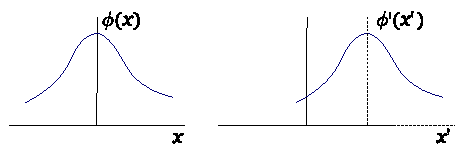
\includegraphics{trasla} %noinstiki
  \caption{Traslación de función y coordenadas en una dimensión: $\phi(x)=\phi'(x')$ } %noinstiki
  \label{fig:trasla} %noinstiki
\end{figure} %noinstiki<div id="fig:trasla">Figura trasla:Traslación de función y coordenadas $\phi(x)=\phi(x')$ </div>
%noinstiki![trasla](http://gfif.udea.edu.co/figfs/trasla.png)
%noinstiki
Si $a^\mu$ es constante (un análisis más general es hecho en \cite{r})
\begin{equation}
  d^4x'=d^4x
\end{equation}
En este caso, asumiendo que el campo satisface las ecuaciones de
Euler-Lagrange y usando la ec.~\eqref{eq:dmuxmu} y (\ref{eq:eelcallfmu}) tenemos
\begin{align}
  \delta S&=\int_{R}d^4x\,\mathcal{L}(\phi',\partial_\mu\phi',{x'}^\mu)-\int_{R}d^4x\,\mathcal{L}(\phi(x),\partial_\mu\phi(x),x)\nonumber\\
  &=\int_{R}d^4x\,\mathcal{L}(\phi+\delta\phi,\partial_\mu\phi+\partial_\mu(\delta\phi),x^\mu+\delta a^\mu)-\int_{R}d^4x\,\mathcal{L}\nonumber\\
  &\approx\int_{R}d^4x\,
  \left[\mathcal{L}+
    \frac{\partial\mathcal{L}}{\partial\phi}\delta\phi+\frac{\partial\mathcal{L}}{\partial(\partial_\mu\phi)}\partial_\mu(\delta\phi)+
    (\partial_\mu\mathcal{L})\delta a^\mu\right]-\int_{R}d^4x\,\mathcal{L}\nonumber\\
  &=\int_{R}d^4x\,
  \left[
    \frac{\partial\mathcal{L}}{\partial\phi}\delta\phi+\frac{\partial\mathcal{L}}{\partial(\partial_\mu\phi)}\partial_\mu(\delta\phi)+
    (\partial_\mu\mathcal{L})\delta a^\mu\right]\nonumber\\
  &=\int_{R}d^4x\,
  \left\{ 
    \left[\partial_\mu\left(\frac{\partial\mathcal{L}}{\partial(\partial_\mu\phi)}
    \right)\right]\delta\phi+\frac{\partial\mathcal{L}}{\partial(\partial_\mu\phi)}\partial_\mu(\delta\phi)+
    (\partial_\mu\mathcal{L})\delta a^\mu\right\}\nonumber\\
  &=\int_{R}d^4x\left\{ 
    \partial_\mu\left[\frac{\partial\mathcal{L}}{\partial(\partial_\mu\phi)}\delta\phi\right]
  +(\partial_\mu\mathcal{L})\delta a^\mu\right\}\nonumber\\
   &=\int_{R}d^4x\,\partial_\mu\left\{ 
    \frac{\partial\mathcal{L}}{\partial(\partial_\mu\phi)}\delta\phi
  +\mathcal{L}\delta a^\mu\right\}\nonumber\\
   &=\int_{R}d^4x\,\partial_\mu\left\{ 
    -\frac{\partial\mathcal{L}}{\partial(\partial_\mu\phi)}\partial_\nu\phi\delta a^\nu
  +\mathcal{L}\delta a^\mu\right\}\nonumber\\
   &=\int_{R}d^4x\,\partial_\mu\left\{ 
    -\frac{\partial\mathcal{L}}{\partial(\partial_\mu\phi)}\partial_\nu\phi\delta a^\nu
  +\mathcal{L}\delta^\mu_\nu(\delta a^\nu)\right\}\nonumber\\
    &=\int_{R}d^4x\,
    \partial_\mu\left\{\left[
      -\frac{\partial\mathcal{L}}{\partial(\partial_\mu\phi)}(\partial_\nu\phi)
      +\delta^\mu_\nu\mathcal{L}
    \right]\delta a^\nu\right\}\nonumber\\
    \label{eq:2qft}
\end{align}

\begin{align}
    &=\int_{R}d^4x\,
    \partial_\mu \left(T^\mu_\nu\delta a^\nu
  \right)=0.
\end{align}
Y por consiguiente
\begin{equation}
  \partial_\mu T^\mu_\nu\delta a^\nu=0,
\end{equation}
De modo que para cada $\nu$, con $\delta a^\nu\neq0$, se satisface:

\begin{equation}
  \label{eq:131qft}
  \partial_\mu T^\mu_\nu=0,
\end{equation}
donde
\begin{equation}
  \label{eq:tmunu}
    T^\mu_\nu=\frac{\partial\mathcal{L}}{\partial(\partial_\mu\phi)}(\partial_\nu\phi)
      -\delta^\mu_\nu\mathcal{L}
\end{equation}
El tensor $T^\mu_\nu$ proviene de asumir la homogeneidad del espacio y el tiempo y es llamado el tensor de momentum--energía. 

Para una traslación temporal: $\nu=0$, se genera entonces la ecuación de continuidad:
\begin{align}
  \partial_\mu T^\mu_0=0
\end{align}
Donde la densidad de Energía, o más de forma más general: la densidad Hamiltonina corresponde a $T^0_0$
\begin{align}
  \label{eq:3qft}
\mathcal{H}&=T^0_0=\frac{\partial\mathcal{L}}{\partial\dot{\phi}}\dot{\phi}
      -\mathcal{L}\\
      &=\pi(x)\frac{\partial\phi(x)}{\partial t}-\mathcal{L}.
\end{align}
Comparando con la expresión correspondiente en la formulación
Lagrangiana de la Mecánica Clásica, tenemos que si $\phi(x)$ es la
variable canónica, la variable canónica conjugada es $\pi(x)$
\begin{equation}
  \label{eq:4qft}
  \pi(x)=\frac{\partial\mathcal{L}}{\partial(\partial\phi(x)/\partial t)}.
\end{equation}
El teorema de Noether en este caso establece que la invarianza de la Acción bajo traslaciones temporales da lugar a la ecuación de continuidad (\ref{eq:131qft}) para $\nu=0$
\begin{align}
\label{eq:122qft}
  \partial_\mu T^\mu_0=0
\end{align}
cuya carga conservada corresponde a la energía
\begin{align}
  H=\int_V d^3x\, T^0_0=\int_V d^3x\,\mathcal{H}.
\end{align}
De igual forma la invarianza bajo traslaciones espaciales de lugar a ecuaciones de continuidad para cada componente $\nu=i$
 ($i=1,2,3$)
 \begin{align}
   \label{eq:235qft}
   \partial_\mu T^\mu_i=0,
 \end{align}
cuyas densidad de cargas conservadas, $T^0_i$, que en forma vectorial escribiremos como $\mathbf{T}^0$, dan lugar a la conservación del momentum
\begin{align}
  \mathbf{P}=\int_V d^3x\,\mathbf{T}^0\,.
\end{align}
Generalizando a un campo complejo
\begin{equation}
  \label{eq:138qft}
     T^\mu_\nu=\frac{\partial\mathcal{L}}{\partial(\partial_\mu\phi)}(\partial_\nu\phi)+(\partial_\nu\phi^*)\frac{\partial\mathcal{L}}{\partial(\partial_\mu\phi^*)}
      -\delta^\mu_\nu\mathcal{L}
\end{equation}


\section{Global gauge invariance}
\label{sec:glob-gauge-invar}
Haciendo $\hbar=1$, el Lagrangiano que da lugar a la ecuación de Schrödinger es
\begin{align}
\label{eq:5qft}
  \mathcal{L}(\psi,\psi^*,\partial_\mu\psi,\partial_\mu\psi^*)&=\frac{1}{2m}\boldsymbol{\nabla}\psi^*\cdot\boldsymbol{\nabla}\psi-\frac{i}{2}
  \left(
\psi^*\frac{\partial\psi}{\partial t}-\frac{\partial\psi^*}{\partial t}\psi
  \right)+\psi^*V\psi\\
&=\frac{1}{2m}\partial_i\psi^*\partial_i\psi-\frac{i}{2}
  \left(\psi^*\partial_0\psi-\partial_0\psi^*\psi\right)+\psi^*V\psi.\nonumber
\end{align}
Aplicando las ecuaciones de Euler-Lagrange (\ref{eq:132qft}) para
la función de onda $\psi^*$ obtenemos la ecuación de Scrödinger con $\hbar=1$:
\begin{equation}
  \label{eq:137qft}
    0=\partial_\mu\left[\frac{\partial\mathcal{L}}{\partial(\partial_\mu\psi^*)}\right]-\frac{\partial\mathcal{L}}{\partial\psi^*}=
  \partial_0\left[\frac{\partial\mathcal{L}}{\partial(\partial_0\psi^*)}\right]+  
\partial_i\left[\frac{\partial\mathcal{L}}{\partial(\partial_i\psi^*)}\right]-\frac{\partial\mathcal{L}}{\partial\psi^*}.
\end{equation}
Como
\begin{align}
  \label{eq:136qft}
  &\frac{\partial\mathcal{L}}{\partial(\partial_0\psi)}=-\frac{i}{2}\psi^*&&\frac{\partial\mathcal{L}}{\partial(\partial_0\psi^*)}=\frac{i}{2}\psi\nonumber\\
  &\frac{\partial\mathcal{L}}{\partial(\partial_i\psi)}=\frac{1}{2m}\partial_i\psi^*&&\frac{\partial\mathcal{L}}{\partial(\partial_i\psi^*)}=\frac{1}{2m}\partial_i\psi\\
  &\frac{\partial\mathcal{L}}{\partial\psi}=\frac{i}{2}\partial_0\psi^*+\psi^*V&&\frac{\partial\mathcal{L}}{\partial\psi^*}=-\frac{i}{2}\partial_0\psi+V\psi.\nonumber
\end{align}
Entonces, reemplazando la ec.~(\ref{eq:136qft}) en la ec.~(\ref{eq:137qft}), tenemos
\begin{align}
 0=\partial_\mu\left[\frac{\partial\mathcal{L}}{\partial(\partial_\mu\psi^*)}\right]-\frac{\partial\mathcal{L}}{\partial\psi^*}
 &=\partial_0\left(\frac{i}{2}\psi\right)+\partial_i\left(\frac{1}{2m}\partial_i\psi\right)
  -\left(-\frac{i}{2}\partial_0\psi+V\psi\right)\nonumber\\
  &=\frac{i}{2}\partial_0\psi+\frac{1}{2m}\partial_i\partial_i\psi+\frac{i}{2}\partial_0\psi-V\psi.
\end{align}

Que puede escribirse como
\begin{equation}
  \label{eq:133qft}
  i\frac{\partial}{\partial t}\psi=
  \left(
    -\frac{1}{2m}\nabla^2+V
  \right)\psi.
\end{equation}

El Lagrangiano en ec~(\ref{eq:5qft}), y por consiguiente la Acción, es invariante bajo una transformación de fase
\begin{equation}
  \label{eq:6qft}
  \psi\to\psi'=e^{i\theta}\psi.
\end{equation}
Por consiguiente, de acuerdo al Teorema de Noether, debe existir una cantidad conservada. La corriente conservada se obtine de la ec.~(\ref{eq:jmuphi}). Para los campos $\psi$ y $\psi^*$, tenemos
\begin{align}
  \delta\psi=\psi'-\psi=(e^{i\theta}-1)\psi&\approx i\theta\psi\\
  \delta\psi^*&\approx-i\theta\psi^*.
\end{align}
Usando además la ec.~(\ref{eq:136qft}) en la definición de $J^0$ dada por la ec.~(\ref{eq:jmuphi}), tenemos
\begin{align}
  \label{eq:135qft}
  J^0&=\left[\frac{\partial\mathcal{L}}{\partial(\partial_0\psi)}\right]\delta\psi
  +\delta\psi^*\left[\frac{\partial\mathcal{L}}{\partial(\partial_0\psi^*)}\right]\nonumber\\
  &=-\frac{i}{2}\psi^*(i\theta\psi)+(-i\theta\psi^*)\frac{i}{2}\psi\nonumber\\
  &=\theta\psi^*\psi,
\end{align}
y
\begin{align}
  \label{eq:134qft}
  J^i&=\left[\frac{\partial\mathcal{L}}{\partial(\partial_i\psi)}\right]\delta\psi
  +\delta\psi^*\left[\frac{\partial\mathcal{L}}{\partial(\partial_i\psi^*)}\right]\nonumber\\
  &=\frac{1}{2m}\partial_i\psi^*(i\theta\psi)+(-i\theta\psi^*)\frac{1}{2m}\partial_i\psi\nonumber\\
  &=\frac{i\theta}{2m}\left(\partial_i\psi^*\psi-\psi^*\partial_i\psi \right).
\end{align}
Entonces, normalizando apropiadamente la corriente escogiendo $\theta=1$, tenemos
\begin{align}
  \label{eq:7qft}
  J^0&=\psi^*\psi\\
  \mathbf{J}&=\frac{i}{2m}
  \left(
    \psi\boldsymbol{\nabla}\psi^*-\psi^*\boldsymbol{\nabla}\psi
  \right).
\end{align}
De acuerdo a la ec.~(\ref{eq:7qft}), la cantidad conservada corresponde a la probabilidad de la función de onda y normalizando apropiadamente la ec.~(\ref{eq:qcons})
\begin{equation}
  \label{eq:57qft}
Q_\rho=  \int_V \psi^*\psi \,d^3x=1.
\end{equation}

En cuanto a las simetrías externas, tenemos de la ec.~(\ref{eq:tmunu}) que
da lugar a las ecuaciones de continuidad (\ref{eq:122qft})(\ref{eq:235qft})
\begin{align}
  \partial_\mu T^\mu_0&=0,\nonumber\\
\partial_\mu{T}^\mu_i&=0
\end{align}
Las cargas conservadas corresponden entonces a $T^0_0$ y $T^0_i$.
Usando  las ecs.~(\ref{eq:136qft}) en la ec.~(\ref{eq:138qft})
\begin{align}
  T^0_i=&\frac{\partial\mathcal{L}}{\partial(\partial_0\psi)}(\partial_i\psi)
  +(\partial_i\psi^*)\frac{\partial\mathcal{L}}{\partial(\partial_0\psi^*)}\nonumber\\
  T^0_i=&-\frac{i}{2}\psi^*(\partial_i\psi)+\frac{i}{2}(\partial_i\psi^*)\psi
\end{align}
Entonces, definiendo
\begin{equation}
   \mathbf{T}^0=\frac{i}{2}
  \left(
    \psi\boldsymbol{\nabla}\psi^*-\psi^*\boldsymbol{\nabla}\psi
  \right)
\end{equation}
Además
\begin{align}
 \mathbf{T}^0&=\frac{i}{2}
  \left(
    \boldsymbol{\nabla}(\psi^*\psi)-\psi^*\boldsymbol{\nabla}\psi-\psi^*\boldsymbol{\nabla}\psi
  \right)\nonumber\\
&=-i\psi^*\boldsymbol{\nabla}\psi+\frac{i}{2}\boldsymbol{\nabla}(\psi^*\psi)\,.
\end{align}
Integrando en el volumen
\begin{equation}
  \int_V \mathbf{T}^0\, d^3x=-i\int_V \psi^*\boldsymbol{\nabla}\psi\, d^3x+\frac{i}{2}\boldsymbol{\nabla}\int_V\psi^*\psi\,d^3x
\end{equation}
De acuerdo a la ec.~(\ref{eq:57qft}), la última integral es una constante y
\begin{align}
  \label{eq:140qft}
  \int_V \mathbf{T}^0\, d^3x=-i\int_V \psi^*\boldsymbol{\nabla}\psi d^3x\nonumber\\
\langle\widehat{\mathbf{p}}\rangle=\int_V \psi^*\widehat{\mathbf{p}}\psi d^3x
\end{align}
De modo que $\langle\widehat{\mathbf{p}}\rangle$ son las cargas conservadas asociadas al valor esperado el operador de momentum
\begin{equation}
  \widehat{\mathbf{p}}=-i\boldsymbol{\nabla}\,.
\end{equation}
De otro lado
\begin{align}
  T^0_0&=\frac{\partial\mathcal{L}}{\partial(\partial_0\psi)}{\partial_0\psi}+{\partial_0\psi^*}\frac{\partial\mathcal{L}}{\partial(\partial_0\psi^*)}-\mathcal{L}\nonumber\\
  &=-\frac{i}{2}\psi^*\partial_0\psi+\frac{i}{2}\partial_0\psi^*\psi-\frac{1}{2m}\partial_i\psi^*\partial_i\psi+\frac{i}{2}
  \left(\psi^*\partial_0\psi-\partial_0\psi^*\psi\right)-\psi^*V\psi\nonumber\\
  &=-\frac{1}{2m}\partial_i\psi^*\partial_i\psi-\psi^*V\psi
\end{align}
Como las corrientes solo están determinadas hasta un factor de proporcionalidad, definimos
\begin{align}
  \label{eq:139qft}
   \mathcal{H}&\equiv-T^0_0=\frac{1}{2m}\boldsymbol{\nabla}\psi^*\cdot\boldsymbol{\nabla}\psi+\psi^*V\psi\nonumber\\
   &=\frac{1}{2m}\boldsymbol{\nabla}\cdot(\psi^*\boldsymbol{\nabla}\psi)-\frac{1}{2m}\psi^*\nabla^2\psi+\psi^*V\psi.
\end{align}
Integrando sobre el volumen y usando la ec.~(\ref{eq:140qft})
\begin{align}
 \int_V\mathcal{H}\,d^3x&=\frac{1}{2m}\int_V\boldsymbol{\nabla}\cdot(\psi^*\boldsymbol{\nabla}\psi)
+\int_V\psi^*\left(-\frac{1}{2m}\nabla^2+V\right)\psi\,d^3x\nonumber\\
&=\frac{1}{2m}\boldsymbol{\nabla}\cdot\int_V(\psi^*\boldsymbol{\nabla}\psi)
+\int_V\psi^*\left(-\frac{1}{2m}\nabla^2+V\right)\psi\,d^3x\nonumber\\
&=\frac{i}{2m}\boldsymbol{\nabla}\cdot\langle\widehat{\mathbf{p}}\rangle
+\int_V\psi^*\left(-\frac{1}{2m}\nabla^2+V\right)\psi\,d^3x\nonumber\\
&=\int_V\psi^*\left(-\frac{1}{2m}\nabla^2+V\right)\psi\,d^3x\,.
\end{align}

Entonces
\begin{align}
\label{eq:141qft}
H&\equiv \int_V\mathcal{H}\,d^3x=\int_V\psi^*\left(-\frac{1}{2m}\nabla^2+V\right)\psi\,d^3x\nonumber\\
&=\int_{V} d^3x\,\psi^*\widehat{H}\psi=\langle\widehat{H}\rangle.
\end{align}
Que es un resultado bien conocido de la mecánica cuántica.

Como
\begin{equation}
  \widehat H=\frac{1}{2m}\hat p^2+\widehat V,
\end{equation}
podemos escribir la ec.~(\ref{eq:133qft}) como
\begin{equation}
  i\frac{\partial}{\partial t}\psi=\widehat H \psi\,.
\end{equation}
Podemos identificar entonces los operadores de energía y momentum.
\begin{equation}
  \label{eq:151qft}
  \widehat H=i\frac{\partial}{\partial t},\qquad \hat{\mathbf{p}}=-i\,\boldsymbol{\nabla}.
\end{equation}

Retornando a la ec.~(\ref{eq:140qft}), tenemos que para la solución de partícula libre de la ecuación de Schrödinger 
\begin{equation}
  \psi=A\,e^{-i\mathbf{k}\cdot\mathbf{x}},
\end{equation}
la condición de normalización en ec.~\eqref{eq:57qft} implica que $|A|^2=1/L^3$, y
\begin{align}
  \int_V \mathbf{T}^0\, d^3x&=\mathbf{k}.
\end{align}

\begin{itemize}
\item[\textbf{Ejercicio:}]  De la ec.~(\ref{eq:141qft}) obtenega la densidad Hamiltoniana, y usando la ec.~(\ref{eq:3qft}) encontrar la densidad Lagrangiana~\eqref{eq:5qft}.
\end{itemize}


\section{Local phase invariance in the Scrödinger's Lagrangian}


When we discuss the wave function $\psi(x)$, $x$ represents the point in space at which we want to know the value of the wave function. Since complex numbers are, well, complex, you can't represent them by a position on a simple number line. Instead, the have to be represented by a point in a two--dimensional plot. 

In addition the length of the arrow pointing to the complex number we also need an angle to specify exactly how to draw the arrow pointing to the complex number. The observable is encoded into the length of the arrow representing the value of the complex valued wave function at that point of the space--time. Its angle is unobservable.

The complex number $\psi(x)$ in the Scrödinger equation is just the number whose square is the relative probability of finding the object at that point.

Now, suppose that you arbitrarily decide to make a change of phase of the wave function --to change, at every point in space, the angle $\theta$ of the complex number $\psi$ makes with the real axis. Here is the critical point: Is this change phase is \emph{global}, if the phase that you change the phase angle $\theta$ is the same everywhere in space, the this change of phase will not destroy the delicate and essential balance between the kinetic and potential energy in the Scrödinger equation.

However, in the view implemented by Einstein's relativity, the need to require that quantum--mechanical systems be unaltered only by global changes of phase seemed to be very unnatural. Once you choose the phase of the wave function at one space-time point, the requirement of global phase invariance fixes it at all other space-time points:


  \begin{quote}
\small
    As usually conceived however, this arbitrariness is subject to the following  limitation: once one choose [the phase of the wave function] at one space--time point, one is then not free to make any choices at other space--time points.

It seems that it is not consistent with the localized field concept that underlies the usual physical theories. In the present paper we wish to explore the possibility of requiring all the interactions to be invariant under independent [change of phases] at all space-time points.
  \end{quote}
  \begin{flushright}
    Yang-Mills, \emph{Physical Review}, 1954
  \end{flushright}

This is similar to what happens in electromagnetic theory expressed in terms of scalar and vector potentials. The can be changed by arbitrary functions in a such way that the measured electric and magnetic fields remain invariant. As we will see, this feature is deeply connected with the local conservation of electric charge. 

We start again with the Scrödinger Lagrangian as written in eq.~\eqref{eq:5qft}:

\begin{align}
  \mathcal{L}(\psi,\psi^*,\partial_\mu\psi,\partial_\mu\psi^*)&=\frac{1}{2m}\boldsymbol{\nabla}\psi^*\cdot\boldsymbol{\nabla}\psi-\frac{i}{2}
  \left(
\psi^*\frac{\partial\psi}{\partial t}-\frac{\partial\psi^*}{\partial t}\psi
  \right)+\psi^*V\psi\\
&=\frac{1}{2m}\partial_i\psi^*\partial_i\psi-\frac{i}{2}
  \left(\psi^*\partial_0\psi-\partial_0\psi^*\psi\right)+\psi^*V\psi.\nonumber
\end{align}
This Lagrangian is not invariant under local phase changes of the wave function: 
\begin{align}
  \partial_\mu \psi\to\partial_\mu \psi'=&\partial_\mu \left(e^{i\theta(x)}\psi\right)\nonumber\\
  =&\left(\partial_\mu e^{i\theta(x)}\right)\psi+e^{i\theta(x)}\partial_\mu\psi\nonumber\\
  =&e^{i\theta(x)}\left(i\partial_\mu \theta(x)\right)\psi+e^{i\theta(x)}\partial_\mu\psi\nonumber\\
  =&e^{i\theta(x)}\left[i\partial_\mu \theta(x)+\partial_\mu\right]\psi\,.
\end{align}
In order to have a new Lagrangian invariant under local phase changes, or local gauge transformations, we need to introduce a new term to compensate for the term arising from the derivate of $e^{i\theta(x)}$:
\begin{align}
\label{eq:165qft}
   \mathcal{D}_\mu \psi\to\mathcal{D}_\mu' \psi'=&(\partial_\mu+X'_\mu) \left(e^{i\theta(x)}\psi\right)\nonumber\\
   =&e^{i\theta(x)}\left[i\partial_\mu \theta(x)+\partial_\mu\right]\psi+X'_\mu \left(e^{i\theta(x)}\psi\right)\nonumber\\
   =&e^{i\theta(x)}\left[i\partial_\mu \theta(x)+\partial_\mu+X'_\mu \right]\psi\,.
\end{align}
The transformation condition of the new term $X_\mu$, in order to compensate for the term arising from the derivative of the local phase, $i\partial_\mu\theta(x)$, is just that
\begin{align}
\label{eq:169qft}
X_\mu\to  X'_\mu=X_\mu-i\partial_\mu\theta(x)\,.
\end{align}
Replacing back in Eq.~\eqref{eq:165qft} we have
\begin{align}
    \mathcal{D}_\mu \psi\to\left(\mathcal{D}_\mu \psi\right)'=\mathcal{D}_\mu' \psi'=&(\partial_\mu+X'_\mu) \left(e^{i\theta(x)}\psi\right)\nonumber\\
=&e^{i\theta(x)}\left[i\partial_\mu \theta(x)+\partial_\mu+X_\mu-i\partial_\mu\theta(x) \right]\psi\nonumber\\
=&e^{i\theta(x)}\left[\partial_\mu+X_\mu\right]\psi\nonumber\\
=&e^{i\theta(x)}\left(\mathcal{D}_\mu\psi\right)\,.
\end{align}
Note that $\mathcal{D}_\mu\psi$ transforms like the field $\psi$, and because of this is called the \emph{covariant derivative} of $\psi$.
Similarly
\begin{align}
    (\mathcal{D}_\mu \psi)^*\to{\left(\mathcal{D}_\mu \psi\right)'}^*=&(\partial_\mu+{X'_\mu}^*) \left(\psi^*e^{-i\theta(x)}\right)\nonumber\\
=&\left[-i\partial_\mu \theta(x)+\partial_\mu+X_\mu^*+i\partial_\mu\theta(x) \right]\psi^*e^{-i\theta(x)}\nonumber\\
=&\left[\partial_\mu+X_\mu^*\right]\psi^*e^{-i\theta(x)}\nonumber\\
=&\left(\mathcal{D}_\mu\psi\right)^*e^{-i\theta(x)}\,.
\end{align}

It is convenient to redefine $X_\mu$ in terms of $A_\mu$:
\begin{align}
  A_\mu\equiv\frac{1}{i q}X_\mu\,,
\end{align}
such that the covariant derivative can be conveniently written as
\begin{align}
\label{eq:170qft}
  \mathcal{D}_\mu=\partial_\mu+i q A_\mu\,.
\end{align}
The transformation properties of $A_\mu$ can be obtained from the $X_\mu$ transformation in eq.~\eqref{eq:169qft}: 
\begin{align}
\label{eq:159qft}
 i q A_\mu\to& i q A_\mu'=i q A_\mu-i \partial_\mu\theta(x)\nonumber\\
  A_\mu\to&  A_\mu'= A_\mu-\frac{1}{q} \partial_\mu\theta(x)\,.
\end{align}


We define \emph{local gauge invariance} as an arbitrary way of choosing the complex phase factor of a charged field\footnote{like the electron field as described by the usual Scrödinger equation.} at all space time points.

In this way, we can change the original Lagrangian for a new one which is invariant under local phase transformations:
\begin{align}
   \mathcal{L}(\psi,\psi^*,\partial_\mu\psi,\partial_\mu\psi^*,A_\mu)
=\frac{1}{2m}\left(\mathcal{D}_i\psi\right)^*\mathcal{D}_i\psi-\frac{i}{2}
  \left[\psi^*\mathcal{D}_0\psi-\left(\mathcal{D}_0\psi\right)^*\psi\right]+\psi^*V(x)\psi.
\end{align}
where
\begin{align}
\label{eq:167qft}
  A_\mu\to A'_\mu=A_\mu-\frac{1}{q}\partial_\mu\theta(x)\,.
\end{align}
This is just the gauge transformation which left the Electromagnetic fields invariant. In fact, the new Lagrangian is now invariant under the local phase transformations
\begin{align}
  \mathcal{L}\to \mathcal{L}'=&
\frac{1}{2m}{\left(\mathcal{D}_i\psi\right)'}^*\left(\mathcal{D}_i\psi\right)'
-\frac{i}{2}\left[{\psi'}^*\left(\mathcal{D}_0\psi\right)'-{\left(\mathcal{D}_0\psi\right)'}^*\psi'\right]+{\psi'}^*V(x)\psi'\nonumber\\
=&
\frac{1}{2m}{\left(\mathcal{D}_i\psi\right)}^*e^{-i\theta(x)}e^{i\theta(x)}\left(\mathcal{D}_i\psi\right)\nonumber\\
&-\frac{i}{2}\left[{\psi}^*e^{-i\theta(x)}e^{i\theta(x)}\left(\mathcal{D}_0\psi\right)
-{\left(\mathcal{D}_0\psi\right)}^*e^{-i\theta(x)}e^{i\theta(x)}\psi\right]+{\psi}^*e^{-i\theta(x)}e^{i\theta(x)}V(x)\psi.\nonumber\\
=&\mathcal{L}\,.
\end{align}

To preserve invariance one notices that it is necessary to counteract the variation of $\theta$ with $x$, $y$, $z$, and $t$ by introducing the electromagnetic field $A_\mu$. In this way, the electromagnetic interaction is obtained as the result of impose local gauge invariance under $U(1)$ (local phase transformations). To fully implement the gauge principle, i.e, the paradigm to obtain the interactions as the result of the gauge invariance, we need to introduce some concepts of special relativity to be developed below.


\section{Notación relativista}
\label{sec:srn}
Las transformaciones de Lorentz se definen como la transformaciones que dejan invariante al producto escalar en el espacio de Minkowski definido como
\begin{equation}
  \label{eq:146qft}
  a^2=g_{\mu\nu}a^\mu a^\nu\equiv a_\nu a^\nu={a^0}^2-a^i a^i={a^0}^2-\mathbf{a}\cdot\mathbf{a}
\end{equation}
donde $\mu,\nu=0,1,2,3$, $i=1,2,3$ y se asume suma sobre índices repetidos. Además
\begin{equation}
\label{eq:149qft}
  a_\nu\equiv g_{\mu\nu}a^\mu
\end{equation}
 Finalmente la métrica usada se define como
\begin{equation}
  \label{eq:gmunu}
  \left\{ g_{\mu\nu} \right\}=
  \begin{pmatrix}
    1&0&0&0\\
    0&-1&0&0\\
    0&0&-1&0\\
    0&0&0&-1
  \end{pmatrix}
\end{equation}
donde $\left\{ g_{\mu\nu} \right\}$ denota la forma matricial del tensor $g_{\mu\nu}$.  

El producto de dos cuadrivectores se define en forma similar como
\begin{equation}
\label{eq:157qft}
  a_\nu b^\nu=g_{\mu\nu}a^\mu b^\nu=a^0b^0-\mathbf{a}\cdot\mathbf{b}
\end{equation}
El inverso de la métrica es
\begin{equation}
  \left\{ g^{\mu\nu} \right\}\equiv\left\{ g_{\mu\nu} \right\}^{-1}=\left\{ g_{\mu\nu} \right\}
\end{equation}
tal que
\begin{equation}
  g^{\mu\alpha}g_{\alpha\nu}=\delta^\mu_\nu\qquad\text{and}\qquad a^\mu=g^{\mu\nu}a_\nu
\end{equation}

Bajo una transformación de Lorentz.
\begin{align}
  a^\mu\to {a'}^\mu=&{\Lambda^\mu}_{\nu}a^\nu\\
  a_\mu\to {a'}_\mu=&{\Lambda_\mu}^{\nu}a_\nu\nonumber
\end{align}
La invarianza del producto escalar en ec.~\eqref{eq:157qft}
\begin{align}
  {a'}^\mu{b'}_\mu=&a^\mu b_\mu\nonumber\\
g_{\alpha\beta}{a'}^\alpha{b'}^\beta=g_{\mu\nu}a^\mu b^\nu\nonumber\\
g_{\alpha\beta}{\Lambda^\alpha}_\mu{a}^\mu{\Lambda^\beta}_\nu{b}^\nu=g_{\mu\nu}a^\mu b^\nu\nonumber\\
{\Lambda^\alpha}_\mu g_{\alpha\beta}{\Lambda^\beta}_\nu{a}^\mu{b}^\nu=g_{\mu\nu}a^\mu b^\nu\,,
\end{align}
da lugar a
\begin{equation}
  \label{eq:lrinv}
  g_{\mu\nu}={\Lambda^\alpha}_{\mu}g_{\alpha\beta}{\Lambda^\beta}_{\nu}\qquad\text{or}\qquad 
\left\{g_{\mu\nu}\right\}=\left\{{\Lambda_{\mu}}^{\alpha}\right\}^{\text{T}}\left\{g_{\alpha\beta}\right\}\left\{{\Lambda^\beta}_{\nu}\right\}.
\end{equation}
En notación matricial
\begin{align}
 g=\Lambda^T g \Lambda\,. 
\end{align}
From eq.~\eqref{eq:lrinv} we also have
\begin{align}
  g^{\rho\mu}g_{\mu\nu}=&g^{\rho\mu}{\Lambda^\alpha}_{\mu}g_{\alpha\beta}{\Lambda^\beta}_{\nu}\nonumber\\
  \delta^\rho_\nu=&{\Lambda_\beta}^\rho{\Lambda^\beta}_{\nu}\,,
\end{align}
or
\begin{align}
  {\Lambda_\alpha}^\mu{\Lambda^\alpha}_{\nu}=\delta^\mu_\nu\,.
\end{align}
Since
\begin{align}
  {\left(\Lambda^{-1}\right)^\mu}_\alpha{\Lambda^\alpha}_{\nu}=\delta^\mu_\nu\,
\end{align}
the inverse of $\Lambda$ is
\begin{align}
  {\left(\Lambda^{-1}\right)^\mu}_\alpha={\Lambda_\alpha}^\mu\,,
\end{align}
or
\begin{align}
\label{eq:lambdainv}
  {\left(\Lambda^{-1}\right)^\mu}_\nu={\Lambda_\nu}^\mu\,,
\end{align}
\begin{itemize}
\item \textbf{Example:} Lorentz invariance
  \begin{align}
    a_\mu b^\mu\to a'_\mu{b'}^\mu=&{\Lambda_\mu}^\nu a_\nu{\Lambda^\mu}_\rho b^p \nonumber\\
    =&{\Lambda_\mu}^\nu a_\nu{\Lambda^\mu}_\rho b^p \nonumber\\
    =&{\left(\Lambda^{-1}\right)^\nu}_\mu{\Lambda^\mu}_\rho a_\nu b^p \nonumber\\
    =&\delta^\nu_\rho a_\nu b^p \nonumber\\
    =&a_\nu b^\nu \nonumber\,.
  \end{align}

\end{itemize}
Como un ejemplo de Transformación de Lorentz considere un desplazamiento a lo largo del eje $x$
\begin{equation}
\label{eq:147qft}
  \left\{x^\mu\right\}=\begin{pmatrix}
    t\\
    x\\
    y\\
    z
  \end{pmatrix}\to
  \begin{pmatrix}
    t'\\
    x'\\
    y'\\
    z'
  \end{pmatrix}=
  \begin{pmatrix}
    \frac{t+vx}{\sqrt{1-v^2}}\\
    \frac{x+vt}{\sqrt{1-v^2}}\\
    y\\
    z
  \end{pmatrix}=
  \begin{pmatrix}
    \cosh\xi&\sinh\xi&0&0\\
    \sinh\xi&\cosh\xi&0&0\\
    0     &  0  &1&0\\
    0     &  0  &0&1
  \end{pmatrix}
  \begin{pmatrix}
    t\\
    x\\
    y\\
    z
  \end{pmatrix}=\left\{{\Lambda^\mu}_{\nu}\right\}\left\{x^\nu\right\},
\end{equation}
donde
\begin{equation}
  \cosh\xi=\gamma\qquad\sinh\xi=v\gamma,\qquad\text{and}\qquad \gamma=\frac{1}{\sqrt{1-v^2}}.
\end{equation}
y, por ejemplo:
\begin{align}
  t\cosh{\xi}+x\sinh\xi=\gamma(t+v x)=\frac{t+v x}{\sqrt{1-v^2}}\,.
\end{align}
El ${\Lambda^\mu}_{\nu}$ definido en la ec.~\eqref{eq:147qft} satisface la condición en ec.~\eqref{eq:148qft}, 
\begin{align}
  \Lambda^T g \Lambda=&\begin{pmatrix}
    \cosh\xi&\sinh\xi&0&0\\
    \sinh\xi&\cosh\xi&0&0\\
    0     &  0  &1&0\\
    0     &  0  &0&1
  \end{pmatrix}
  \begin{pmatrix}
    1 & 0  & 0 &0\\
    0 & -1 & 0 &0\\
    0 & 0  & -1&0\\
    0 & 0  & 0 &-1\\
  \end{pmatrix}
  \begin{pmatrix}
    \cosh\xi&\sinh\xi&0&0\\
    \sinh\xi&\cosh\xi&0&0\\
    0     &  0  &1&0\\
    0     &  0  &0&1
  \end{pmatrix}\nonumber\\
  =&\begin{pmatrix}
       \cosh\xi&-\sinh\xi&0&0\\
    \sinh\xi&-\cosh\xi&0&0\\
    0     &  0  &-1&0\\
    0     &  0  &0&-1
  \end{pmatrix}
 \begin{pmatrix}
    \cosh\xi&\sinh\xi&0&0\\
    \sinh\xi&\cosh\xi&0&0\\
    0     &  0  &1&0\\
    0     &  0  &0&1
  \end{pmatrix}\nonumber\\
  =&\begin{pmatrix}
       \cosh^2\xi-\sinh^2\xi&\cosh\xi\sinh\xi-\cosh\xi\sinh\xi&0&0\\
    \cosh\xi\sinh\xi-\cosh\xi\sinh\xi&\sinh^2\xi-\cosh^2\xi&0&0\\
    0     &  0  &-1&0\\
    0     &  0  &0&-1
  \end{pmatrix}\nonumber\\
=&g
\end{align}

Denotaremos los cuadrivectores con índices arriba como
\begin{equation}
  \label{eq:upindx}
  a^\mu=(a^0,a^1,a^2,a^3)=(a^0,\mathbf{a})
\end{equation}
Entonces el correspondiente cuadrivector con índices abajo, usando la ec.~\eqref{eq:149qft}, es
\begin{equation}
  a_\mu=(a_0,a_1,a_2,a_3)=(a^0,-a^1,-a^2,-a^3)=(a^0,-\mathbf{a}).
\end{equation}
Con esta notación, el producto escalar de cuadrivectores puede expresarse como el producto escalar de los dos vectores de cuatro componente $a^\mu$ y $a_\mu$.
\subsection{Ejemplos de cuadrivectores}
%instiki:
\begin{align}
    x^\mu=&(x^0,x^1,x^2,x^3)=(t,x,y,z)=(t,\mathbf{x})\\
  p^\mu=&(p^0,p^1,p^2,p^3)=(E,p_x,p_y,p_z)=(E,\mathbf{p})
\end{align}
De la relatividad especial tenemos que
\begin{align}
  E=&\gamma m \nonumber\\
  \mathbf{p}=&\gamma m\mathbf{v}\,.
\end{align}
Por lo tanto, ya que $v^2=\mathbf{v}^2=|\mathbf{v}|^2$
\begin{align}
  E^2-\mathbf{p}^2=\gamma^2m^2(1-v^2)=m^2\,.
\end{align}
El invariante de Lorentz asociado a $p^\mu$ corresponde a la ecuación de momento energía una vez se identifica la masa de una partícula con su cuadrimomentum
\begin{equation}
  p^2=p_\mu p^\mu=m^2=E^2-\mathbf{p}^2
\end{equation}
De \cite{uslhcblog}
\begin{quote}
  The intuitive understanding of this equation is that the energy of a particle is partially due to its motion and partially due to the intrinsic energy of its mass.  The application to particle detectors is that if you know the mass of a particular particle, or if it’s going so fast that its energy and momentum are both huge so that the mass can be roughly ignored, then knowing the energy tells you the momentum and vice versa
\end{quote}

Para $\mathbf{p}=0$, es decir cuando la partícula está en reposo se reduce a la famosa ecuación $E=m c^2$ ($c=1$)

Del electromagnetismo tenemos
\begin{equation}
  \label{eq:cv_jmu}
  J^\mu=(J^0,\mathbf{J})=(\rho,\mathbf{J})
\end{equation}
\begin{equation}
  \label{eq:cv_phia}
  A^\mu=(A^0,\mathbf{A})=(\phi,\mathbf{A})
\end{equation}
Del cálculo vectorial
\begin{align}
\label{eq:171qft}
  \partial^\mu\equiv\frac{\partial}{\partial x_\mu}=&
  \left(
    \frac{\partial}{\partial x_0},\frac{\partial}{\partial x_1},\frac{\partial}{\partial x_2},\frac{\partial}{\partial x_3}
  \right)=\left(
    \frac{\partial}{\partial x^0},-\frac{\partial}{\partial x^1},-\frac{\partial}{\partial x^2},-\frac{\partial}{\partial x^3}
  \right)\nonumber\\
  =&\left(
    \frac{\partial}{\partial t},-\frac{\partial}{\partial x},-\frac{\partial}{\partial y},-\frac{\partial}{\partial z}
  \right)\nonumber\\
  =&(\partial_0,-\boldsymbol{\nabla})=(\partial^0,-\boldsymbol{\nabla})\\
  \partial_\mu=\frac{\partial}{\partial x^\mu}=&\left(
    \frac{\partial}{\partial t},\frac{\partial}{\partial x},\frac{\partial}{\partial y},\frac{\partial}{\partial z}
  \right)
  =(\partial_0,\boldsymbol{\nabla})
\end{align}
Por consiguiente:
\begin{equation}
  \label{eq:nabla}
  \boldsymbol{\nabla}=\frac{\partial}{\partial\mathbf{x}}
\end{equation}
Producto escalar:
\begin{equation}
  a_\mu b^\mu=g_{\mu\nu}a_\mu b^\nu=a^0b^0-a^1b^1-a^2b^2-a^3b^3=a^0b^0-a^i b^i=a^0b^0-\mathbf{a}\cdot \mathbf{b}
\end{equation}
Entonces
\begin{equation}
  \partial_\mu a^\mu=\frac{\partial a^0}{\partial t}+\boldsymbol{\nabla}\cdot\mathbf{a}
\end{equation}
La ecuación de continuidad $\partial_\mu J^\mu=0$ es un invariante bajo transformaciones de Lorentz: $\partial'_\mu{J'}^\mu=\partial_\mu{J}^\mu=0$
El operador cuadrático es, usando la ec.~\eqref{eq:146qft}
\begin{equation}
  \label{eq:dalambertian}
  \Box\equiv \partial_\mu\partial^\mu=\partial^0\partial^0-\nabla^2 =\frac{\partial^2}{\partial t^2}-\frac{\partial^2}{\partial x^2}-\frac{\partial^2}{\partial y^2}-\frac{\partial^2}{\partial z^2}
\end{equation}


Los operadores de energía y momentum de la mecánica cuántica también forman un cuadrivector
\begin{equation}
  \hat p^\mu=({\hat p}^0,\hat{\mathbf{p}})=(\widehat H,\hat{\mathbf{p}})
\end{equation}
con $\widehat H$, y $\hat{\mathbf{p}}$ dados en la ec.~\eqref{eq:151qft}. Entonces
\begin{equation}
  \label{eq:cv_hatpmu}
  \hat{p}^\mu=i\partial^\mu=i(\partial^0,\partial^i)=i(\frac{\partial}{\partial t},-\boldsymbol{\nabla})
\end{equation}
Las derivada covariante en la ec,~\eqref{eq:170qft} es en términos de componentes:
\begin{align}
   \mathcal{D}_0=&\partial_0+i q A_0\nonumber\\
  \mathcal{D}_i=&\partial_i-i q A_i\,.
\end{align}
Definiendo $\boldsymbol{\mathcal{D}}$ de la misma forma que el gradiente, tenemos
\begin{align}
  \mathcal{D}_i=&\partial_i+i q A^i\nonumber\\
  \boldsymbol{\mathcal{D}}=&\boldsymbol{\nabla}+i q \mathbf{A}\,.
\end{align}
Podemos definir el cuadrivector
\begin{align}
  \mathcal{D}_\mu=&(\mathcal{D}_0,\boldsymbol{\mathcal{D}})\nonumber\\
=&(\partial_0,\boldsymbol{\nabla})+i q(A_0,-\mathbf{A})\nonumber\\
=&(\partial_0,\partial_i)+i q(A_0,-A^i)\nonumber\\
=&(\partial_0,\partial_i)+i q(A_0,A_i)\nonumber\\
=&(\partial_0+i q A_0,\partial_i+i A_i)\nonumber\\
=&(\mathcal{D}_0,\mathcal{D}_i)\nonumber\\
=&(\mathcal{D}_0,\mathcal{D}_i)\,,
\end{align}
donde hemos usado
\begin{align}
  \mathcal{D}_i=\partial_i+i q A_i\,.
\end{align}
Además $A^\mu$ tiene la transformación gauge
\begin{align}
  \mathbf{A}&\to\mathbf{A}'=\mathbf{A}+\boldsymbol{\nabla}\chi&
  A_0&\to A_0'=A_0-\frac{\partial\chi}{\partial t} 
\end{align}
En notación de cuadrivectores
\begin{align}
  \label{eq:166qft}
  A^\mu\to {A'}^\mu=&\left(A^0-\frac{\partial\chi}{\partial t},\mathbf{A}+\boldsymbol{\nabla}\chi
  \right)\nonumber\\
  =&\left(A^0-\frac{\partial\chi}{\partial t},A^{i}+\partial_i\chi
  \right)\nonumber\\
  =&\left(A^0-\partial^0\chi,A^{i}-\partial^{i}\chi
  \right)\nonumber\\
  =&\left(A^0,A^{i}
  \right)-
  \left(
    \partial^0\chi,\partial^{i}\chi
  \right)\nonumber\\
  A^\mu\to {A'}^\mu=&A^\mu-\partial^\mu\chi\,.
\end{align}
Note that the eq.~\eqref{eq:166qft} can be written as
\begin{align}
\label{eq:168qft}
  A_\mu\to A'_\mu=A_\mu-\partial_\mu\chi(x)
\end{align}
which is just the transformation obtained in eq.~\eqref{eq:167qft}.

\subsection{Lorentz tranformation for fields}

The scalar field is defined by their properties under Lorentz transformation. In section \ref{sec:teorema-de-noether} we study the behavior of one scalar field under a space--time translation. Under a general Lorentz transformation
\begin{align}
\label{eq:179qft}
  x^\mu\to {x'}^\mu={\Lambda^\mu}_\nu x^\nu\,,
\end{align}
Now we will study the effect of a Lorentz tranformation on the field $\phi(x)$, for example under a boost. By definition the scalar field does not change by the Lorentz transformation, the functional form is unaltered
the scalar field still satisfy
\begin{align}
  \phi(x)\to \phi'(x')=\phi(x)\,.
\end{align}
By using eq.~\eqref{eq:179qft} we have
\begin{align}
    \phi'(x')=\phi(\Lambda^{-1}x')\,.
\end{align}
Therefore, for an arbitrary space-time point we have that the scalar field transforms under a Lorentz transformation as
\begin{align}
  \label{eq:scalarlorentz}
   \phi(x)\to \phi'(x)=\phi(\Lambda^{-1}x)\,.
\end{align}

In order to check the Lorentz invariance of the scalar we need to obtain the Lorentz transformation properties for $\partial_\mu$. It is convinient to invert eq.~\eqref{eq:179qft}
\begin{align}
  {\left(\Lambda^{-1}\right)^\mu}_\alpha{x'}^\alpha=&{\left(\Lambda^{-1}\right)^\mu}_\alpha{\Lambda^\alpha}_\nu x^\nu\nonumber\\
=&\delta^\mu_\nu x^\nu\nonumber\\
=&x^\mu\,,
\end{align}
\begin{align}
  \frac{1}{{x'}^\nu}= {\left(\Lambda^{-1}\right)^\mu}_\nu\frac{1}{x^\mu}\,,
\end{align}
or
\begin{align}
  \label{eq:183qft}
    \frac{1}{{x'}^\mu}= {\left(\Lambda^{-1}\right)^\nu}_\mu\frac{1}{x^\nu}\,,
\end{align}
and the defintion of the Lorentz transformation itself:
\begin{align}
\label{eq:lrinvinv}
  g^{\mu\nu}={\left(\Lambda^{-1}\right)^\mu}_\rho\,g^{\rho\sigma}{\left(\Lambda^{-1}\right)^\nu}_\sigma\,.
\end{align}

From eq.~\eqref{eq:183qft} we can obtain the Lorentz transformation for $\partial_\mu=\partial/\partial x^\mu$:
\begin{align}
  \label{dmulrtran}
   \frac{\partial}{{\partial x'}^\mu}=& {\left(\Lambda^{-1}\right)^\nu}_\mu\frac{\partial}{\partial x^\nu}\nonumber\\
   {\partial\,}'_\mu=& {\left(\Lambda^{-1}\right)^\nu}_\mu\partial_\nu\,,
\end{align}

The field $A^\mu(x)$ transforms simultaneously as field and as vector under Lorentz transformation
\begin{align}
  A^\mu(x)\to {A'}^\mu(x')={\Lambda^\mu}_\nu A^\nu(\Lambda^{-1}x)\,.
\end{align}


\section{Vector field Lagrangian}

We are now are in position to answer the following question: What is the most general Lagrangian for a the four--components field $A^\mu$ compatible with Lorentz invariance and the gauge transformation
\begin{align}
\label{eq:172qft}
  A^\mu\to{A'}^\mu=A^\mu-\partial^\mu\chi(x)\;?
\end{align}




Definiendo
\begin{align*}
  F^{\mu\nu}&=\partial^\mu A^\nu-\partial^\nu A^\mu\\
  G^{\mu\nu}&=\partial^\mu A^\nu+\partial^\nu A^\mu\\
\end{align*}
El Lagrangiano que da lugar a una Acción invariante de Lorentz para el cuadrivector $A^\mu$
es, hasta derivadas totales y potencias en los campos de hasta dimensión 4:
\begin{align}
  \mathcal{L}=&-\frac{1}{4}F^{\mu\nu}F_{\mu\nu}-\frac{1}{4}G^{\mu\nu}G_{\mu\nu}-J^\mu A_\mu+
 \frac{1}{2}m^2A^\mu A_\mu +\lambda_1\partial_\nu A^\nu(x) A_\mu(x) A^\mu(x)+\lambda_2 A^\mu A_\mu A^\nu A_\nu\nonumber\\
&+\lambda_3 F^{\mu\nu}(x)A_\mu(x) A_\nu(x)+\lambda_4G^{\mu\nu}(x)A_\mu(x) A_\nu\,,\,.
  \label{eq:lagAmu}
\end{align}
\begin{itemize}
\item \textbf{Ejercicio:} Show that terms like $\partial^\mu A^\nu(x)\partial_\mu A_\nu(x)$, and hence $F^{\mu\nu}F_{\mu\nu}$, transforms as
  \begin{align}
    \partial^\mu A^\nu\left(\Lambda^{-1}x\right)\partial_\mu A_\nu\left(\Lambda^{-1}x\right)
  \end{align}
Hint: use the Lorentz transformation properties of $\partial_\mu$ in eq.~\eqref{dmulrtran}.
\end{itemize}
In the case of $J^\mu A_\mu$:
\begin{align}
  J^\mu(x)A_\mu(x)\to g_{\mu\nu}{J'}^\mu(x){A'}^\nu(x)=& g_{\mu\nu}{\Lambda^\mu}_\rho J^\rho\left(\Lambda^{-1}x\right){\Lambda^\nu}_\sigma A^\sigma\left(\Lambda^{-1}x\right)\nonumber\\
=& {\Lambda^\mu}_\rho g_{\mu\nu}{\Lambda^\nu}_\sigma J^\rho\left(\Lambda^{-1}x\right)A^\sigma\left(\Lambda^{-1}x\right)\nonumber\\
=& g_{\rho\sigma}J^\rho\left(\Lambda^{-1}x\right)A^\sigma\left(\Lambda^{-1}x\right)\,,
\end{align}
in the case $\partial_\nu A^\nu(x) A_\mu(x) A^\mu(x)$:
\begin{align}
   \partial_\nu A^\nu(x) A_\mu(x) A^\mu(x)\to {\partial'}_\nu{A'}^\nu(x') {A'}_\mu(x') {A'}^\mu(x')=& {\left(\Lambda^{-1}\right)^\sigma}_\nu{\Lambda^\nu}_\rho\partial_\sigma A^\rho\left(\Lambda^{-1}x\right) A_\mu\left(\Lambda^{-1}x\right) A^\mu\left(\Lambda^{-1}x\right)\nonumber\\
=& \delta^\sigma_\rho\partial_\sigma A^\rho\left(\Lambda^{-1}x\right) A_\mu\left(\Lambda^{-1}x\right) A^\mu\left(\Lambda^{-1}x\right)\nonumber\\
=& \partial_\rho A^\rho\left(\Lambda^{-1}x\right) A_\mu\left(\Lambda^{-1}x\right) A^\mu\left(\Lambda^{-1}x\right)\,,\nonumber\\
\end{align}
and similarly for the other terms. Under a Lorentz transformation the full Lagrangian transform as
\begin{align}
  \mathcal{L}(x)\to\mathcal{L}'(x)=\mathcal{L}(\Lambda^{-1}x) 
\end{align}
Since the Action involves the integration over all the points, it is invariant under the Lorentz transformation. The $J^\mu(x)$ does not involves the introduction a new vector field, because it will be identified later as the 4--current.


Terms like
\begin{align}
  K_\nu A^\nu(x) A_\mu(x) A^\mu(x)\,,
\end{align}
(for $K_\nu$ constant) are not Lorentz invariant:
\begin{align}
  K_\nu A^\nu(x) A_\mu(x) A^\mu(x)\to K_\nu{A'}^\nu(x) {A'}_\mu(x) {A'}^\mu(x)=& K_\nu{\Lambda^\nu}_\rho A^\rho\left(\Lambda^{-1}x\right) A_\mu\left(\Lambda^{-1}x\right) A^\mu\left(\Lambda^{-1}x\right)\,.
\end{align}
$K_\nu(x)A^\nu(x)A_\mu(x)A^\mu(x)$ is Lorentz covariant but not gauge-invariant (see below).

%to_en:Under this transformation
Bajo la transformación gauge \eqref{eq:168qft}
\begin{align}
  \label{eq:fmunutrans}
  F^{\mu\nu}\to{F'}^{\mu\nu}=&(\partial^\mu{A'}^\nu-\partial^\nu{A'}^\mu)\nonumber\\
  =&\partial^\mu A^\nu-\partial^\mu\partial^\nu\chi-\partial^\nu A^\mu+\partial^\nu\partial^\mu\chi\nonumber\\
  =&\partial^\mu A^\nu-\partial^\nu A^\mu-\partial^\mu\partial^\nu\chi+\partial^\mu\partial^\nu\chi\nonumber\\
  =&F^{\mu\nu}
\end{align}

Si queremos que la Acción refleja las simetrías de las ecuaciones de
Maxwell debemos mantener sólo los términos del Lagrangiano para $A^\mu$
en \eqref{eq:lagAmu} que sean invariantes hasta una derivada total. Bajo una transformación gauge, cada
uno de los términos
\begin{equation*}
  -\frac{1}{4}G^{\mu\nu}G_{\mu\nu}+
  \frac{1}{2}m^2A^\mu A_\mu+\lambda_1\partial_\mu A^\mu A_\nu A^\nu+\lambda_2 A^\mu A_\mu A^\nu A_\nu+\lambda_3F^{\mu\nu}A_\mu A_\nu+\lambda_4G^{\mu\nu}A_\mu A_\nu
+K_\nu(x) A^\nu A_\mu A^\mu
\end{equation*}
dan lugar a un $\delta\mathcal{L}\neq\partial_\mu(\text{algo})$ y la Acción no es
invariante bajo la transformación gauge. Para los 
términos restantes
\begin{align}
    \mathcal{L}=-\frac{1}{4}F^{\mu\nu}F_{\mu\nu}-J^\mu A_\mu\,,
\end{align}

 usando la ec.~\eqref{eq:consvjmu}, tenemos
\begin{align}
  \delta\mathcal{L}=\mathcal{L}'-\mathcal{L}=&
-\frac{1}{4}{F'}^{\mu\nu}F'_{\mu\nu}-J^\mu A'_\mu+\frac{1}{4}F^{\mu\nu}F_{\mu\nu}+J^\mu A_\mu\nonumber\\
=&-J^\mu A_\mu+J^\mu\partial_\mu\theta(x)-J^\mu A_\mu\nonumber\\
=&\partial_\mu(J^\mu\chi)-(\partial_\mu J^\mu)\theta(x)
\end{align}
For the action
\begin{align}
  \delta S=&\int d^4x \left[\partial_\mu(J^\mu\chi)-(\partial_\mu J^\mu)\theta(x)\right]\nonumber\\
=&-\int d^4x (\partial_\mu J^\mu)\theta(x)\nonumber\\
=&-\int d^3x\int_{-\infty}^\infty dt (\partial_\mu J^\mu)\theta(x)\,.
\end{align}
In order to have $\delta S=0$ we need to assume for the while that $\partial_\mu J^\mu=0$. However we will see that this is just a self-consistent condition.

In summary, if the electromagnetic current is conserved, then the Lagrangian is invariant under the gauge transformation \eqref{eq:172qft}. Note that the Lagrangian density is not locally gauge invariant. However, the action (and hence the theory) is gauge invariant.

Por lo tanto, el Lagrangiano
\begin{equation}
  \label{eq:lagAmum}
  \mathcal{L}=-\frac{1}{4}F^{\mu\nu}F_{\mu\nu}-J^\mu A_\mu
\end{equation}
es el más general que da lugar a una Acción invariante de Lorentz e invariante gauge
local. 


The definition of $F^{\mu\nu}$ already includes the homogeneous Maxwell equations. To see this we note first that the only non-zero $F^{\mu\nu}$ components are
\begin{align}
  F^{\mu\nu}=  \begin{cases}
    F^{\mu0}=F^{i0} & \text{$\nu=0$}\\
    F^{\mu l}=F^{ml} & \text{$\nu=l$}\\
  \end{cases}
\end{align}
For $\nu=0$ we have
\begin{align}
F^{i0}  &=\partial^{i}A^0-\partial^0 A^{i}\nonumber\\
  &=(\frac{\partial A^0}{\partial x_i}-\frac{\partial A^{i}}{\partial x_0})\nonumber\\
&=-(\frac{\partial A^0}{\partial x^{i}}+\frac{\partial A^{i}}{\partial x^0})\nonumber\\
&=E^i
\end{align}
where
\begin{align}
\label{eq:173qft}
   \mathbf{E}&=-\boldsymbol{\nabla}\phi-\frac{\partial\mathbf{A}}{\partial t}\,.
\end{align}
while for $\nu=l$ we have
\begin{align}
F^{ml}  &=\partial^m A^l-\partial^l A^m\nonumber\\
  &=(\delta_{lj}\delta_{mi}-\delta_{li}\delta_{mj}){\partial^iA^j}\nonumber\\
  &=-(\delta_{lj}\delta_{mi}-\delta_{li}\delta_{mj}){\partial_iA^j}\nonumber\\
  &=(\delta_{li}\delta_{mj}-\delta_{lj}\delta_{mi}){\partial_iA^j}\nonumber\\
  &=(\delta_{li}\delta_{mj}-\delta_{lj}\delta_{mi})\frac{\partial A^j}{\partial x^{i}}\nonumber\\
    &=\epsilon_{lmk}\epsilon_{ijk}\frac{\partial A^j}{\partial x^{i}}\nonumber\\
&=\epsilon_{lmk}\left(\boldsymbol{\nabla}\timesm  \mathbf{A}\right)^k\nonumber\\
&=\epsilon_{lmk}B^k\,,
\end{align}
where
\begin{align}
\label{eq:174qft}
  \mathbf{B}&=\boldsymbol{\nabla}\timesm \mathbf{A}\,.
\end{align}
Then we have
\begin{align}
  \{F^{\mu\nu}\}  &=
  \begin{pmatrix}
    0 &-E^1   &-E^2   &-E^3   \\    
    E^1&0     &\epsilon_{213}B^3&\epsilon_{312}B^2\\
    E^2&\epsilon_{123}B^3&0     &\epsilon_{321}B^1\\
    E^3&\epsilon_{132}B^2&\epsilon_{231}B^1&0\\
  \end{pmatrix}\nonumber\\
  &=
\label{eq:matrixfmunu}
  \begin{pmatrix}
    0 &-E^1&-E^2&-E^3   \\    
    E^1&0  &-B^3&B^2\\
    E^2&B^3 &0  &-B^1\\
    E^3&-B^2&B^1 &0\\
  \end{pmatrix}.
\end{align}


From eqs.~\eqref{eq:173qft}, and \eqref{eq:174qft}
\begin{align*}
  \boldsymbol{\nabla}\timesm \mathbf{E}&=-\boldsymbol{\nabla}\timesm \boldsymbol{\nabla}\phi-\frac{\partial}{\partial t}\boldsymbol{\nabla}\timesm \mathbf{A}\\
  &=-\frac{\partial\mathbf{B}}{\partial t},
\end{align*}
and
\begin{align*}
  \boldsymbol{\nabla}\cdot\mathbf{B}&=\boldsymbol{\nabla}\cdot(\boldsymbol{\nabla}\timesm \mathbf{A})\\
  &=0
\end{align*}
which are just the homogeneous Maxwell equations. Therefore the expression
 \begin{equation}
  \label{eq:fmunu}
    F^{\mu\nu}=\partial^\mu A^\nu-\partial^\nu A^\mu.
\end{equation}
with the $\{F^{\mu\nu}\}$ given in \eqref{eq:matrixfmunu}, is just an equivalent form for the homogeneous Maxwell equations. The remaining Maxwell equations can be obtained from the Euler-Lagrange equations for $A^\nu$:


Con miras a calcular  las ecuaciones de Euler-Lagrange para el Lagrangiano en
ec.~\eqref{eq:lagAmum}, tenemos
\begin{align}
F^{\rho\sigma}F_{\rho\sigma}=&(\partial^\rho A^\sigma-\partial^\sigma A^\rho)(\partial_\rho A_\sigma-\partial_\sigma A_\rho)\nonumber\\
=&\partial^\rho A^\sigma\partial_\rho A_\sigma-\partial^\rho A^\sigma\partial_\sigma A_\rho-\partial^\sigma A^\rho\partial_\rho A_\sigma+\partial^\sigma A^\rho\partial_\sigma
A_\rho\nonumber\\
=&g^{\rho\alpha}g^{\sigma\beta}(\partial_\alpha A_\beta\partial_\rho A_\sigma-\partial_\alpha A_\beta\partial_\sigma A_\rho-\partial_\beta A_\alpha\partial_\rho A_\sigma+\partial_\beta A_\alpha\partial_\sigma A_\rho).\nonumber
\end{align}
Entonces
\begin{align}
  \frac{\partial}{\partial(\partial_\mu A_\nu)}F^{\rho\sigma}F_{\rho\sigma}=&g^{\rho\alpha}g^{\sigma\beta}(\delta_{\alpha\mu}\delta_{\beta\nu}\partial_\rho
  A_\sigma+\partial_\alpha A_\beta\delta_{\rho\mu} \delta_{\sigma\nu}-\delta_{\alpha\mu}\delta_{\beta\nu}\partial_\sigma A_\rho-\partial_\alpha A_\beta\delta_{\sigma\mu}\delta_{\rho\nu}\nonumber\\
&-\delta_{\beta\mu}\delta_{\alpha\nu}\partial_\rho A_\sigma-\partial_\beta A_\alpha\delta_{\rho\mu}\delta_{\sigma\nu}+\delta_{\beta\mu}\delta_{\alpha\nu}\partial_\sigma A_\rho+\partial_\beta
A_\alpha\delta_{\sigma\mu}\delta_{\rho\nu}).\nonumber\\
=&  g^{\rho\mu}g^{\sigma\nu}\partial_\rho A_\sigma+g^{\mu\alpha}g^{\nu\beta}\partial_\alpha A_\beta-g^{\rho\mu}g^{\sigma\nu}\partial_\sigma A_\rho-g^{\nu\alpha}g^{\mu\beta}\partial_\alpha A_\beta\nonumber\\
 &-g^{\rho\nu}g^{\sigma\mu}\partial_\rho A_\sigma-g^{\mu\alpha}g^{\nu\beta}\partial_\beta A_\alpha+g^{\rho\nu}g^{\sigma\mu}\partial_\sigma A_\rho+g^{\nu\alpha}g^{\mu\beta}\partial_\beta A_\alpha\nonumber\\
=&  \partial^\mu A^\nu+\partial^\mu A^\nu-\partial^\nu A^\mu-\partial^\nu A^\mu-\partial^\nu A^\mu-\partial^\nu A^\mu+\partial^\mu A^\nu+\partial^\mu A^\nu\nonumber\\
=&4(\partial^\mu A^\nu-\partial^\nu A^\mu) \nonumber\\
\label{eq:dddmufmunu2}
\frac{\partial}{\partial(\partial_\mu A_\nu)}F^{\rho\sigma}F_{\rho\sigma}&=4F^{\mu\nu}
\end{align}

Usando la ec.~\eqref{eq:dddmufmunu2}, tenemos
\begin{align}
\label{eq:177qft}
  \partial_\mu\left[
    \frac{\partial\mathcal{L}}{\partial(\partial_\mu A_\nu)}  
  \right]-\frac{\partial\mathcal{L}}{\partial A_\nu}&=0\nonumber\\
  -\frac{1}{4}\partial_\mu\left[
    \frac{\partial}{\partial(\partial_\mu A_\nu)}(F^{\rho\sigma}F_{\rho\sigma})  
  \right]+J^\rho\frac{\partial A_\rho}{\partial A_\nu}&=0\nonumber\\
  -\partial_\mu F^{\mu\nu}+J^\rho\delta_{\rho\nu}&=0\nonumber\\
  \partial_\mu F^{\mu\nu}&=J^\nu.
\end{align}
Como era de esperarse una Acción invariante de Lorentz e invariante
gauge local, expresada en términos del Lagrangiano \eqref{eq:lagAmum},
da lugar a la Teoría Electromagnética. 
 
Tomando la derivada con respecto a $\nu$ en ambos lados tenemos
\begin{align}
   \partial_\nu\partial_\mu F^{\mu\nu}&=\partial_\nu J^\nu.
\end{align}
De la parte izquierda de ésta ecuación tenemos
\begin{align*}
  \partial_\nu\partial_\mu F^{\mu\nu}&=\tfrac{1}{2}\left(\partial_\nu\partial_\mu F^{\mu\nu}+\partial_\nu\partial_\mu F^{\mu\nu}  \right)\nonumber\\
&=\tfrac{1}{2}\left(\partial_\nu\partial_\mu F^{\mu\nu}+\partial_\mu\partial_\nu F^{\nu\mu}  \right)
&&\text{intercambiando índices mudos}\nonumber\\
&=\tfrac{1}{2}\left(\partial_\nu\partial_\mu F^{\mu\nu}+\partial_\nu\partial_\mu F^{\nu\mu}  \right)
&&\text{conmutando derivadas}\nonumber\\
&=\tfrac{1}{2}\left(\partial_\nu\partial_\mu F^{\mu\nu}-\partial_\nu\partial_\mu F^{\mu\nu}  \right)
&&\text{usando antisimetría de $F^{\mu\nu}$}\nonumber\\
&=0\,,
\end{align*}
Por consiguiente, la cuadricorriente $J^\mu$ es conservada:
\begin{equation}
  \label{eq:consvjmu}
  \partial_\mu J^\mu=0\,.
\end{equation}


Again, for $\nu=0$, we have
\begin{align}
  \label{nohomME21}
    \partial_\mu F^{\mu0}&=J^0\nonumber\\
    \partial_iF^{i0}&=J^0\nonumber\\
    \frac{\partial}{\partial x^{i}}F^{i0}&=J^0\nonumber\\
    \frac{\partial E^{i}}{\partial x^{i}}&=J^0\,,
\end{align}
and therefore
\begin{align}
   \boldsymbol{\nabla}\cdot\mathbf{E}&=\rho\,.
\end{align}
while for $\nu=k$ we have

\begin{align}
\partial_\mu F^{\mu k}&=J^k\nonumber\\
\partial_iF^{ik}+\partial_0F^{0k}&=J^k\nonumber\\
-\partial_iF^{ki}-\partial_0F^{k0}&=J^k\nonumber\\
  -\frac{\partial (\epsilon_{ikj}B^j)}{\partial x^{i}}-\frac{\partial E^k}{\partial t}&=J^k\nonumber\\
\epsilon_{ijk}\frac{\partial B^j}{\partial x^{i}}-\frac{\partial E^k}{\partial t}&=J^k\nonumber\\
(\boldsymbol{\nabla}\timesm \mathbf{B})^k-\frac{\partial E^k}{\partial t}&=J^k.\,.
\end{align}
and therefore
\begin{align}
  \boldsymbol{\nabla}\timesm \mathbf{B}-\frac{\partial\mathbf{E}}{\partial t}&=\mathbf{J}\,.
\end{align}
In this way the expression
\begin{align}
   \partial_\mu F^{\mu\nu}&=J^\nu& \text{where}\quad    F^{\mu\nu}=\partial^\mu A^\nu-\partial^\nu A^\mu\,,
\end{align}
is completely equivalent to the full set of Maxwell equations:
\begin{align}
  \label{eq:hom_m_eq}
  \boldsymbol{\nabla}\cdot\mathbf{B}&=0,&\boldsymbol{\nabla}\timesm \mathbf{E}+\frac{\partial\mathbf{B}}{\partial t}&=0\\
  \label{eq:inhom_m_eq}
  \boldsymbol{\nabla}\cdot\mathbf{E}&=\rho,&\boldsymbol{\nabla}\timesm \mathbf{B}-\frac{\partial\mathbf{E}}{\partial t}&=\mathbf{J}\,.
\end{align}

\subsection{Energía del campo electromagnético}
Necesitamos la expresión para $F_{\mu\nu}$,
\begin{equation}
  \label{eq:16qft}
  F_{\mu\nu}=g_{\mu\rho}g_{\nu\eta}F^{\rho\eta}\Rightarrow
  \begin{cases}
    F_{0i}=F_{0\nu}=g_{00}g_{ij}F^{0j}=-F^{0i} &\text{para $\mu=0$}\\
    F_{ij}=F_{i\nu}=g_{ik}g_{jl}F^{kl}=F^{ij} &\text{para $\mu=i$}
  \end{cases}
\end{equation}
De la ec.~\eqref{eq:tmunu}, se tiene
\begin{align}
  T^\mu_\nu&=\frac{\partial\mathcal{L}}{\partial(\partial_\mu A_\lambda)}(\partial_\nu A_\lambda)
  -\delta^\mu_\nu\mathcal{L}\nonumber\\
  &=-F^{\mu\lambda}(\partial_\nu A_\lambda)-\delta^\mu_\nu\mathcal{L}
\end{align}
La energía del campo, corresponde a la componente $T^0_0$:
\begin{align}
\label{eq:17qft}
  T^0_0&=-F^{0\lambda}(\partial_0A_\lambda)-\mathcal{L}\nonumber\\
  &=-F^{0\lambda}(\partial_0A_\lambda)+\frac{1}{4}F^{\mu\nu}F_{\mu\nu}+J^\mu A_\mu\nonumber
\end{align}
Usando las ecuaciones 
\eqref{eq:E_Fi0}, %noinstiki\eqref{eq:Efmunu},
\eqref{eq:BFij}, \eqref{eq:16qft}

\begin{align}
T^0_0 &=-F^{0\lambda}(\partial_0A_\lambda)+\frac{1}{4}F^{\mu\nu}F_{\mu\nu}+J^\mu A_\mu\nonumber\\
  &=-F^{0\mu}(\partial_0A_\mu)+\frac{1}{4}\overbrace{F^{\mu0}F_{\mu0}}^{\nu=0}+\frac{1}{4}\overbrace{F^{\mu i}F_{\mu i}}^{\nu=i}+J^\mu A_\mu\nonumber\\
  &=-F^{0\mu}\partial_\mu A_0-F^{\mu0}F_{\mu0}+\frac{1}{4}F^{\mu0}F_{\mu0}+\frac{1}{4}F^{\mu i}F_{\mu i}+J^\mu A_\mu\,.
\end{align}
Tenemos dos partes
\begin{align}
  -F^{\mu0}F_{\mu0}+\frac{1}{4}F^{\mu0}F_{\mu0}+\frac{1}{4}F^{\mu i}F_{\mu i}
  &=-F^{i0}F_{i0}+\frac{1}{4}F^{i0}F_{i0}+\frac{1}{4}\overbrace{F^{0i}F_{0i}}^{\mu=0}+\frac{1}{4}\overbrace{F^{ji}F_{ji}}^{\mu=j}\nonumber\\
  &=-F^{i0}F_{i0}+\frac{1}{4}F^{i0}F_{i0}+\frac{1}{4}{F^{i0}F_{i0}}+\frac{1}{4}{F^{ji}F_{ji}}\nonumber\\
  &=-\frac{1}{2}{F^{i0}F_{i0}}+\frac{1}{4}{F^{ji}F_{ji}}\,.
\end{align}
Además
\begin{align}
  -F^{0\mu}\partial_\mu A_0+J^\mu A_\mu=&-\partial_\mu(A_0 F^{0\mu})+A_0\partial_\mu F^{0\mu}+J^\mu A_\mu\nonumber\\
  =&-\partial_\mu(A_0 F^{0\mu})-A_0\partial_\mu F^{\mu0}+J^\mu A_\mu\nonumber\\
  =&-\partial_\mu(A_0 F^{0\mu})-A_0 J^0+J^\mu A_\mu\nonumber\\
  =&-\partial_i(A_0 F^{0i})-\mathbf{J}\cdot\mathbf{A}\,.
\end{align}
Entonces
\begin{align}
  T^0_0&=-\partial_i(A_0F^{0i})-\frac{1}{2}F^{i0}F_{i0}+\frac{1}{4}F^{ji}F_{ji}-\mathbf{J}\cdot\mathbf{A}\nonumber\\
 &=-\partial_i(A_0F^{0i})+\frac{1}{2}F^{i0}F^{i0}+\frac{1}{4}F^{ji}F^{ji}-\mathbf{J}\cdot\mathbf{A},\qquad\text{suma también sobre $i,j$}\nonumber\\
  &=\frac{1}{2}E^{i}E^{i}+\frac{1}{4}\epsilon_{ijk}B^k\epsilon_{ijl}B^l+\partial_i(A_0E^{i})-\mathbf{J}\cdot\mathbf{A},\qquad\text{suma también sobre $i,j$}\nonumber\\
  &=\frac{1}{2}\mathbf{E}^2+\frac{1}{2}\delta_{kl}B^k B^l+\boldsymbol{\nabla}\cdot(A^0\mathbf{E})-\mathbf{J}\cdot\mathbf{A}\nonumber\\
  &=\frac{1}{2}\mathbf{E}^2+\frac{1}{2}\mathbf{B}^2+\boldsymbol{\nabla}\cdot(A^0\mathbf{E})-\mathbf{J}\cdot\mathbf{A}
\end{align}

Entonces, en ausencia de corrientes
\begin{align}
  \mathcal{H}=&\frac{1}{2}\mathbf{E}^2+\frac{1}{2}\mathbf{B}^2+\boldsymbol{\nabla}\cdot(A^0\mathbf{E})\,.
\end{align}
Similarmente la densidad Lagrangiano puede escribirse como
\begin{align}
   \mathcal{L}=-\frac{1}{4}F^{\mu\nu}F_{\mu\nu}=\frac{1}{2}\left(\mathbf{E}^2-\mathbf{B}^2\right)
\end{align}
En vista a la ec.~\eqref{eq:17qft}, ya que la densidad Lagrangiana está definida hasta una derivada total, como $\boldsymbol{\nabla}\cdot(A^0\mathbf{E})=\partial_\mu(A_0F^{\mu0})$, la densidad Hamiltoniana también estará definida hasta una derivada total. De hecho,
el Hamiltoniano es 
\begin{align}
  H&=\frac{1}{2}\int_Vd^3x\,(\mathbf{E}^2+\mathbf{B}^2)+ \int_Vd^3x\,\boldsymbol{\nabla}\cdot(A^0\mathbf{E})\nonumber\\
  \label{eq:18qft}
  &=\frac{1}{2}\int_Vd^3x\,(\mathbf{E}^2+\mathbf{B}^2),
\end{align}
y corresponde a la expresión conocida para la energía del campo electromagnético. Hemos usado el hecho que en ausencia de corrientes todo lo que entra a un volumén debe salir y por consiguiente las integrales sobre el volumen de la divergencia de cualquier vector es cero.

Similarmente el momentum total del
campo, en ausencia de corrientes, corresponde al vector de Pointing:
%examen
\begin{align}
  T^0_i=&\frac{\partial\mathcal{L}}{\partial(\partial_0 A_\nu)}\partial_i A_\nu\nonumber\\
  =&-F^{0\nu}\partial_i A_\nu\nonumber\\
  =&-F^{0j}(\partial_i A_j-\partial_j A_i)-F^{0j}\partial_j A_i\nonumber\\
  =&-F^{0j}F_{ij}-F^{0j}\partial_j A_i\nonumber\\
  =&-F^{0j}F^{ij}-\partial_j (F^{0j}A_i)+(\partial_jF^{0j}) A_i\nonumber\\
  =&E^{j}\epsilon_{jik}B^k+\partial_j (E^jA_i)+(J^0) A_i\nonumber\\
  =&-(\mathbf{E}\timesm \mathbf{B})^i-\boldsymbol{\nabla}\cdot(A^i\mathbf{E})-\rho A^i\,
\end{align}
En ausencia de cargas y corrientes

\begin{align}
 P^i=-\int_Vd^3x\,T_{i}^0&=\int_Vd^3x\,(\mathbf{E}\timesm \mathbf{B})^i+\int_Vd^3x\,\boldsymbol{\nabla}\cdot(A^i\mathbf{E})\nonumber\\
 \label{eq:19qft}
 \mathbf{P}&=\int_Vd^3x\,(\mathbf{E}\timesm \mathbf{B})\,.
\end{align}

\section{Scrödinger Equation in presence of the electromagnetic field}



Once we have established the set of fields, as in this case $\psi$, $\psi^*$, and $A_\mu$, we should write the most general Lagrangian. Therefore
\begin{align}
   \mathcal{L}(\psi,\psi^*,\partial_\mu\psi,\partial_\mu\psi^*,A_\mu)
=\frac{1}{2m}\sum_i\left(\mathcal{D}_i\psi\right)^*\mathcal{D}_i\psi-\frac{i}{2}
  \left[\psi^*\mathcal{D}_0\psi-\left(\mathcal{D}_0\psi\right)^*\psi\right]+\psi^*V(x)\psi
-\frac{1}{4}F^{\mu\nu}F_{\mu\nu}-J^\nu A_\nu\,.
\end{align}
 
If we further assume that all interactions are obtained from the covariant derivative, then we need only consider the free Lagrangian of each field, but with the normal derivative replaced by the covariant one:
\begin{align}
   \mathcal{L}(\psi,\psi^*,\partial_\mu\psi,\partial_\mu\psi^*,A_\mu)
=\frac{1}{2m}\sum_i\left(\mathcal{D}_i\psi\right)^*\mathcal{D}_i\psi-\frac{i}{2}
  \left[\psi^*\mathcal{D}_0\psi-\left(\mathcal{D}_0\psi\right)^*\psi\right]
-\frac{1}{4}F^{\mu\nu}F_{\mu\nu}\,.
\end{align}

The expansion of the Lagrangian in terms of the field $\psi$, $\psi^*$, and $A_\mu$ is 
\begin{align}
\label{eq:178qft}
   \mathcal{L}
=&\frac{1}{2m}\sum_i\left(\partial_i\psi+i q A_i\psi\right)^*\left(\partial_i\psi+i q A_i\psi\right)-\frac{i}{2}
  \left[\psi^*\left(\partial_0\psi+i q A_0\psi\right)-\left(\partial_0\psi+i q A_0\psi\right)^*\psi\right] 
-\frac{1}{4}F^{\mu\nu}F_{\mu\nu}\nonumber\\
=&\frac{1}{2m}\sum_i\left(\partial_i\psi^*-i q A_i\psi^*\right)\left(\partial_i\psi+i q A_i\psi\right)-\frac{i}{2}
  \left[\psi^*\left(\partial_0\psi+i q A_0\psi\right)-\left(\partial_0\psi^*-i q A_0\psi^*\right)\psi\right]
  -\frac{1}{4}F^{\mu\nu}F_{\mu\nu}\nonumber\\
 =&\frac{1}{2m}\sum_i\left(\partial_i\psi^*\partial_i\psi-i q \psi^*A_i\partial_i\psi+i q \partial_i\psi^*A_i\psi+q^2A_i A_i \psi^*\psi\right)\nonumber\\
 &-\frac{i}{2}
  \left[\psi^*\partial_0\psi+i q \psi^*A_0\psi-(\partial_0\psi^*)\psi+i q A_0\psi^*\psi\right]-\frac{1}{4}F^{\mu\nu}F_{\mu\nu}\nonumber\\
 =&\frac{1}{2m}\sum_i\left(\partial_i\psi^*\partial_i\psi-i q \psi^*A_i\partial_i\psi+i q \partial_i\psi^*A_i\psi+q^2A_i A_i \psi^*\psi\right)\nonumber\\
 &-\frac{i}{2}
  \left[\psi^*\partial_0\psi-(\partial_0\psi^*)\psi+2 i q \psi^*A_0\psi\right]-\frac{1}{4}F^{\mu\nu}F_{\mu\nu}\,.
 \end{align}

By using the sum convention upon repeated indices we have
\begin{align}
  \mathcal{L}=&-\frac{1}{2m}\left(\partial_i\psi^*\partial^i\psi-i q \psi^*A^i\partial_i\psi+i q \partial_i\psi^*A^i\psi+q^2A_i A^i \psi^*\psi\right)\nonumber\\
 &-\frac{i}{2}
  \left[\psi^*\partial_0\psi-(\partial_0\psi^*)\psi+2 i q \psi^*A_0\psi\right]-\frac{1}{4}F^{\mu\nu}F_{\mu\nu}\,.
 \end{align}

From this we can obtain the Euler-Lagrange equation for each field.
\subsection{Euler-Lagrange equation for $\psi^*$}
In particular for $\psi^*$ we have
\begin{align}
  \partial_\mu\left[\frac{\partial\mathcal{L}}{\partial(\partial_\mu\psi^*)}\right]-\frac{\partial\mathcal{L}}{\partial\psi^*}=&0\nonumber\\
  \partial_0\left[\frac{\partial\mathcal{L}}{\partial(\partial_0\psi^*)}\right]+\partial_i\left[\frac{\partial\mathcal{L}}{\partial(\partial_i\psi^*)}\right]-\frac{\partial\mathcal{L}}{\partial\psi^*}=&0\nonumber\\
  \frac{i}{2}\partial_0\psi-\frac{1}{2m}\partial_i\left[\partial^i\psi+i q A^i\psi\right]
-\left[-\frac{1}{2m}\left(-i q A_i\partial^i\psi+q^2A_iA^i\psi\right)
-\frac{i}{2}\left(\partial_0\psi+2 i q A_0\psi\right)\right]=&0\nonumber\\
  i\partial_0\psi-q A_0\psi-\frac{1}{2m}\left[\partial_i\left(\partial^i\psi+i q A^i\psi\right)
+i q A_i\left(\partial^i\psi+i q A^i\psi\right)\right]
=&0\nonumber\\
  i(\partial_0+i q A_0)\psi-\frac{1}{2m}(\partial_i+i q A_i)(\partial^i\psi+i q A^i\psi)
=&0\nonumber\\
   i\mathcal{D}_0\psi
  +\frac{1}{2m}\sum_i\mathcal{D}_i\mathcal{D}_i\psi=&0\,,
\end{align}

If we define
\begin{align}
  \boldsymbol{\mathcal{D}}\equiv\boldsymbol{\nabla}-i q \mathbf{A}\,.
\end{align}
we have in components:
\begin{align}
    \boldsymbol{\mathcal{D}}_i=\partial_i-i q A^i\nonumber\\
    \boldsymbol{\mathcal{D}}_i=\partial_i+i q A_i\,.
\end{align}

Then we have the new wave equation:
\begin{align}
  i\mathcal{D}_0\psi=&-\frac{1}{2m}\boldsymbol{\mathcal{D}}\cdot\boldsymbol{\mathcal{D}}\psi\nonumber\\
i\mathcal{D}_0\psi=&-\frac{1}{2m}\boldsymbol{\mathcal{D}}^2\psi\,,
\end{align}

que corresponde a la ecuación de Scrödinger con la derivada normal reemplazada por la derivada covariante.



Expandiendo esta ecuación tenemos
\begin{align}
\label{eq:175qft}
   i\left(\frac{\partial}{\partial t}+iqA_0\right)\psi
&=-\frac{1}{2m}\sum_i(\partial_i+i q A_i)^2\psi\nonumber\\
   \left(i\frac{\partial}{\partial t}-qA_0\right)\psi
 &=-\frac{1}{2m}\sum_i(\partial_i-i q A^i)^2\psi\nonumber\\
   \left(i\frac{\partial}{\partial t}-q\phi\right)\psi
&=-\frac{1}{2m}(\boldsymbol{\nabla}-i q \mathbf{A})^2\psi\nonumber\\
   \left(\widehat{H}-q\phi\right)\psi
&=-\frac{-i^2}{2m}(\boldsymbol{\nabla}-i q \mathbf{A})^2\psi\nonumber\\
&=\frac{1}{2m}(i\boldsymbol{\nabla}+ q \mathbf{A})^2\psi\nonumber\\
&=\frac{1}{2m}(-i\boldsymbol{\nabla}- q \mathbf{A})^2\psi\nonumber\\
&=\frac{1}{2m}(\widehat{\mathbf{p}}- q \mathbf{A})^2\psi\,.
\end{align}
In this way, the Scrödinger equation in presence of the electromagnetic field, can be obtained from the original Scrödinger equation but with the \emph{minimum substitution}:
\begin{align}
  \widehat{H}\to& \widehat{H}-q\phi & \widehat{\mathbf{p}}\to&\widehat{\mathbf{p}}-q\mathbf{A}\,.
\end{align}



De la ecuación (\ref{eq:175qft}) podemos obtener la ecuación de Schödinger en presencia de un campo electromagnético
\begin{align}
\label{eq:176qft}
 i\frac{\partial}{\partial t}\psi&=\left[\frac{1}{2m}(-i\mathbf{\nabla}-q\mathbf{A})^2+qA_0\right]\psi\,.
\end{align}
 Para que la mecánica cuántica sea consistente con las ecuaciones de Maxwell es necesario que las transformaciones gauge (\ref{eq:159qft}) de los potenciales de Maxwell estén acompañados por una transformación de la función de onda, $\psi\to\psi'$, donde $\psi'$ satisface la ecuación
\begin{align}
  \label{eq:160qft}
   i{\mathcal{D}'}^0\psi'&=-\frac{1}{2m}{\boldsymbol{\mathcal{D}}'}^2\psi'\nonumber\\
 i\frac{\partial}{\partial t}\psi'&=\left[\frac{1}{2m}(-i\mathbf{\nabla}-q\mathbf{A}')^2+q{A'}_0\right]\psi'\,.
\end{align}
Como la forma de la ecuación (\ref{eq:160qft}) es exactamente la misma que la forma de~\eqref{eq:176qft} entonces ambas describen la misma física. Se dice que  la ec.~\eqref{eq:176qft} es covariante gauge, lo que significa que mantiene la misma forma bajo una transformación gauge. 

\begin{itemize}
\item \textbf{Ejemplo:}\\ 
Demuestre que la ec.~\eqref{eq:160qft} es covariante:



Como 
\begin{align}
  \psi\to \psi'=e^{i\theta(x)}\psi
\end{align}
Entonces
\begin{align}
  \boldsymbol{\mathcal{D}}'\psi'&=\left[(\boldsymbol{\nabla}-iq\mathbf{A})-i\boldsymbol{\nabla}\theta\right]e^{i\theta(x)}\psi\nonumber\\
  &=i(\boldsymbol{\nabla}\theta)e^{i\theta(x)}\psi+e^{i\theta(x)}\boldsymbol{\nabla}\psi-iq\mathbf{A}e^{i\theta(x)}\psi-i(\boldsymbol{\nabla}\theta) e^{i\theta(x)}\psi\nonumber\\
  &=e^{i\theta(x)}(\boldsymbol{\nabla}-iq\mathbf{A})\psi\nonumber\\
  &=e^{i\theta(x)}(\boldsymbol{\mathcal{D}}\psi)
\end{align}
y
\begin{align}
  {\boldsymbol{\mathcal{D}}'}^2\psi'&=\boldsymbol{\mathcal{D}}'(\boldsymbol{\mathcal{D}}'\psi')\nonumber\\
  &=\left[(\boldsymbol{\nabla}-iq\mathbf{A})-i\boldsymbol{\nabla}\theta\right]e^{i\theta(x)}(\boldsymbol{\mathcal{D}}\psi)\nonumber\\
  &=i(\boldsymbol{\nabla}\theta)e^{i\theta(x)}(\boldsymbol{\mathcal{D}}\psi)+e^{i\theta(x)}\boldsymbol{\nabla}(\boldsymbol{\mathcal{D}}\psi)
  -iq\mathbf{A}e^{i\theta(x)}(\boldsymbol{\mathcal{D}}\psi)-i\boldsymbol{\nabla}\theta e^{i\theta(x)}(\boldsymbol{\mathcal{D}}\psi)\nonumber\\
  &=e^{i\theta(x)}(\boldsymbol{\nabla}-iq\mathbf{A})(\boldsymbol{\mathcal{D}}\psi)\nonumber\\
  &=e^{i\theta(x)}(\boldsymbol{\mathcal{D}}^2\psi)
\end{align}

De la misma manera
\begin{equation}
  {\mathcal{D}'}^0\psi'=e^{i\theta(x)}(\mathcal{D}^0\psi)
\end{equation}
De modo que
\begin{equation}
  \mathcal{D}^\mu\psi\to {\mathcal{D}'}^\mu\psi'=e^{i\theta(x)}(\mathcal{D}^\mu\psi)
\end{equation}
y la derivada covariante del campo transforma como el campo. Tenemos entonces que 
\begin{align}
  \label{eq:225qft}
     i{\mathcal{D}'}^0\psi'&=-\frac{1}{2m}{\boldsymbol{\mathcal{D}}'}^2\psi'\nonumber\\
     ie^{i\theta(x)}{\mathcal{D}}^0\psi&=-\frac{1}{2m}e^{i\theta(x)}{\boldsymbol{\mathcal{D}}}^2\psi\nonumber\\
     i{\mathcal{D}}^0\psi&=-\frac{1}{2m}{\boldsymbol{\mathcal{D}}}^2\psi
\end{align}
\end{itemize}

En resumen, para 
\begin{equation}
  \mathcal{D}^\mu=\partial^\mu+iqA^\mu
\end{equation}
y reemplazando $\theta\to q\theta$ tenemos
\begin{align}
   A^\mu&\to{A^\mu}'=A^\mu-\partial^\mu\theta(x)\nonumber\\
   \psi&\to \psi'=e^{iq\theta(x)}\psi\nonumber\\
  \mathcal{D}^\mu\psi&\to {\mathcal{D}'}^\mu\psi'=e^{iq\theta(x)}(\mathcal{D}^\mu\psi)\,.
\end{align}
En esta convención $q$ corresponde al \emph{generador} de la transformación y $\theta$ al parámetro de la transformación.
%\left(\right)

\subsection{Euler-Lagrange equation for $A^\mu$}
%examen:
Para el campo $A_\nu$ tenemos
\begin{align}
    \partial_\mu\left[
    \frac{\partial\mathcal{L}}{\partial(\partial_\mu A_\nu)}  
  \right]-\frac{\partial\mathcal{L}}{\partial A_\nu}&=0\,.
\end{align}
Usando el Lagrangiano en \eqref{eq:178qft}  y el resultado de \eqref{eq:177qft}
tenemos
%comprobar signos. . .
\begin{align}
  \partial_\mu(-F^{\mu\nu})-\frac{\partial\mathcal{L}}{\partial A_\nu}=0\nonumber
\end{align}
que da lugar a dos conjuntos de ecuaciones, una para $A^i$
\begin{align}
  \partial_\mu(F^{\mu j})+\frac{\partial\mathcal{L}}{\partial A_j}=&0\nonumber\\
  \partial_\mu(F^{\mu j})-\frac{1}{2m}[i q(\partial^i\psi^*)\psi -i q \psi^*(\partial^i\psi)+2q^2 A^i\psi^*\psi]=&0\nonumber\\
  \partial_\mu(F^{\mu j})-\frac{i q}{2m}[(\partial^i\psi^*)\psi - \psi^*(\partial^i\psi)-2iq \psi^*\psi A^i]=&0\nonumber\\
  \partial_\mu(F^{\mu j})-\frac{i q}{2m}[(\partial^i\psi^*)\psi -iq \psi^*\psi A^i- \psi^*(\partial^i\psi)-iq \psi^*\psi A^i]=&0\nonumber\\
  \partial_\mu(F^{\mu j})-\frac{i q}{2m}\{[(\partial^i-iqA^i)\psi^*]\psi -\psi^*(\partial^i+iqA^i)\psi\} =&0\nonumber\\
  \partial_\mu(F^{\mu j})-\frac{i q}{2m}[(\mathcal{D}^i\psi)^*\psi -\psi^*\mathcal{D}^i\psi] =&0\,,
\end{align}
y otra para $A^0$
\begin{align}
    \partial_\mu(F^{\mu0})+\frac{\partial\mathcal{L}}{\partial A_0}=&0\nonumber\\
    \partial_\mu(F^{\mu0})+q \psi^*\psi =&0\nonumber\\
\end{align}
Entonces
%\left(\righ)
\begin{align*}
\partial_\mu F^{\mu\nu}=j^\nu
\end{align*}
con
\begin{align}
  \label{eq:85qft}
  j^\nu=&
  \begin{cases}
    -q \psi^*\psi &\nu=0\\
    \frac{i q}{2m}[ (\mathcal{D}^i\psi)^*\psi -\psi^*\mathcal{D}^i\psi ]&\nu=i
  \end{cases}
\end{align}
Que incluye el término corriente para una partícula cargada y es diferente de la corriente de probabilidad en ec.~\eqref{eq:135qft}. En otras palabras es la carga eléctrica la que se converva localmente. 

\subsection{Conserved currents}
The 4-current can be obtained directly from the Noether's Theorem:

\begin{align}
  J^\mu=&\frac{\partial\mathcal{L}}{\partial_\mu\psi}\delta\psi+\delta\psi^*\frac{\partial\mathcal{L}}{\partial_\mu\psi^*}\nonumber\\
=&\begin{cases}
  \frac{\partial\mathcal{L}}{\partial_0\psi}\delta\psi+\delta\psi^*\frac{\partial\mathcal{L}}{\partial_0\psi^*}&\mu=0\\
  \frac{\partial\mathcal{L}}{\partial_i\psi}\delta\psi+\delta\psi^*\frac{\partial\mathcal{L}}{\partial_i\psi^*}&\mu=i
\end{cases}.
\end{align}

\begin{align}
  J^0=&-\frac{i}{2}\psi^*(iq\theta)\psi-iq\theta\psi^*\frac{i}{2}\psi\nonumber\\
  =&q\theta\psi^*\psi\,,
\end{align}
\begin{align}
  J^i=&\frac{1}{2m}\left[\left(\partial_i-iqA_i\right)\psi^*iq\theta\psi-iq\theta\psi^*\left(\partial_i+iqA_i\right)\psi\right]\nonumber\\
  J^i=&\frac{iq\theta}{2m}\left[\left(\mathcal{D}_i\psi\right)^*\psi-\psi^*\left(\mathcal{D}_i\psi\right)\right]\,.
  \end{align}

When $\theta$ is fixed to 1 as in ec.~\eqref{eq:135qft} to define the probability, we get eq.~\eqref{eq:85qft}.

It is worth to notice that for $T^0_0$, and $T^0_i$ we should obtain
\begin{align}
  \widehat{H}=& i\frac{\partial}{\partial t}-q\phi & \widehat{\mathbf{p}}=&-i\boldsymbol{\nabla}-q\mathbf{A}\,.
\end{align}

\section{Gauge Transformation Group}
\begin{itemize}
\item \textbf{Ejemplo:}\\
Muestre que los campos electromagnéticos son invariantes bajo las siguientes transformaciones
\begin{align}
  \label{eq:phia_transf}
  \mathbf{A}&\to\mathbf{A}'=\mathbf{A}+\boldsymbol{\nabla}\chi&
  \phi&\to\phi'=\phi-\frac{\partial\chi}{\partial t} 
\end{align}
%to_en:Since
Ya que
\begin{equation}
  \label{eq:Etrans}
  \mathbf{E}\to\mathbf{E}'= -\boldsymbol{\nabla}\phi+\frac{\partial}{\partial t}\boldsymbol{\nabla}\chi
  -\frac{\partial\mathbf{A}}{\partial t}-\frac{\partial}{\partial t}\boldsymbol{\nabla}\chi=\mathbf{E}
\end{equation}
\begin{equation}
  \label{eq:btransf}
  \mathbf{B}\to\mathbf{B}'= \boldsymbol{\nabla}\timesm \mathbf{A}+
  \underbrace{\boldsymbol{\nabla}\timesm \boldsymbol{\nabla}\chi}_{\displaystyle =0}=\mathbf{B}
\end{equation}
%to_en:This imply that different observers in different space points, using different calibrations for their measures, get the same fields. 
Esto implica que diferentes observadores en diferentes puntos del espacio, usando diferentes calibraciones para sus medidas, obtienen los mismos campos. Las  ecs.~\eqref{eq:phia_transf}, corresponden a \emph{transformaciones gauge locales}

\end{itemize}

%to_en:In covariant notation
En notación de cuadrivectores
\begin{align}
  \label{eq:aphicov}
  A^\mu\to {A'}^\mu=&A^\mu-\partial^\mu\chi
\end{align}
%to_en: Let $U$ an element of the Transformation Group $U(1)$:
Sea  $U$ un elemento del Grupo de Transformaciones  $U(1)$:
\begin{equation}
  \label{eq:u1ele}
  U=e^{i\theta(x)}\in U(1)
\end{equation}
%to_en: The Group is defined by the infinity set of elements $U_i=e^{i\theta(x_i)}$. Then
El Grupo está definido por el conjunto infinito de elementos $U_i=e^{i\theta(x_i)}$. Entonces
\begin{itemize} %noinstiki
%instiki:
\item Producto de Grupo 
  \begin{equation*}
      U_1\cdot U_2=e^{i[\theta(x_1)+\theta(x_2)]}\equiv e^{i\theta(x_3)}\in U(1)
  \end{equation*}
\item Identidad: 
  \begin{equation*}
  \theta(x)=0\qquad \text{tal que}\qquad U_I=1  
  \end{equation*}
\item Inverso 
  \begin{equation*}
      \theta(-x)=-\theta(x)\qquad \text{tal que}\qquad U^{-1}=e^{-i\theta(x)}
  \end{equation*}
\end{itemize} %noinstiki
Note que si
\begin{equation}
  \label{eq:amutransf}
  A^\mu\to{A'}^\mu=U\,A^\mu\,U^{-1}+\frac{i}{q}(\partial^\mu U)U^{-1}
\end{equation}
%to_en:(If $\theta(x)=$cte, $ A^\mu={A^\mu}'$, phase invariance). If $\theta$ is sufficiently small
y si $\theta$ es suficientemente pequeño
\begin{align}
  \label{eq:Uinf}
  U=e^{i\theta(x)}&\approx1+i\theta(x)+\mathcal{O}(\theta^2)&U^{-1}=e^{-i\theta(x)}&\approx1-i\theta(x)+\mathcal{O}(\theta^2)
\end{align}
Entonces
\begin{align}
  \label{eq:checkinft}
  {A^\mu}'=&[1+i\theta(x)+\mathcal{O}(\theta^2)]A^\mu[1-i\theta(x)+\mathcal{O}(\theta^2)]+\frac{i}{q}(i\partial^\mu\theta(x))[1+i\theta(x)+\mathcal{O}(\theta^2)][1-i\theta(x)+\mathcal{O}(\theta^2)]\nonumber\\
    =&A^\mu-\frac{1}{q}\partial^\mu\theta(x)+\mathcal{O}(\theta^2)
\end{align}
which is just the eq.~(\ref{eq:159qft})


\section{Proca Equation}
\label{sec:proca-equation}
Consideraremos ahora el efecto de adicionar un término de masa a la teoría de
Maxwell. Los campos vectoriales masivos juegan un papel importante en
física. Campos como $W^\mu$, $Z^\mu$ que median las interacciones débiles
son ejemplos de campos de este tipo. Las implicaciones de una masa
finita para el fotón pueden inferirse de un conjunto de postulados que
hacen de las ecuaciones de Proca la única generalización posible de
las ecuaciones de Maxwell \cite{Goldhaber:1971mr}. 

Teniendo en cuenta sólo el término de masa en la ec.~(\ref{eq:lagAmum})
\begin{equation}
  \label{eq:23qft}
  \mathcal{L}=-\frac{1}{4}F^{\mu\nu}F_{\mu\nu}+\frac{1}{2}m^2A^\mu A_\mu-J^\mu A_\mu.
\end{equation}
Usando las ecuaciones de Euler-Lagrange, tenemos
\begin{align}
-\frac{1}{4}\partial_\mu
  \left[
\frac{\partial}{\partial(\partial_\mu A_\nu)}F^{\rho\eta}F_{\rho\eta}
  \right]-
\frac{\partial}{\partial A_\nu}
\left(
\frac{1}{2}m^2A^\rho A_\rho-J^\rho A_\rho
\right)&=0\nonumber\\
\label{eq:24qft}
\partial_\mu F^{\mu\nu}+m^2A^\nu&=J^\nu.
\end{align}
Tomando la cuadridivergencia a ambos lados de la ecuación y usando la
ec.~(\ref{eq:21qft}), tenemos
\begin{align}
 &\partial_\nu\partial_\mu\partial^\mu A^\nu-\partial_\nu\partial^\nu\partial_\mu A^\mu+m^2\partial_\nu A^\nu=\partial_\nu J^\nu\nonumber\\
 &\partial_\nu\partial_\mu\partial^\mu A^\nu-\partial_\mu\partial^\mu\partial_\nu A^\nu+m^2\partial_\nu A^\nu=\partial_\nu J^\nu\nonumber\\
\label{eq:25qft}
 &m^2\partial_\nu A^\nu=\partial_\nu J^\nu
\end{align}
De este modo, en ausencia de corrientes, la ecuaciones de Proca dan
lugar a la condición de Lorentz. De otro lado, si asumimos que la
corriente se conserva, la condición de Lorentz también aparece. Por
consiguiente, si la masa de campo vectorial es diferente de cero, la
condición de Lorentz, ec.~(\ref{eq:20qft}), emerge como una restricción
adicional que debe ser siempre tomada en cuenta. De este modo la
libertad gauge de las ecuaciones de Maxwell se pierde completamente en
la ecuaciones de Proca, que sin perdida de generalidad se pueden
reescribir, usando $\partial_\mu A^\mu=0$ y las ec. (\ref{eq:24qft}),  como:
\begin{align}
  \label{eq:26qft}
\partial_\mu F^{\mu\nu}+m^2A^\nu&=J^\nu\nonumber\\
\partial_\mu\partial^\mu A^\nu-\partial_\mu\partial^\nu A^\mu+m^2A^\nu&=J^\nu\nonumber\\
   (\Box+m^2)A^\nu=&J^\nu
\end{align}
donde $\Box$ esta definido en la ec.~(\ref{eq:dalambertian}). En ausencia de corrientes, cada una de las componentes del campo
vectorial satisface la ecuación de Klein-Gordon~(\ref{eq:kg}). Por
consiguiente $m$ corresponde a la masa del campo vectorial
$A^\mu$. 

Aplicando la condición de Lorentz a la ec.~(\ref{eq:23qft}), obtenemos el
Lagrangiano de la Ecuación de Proca (\ref{eq:26qft})
\begin{align}
  \label{eq:27qft}
  \mathcal{L}=&-\frac{1}{4}F^{\mu\nu}F_{\mu\nu}+\frac{1}{2}m^2A^\mu A_\mu-J^\mu A_\mu\nonumber\\
=&-\frac{1}{4}(\partial^\mu A^\nu\partial_\mu A_\nu
+\partial^\nu A^\mu\partial_\nu A_\mu-\partial^\mu A^\nu\partial_\nu A_\mu
-\partial^\nu A^\mu\partial_\mu A_\nu)+\frac{1}{2}m^2A^\mu A_\mu-J^\mu A_\mu\nonumber\\
  =&\frac{1}{2}\partial^\mu A^\nu\partial_\mu A_\nu-\frac{1}{2} m^2A^\nu A_\nu+J^\nu A_\nu,
\end{align}
donde hemos reabsorbido un signo global que no afecta las ecuaciones
de movimiento. El primer término que incluye sólo derivadas de los
campos es llamado \emph{término cinético} y dependen sólo del espín de
las partículas. El término cuadrático en
los campos corresponde al \emph{término de masa}, y el último
corresponde a la interacción del campo con una corriente. Cuando un
Lagrangiano contiene sólo términos cinéticos y de masa diremos que el
campo que da lugar al Lagrangiano es libre de interacciones, o
simplemente que es un \emph{campo libre}. Las otras partes del
Lagrangiano serán llamadas \emph{Lagrangiano de Interacción}. De este
modo podemos reescribir el Lagrangiano \eqref{eq:27qft} como
\begin{equation*}
\mathcal{L}=\mathcal{L}_{\text{free}}+\mathcal{L}_{\text{int}},  
\end{equation*}
donde,
\begin{align}
\mathcal{L}_{\text{free}}&=\frac{1}{2}\partial^\mu A^\nu\partial_\mu A_\nu-\frac{1}{2} m^2A^\nu A_\nu\nonumber\\
\label{eq:28qft}
\mathcal{L}_{\text{int}}&=J^\nu A_\nu.
\end{align}

Debido a que la teoría masiva ya no es invariante gauge, la condición
de Lorentz aparece automáticamente como la única restricción apropiada
sobre el campo vectorial.

Una vez se toma en cuenta la condición de Lorentz el campo masivo
libre puede expandirse en ondas planas con tres grados de libertad
independientes de polarización. Dos de estos corresponden a los dos
estados transversos que aparecen en las ondas electromagnéticas
($A^1$, $A^2$), y el tercero ($A^3$) corresponde a un estado
longitudinal en la dirección del momento de la partícula \cite{Gross}.

Aunque hemos hecho el análisis de la ecuación de Proca permitiendo un
término de masa para el fotón, las implicaciones experimentales de una
teoría de este tipo dan lugar a restricciones muy fuertes sobre la
masa del fotón\cite{Goldhaber:1971mr}. El límite actual sobre la masa
del fotón es $m\lt 6\timesm 10^{-17}\,$eV ($1.1\timesm 10^{-52}\,$Kg)
\cite{Yao:2006px}. Debido al principio gauge local, desde el punto
teórico se espera que la masa del fotón sea exactamente cero. En
general, los campos vectoriales puede ser generados a partir de otras
cargas no electromagnéticas y pueden ser masivos. El reto durante
varias décadas fue entender como las masa de los campos vectoriales de
la interacción débil podría hacerse compatible con el principio gauge
local.  


\section{Klein-Gordon Equation}
\label{sec:klein-gord-equat}

De la componente escalar de la ecuación de Proca, \eqref{eq:27qft}, obtenemos la ecuación de Klein--Gordon para un campo escalar real $\phi=A^0$,
\begin{align}
  \label{eq:kge}
  \mathcal{L}=&\frac{1}{2}\partial^\mu\phi\partial_\mu\phi-\frac{1}{2}m^2\phi^2+\rho\phi
\end{align}
Donde $\rho$ es la densidad de carga que actua como fuente del campo $\phi$. El Lagrangiano más general posible que cuya acción sea invariante de Lorentz, para el campo escalar real $\phi(x)$ es
\begin{align}
 \label{eq:kgeall}
   \mathcal{L}=&\frac{1}{2}\partial^\mu\phi\partial_\mu\phi-\frac{1}{2}m^2\phi^2-V(\phi)\,,
\end{align}
donde $V(\phi)$ es alguna función de $\phi$ con operadores de dimensión menor o igual a 4. Para demostrar la invarianza de Lorentz.

The kinetic part of Klein-Gordon Lagrangian transforms as
\begin{align}
  \partial_\mu\phi(x)\partial^\mu\phi(x)\to&g^{\mu\nu}{\partial\,'}_\mu\phi'(x){\partial\,'}_\nu\phi'(x)\nonumber\\
  =&g^{\mu\nu}\left[{\left(\Lambda^{-1}\right)^\rho}_\mu\partial_\rho\phi\left(\Lambda^{-1}x\right)\right]
  \left[{\left(\Lambda^{-1}\right)^\sigma}_\nu\partial_\sigma\phi\left(\Lambda^{-1}x\right)\right]\nonumber\\
    =&{\left(\Lambda^{-1}\right)^\rho}_\mu g^{\mu\nu}{\left(\Lambda^{-1}\right)^\sigma}_\nu\partial_\rho\phi\left(\Lambda^{-1}x\right)
  \partial_\sigma\phi\left(\Lambda^{-1}x\right)\nonumber\\
    =&g^{\rho\sigma}\partial_\rho\phi\left(\Lambda^{-1}x\right)
  \partial_\sigma\phi\left(\Lambda^{-1}x\right)\nonumber\\
=&\partial_\rho\phi\left(\Lambda^{-1}x\right)
  \partial^\rho\phi\left(\Lambda^{-1}x\right)\,.
\end{align}
Since $\phi(x)\to\phi'(x)=\phi\left(\Lambda^{-1}x\right)$, under a Lorentz transformation the full Lagrangian transform as
\begin{align}
  \mathcal{L}(x)\to\mathcal{L}'(x)=\mathcal{L}(\Lambda^{-1}x) 
\end{align}
Since the Action involves the integration over all the points, it is invariant under the Lorentz transformation.


\begin{itemize}
\item \textbf{Ejercicio}
Demuestre que un término
\begin{align}
  \phi(x)a^\mu\partial_\mu\phi(x)\,.
\end{align}
con $a^\mu$ constante, no es invariante de Lorentz, de modo que en efecto, el Lagrangiano en de Klein-Gordon en \eqref{eq:kgeall} es el más general posible (hasta términos de intercción en $\phi(x)$.)
\end{itemize}



El campo $\phi$ puede pensarse como proveniente de una fuente de la misma manera como el campo electromagnético surge de partículas cargadas. Como en el caso del electromagnetismo, en esta sección podemos considerar los campos sin preocuparnos de las fuentes. 
En tal caso tendremos una teoría en la cual el campo escalar juega el papel de partícula mediadora de la interacción.

Si el campo escalar se generaliza para que pueda tener otros números
cuánticos, como carga eléctrica, entonces estos pueden ser las fuentes
de las respectivas cargas y corrientes en la ecuaciones para campos
vectoriales. Esto se estudiará en la
sección~\ref{sec:camp-escal-compl}. En tal caso podríamos tener por
ejemplo ``átomos'' formados de partículas escalares que se excitan
emitiendo fotones.


La ecuaciones de Euler-Lagrange para $V(\phi)=-\rho\phi$ dan lugar a:
\begin{align}
  \label{eq:30qft}
  (\Box+m^2)\phi&=\rho\,.\nonumber\\
  \left(\frac{\partial^2}{\partial t^2}-\nabla^2+m^2\right)\phi&=\rho\,.
\end{align}
Con el cuadrivector \eqref{eq:cv_hatpmu} podemos construir la
siguiente ecuación
\begin{align}
  \hat{p}_\mu\hat{p}^\mu\phi&=m^2\phi\nonumber\\
  i\partial_\mu i\partial^\mu\phi&=m^2\phi\nonumber\\
  -\partial_\mu\partial^\mu\phi&=m^2\phi\nonumber\\
  \label{eq:waveec}
  \left(\frac{\partial^2}{\partial t^2}-\nabla^2+m^2\right)\phi&=0.
\end{align}
Que corresponde a la ecuación de Klein-Gordon \eqref{eq:152qft}. Una expresión escrita en términos de productos escalares de Lorentz se dice que esta en \emph{forma covariante}. 

De acuerdo a la ec.~\eqref{eq:28qft}, tenemos
\begin{align}
\mathcal{L}_{\text{free}}&=\frac{1}{2}\partial_\mu\phi\partial^\mu\phi-\frac{1}{2} m^2\phi^2\nonumber\\
\label{eq:31qft}
\mathcal{L}_{\text{int}}&=\rho\phi
\end{align}
\begin{align}
  T^\mu_\nu=&\frac{\partial\mathcal{L}}{\partial(\partial_\mu\phi)}{\partial_\nu\phi}-\delta^\mu_\nu\mathcal{L}\,,
\end{align}
\begin{align}
    T^0_0=&\partial^0\phi\partial_0\phi-\mathcal{L}\nonumber\\
    =&\pi(x)\partial_0\phi(x)-\mathcal{L}\nonumber\\
=&\partial^0\phi\partial_0\phi-\frac{1}{2}\partial_0\phi\partial^0\phi-\frac{1}{2}\partial_i\phi\partial^i\phi+\frac{1}{2}m^2\phi^2\nonumber\\
    =&\frac{1}{2}\left(\partial_0\phi\partial^0\phi+\sum_i\partial_i\phi\partial_i\phi\right)+\frac{1}{2}m^2\phi^2\nonumber\\
   \mathcal{H} =&\frac{1}{2}\left[\left(\frac{\partial\phi}{\partial t}\right)^2+
      \left(\boldsymbol{\nabla\phi}\right)^2\right]+\frac{1}{2}m^2\phi^2\,.
\end{align}
donde
\begin{align}
  \pi(x)=&\frac{\partial\mathcal{L}}{\partial\left(\partial\phi/\partial t\right)}\nonumber\\
  =&\frac{\partial\phi}{\partial t}\,.
\end{align}
La densidad de momentum es

\begin{align}
  T^0_i=&\frac{\partial\mathcal{L}}{\partial(\partial_0\phi)}{\partial_i\phi}\nonumber\\
  T^0_i=&\partial^0\phi{\partial_i\phi}\nonumber\\
  \mathbf{T}^0=&\frac{\partial\phi}{\partial t}{\boldsymbol{\nabla}\phi}\,.
\end{align}

\subsection{Complex scalars}
%to_en: \textsl{Some interesting physics emerges if we consider a system of two real scalar fields, $\phi_1$ and $\phi_2$, having the same mass $m$}. Then
En la sección anterior se trabajo con un campo escalar real que sólo podría describir un pion neutro. Para describir piones cargados debemos construir un campo escalar complejo. En mecánica cuántica la función de onda compleja puede describir parcialmente a un electrón cargado. Sin embargo la función de onda del electrón también debe ser generalizada para poder dar cuenta del espín. Esto corresponde al función de onda de la ecuación de Dirac en la sección \ref{sec:ecuacion-de-dirac}.

De hecho, algunas consecuencias físicas interesantes surgen si consideramos un sistema de dos campos escalares reales, $\phi_1$ y $\phi_2$, que tengan la misma masa $m$. Entonces
\begin{align}
  \label{eq:cplx}
  \mathcal{L}=\frac{1}{2}[\partial^\mu\phi_1\partial_\mu\phi_1-\frac{1}{2}m^2\phi_1^2]+\frac{1}{2}[\partial^\mu\phi_2\partial_\mu\phi_2-\frac{1}{2}m^2\phi_2^2]
\end{align}                                                     
%to_en: If we define
Si definimos
\begin{align}
  \label{eq:cplx_trans}
    \phi=&\frac{\phi_1+i\phi_2}{\sqrt{2}}\qquad\text{then}\\
    \phi^*=&\frac{\phi_1-i\phi_2}{\sqrt{2}},\qquad\text{and}\\
    \sqrt{2}\phi=&(\phi_1+i\phi_2)\nonumber\\
    \sqrt{2}\phi^*=&(\phi_1-i\phi_2).\qquad\text{Therefore}\nonumber\\
    \sqrt{2}(\phi+\phi^*)=&2\phi_1\nonumber\\
    \sqrt{2}(\phi-\phi^*)=&2i\phi_2.\qquad\text{Then}\nonumber\\
    \phi_1=&\frac{\phi+\phi^*}{\sqrt{2}}\label{eq:phi1}\\
    \phi_2=&\frac{\phi-\phi^*}{\sqrt{2}i}\label{eq:phi2}. %noinstiki
\end{align}
%to_en:Replacing eqs.~(\ref{eq:phi1})
%to_en:and (\ref{eq:phi2}) %noinstiki
%to_en:in eq.~(\ref{eq:cplx}) we have
Reemplazando la ecuaciones ~(\ref{eq:phi1})
y (\ref{eq:phi2}) %noinstiki
en la ec.~(\ref{eq:cplx}), tenemos
\begin{align}
  \mathcal{L}=&\frac{1}{4}[\partial^\mu(\phi+\phi^*)\partial_\mu(\phi+\phi^*)-\frac{1}{2}m^2(\phi+\phi^*)^2]\nonumber\\
 & +i^2\frac{1}{4}[\partial^\mu(\phi-\phi^*)\partial_\mu(\phi-\phi^*)-\frac{1}{2}m^2(\phi-\phi^*)^2]\nonumber\\
 =&\frac{1}{4}[\partial^\mu\phi\partial_\mu\phi+\partial^\mu\phi^*\partial_\mu\phi^*+2\partial^\mu\phi^*\partial_\mu\phi-m^2(\phi^2+{\phi^*}^2)+2\phi^*\phi]\nonumber\\
   &-\frac{1}{4}[\partial^\mu\phi\partial_\mu\phi+\partial^\mu\phi^*\partial_\mu\phi^*-2\partial^\mu\phi^*\partial_\mu\phi-m^2(\phi^2+{\phi^*}^2)-2\phi^*\phi]\nonumber\\
 =&\frac{1}{4}[4\partial^\mu\phi^*\partial_\mu\phi-4m^2\phi^*\phi]\nonumber\\
 \label{eq:41qft}
\mathcal{L}=&\partial^\mu\phi^*\partial_\mu\phi-m^2\phi^*\phi
\end{align}
%to_en:Generalizing eqs.~\eqref{eq:1qft} \eqref{eq:2qft} of section~\ref{sec:principio-de-minima-call},
%to_en:the corresponding expression for $\delta S=0$ is in this case~\ref{sec:principio-de-minima-call},
De la ec.~\eqref{eq:132qft} de la sección~\ref{sec:principio-de-minima-call}, 

De las ecuaciones de Euler-Lagrange para $\phi^*$, usando el Lagrangiano en ec.~(\ref{eq:41qft})
\begin{align}
  \partial_\mu\left[
      \frac{\partial\mathcal{L}}{\partial(\partial_\mu\phi^*)}\right]-\frac{\partial\mathcal{L}}{\partial\phi^*}&=0\nonumber\\
    \partial_\mu\partial^\mu\phi+m^2\phi&=0\nonumber\\
    \label{eq:43qft}
    (\Box+m^2)\phi&=0,
\end{align}
y de la ecuaciones de Euler-Lagrange para $\phi$,
\begin{equation}
  \label{eq:44qft}
    (\Box+m^2)\phi^*=0.
\end{equation}
De este modo tanto $\phi$, como $\phi^*$, satisfacen la ecuación de Klein-Gordon. Cada campo además corresponde a una partícula de masa $m$ como en el caso de $\phi_1$ y $\phi_2$

Estamos ahora interesado en las simetrías internas del Lagrangiano. Entonces la corriente conservada puede definida en la sección~\ref{sec:principio-de-minima-call}, eq.~\eqref{eq:jmuphi}
\begin{align}
  J^\mu=&\frac{\partial\mathcal{L}}{\partial(\partial_\mu\phi)}\delta\phi+\delta\phi^*\frac{\partial\mathcal{L}}{\partial(\partial_\mu\phi^*)}\nonumber\\
  \label{eq:45qft}
  J^\mu=&\partial^\mu\phi^*\delta\phi+\delta\phi^*\partial^\mu\phi.
\end{align}
Además de la invarianza de Lorentz, el Lagrangiano en ec,~(\ref{eq:41qft}) también es invariante bajo el grupo de transformaciones U(1) definido en las sección~\ref{sec:lagr-electr}, pero con una fase constante
\begin{equation*}
  U=e^{i\theta}\approx1+i\theta.
\end{equation*}
Entonces
\begin{align}
  \phi\overset{U}{\longrightarrow}\phi'&=e^{i\theta}\phi\approx(1+i\theta)\phi\nonumber\\
  &=\phi+i\theta\phi.
\end{align}
Entonces,
\begin{align}
  \delta\phi&=i\theta\phi\\
  \delta\phi^*&=-i\theta\phi^*.
\end{align}
Reemplazando en ec.~(\ref{eq:45qft})
\begin{equation}
\label{eq:46qft}
  J^\mu\propto -i\theta(\phi\partial^\mu\phi^*-\phi^*\partial^\mu\phi),
\end{equation}
y
\begin{equation}
\label{eq:47qft}
  \rho=J^0\propto-i\theta(\phi\frac{\partial\phi^*}{\partial t}-\phi^*\frac{\partial\phi}{\partial t}).
\end{equation}
Definimos $J^\mu$ como
\begin{equation}
  \label{eq:48qft}
   J^\mu= i(\phi^*\partial^\mu\phi-\phi\partial^\mu\phi^*),
\end{equation}
Como $\rho$ puede ser negativo no puede interpretarse como una
probalidad, como se hizo con la función de onda de la ecuación de
Scrödinger. Esto presentó un obstaculo en la interpretación inicial de
la ecuación de Klein-Gordon. Sin embargo una vez se cuantiza el
campo escalar la probabilidad de los estados cuánticos queda bien
definida \cite{Gross}. 


\section{Lorentz transformation of the fields}

Note again, that a term like
\begin{align}
\label{eq:nolor}
  \phi^*(x)a^\mu\partial_\mu\phi(x)\,,
\end{align}
does not left the Action invariant. To have a proper formulation of the quantum mechanics through the general equation
\begin{align}
  i\frac{\partial}{\partial t}\psi=\hat{H} \psi\,,  
\end{align}
with some, to be determined, relativistic Hamiltonian operator $\widehat{H}$, we should be able to build a Lagrangian with temporal derivatives of order one. Therefore, the Lorentz invariant requires all the derivatives of order one.  

Consider spinor fields, which transforms as
\begin{align}
\label{eq:184qft}
  \psi_a(x)\to\psi'_a(x)=S_{ab}(\Lambda)\psi_b(\Lambda^{-1}x)\,, 
\end{align}
where $S(\Lambda)$ is some spinorial representation of the Lorentz Group. We will check in next section if a Action with a term like
\begin{align}
  \psi^*_a(x)a^\mu_{ab}\partial_\mu\psi_b(x)
\end{align}
could be invariant under Lorentz transformations, for some internal representation of the Lorentz Group.

In summary we have the following Lorentz's transformation properties for the fields
\begin{align}
   \phi(x)\to \phi'(x')=&\phi(x) && \text{Scalar field,}\nonumber\\
   A^\mu(x)\to {A'}^\mu=&{\Lambda^\mu}_\nu A^\nu(\Lambda^{-1}x)&&\text{Vector field,}\nonumber\\
   \psi(x)\to\psi'(x)=&S(\Lambda)\psi(\Lambda^{-1}x)&&\text{Spinor field.}
\end{align}

\section{Dirac's Action}
\label{sec:dirac-equation}
The Scrodinger equation can be written as
\begin{align}
    i\frac{\partial}{\partial t}\psi=\hat{H}_{S} \psi\,,  
\end{align}
where
\begin{align}
  \hat{H}_{S}=
\end{align}


In order to have a well defined probabilty in relativistic quantum mechanics it is necessary that Lagrangian be linear in the time derivative, in order to obtain the general Sccödinger equation:
\begin{align}
  i\frac{\partial}{\partial t}\psi=\hat{H} \psi\,,  
\end{align}
like the Scrödinger Lagrangian. However, this automatically imply that the Lagrangian will be also linear in the spacial derivatives. A pure scalar field cannot involve a Lorentz invariant term of only first derivatives (see eq.~\eqref{eq:nolor}). Therefore the proposed field must have some internal structure associated with some representation of the Lorentz Group. Therefore we build the Lagrangian for a field of several components
\begin{align}
  \psi=  \begin{pmatrix}
\psi_1\\
\psi_2\\
\vdots\\
\psi_n    
  \end{pmatrix}
\end{align}

\subsection{Lorentz transformation}

If the field is to describe the electron. it must have spin and in this way it must transform under some spin representation of the Lorentz Group
\begin{align}
  \psi(x)\to \psi'(x)=S(\Lambda)\psi\left(\Lambda^{-1}x\right)\,.
\end{align}
One possible invariant could be the term $\psi^\dagger(x)\psi(x)$. However, under a Lorentz transformation we should have $\psi^\dagger S^\dagger S\psi$. As we cannot assume that $S(\Lambda)$ is unitary, the solution is to define the \emph{adjoint} spinor
\begin{align}
  \overline{\psi}=\psi^\dagger b\,.
\end{align}
which transforms as
\begin{align}
  \overline{\psi}(x)\to  \overline{\psi}'(x)&=
{\psi'}^\dagger(x)b=
\psi^\dagger\left(\Lambda^{-1}x\right)S^\dagger(\Lambda)b\,,
\end{align}
and,

\begin{align}
  \overline{\psi}(x)\psi(x)\to  \overline{\psi}'(x)\psi'(x)&=
\psi^\dagger\left(\Lambda^{-1}x\right)S^\dagger(\Lambda)b S(\Lambda)\psi\left(\Lambda^{-1}x\right)
\end{align}
The condition that must be fulfilled for Lorentz invariance of the Action is 
\begin{align}
  \label{eq:ltrinscal}
  S^\dagger(\Lambda)bS(\Lambda)=&b\,,
\end{align}
and therefore, 
\begin{align}
  \overline{\psi}(x)\psi(x)\to  \overline{\psi}'(x)\psi'(x)&=
\overline{\psi}\left(\Lambda^{-1}x\right)\psi\left(\Lambda^{-1}x\right)\,,
\end{align}
and:
\begin{align}
  \overline{\psi}(x)\to  \overline{\psi}'(x)&=
\psi^\dagger\left(\Lambda^{-1}x\right)b S^{-1}(\Lambda)\nonumber\\
&=\overline{\psi}\left(\Lambda^{-1}x\right)S^{-1}(\Lambda)\,.
\end{align}


A Action with a Lagrangian term linear in the derivatives, could be Lorentz invariant if, taking into account:
 \begin{align}
   \overline{\psi}(x)\gamma^\mu\partial_\mu\psi(x)\to  \overline{\psi'}(x)\gamma^\mu\partial_\mu\psi'(x)&=
 \overline{\psi}_a\left(\Lambda^{-1}x\right)S^{-1}_{ab}(\Lambda)\gamma^\mu_{bc}{\left(\Lambda^{-1}\right)^\rho}_\mu\partial_\rho S_{cd}(\Lambda)\psi_d\left(\Lambda^{-1}x\right)\nonumber\\
   &=
\overline{\psi} \psi\left(\Lambda^{-1}x\right){\left(\Lambda^{-1}\right)^\rho}_\mu \left(S^{-1}(\Lambda)\gamma^\mu S(\Lambda)\right)\partial_\rho\psi\left(\Lambda^{-1}x\right)\nonumber\\
&=\overline{\psi}(x)\gamma^\mu\partial_\mu\psi(x)\,,
 \end{align}
if the following condition is satisfied:
\begin{align}
\label{eq:ltrincond}
  S^{-1}(\Lambda)\gamma^\mu S(\Lambda)={\Lambda^\mu}_\sigma\gamma^\sigma\,.
\end{align}




the most general Lagrangian for this field is
\begin{align}
   \mathcal{L}&=i \overline{\psi} \gamma^\mu\partial_\mu\psi-m\overline{\psi} \psi\,,
\end{align}
Where the coefficients have been already fixed by convenience. Since the Action is real, it is convenient to rewrite this as
\begin{align}
   \mathcal{L}&=i \overline{\psi} \gamma^\mu\partial_\mu\psi-m\overline{\psi} \psi\nonumber\\
&=-\frac{1}{2}\partial_\mu\left(i \overline{\psi} \gamma^\mu\psi\right)+i \overline{\psi} \gamma^\mu\partial_\mu\psi-m\overline{\psi} \psi\nonumber\\
  &=-\frac{i}{2}(\partial_\mu \overline{\psi}) \gamma^\mu\psi-\frac{i}{2} \overline{\psi} \gamma^\mu\partial_\mu\psi+i \overline{\psi} \gamma^\mu\partial_\mu\psi-m\overline{\psi} \psi\nonumber\\
  &=\frac{i}{2} \overline{\psi} \gamma^\mu\partial_\mu\psi-\frac{i}{2}(\partial_\mu \overline{\psi}) \gamma^\mu\psi-m\overline{\psi} \psi\,.
\end{align}
 
Para que este nuevo Lagrangiano sea real se requiere que,
\begin{align}
  \label{eq:185qft}
  b^\dagger&=b\nonumber\\
  b^2&=I\nonumber\\
  b \gamma_\mu^\dagger b&=\gamma_\mu
\end{align}
ya que
\begin{align*}
  \mathcal{L}^\dagger&=\left(\frac{i}{2}\psi^\dagger \gamma_\mu^\dagger b \partial_\mu\psi-\frac{i}{2}\partial_\mu\psi^\dagger \gamma_\mu^\dagger b\psi\right)-m\psi^\dagger  b \psi\\
  &=\left(\frac{i}{2}\psi^\dagger b^2 \gamma_\mu^\dagger b \partial_\mu\psi-\frac{i}{2}\partial_\mu\psi^\dagger b^2 \gamma_\mu^\dagger b\psi\right)-m\psi^\dagger b \psi\\
  &=\left(\frac{i}{2}\bar{\psi} b \gamma_\mu^\dagger b \partial_\mu\psi-\frac{i}{2}\partial_\mu\bar{\psi}b \gamma_\mu^\dagger b\psi\right)-m\bar{\psi} \psi\\
  &=\left(\frac{i}{2}\bar{\psi} \gamma_\mu \partial_\mu\psi-\frac{i}{2}\partial_\mu\bar{\psi}\gamma_\mu \psi\right)-m\bar{\psi} \psi
\end{align*}

\subsection{Corriente conservada y Lagrangiano de Dirac}
\label{sec:corriente-conservada}
De la ec.~\eqref{eq:197qft}
\begin{align}
  J^0&=\left[\frac{\partial\mathcal{L}}{\partial\left(\partial_0\psi\right)}\right]\delta\psi+\delta\overline{\psi}\left[\frac{\partial\mathcal{L}}{\partial\left(\partial_0\overline{\psi}\right)}\right]\nonumber\\
  &=i\overline{\psi} \gamma^0 \delta\psi
\end{align}
El Lagrangiano es invariante bajo transformaciones de fase globales, $U(1)$
\begin{equation}
  \psi\to\psi'=e^{-i\alpha}\psi\approx\psi-i\alpha\psi,
\end{equation}
de modo que
\begin{equation}
  \delta\psi=-i\alpha\psi.
\end{equation}
Por consiguiente
\begin{equation}
  J^0=\alpha\overline{\psi} \gamma^0 \psi 
\end{equation}
Para que $J^0$ pueda interpretarse como una densidad de probabilidad, se debe cumplir
\begin{equation}
  \label{eq:bgamma0}
  b \gamma^0=I
\end{equation}


La  densidad de corriente es
\begin{align}
  J^0&\propto \psi^\dagger\psi\,.
\end{align}
Que podemos interpretar como una densidad de probabilidad.

De la ec.~\eqref{eq:bgamma0}, ya que la inversa de es única:
\begin{align}
  b=\gamma^0\,.
\end{align}
 
$\overline{\psi}$ se define como la \emph{adjunta} de $\psi$:
 \begin{align}
   \overline{\psi}=\psi^\dagger\gamma^0\,.
 \end{align}

It is convenient at this point to summarize the properties for $\gamma^0$:
\begin{align}
  \label{eq:cft77}
  {\gamma^0}^\dagger=&\gamma^0 & \left(\gamma^0\right)^2=&1 & \gamma^0{\gamma^\mu}^\dagger\gamma^0=&\gamma^\mu\nonumber\\
 &&   S^\dagger(\Lambda)\gamma^0S(\Lambda)=&\gamma^0\,. &&
\end{align}



En general
\begin{align}
   J^\mu&\propto\left[\frac{\partial\mathcal{L}}{\partial\left(\partial_\mu\psi\right)}\right]\delta\psi+\delta\bar{\psi}\left[\frac{\partial\mathcal{L}}{\partial\left(\partial_\mu\bar{\psi}\right)}\right]\nonumber\\
   &\propto i\bar{\psi}\gamma^\mu(-i\alpha\psi)\nonumber\\
   &\propto i\bar{\psi}\gamma^\mu(-i\alpha\psi)\nonumber\\
   &=\bar{\psi}\gamma^\mu\psi
\end{align}
y
\begin{equation}
     J^\mu=\psi^\dagger b \gamma^\mu\psi\,.
\end{equation}

\subsection{Tensor momento-energía}
\label{sec:tens-momento-energi}
\begin{align}
  T^0_0&=\frac{\partial\mathcal{L}}{\partial\left(\partial_0\psi\right)}\partial_0\psi+\partial_0\bar{\psi}\frac{\partial\mathcal{L}}{\partial\left(\partial_0\bar{\psi}\right)}-\mathcal{L}\nonumber\\
  &=i\bar{\psi}\gamma^0\partial_0\psi-\mathcal{L}\nonumber\\
  &=-i\bar{\psi}\gamma^i\partial_i\psi+m\bar{\psi} \psi,\nonumber\\
  &=\bar{\psi}(\boldsymbol{\gamma}\cdot\mathbf{p}+m)\psi,\nonumber\\
  &=\psi^\dagger \gamma^0(\boldsymbol{\gamma}\cdot\mathbf{p}+m)\psi,\nonumber\\
  \label{eq:118qft}
  &=\psi^\dagger\hat{H} \psi,
\end{align}
donde
\begin{equation}
  \label{eq:denshal}
  \hat{H}= \gamma^0(\boldsymbol{\gamma}\cdot\mathbf{p}+m)
\end{equation}
la ecuación de Scröndinger de validez general es entonces:
\begin{equation}
  i\frac{\partial}{\partial t}\psi=\hat{H} \psi
\end{equation}
y, como en mecánica clásica usual
\begin{equation}
  \label{eq:99qft}
  \langle\hat{H}\rangle=\int \psi^\dagger\hat{H} \psi\,d^3x.
\end{equation}


Además
\begin{align}
    T^0_i&=\frac{\partial\mathcal{L}}{\partial\left(\partial_0\psi\right)}\partial_i\psi+\partial_i\bar{\psi}\frac{\partial\mathcal{L}}{\partial\left(\partial_0\bar{\psi}\right)}\nonumber\\
    &=i\bar{\psi}\gamma^0 \partial_i\psi\nonumber\\
    &=-\psi^\dagger(-i\partial_i)\psi
\end{align}
de modo que
\begin{equation}
  \langle\hat{\mathbf{p}}\rangle=\int\psi^\dagger\hat{\mathbf{p}}\psi\,d^3 x
\end{equation}
\subsection{Ecuaciones de Euler-Lagrange}
\label{sec:ecuaciones-de-euler}
Queremos que el Lagrangiano de lugar a la ecuación de Scröndinger de validez general
\begin{equation}
  \label{eq:grlsch}
  i\frac{\partial}{\partial t}\psi=\hat{H} \psi
\end{equation}
con el Hamiltoniano dado en la ec.~(\ref{eq:99qft}), que corresponde a un Lagrangiano de sólo derivadas de primer orden y covariante, en lugar del Hamiltoniano para el caso no relativista. 

De hecho, aplicando las ecuaciones de Euler-Lagrange para el campo $\bar{\psi}$ al Lagrangiano en ec.~(\ref{eq:100qft}) ,tenemos
\begin{align}
  \partial_\mu\left[\frac{\partial\mathcal{L}}{\partial\left(\partial_\mu\bar{\psi}\right)}\right]-\frac{\partial\mathcal{L}}{\partial\bar{\psi}}&=0\nonumber\\
  \frac{\partial\mathcal{L}}{\partial\bar{\psi}}&=0\nonumber\\
  \label{eq:114qftm}
  i\gamma^\mu\partial_\mu\psi-m\psi&=0.
\end{align}
Expandiendo
\begin{align*}
  i\gamma^0\partial_0\psi+i\gamma^i\partial_i\psi-m\psi&=0\\
  i\gamma^0\partial_0\psi-\boldsymbol{\gamma}\cdot(-i\boldsymbol{\nabla})\psi-m\psi&=0,\\
  i\gamma^0\partial_0\psi&=(\boldsymbol{\gamma}\cdot\hat{\mathbf{p}}+m)\psi,
\end{align*}
de donde
\begin{equation}
    i{\gamma^0}^2\frac{\partial}{\partial t}\psi=\gamma^0(\boldsymbol{\gamma}\cdot\mathbf{p}+m)\psi.
\end{equation}
 tenemos que
\begin{align}
  \label{eq:gamma02}
  \left(\gamma^0\right)^2=1.
\end{align}
De la ec.~(\ref{eq:denshal})
\begin{equation}
  \label{eq:186qft}
  \hat{H}= \gamma^0(\boldsymbol{\gamma}\cdot\mathbf{p}+m),
\end{equation}
A este punto, sólo nos queda por determinar los parámetros $\gamma^\mu$. 

La ec.~(\ref{eq:grlsch}) puede escribirse como
\begin{equation}
  \left(i\frac{\partial}{\partial t}-\hat{H}\right)\psi=0.
\end{equation}
El campo $\psi$ también debe satisfacer la ecuación de Klein-Gordon. Podemos derivar dicha ecuación aplicando el operador
\begin{equation*}
  \left(-i\frac{\partial}{\partial t}-\hat{H}\right)
\end{equation*}
De modo que, teniendo en cuenta que $\partial\hat H/\partial t=0$,
\begin{align}
  \label{eq:105qft}
 \left(-i\frac{\partial}{\partial t}-\hat{H}\right)\left(i\frac{\partial}{\partial t}-\hat{H}\right)\psi&=0\nonumber\\
 \left(-i\frac{\partial}{\partial t}-\hat{H}\right)\left(i\frac{\partial\psi}{\partial t}-\hat{H}\psi\right)&=0\nonumber\\
 \frac{\partial^2\psi}{\partial t^2}+i\left(\frac{\partial\hat{H}}{\partial t}\right)\psi
 +i\hat{H}\frac{\partial\psi}{\partial t}-i\hat{H}\frac{\partial\psi}{\partial t}+\hat{H}^2\psi&=0\nonumber\\
 \left(\frac{\partial^2}{\partial t^2}+\hat{H}^2\right)\psi&=0.
\end{align}
% 
De la ec.~(\ref{eq:186qft}), y usando la condición en ec.~(\ref{eq:gamma02}), tenemos
\begin{align}
\label{eq:106qft}
\hat{H}^2&=(\gamma_0\boldsymbol{\gamma}\cdot\mathbf{p}+\gamma_0\,m)(\gamma_0\boldsymbol{\gamma}\cdot\mathbf{p}+\gamma_0\,m)\nonumber\\
&=(\gamma_0\boldsymbol{\gamma}\cdot\mathbf{p})(\gamma_0\boldsymbol{\gamma}\cdot\mathbf{p})+m\gamma_0\boldsymbol{\gamma}\cdot\mathbf{p}\gamma_0+m\gamma_0^2\boldsymbol{\gamma}\cdot\mathbf{p}+m^2
\end{align}
Sea
\begin{align}
  \beta&=\gamma^0\nonumber\\
  \alpha^i&=\beta\gamma^i\nonumber\\
  \gamma^i&=\beta\alpha^i
\end{align}
\begin{align}
  \hat{H}^2&=(\boldsymbol{\alpha}\cdot\mathbf{p})(\boldsymbol{\alpha}\cdot\mathbf{p})
  +m\boldsymbol{\alpha}\cdot\mathbf{p}\beta+m\beta\boldsymbol{\alpha}\cdot\mathbf{p}+m^2\nonumber\\
  &=(\boldsymbol{\alpha}\cdot\mathbf{p})(\boldsymbol{\alpha}\cdot\mathbf{p})
  +m(\boldsymbol{\alpha}\beta+\beta\boldsymbol{\alpha})\cdot\mathbf{p}+m^2
\end{align}
Sea $A$ una matriz y $\theta$ en un escalar. Entonces tenemos la identidad
\begin{align}
  \label{eq:206qft}
  (\mathbf{A}\cdot\boldsymbol{\theta})^2=\sum_i {A^i}^2 {\theta^i}^2+\sum_{i\lt j}\left\{A^i,A^j  \right\}\theta^i \theta^j 
\end{align}
\begin{itemize}
\item \textbf{Demostración}
  \begin{align}
    \left[\left(\mathbf{A}\cdot\boldsymbol{\theta}\right)\right]_{\alpha\beta}
    =&\sum_{i j}\sum_\gamma A^i_{\alpha\gamma}\theta^iA^j_{\gamma\beta}\theta^j\nonumber\\    
    =&\sum_{i j}\theta^i\theta^j\sum_\gamma A^i_{\alpha\gamma}A^j_{\gamma\beta}\nonumber\\    
    =&\sum_\gamma \sum_{i j}\theta^i\theta^jA^i_{\alpha\gamma}A^j_{\gamma\beta}\nonumber\\    
    =&\sum_\gamma \left(\sum_{i}{\theta^i}^2A^i_{\alpha\gamma}A^i_{\gamma\beta}+\sum_{i<j}\theta^i\theta^jA^i_{\alpha\gamma}A^j_{\gamma\beta}+\sum_{i>j}\theta^i\theta^jA^i_{\alpha\gamma}A^j_{\gamma\beta}\right)\nonumber\\    
    =&\sum_\gamma \left(\sum_{i}{\theta^i}^2A^i_{\alpha\gamma}A^i_{\gamma\beta}+\sum_{i<j}\theta^i\theta^jA^i_{\alpha\gamma}A^j_{\gamma\beta}+\sum_{j>i}\theta^j\theta^iA^j_{\alpha\gamma}A^i_{\gamma\beta}\right)\nonumber\\    
    =&\sum_\gamma \left[\sum_{i}{\theta^i}^2A^i_{\alpha\gamma}A^i_{\gamma\beta}+\sum_{i<j}\theta^i\theta^j\left(A^i_{\alpha\gamma}A^j_{\gamma\beta}+A^j_{\alpha\gamma}A^i_{\gamma\beta}\right)\right]\nonumber\\    
    =&\left[\sum_{i}{\theta^i}^2\left(A^iA^i\right)_{\alpha\beta}+\sum_{i<j}\theta^i\theta^j\left\{ A^i,A^j\right\}_{\alpha\beta}\right]\nonumber\\    
    =&\left[\sum_{i}{\theta^i}^2{A^i}^2+\sum_{i<j}\theta^i\theta^j\left\{ A^i,A^j\right\}\right]_{\alpha\beta}\,.
  \end{align}

\end{itemize}
Entonces
\begin{align}
  \hat{H}^2=&\alpha_i^2p_i^2+\sum_{i\lt j}\left\{\alpha_i,\alpha_j\right\}p_i p_j+m(\alpha_i \beta+\beta\alpha_i)p_i+m^2
\end{align}
(suma sobre índices repetidos). Si
\begin{align}
  \label{eq:107qft}
  \alpha_i^2&=1\nonumber\\
  \left\{\alpha_i,\alpha_j\right\}&=0\qquad i\neq j\nonumber\\
  \alpha_i \beta+\beta\alpha_i&=0
\end{align}
\begin{equation}
  \hat{H}^2=-\boldsymbol{\nabla}^2+m^2
\end{equation}
y reemplazando en la ec.~\eqref{eq:105qft} llegamos a la ecuación de Klein-Gordon para $\psi$
\begin{align}
   \left(\frac{\partial^2}{\partial t^2}-\boldsymbol{\nabla}^2+m^2\right)\psi&=0\nonumber\\
   \left(\Box+m^2\right)\psi&=0
\end{align}
En términos de las matrices $\gamma^\mu$ las condiciones en ec.~\eqref{eq:107qft} son
\begin{align}
  \label{eq:108qft}
  \left({\gamma^0}\right)^2&=1\nonumber\\
  \left({\alpha^i}\right)^2=1\to\gamma^0\gamma^i \gamma^0\gamma^i=-\left({\gamma^i}\right)^2=1\to\left({\gamma^i}\right)^2&=-1\nonumber\\
  \gamma^i \gamma^0+\gamma^0\gamma^i=\left\{\gamma^i,\gamma^0\right\}&=0
\end{align}
De modo que
\begin{align}
  \label{eq:198qft}
\left\{\alpha^i,\alpha^j\right\}=\gamma^0\gamma^i \gamma^0\gamma^j+\gamma^0\gamma^j \gamma^0\gamma^i&=0\qquad i\neq j\nonumber\\
-\gamma^0\gamma^0\gamma^i \gamma^j-\gamma^0\gamma^0\gamma^j \gamma^i&=0\qquad i\neq j\nonumber\\
\gamma^i \gamma^j+\gamma^j \gamma^i&=0\qquad i\neq j\nonumber\\
\left\{\gamma^i,\gamma^j\right\}&=0\qquad i\neq j
\end{align}
Las ecuaciones \eqref{eq:108qft}\eqref{eq:198qft} pueden escribirse como
\begin{equation}
  \label{eq:109qft}
  \left\{\gamma^\mu,\gamma^\nu\right\}\equiv\gamma^\mu\gamma^\nu+\gamma^\nu\gamma^\mu=2g^{\mu\nu}\mathbf{1}
\end{equation}
donde
\begin{align}
  \gamma^\mu=(\gamma^0,\gamma^i)
\end{align}
Además, de la ec.~\eqref{eq:cft77}
\begin{equation}
  \label{eq:112qft}
   \gamma^0{\gamma^\mu}^\dagger \gamma^0=\gamma^\mu.
\end{equation}
Cualquier conjunto de matrices que satisfagan el álgebra en ec.~\eqref{eq:109qft} y la condición en ec.~\eqref{eq:112qft}, se conocen como matrices de Dirac. A $\psi$ se le llama espinor de Dirac.

En términos de la matrices $\gamma^\mu$, el Lagrangiano de Dirac y la ecuación de Dirac, son respectivamente de las ecs.~(\ref{eq:100qft}) y (\ref{eq:114qft})
\begin{equation}
  \label{eq:115qft}
  \mathcal{L}=\bar{\psi}\left(i\gamma^\mu\partial_\mu-m\right)\psi,
\end{equation}
\begin{equation}
  \label{eq:116qft}
  i\gamma^\mu\partial_\mu\psi-m\psi=0,
\end{equation}
donde
\begin{equation}
  \bar{\psi}=\psi^\dagger\gamma^0.
\end{equation}





\subsection{Propiedades de las matrices de Dirac}
\label{sec:propiedades-de-las}
De la ec.~(\ref{eq:112qft})
\begin{equation}
  {\gamma^\mu}^\dagger=\gamma^0\gamma^\mu\gamma^0\Rightarrow  
  \begin{cases}
    {\gamma^0}^\dagger=\gamma^0&\mu=0\\
    {\gamma^i}^\dagger=-{\gamma^0}^2\gamma^i=-\gamma^i&\mu=i
  \end{cases}.
\end{equation}
Definiendo
\begin{equation}
\label{eq:117qft}
  \gamma_5=i\gamma_0\gamma_1\gamma_2\gamma_3,
\end{equation}
entonces,
\begin{align}
  \gamma_5^2=&-\gamma_0\gamma_1\gamma_2\gamma_3\gamma_0\gamma_1\gamma_2\gamma_3\nonumber\\
  \gamma_5^2=&+\gamma_0^2\gamma_1\gamma_2\gamma_3\gamma_1\gamma_2\gamma_3\nonumber\\
  \gamma_5^2=&+\gamma_1\gamma_2\gamma_3\gamma_1\gamma_2\gamma_3\nonumber\\
  \gamma_5^2=&-\gamma_2\gamma_3\gamma_2\gamma_3\nonumber\\
  \gamma_5^2=&\gamma_2\gamma_2\gamma_3\gamma_3\nonumber\\
  \gamma_5^2=&\mathbf{1}\,.
\end{align}

\begin{equation}
  \gamma_5^2=\mathbf{1},
\end{equation}
Teniendo en cuenta que $\gamma_\mu^2\propto\mathbf{1}$ y conmuta con las demás matrices, tenemos por ejemplo
\begin{align}
  \gamma_5\gamma_3=&i\gamma_0\gamma_1\gamma_2\gamma_3^2=\gamma_3^2i\gamma_0\gamma_1\gamma_2=-\gamma_3i\gamma_0\gamma_1\gamma_2\gamma_3=-\gamma_3\gamma_5\nonumber\\
  \gamma_5\gamma_2=&-i\gamma_0\gamma_1\gamma_2^2\gamma_3=-\gamma_2^2i\gamma_0\gamma_1\gamma_3=-\gamma_2i\gamma_0\gamma_1\gamma_2\gamma_3=-\gamma_2\gamma_5\nonumber\\
  \gamma_5\gamma_1=&i\gamma_0\gamma_1^2\gamma_2\gamma_3=\gamma_1^2i\gamma_0\gamma_2\gamma_3=-\gamma_1i\gamma_0\gamma_1\gamma_2\gamma_3=-\gamma_1\gamma_5\nonumber\\
  \gamma_5\gamma_0=&i\gamma_0\gamma_1\gamma_2\gamma_3\gamma_0=-\gamma_0^2i\gamma_1\gamma_2\gamma_3=-\gamma_0\gamma_5\,.
\end{align}
De modo que
\begin{equation}
  \label{eq:218qft}
  \left\{\gamma_\mu,\gamma_5\right\}=0. 
\end{equation}
Expandiendo el anticonmutador tenemos
\begin{align}
  \gamma_\mu\gamma_5=-\gamma_5\gamma_\mu\nonumber\\
  \gamma_5\gamma_\mu\gamma_5=-\gamma_\mu\nonumber\\
\operatorname{Tr}\left(\gamma_5\gamma_\mu\gamma_5\right)=-\operatorname{Tr}\gamma_\mu\nonumber\\
\operatorname{Tr}\left(\gamma_5\gamma_5\gamma_\mu\right)=-\operatorname{Tr}\gamma_\mu\nonumber\\
\operatorname{Tr}\gamma_\mu=-\operatorname{Tr}\gamma_\mu,
\end{align}
y por consiguiente
\begin{equation}
  \operatorname{Tr}\gamma_\mu=0.
\end{equation}


De otro lado, si
\begin{equation}
  \tilde{\gamma_\mu}\equiv U\gamma_\mu U^\dagger,
\end{equation}
para alguna matriz unitaria $U$, entonces $\tilde{\gamma_\mu}$ corresponde a otra representación de álgebra de Dirac en ec.~(\ref{eq:109qft}), ya que
\begin{align}
  \left\{\tilde\gamma^\mu,\tilde\gamma^\nu\right\}&=\left\{U\gamma^\mu U^\dagger,U\gamma^\nu U^\dagger\right\}\nonumber\\
  &=U\left\{\gamma^\mu,\gamma^\nu\right\}U^\dagger\nonumber\\
  &=2g^{\mu\nu}UU^\dagger\nonumber\\
  &=2g^{\mu\nu}\mathbf{1}.
\end{align}
Claramente, la condición en ec.~(\ref{eq:112qft}) se mantiene para la nueva representación. Como $\gamma_0$ es hermítica, siempre es posible escoger una representación tal que $\tilde{\gamma_0}\equiv U\gamma_0U^\dagger$ sea diagonal. Como $\gamma_0^2=1$, sus entradas en la diagonal deben ser $\pmm1$, y como $\operatorname{Tr}\tilde\gamma_0=0$, debe existir igual número de $+1$ que de $-1$. Por lo tanto la dimensión de $\gamma_0$ (y de $\gamma_\mu$) debe ser par: $2,4,\ldots$. Para un fermion sin masa
\begin{align}
  \mathcal{L}=i\psi^\dagger\gamma^0\gamma^0\partial_0\psi+i\psi^\dagger\gamma^0\gamma^i\partial_i\psi=i\psi^\dagger\partial_0\psi+i\psi^\dagger\alpha^i\partial_i\psi\,,
\end{align}
solo se requieren tres matrices $2\timesm 2$ que satisfacen
\begin{align}
  \left\{\alpha^i,\alpha^j\right\} =2\delta^{ij}\,,
\end{align}
y por lo tanto pueden identificarse con las tres matrices de Pauli. 
Como en general tenemos 4 matrices independientes, su dimensión mínima debe ser 4.

Como $\tilde\gamma^i=\gamma^0\gamma^i\gamma^0={\gamma^i}^\dagger=-\gamma^i$, podemos definir la \emph{representación de paridad}
\begin{align}
\label{eq:parityrep}
\tilde\gamma^0=&\gamma^0,\qquad\tilde\gamma^i=-\gamma^i\,,&\text{para}\qquad U=&\gamma^0   
\end{align}




\begin{inprogress}
  \subsection{Dirac representation}
The set of $4\timesm 4$ matrices
\begin{align}
  S^{\mu\nu}=\frac{i}{4}\left[\gamma^\mu,\gamma^\nu\right]\,,
\end{align}
also satisfy the commutations relations \eqref{eq:lrtalg}, and constitute a new matrix representation of the Lorentz Group. The subgroup of rotation group has the generators $S^{ij}$. We define the spin matrices:
\begin{align}
  \Sigma^i=\epsilon^{ijk}S_{jk}\,,
\end{align}
taking into account that
\begin{align}
  \gamma_0\gamma_i\gamma_5=-\epsilon_{0ijk}S^{jk}\,,
\end{align}
Taking th convention $\epsilon_{0ijk}=\epsilon_{ijk}$, we have
\begin{align}
  \Sigma_{i}=-\gamma_0\gamma_i\gamma_5\,.
\end{align}
With this form, it is easy to show that
\begin{align}
  \left\{\Sigma_i,\Sigma_j\right\}=2\delta_{ij}\,, 
\end{align}
so that 
\begin{align}
  \left[\frac{\Sigma^i}{2},\frac{\Sigma^j}{2} \right]=i\,\epsilon_{ijk}\frac{\Sigma^k}{2}
\end{align}
\end{inprogress}


\subsection{Lorentz Group}
We must build a representation of the Lorentz Group in the Dirac space of $n$ dimensions. First, let us consider a simpler group, corresponding to the rotation group in tree dimensions. The generators are the angular momentum operators $J^i$, which satisfy the commutation relations
\begin{align}
\label{eq:rotgr}
  \left[J^i,J^j\right]=i\epsilon^{ijk}J^k\,.
\end{align}
The Pauli matrices are set of matrices satisfying this commutation relations:
\begin{equation}
  \label{eq:paulialg}
  \left[\frac{\tau^i}{2},\frac{\tau^j}{2} \right]=i\,\epsilon_{ijk}\frac{\tau^k}{2}
\end{equation}
donde $\tau^i$ 
\begin{equation}
  \label{eq:paulimatr}
  \tau_1=
  \begin{pmatrix}
    0&1\\
    1&0
  \end{pmatrix} \qquad
 \tau_2=
  \begin{pmatrix}
    0&-i\\
    i&0
  \end{pmatrix}\qquad 
 \tau_3=
  \begin{pmatrix}
    1&0\\
    0&-1
  \end{pmatrix}
 \end{equation}
dividas por dos, corresponden a los generadores del Grupo. Las constantes de estructura del Grupo corresponden a $\epsilon_{ijk}$. Como los generadores no conmutan, $SU(2)$ es un Grupo de Lie no Abeliano. Definiendo los generadores de $SU(2)$ como
\begin{equation}
  T^i=\frac{\tau_i}{2},
\end{equation}
un elemento del Grupo puede escribirse como
\begin{equation}
  \label{eq:63qft}
  U=e^{iT^i \theta_i }\approx1+iT^i\theta_i=1+i\frac{\tau^i}{2}\theta_i\,.
\end{equation}
Como antes, $\theta_i$ es el parámetro de la transformación. 

Las matrices de Pauli y por consiguiente $T_i$ satisfacen 
\begin{align}
  \tau_i^\dagger&=\tau_i\nonumber\\
  \operatorname{Tr}  \left(
    \tau_i
  \right)&=0
\end{align}
Además
\begin{align}
  \label{eq:64qft}
  \det
  \left(
    \tau_i
  \right)&=-1\nonumber\\
  \left\{ 
    \tau_i,\tau_j
  \right\}&=2\delta_{ij}\cdot I\Rightarrow\tau_i^2=I\nonumber \\
\operatorname{Tr} \left(\tau^i\tau^j\right)&=2\delta^{ij}\nonumber\\
\tau_i\tau_j&=i\epsilon_{ijk}\tau_k+\delta_{ij}
\end{align}
In \cite{Peskin}:
\begin{quote}
  It is generally true that one can find matrix representations of a continuous group by finding matrix representations of the generators of the group (which must satisfy the proper commutation relations), then exponentiating these infinitesimal representations. 

For our present problem, we need to know the commutation relations of the generators of the group of Lorentz transformations. For the rotation group, one can work the commutation relations by writing the generators as differential operators; from the expression
\begin{align}
  \mathbf{J}=\mathbf{x}\timesm \mathbf{p}=\mathbf{x}\timesm (-i\boldsymbol{\nabla})\,,
\end{align}
the angular momentum commutation relations \eqref{eq:rotgr} follow straightforwardly. 
\end{quote}
The last equation can be written as (summation of repeated indices)
\begin{align}
  J^k=\left[\mathbf{x}\timesm (-i\boldsymbol{\nabla})\right]^k=&
-i\epsilon_{ijk}x^i\partial_j=i\epsilon_{ijk}x^i\partial^j
\end{align}
\begin{align}
  J^{l m}\equiv\epsilon_{lmk}J^k=&i\epsilon_{lmk}\epsilon_{ijk}x^i\partial^j\nonumber\\
=&i(\delta_{li}\delta_{mj}-\delta_{lj}\delta_{mi})x^i\partial^j\nonumber\\
=&i(x^l\partial^m-x^m\partial^l)\,.
\end{align}
Involving three generators. The generalization to four-dimensions give to arise three further generators $J^{0i}$:
\begin{align}
  J^{\mu\nu}=i(x^\mu\partial^\nu-x^\nu\partial^\mu)\,.
\end{align}
The six generators $J^{\mu\nu}$ satisfy the algebra
\begin{align}
\label{eq:lrtalg}
  \left[J^{\mu\nu},J^{\rho\sigma}\right]=&
i(g^{\nu\rho}J^{\mu\sigma}-g^{\mu\rho}J^{\nu\sigma}-g^{\nu\sigma}J^{\mu\rho}+g^{\mu\sigma}J^{\nu\rho})\,.
\end{align}
From \cite{Peskin}:
\begin{quote}
  Any matrices that are to represent this algebra must obey these same commutation rules. 
\end{quote}

The exponentiation of the generators give to arise to group elements
\begin{align}
  \Lambda=\exp\left(-i\omega_{\mu\nu}\frac{J^{\mu\nu}}{2}\right)
\end{align}


To find a representation of the usual boosts and rotations, 
consider a boost
\begin{equation}
  \left\{x^\mu\right\}=\begin{pmatrix}
    t\\
    x\\
    y\\
    z
  \end{pmatrix}\to
  \begin{pmatrix}
    t'\\
    x'\\
    y'\\
    z'
  \end{pmatrix}=
  \begin{pmatrix}
    \frac{t+vx}{\sqrt{1-v^2}}\\
    \frac{x+vt}{\sqrt{1-v^2}}\\
    y\\
    z
  \end{pmatrix}=
  \begin{pmatrix}
    \cosh\xi&\sinh\xi&0&0\\
    \sinh\xi&\cosh\xi&0&0\\
    0     &  0  &1&0\\
    0     &  0  &0&1
  \end{pmatrix}
  \begin{pmatrix}
    t\\
    x\\
    y\\
    z
  \end{pmatrix}=\left\{{\Lambda^\mu}_{\nu}\right\}\left\{x^\nu\right\},
\end{equation}
Since
\begin{align}
  \cosh\xi=&\sum_{n=0}^{\infty}\frac{\xi^{2n}}{2n!}\approx 1+\mathcal{O}(\xi^2)\nonumber\\
  \sinh\xi=&\sum_{n=0}^{\infty}\frac{\xi^{2n+1}}{(2n+1)!}\approx \xi+\mathcal{O}(\xi^2)\,,
\end{align}
one infinitesimal boost along $x$ is
\begin{align}
  \left\{{\Lambda^\mu}_{\nu}\right\}_{x-\text{boost }}\approx
  \begin{pmatrix}
    1&\xi&0&0\\
    \xi&1&0&0\\
    0&0&1&0\\
    0&0&0&1
  \end{pmatrix}.
\end{align}
Similarly a rotation by an infinitesimal angle $\theta=\theta_3$ along $xy$--plane (or about the $z$--axis)
\begin{align}
  \left\{{\Lambda^\mu}_{\nu}\right\}_{xy-\text{rotation }}\approx
  \begin{pmatrix}
    1&0&0&0\\
    0&1&\theta&0\\
    0&-\theta&1&0\\
    0&0&0&1
  \end{pmatrix}.
\end{align}
In general we define the six independent Lorentz--Group parameters:
\begin{align}
  \omega_{0i}=-\omega_{i0}\equiv&\xi_i \nonumber\\
  \omega_{12}=-\omega_{21}\equiv&\theta_3 &   \omega_{32}=-\omega_{23}\equiv&-\theta_2 &   \omega_{13}=-\omega_{31}\equiv&\theta_1\,.
\end{align}
The $4\timesm 4$ matrices
\begin{align}
  \left(J^{\mu\nu}\right)_{\alpha\beta}=i\left({\delta^\mu}_\alpha{\delta^\nu}_\beta-{\delta^\nu}_\beta{\delta^\mu}_\alpha\right)\,,
\end{align}
where $\mu$ and $\nu$ label which of the six matrices we want, while $\alpha$ and $\beta$ label components of the matrices. These matrices satisfy the commutations relations \eqref{eq:lrtalg}, and generate the three boosts and three rotations of the ordinary Lorentz 4-vectors:
\begin{align}
  {\Lambda^\alpha}_\beta\approx{\delta^\alpha}_\beta-\frac{i}{2}\omega_{\mu\nu}{\left(J^{\mu\nu}\right)^\alpha}_\beta
\end{align}
%ver programa mathematica
\begin{align}
\label{eq:lorentzrep}
  \Lambda=1+\xi_ib^i+\frac{1}{2}\theta_i\epsilon_{i j k}r^{jk}\,,
\end{align}
\begin{align}
 b^i=&-i J^{i0} & r^{jk}=-i J^{j k}\,.
\end{align}

\subsection{Lorentz invariance of the Dirac Action}
We need to satisfy the following conditions
\begin{align}
  S^{-1}(\Lambda) \gamma^\mu S(\Lambda)=&{\Lambda^\mu}_\nu\gamma^\nu\nonumber\\
  S^\dagger(\Lambda) \gamma^0 S(\Lambda)=&\gamma^0\qquad\text{or}\quad S^\dagger(\Lambda) \gamma^0= \gamma^0S^{-1}(\Lambda)\, .
\end{align}

In order to find a representation of the Lorentz Group in terms of the Dirac matrices we propose
  \begin{align}
    \label{eq:diraclorentzrep}
  S(\Lambda)=1+\xi_iB^i+\frac{1}{2}\theta_i\epsilon_{i j k}R^{jk}\,.
\end{align}
Instead of show the Lorentz invariance of the Dirac Action, we use the conditions derived from the invariance, to find a representation in terms of the Dirac matrices for $B^i$ and $R^{jk}$. As a consistency check, the resulting representation would satisfy the Lorentz algebra. In this way, by using eq.~\eqref{eq:lorentzrep} and \eqref{eq:diraclorentzrep}, we obtain from 
\begin{align}
  S^{-1}(\Lambda)\gamma^\mu S(\Lambda)={\Lambda^\mu}_\nu\gamma^\nu\,,
\end{align}
that
\begin{align}
  B^i=\frac{1}{2}\gamma^0\gamma^i\nonumber\\
  R^{jk}=&\frac{1}{2}\gamma^j\gamma^k\,,
\end{align}
which can be written in covariant form if we define
\begin{align}
  \mathcal{S}^{\mu\nu}=\frac{i}{4}\left[\gamma^\mu,\gamma^\nu\right]\,.
\end{align}
In fact, the six set of non-zero independently generators are
\begin{align}
  \mathcal{S}^{0i}=&\frac{i}{4}\left(\gamma^0\gamma^i-\gamma^i\gamma^0\right)=\frac{i}{2}\gamma^0\gamma^i= i B^i\nonumber\\
  \mathcal{S}^{i j}=&\frac{i}{4}\left(\gamma^i\gamma^j-\gamma^j\gamma^i\right)=\frac{i}{2}\gamma^i\gamma^j= i R^{i j}\,.
\end{align}
It is worth notices that in fact $\mathcal{S}^{\mu\nu}$ satisfy the Lorentz algebra, and therefore are the generators of the Lorentz group elements:
\begin{align}
  S(\Lambda)=&\exp\left(-i \omega_{\mu\nu}\frac{\mathcal{S}^{\mu\nu}}{2}\right)\nonumber\\
  \approx&1-\frac{i}{2} \omega_{\mu\nu}{\mathcal{S}^{\mu\nu}}\,.
\end{align}
Another consistency check is
\begin{align}
  S^\dagger(\Lambda)\gamma^0S(\Lambda)=&\gamma^0\,,
\end{align}
or equivalently
\begin{align}
S^\dagger(\Lambda)\gamma^0=&\gamma^0S^{-1}(\Lambda)\nonumber\\
\left(1+\frac{i}{2} \omega_{\mu\nu}{\mathcal{S}^{\mu\nu}}^\dagger \right)\gamma^0=&\gamma^0\left(1+\frac{i}{2} \omega_{\mu\nu}{\mathcal{S}^{\mu\nu}}\right)\nonumber\\
{\mathcal{S}^{\mu\nu}}^\dagger \gamma^0=&\gamma^0{\mathcal{S}^{\mu\nu}}\,.
\end{align}
Taking into account that
\begin{align}
  {\gamma^\mu}^\dagger{\gamma^\nu}^\dagger\gamma^0=\left(\gamma^0\right)^2{\gamma^\mu}^\dagger\left(\gamma^0\right)^2{\gamma^\nu}^\dagger\gamma^0=\gamma^0\gamma^\mu\gamma^\nu\,,
\end{align}
we have
\begin{align}
  {\mathcal{S}^{\mu\nu}}^\dagger \gamma^0=&-\frac{i}{4}\left[\gamma^\mu,\gamma^\nu\right]^\dagger\gamma^0\nonumber\\
=&-\frac{i}{4}\left[{\gamma^\nu}^\dagger,{\gamma^\mu}^\dagger\right]\gamma^0\nonumber\\
=&\frac{i}{4}\left[{\gamma^\mu}^\dagger,{\gamma^\nu}^\dagger\right]\gamma^0\nonumber\\
=&\frac{i}{4}\left[{\gamma^\mu},{\gamma^\nu}\right]\gamma^0\nonumber\\
=&\gamma^0\mathcal{S}^{\mu\nu}\nonumber\\
\end{align}


\subsection{Dirac's Lagrangian}
\label{sec:diracs-lagrangian}

Para una matriz de $n$ dimensiones existen $n^2$ matrices hermíticas (o anti--hermíticas) independientes. Si se sustrae la identidad quedan $n^2-1$ matrices hermíticas (o anti--hermíticas) independientes de traza nula. En el caso $n=2$ corresponden a las 3 matrices de Pauli. En el caso de la ecuación de Dirac se requieren 4 matrices independientes, por lo tanto deben ser matrices $4\timesm 4$. En efecto para $n=4$ existen 15 matrices independientes de traza nula dentro de las cuales podemos acomodar sin problemas las 4 $\gamma^\mu$. 

De \cite{Gross:1993}:
\begin{quote}
  All Dirac matrix elements will now be written in the form
  \begin{align}
    \overline{\psi}(x)\Gamma\psi(x)\,,
  \end{align}
where $\Gamma$ is a $4\timesm 4$ complex matrix. The most general such matrix can always be expanded in terms of 16 independent $4\timesm 4$ matrices multiplied by complex coefficients. In short the matrices $\Gamma$ can be regarded as a \emph{16--dimensional complex vector space} spanned by 16 matrices.

It is convenient to choose the 16 matrices, $\Gamma_i$, so that they have well defined transformation properties under the Lorentz Transformations. Since the $\gamma^\mu$'s have such properties, we are lead to choose the following 16 matrices for this basis:
\end{quote}


En la Tabla~\ref{tab:Gamma} se muestran las matrices de traza nula con sus propiedades de transformación bajo el Grupo de Lorentz. En la última se muestra el correspondiente escalar en el espacio de Dirac $\bar\psi\Gamma\psi$.
%instiki:
\begin{table} %noinstiki
  \centering %noinstiki
  \begin{tabular}{l|l|l|l} %noinstiki
Matriz $\Gamma$&Transformación&Número&Escalar en Dirac\\\hline{}
%instiki:
$\mathbf{1}$&Escalar (S)&1&$\bar\psi\psi$\\
%instiki:
$\gamma_5$&Pseudoescalar (P)&1&$\bar\psi\gamma_5\psi$\\
%instiki:
$\gamma_\mu$&Vector (V)&4&$\bar\psi\gamma_\mu\psi$\\
%instiki:
$\gamma_\mu\gamma_5$ &Vector axial (A)&4&$\bar\psi\gamma_\mu\gamma_5\psi$\\
%instiki:
$\sigma_{\mu\nu}=\frac{i}{2}\left[\gamma_\mu,\gamma_\nu\right]$&Tensor antisimétrico (T)&6&$\bar\psi\sigma_{\mu\nu}\psi$\\\hline{}
%instiki:
&&16&\\
  \end{tabular} %noinstiki
  \caption{Matrices $\Gamma_i$.} %noinstiki
\label{tab:Gamma} %noinstiki
\end{table} %noinstiki
%instiki:
Demostración
\begin{align}
J^\mu(x)\equiv  \bar\psi(x)\gamma^\mu\psi(x)\to&\bar\psi(\Lambda^{-1}x)S^{-1}(\Lambda)\gamma^\mu S(\Lambda)\psi(\Lambda^{-1}x) \nonumber\\
=&{\Lambda^\mu}_\nu\bar\psi(\Lambda^{-1}x) \gamma^\nu\psi(\Lambda^{-1}x) \nonumber\\
=&{\Lambda^\mu}_\nu J^\nu(\Lambda^{-1}x)\,.
\end{align}
In \cite{Gross:1993}: Problem 5.4: 
\begin{align}
  \overline{\psi}\gamma_5\psi\to\overline{\psi}S^{-1}(\Lambda)\gamma^5S(\Lambda)\psi =(\det\Lambda)\overline{\psi}\gamma_5\psi
\end{align}
The solution is in Appendix C. of Burgess book, by using
\begin{align}
  \gamma^5=\frac{i}{24}\epsilon_{\mu\nu\alpha\beta}\gamma^\mu\gamma^\nu\gamma^\alpha\gamma^\beta
\end{align}
and
\begin{align}
  \det \Lambda=\epsilon_{\mu\nu\alpha\beta}{\Lambda^\mu}_1{\Lambda^\nu}_2{\Lambda^\alpha}_3{\Lambda^\beta}_4\,.
\end{align}


\section{Electrodinámica Cuántica}
\label{sec:electr-cuant}

Para hacer el Lagrangiano en ec.~\eqref{eq:115qft} invariante gauge local bajo $U(1)_Q$, procedemos de la forma usual. El campo transforma como
\begin{align}
  \psi\to\psi'=e^{-i\theta(x)Q}\psi\nonumber\\
  \bar{\psi}\to\bar{\psi}'=\bar{\psi}e^{i\theta(x)Q}\,,
\end{align}
donde $Q$ es el generador de carga eléctrica en unidades de la carga del electrón.

La derivada covariante se define de manera que transforma de la misma forma que el campo, introduciendo el campo gauge $A^\mu$
\begin{equation}
  \label{eq:202qft}
  \partial^\mu\to\mathcal{D}^\mu=\partial^\mu-ieQA^\mu\,,
\end{equation}
donde $e$ es la carga eléctrica del electrón. De esta forma, si $\psi_e$ es el campo que representa al electrón
\begin{align}
  eQ \psi_e=e(-1)\psi_e=-e \psi_e\,.
\end{align}

El Lagrangiano correspondiente a la interacción de un fermión y el campo electromagnético corresponde al Lagrangiano de Dirac con la derivada normal reemplzada por la derivada covariante, y el correspondiente término cinético invariante gauge y de Lorentz asociado al nuevo campo introducido en la derivada covariante: $A^\mu$. Este campo es necesario para compensar los cambios en la energía y momentum que sufre el electrón como consecuencia de imponer la invarianza de la Acción bajo un cambio de fase local 
\begin{equation}
  \label{eq:201qft}
  \mathcal{L}=\overline{\psi}\left(i\gamma^\mu\mathcal{D}_\mu-m\right)\psi -\tfrac{1}{4}F^{\mu\nu}F_{\mu\nu},
\end{equation}
y es invariante bajo transformaciones locales $U(1)_Q$. Desarrollando la expresión anterior, tenemos
\begin{align}
    \mathcal{L}&=\bar{\psi}\left[i\gamma^\mu\left(\partial_\mu-ieQA_\mu\right)-m\right]\psi -\tfrac{1}{4}F^{\mu\nu}F_{\mu\nu}\nonumber\\
    &=\bar{\psi}\left(i\gamma^\mu\partial_\mu-m\right)\psi+eQ\bar{\psi}\gamma^\mu\psi A_\mu -\tfrac{1}{4}F^{\mu\nu}F_{\mu\nu}.
\end{align}
Este Lagrangiano da lugar a la Acción de la teoría conocida como Electrodinámica Cuántica (QED de sus siglas en inglés).

Aplicando las ecuaciones de Euler-Lagrange para $\bar{\psi}$, tenemos
\begin{align}
  (i\gamma^\mu\partial_\mu-m)\psi+eQ\gamma^\mu A_\mu\psi=0\nonumber\\
  (i\gamma^\mu\partial_\mu-i^2eQ\gamma^\mu A_\mu-m)\psi=0\nonumber\\
  [i\gamma^\mu(\partial_\mu-ieQA_\mu)-m]\psi=0\nonumber\\
  (i\gamma^\mu\mathcal{D}_\mu-m)\psi=0.
\end{align}
Que corresponde a la ecuación de Dirac en presencia del campo electromagnético. Mientras que para el campo $A^\mu$, tenemos
\begin{align}
  -\frac{1}{4}\partial_\mu\left[\frac{F^{\rho\eta}F_{\rho\eta}}{\partial\left(\partial_\mu A_\nu\right)}\right]-eQ\bar{\psi}\gamma^\rho\psi\frac{\partial A_\rho}{\partial A_\nu}&=0\nonumber\\
  \partial_\mu F^{\mu\nu}&=-eQ\bar{\psi}\gamma^\nu\psi
\end{align}
Definimos entonces la corriente electromagnética generada por el fermión como
\begin{equation}
  \label{eq:222qft}
  j^\mu=-eQ\bar{\psi}\gamma^\mu\psi.
\end{equation}
De nuevo, la aparición de la interacción electromagnética es una consecuencia de la invarianza gauge local. 

El cálculo directo de la  corriente 
\begin{align}
  J^\mu&=\frac{\partial\mathcal{L}}{\partial\left(\partial_\mu\psi\right)}\delta\psi+\delta\bar{\psi}\frac{\partial\mathcal{L}}{\partial\left(\partial_\mu\bar{\psi}\right)}\nonumber\\
  &= i\overline{\psi}\gamma^\mu(-i \theta(x) Q ) \psi
  &= \theta(x) Q\overline{\psi}\gamma^\mu \psi\,,
\end{align}
y para la ecuación de Dirac, a diferencia de la ecuación de Schrödinger, la corriente de probabilidad tiene la misma forma que la corriente electromagnética.

De esta manera podemos reescribir el Lagrangiano en términos de un Lagrangiano libre y otro de interacción
\begin{align}
  \mathcal{L}=\mathcal{L}_{\text{free}}+\mathcal{L}_{\text{int}}\,,
\end{align}
\begin{align}
  \mathcal{L}_{free}=&\bar{\psi}\left(i\gamma^\mu\partial_\mu-m\right)\psi-\tfrac{1}{4}F^{\mu\nu}F_{\mu\nu}\nonumber\\
  \mathcal{L}_{\text{int}}=&eQ\bar{\psi}\gamma^\mu\psi A_\mu\,.
\end{align}
Para la QED sólo hay un término de interacción que es suficiente para explicar todos los fenoménos electromagnéticos y su interacción con la materia. Este esta representado por el diagrama de Feynman mostrado en la Figura \ref{fig:feynmanruleqed}

\begin{figure}
  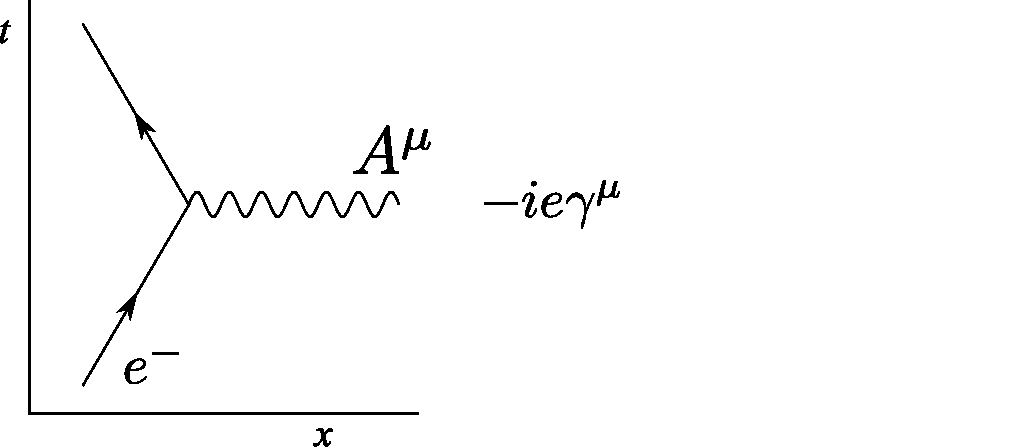
\includegraphics{feynmanruleqed} % in feynmanrules.svf as a Layer
  \caption{Feynman rule for QED}
  \label{fig:feynmanruleqed}
\end{figure}

La repulsión electromagnética esta representada por la figura \ref{fig:qedrepulsion}. En la Figura (a) el primer electrón emite un fotón y se dispersa, mientras que el segundo absorbe el fotón y se dispersa en la dirección opuesta. En la Figura (b) el primer electón absorve el fotón emitido por el segundo electrón. Los dos diagrams se representa por uno único con el fotón en horizontal como se muestra en la Figura (c).

\begin{figure}
  \centering
  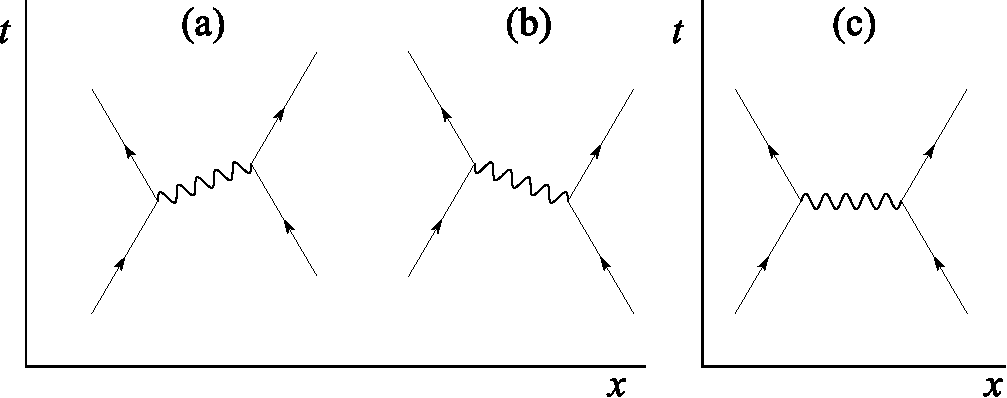
\includegraphics{qedrepulsion}
  \caption{Electromagnetic repulsion. The diagrams (a) and (b) are summarized in the diagram (c)}
  \label{fig:qedrepulsion}
\end{figure}


%Intentando obtener el operador Hamiltoniano y demás:
%  \begin{align}
%   T^\mu_\nu=&\frac{\partial\mathcal{L}}{\partial\left(\partial_\mu\psi\right)}\partial_\nu\psi+\partial_\nu\bar{\psi}\frac{\partial\mathcal{L}}{\partial\left(\partial_\mu\bar{\psi}\right)}-\mathcal{L}\delta^\mu_\nu\nonumber\\
%   =&i\bar{\psi}\gamma^\mu\partial_\nu\psi-\mathcal{L}\delta^\mu_\nu\,.
% \end{align}
% La expresión para $T^0_i$ es la misma que antes
% \begin{align}
%   T^0_0=i\psi^\dagger\partial_0\psi-i\psi^\dagger\partial_0\psi-i\psi^\dagger\gamma^0\gamma^i\partial_i\psi+m\psi^\dagger\psi-eQ\bar{\psi}\gamma^\mu\psi A_\mu +\tfrac{1}{4}F^{\mu\nu}F_{\mu\nu}.
% \end{align}



\section{Cromodinámica Cuántica}
\label{sec:inter-fuert}
Los protones, neutrones, piones, kaones y demás hadrones, son partículas compuestas de constituyentes elementales llamados quarks. Por ejemplo los protones, neutrones y piones están constituidos de quarks up y down. Los hadrones están dividos en  bariones, $B$, constituidos de tres quarks, y los mesones, $M$, de dos. Para satisfacer el principio de exclusión de Pauli, y justificar el confinamiento de los hadrones, se requiere que cada quark contenga $N_c$ cargas diferentes, llamadas cargas de color, de manera que la carga de color de un hadrón sea cero. Muchos resultados experimentales respaldan la existencia de tres cargas de color para cada quark, $N_c=3$. De este modo cada quark $q=u,d,c,s,t,b$ viene en tres colores
\begin{equation}
  q_\alpha=q_1,q_2,q_3=q_r,q_b,q_g,
\end{equation}
donde los últimos subíndices hacen referencia a los colores red, blue, green. De este modo los Bariones y mesones están descritos por combinaciones singletes de color del tipo $q_r q_b q_g$ y $q_r\bar{q}_r$,
\begin{equation}
\label{eq:199qft}
  B=\frac{1}{\sqrt{6}}\epsilon_{\alpha\beta\gamma}
  \left|q_\alpha q_\beta q_\gamma\right\rangle \qquad M=\frac{1}{\sqrt{3}}\delta^{\alpha\beta}\left|\bar{q}_{\alpha}q_\beta\right\rangle
\end{equation}
Estos estados son singletes de color.
Una de las determinaciones de $N_c$ proviene del observable
\begin{align}
  R\approx&\frac{\sigma(e^+e^-\to\text{hadrones})}{\sigma(e^+e^-\to\mu^+\mu^-)}
\end{align}

Para $f=u,d,s,c,b,t$, (en orden de masa) tenemos que para una energía donde se pueden producir hadrones compuestos de hasta  quarks $f_{\text{max}}$
\begin{align}
  R\approx&\frac{\sum_{f=u}^{f_{\text{max}}}\sum_{\alpha=1}^{N_c}\sigma(e^+e^-\to f_\alpha\bar{f}_\alpha)}{\sigma(e^+e^-\to\mu^+\mu^-)}\nonumber\\
  R\approx&N_c\frac{\sum_{f=u}^{f_{\text{max}}}\sigma(e^+e^-\to f\bar{f})}{\sigma(e^+e^-\to\mu^+\mu^-)}
\end{align}
De este modo $R$ esta dado por la suma de las cargas eléctricas al cuadrado
\begin{align}
\label{eq:254qft}
R\approx&N_c\frac{\sum_f Q_f^2}{Q_\mu^2}\nonumber\\
=&N_c\sum_{f=u}^{f_{\text{max}}} Q_f^2\nonumber\\
=&
\begin{cases}
  N_c[(\frac{2}{3})^2+2(\frac{-1}{3})^2]=\frac{2}{3}N_c&f=u,d,s,\;f_{\text{max}}=s\\
  N_c[2(\frac{2}{3})^2+2(\frac{-1}{3})^2]=\frac{10}{9}N_c&f_{\text{max}}=c\\
  N_c[2(\frac{2}{3})^2+3(\frac{-1}{3})^2]=\frac{11}{9}N_c&f_{\text{max}}=b
\end{cases}\nonumber\\
=&
\begin{cases}
  2&N_c=3,\qquad f_{\text{max}}=s\\
  \frac{10}{3}&N_c=3,\qquad f_{\text{max}}=c\\
  \frac{11}{3}&N_c=3,\qquad f_{\text{max}}=b\\
\end{cases}
\end{align}
%\left(\right)
En la figura, tomada de \cite{a}, se muestra el gráfico de $R$ con respecto a $\sqrt{s}$ (la energía de centro de masa de la colisión). Se observan dos escalones, uno que va hasta una energía $\sqrt{s}\approx4\,$GeV que corresponden a $f=u,d,s$, con un $R\approx2$,  y otro hasta $\sqrt{s}\approx40\,$GeV que corresponde a $f=u,d,s,c,b$, con un $R\approx3.7\approx11/3$. Los dos valores de $R$ son compatibles con los esperados de la ec.~\eqref{eq:254qft}. Como referencia también se señalan los valores para $N_c=4$ (en rojo). 
\begin{figure}
  \centering
  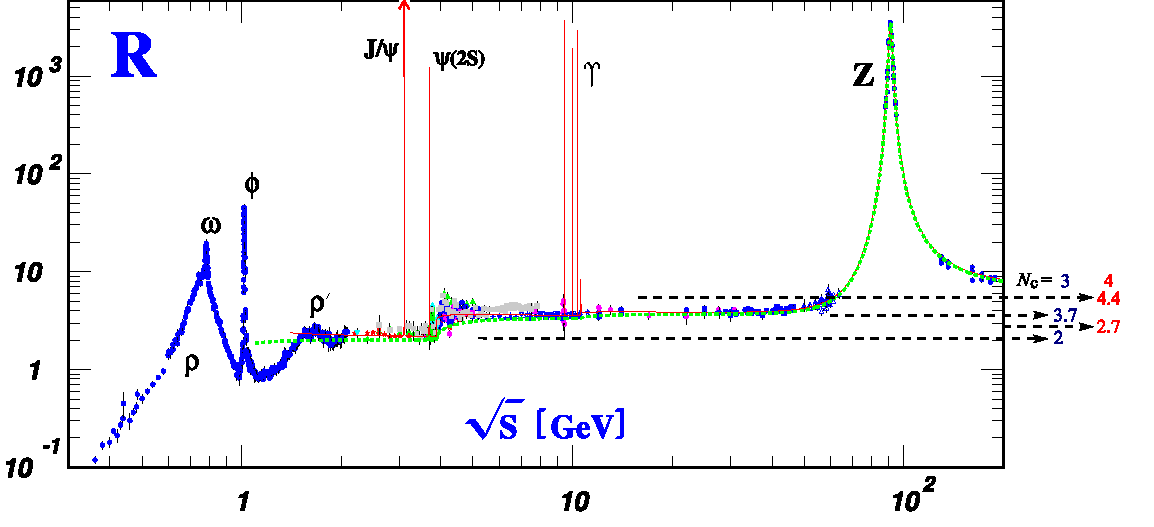
\includegraphics[scale=0.9]{r}
  \caption{Datos para $R$}
  \label{fig:r}
\end{figure}

Si queremos que el color sea una carga conservada como la carga eléctrica, ésta debe ser la consecuencia de una simetría gauge local. Para tener tres cargas diferentes la posibilidad más simple es imponer la simetría $SU(3)_c$, tal que tengamos un vector compuesto de 3 espinores de Dirac en el espacio de color:
\begin{equation}
  \Psi=
  \begin{pmatrix}
    \psi_r\\
    \psi_b\\
    \psi_g
  \end{pmatrix}
  =
  \begin{pmatrix}
    q_r\\
    q_b\\
    q_g
  \end{pmatrix}.
\end{equation}
El Lagrangiano de Dirac con invarianza gauge global $SU(3)$, para un quark, se puede escribir como
\begin{equation}
  \label{eq:128qft}
  \mathcal{L}_{\text{global}}=i\bar{\Psi}\gamma^\mu\partial_\mu\Psi-m\bar{\Psi}\Psi,
\end{equation}
donde
\begin{equation}
  \Psi\to \Psi'=\exp\left(i\theta_a\frac{\lambda^a}{2}\right)\Psi.
\end{equation}
$a=1,\ldots,8$, $\lambda_a/2$ son los ocho generadores de $SU(3)$ y $\theta_a$ son los parámetros de la transformación global. Los generadores de $SU(3)$
\begin{align}
  \Lambda^a\equiv\frac{\lambda^a}{2}\,,
\end{align}
satisfacen el álgebra
\begin{equation}
  \left[\frac{\lambda^a}{2},\frac{\lambda^b}{2}\right]=if^{abc}\frac{\lambda^c}{2}\,,
\end{equation}
donde $f^{abc}$ son las constantes de estructura fina de $SU(3)$.

En un análisis similar al de la sección \ref{sec:diracs-lagrangian} tenemos que la Acción invariante gauge local bajo $SU(3)_c$, se obtiene de reemplazar la derivada normal por la derivada covariante 
\begin{equation}
  \label{eq:127qft}
  \mathcal{L}_{\text{local}}=i\bar{\Psi}\gamma^\mu\mathcal{D}_\mu\Psi-m\bar{\Psi}\Psi
  -\frac{1}{2}\operatorname{Tr}\left({G}^{\mu\nu}{G}_{\mu\nu}\right),
\end{equation}
donde
\begin{align}
  \label{eq:qcdtr}
  \Psi\to \Psi'&=U(x)\Psi\nonumber\\
  \mathcal{D}_\mu\Psi\to \left(\mathcal{D}_\mu\Psi\right)'&
  =U(x)\mathcal{D}_\mu\Psi,
\end{align}
con la matriz $3\timesm 3$
\begin{align}
  U(x)=\exp\left[i\theta_a(x)\frac{\lambda^a}{2}\right]\,,
\end{align}
y
\begin{equation}
  \mathcal{D}_\mu=\partial_\mu-i g_s\frac{\lambda_a}{2}G_\mu^a\equiv\partial_\mu-i g_s {G}_\mu
\end{equation}
donde hemos definido la matriz $3\timesm 3$  $G_\mu$, como
\begin{equation}
  \left({G}_\mu\right)_{\alpha\beta}=\left(\frac{\lambda_a}{2}\right)_{\alpha\beta}G_\mu^a
\end{equation}

Este Lagrangiano da lugar a la interacción fuerte y es llamado el Lagrangiano de la Cromodinámica Cuántica, o el Lagrangiano de la QCD de sus siglas en Inglés.

De \eqref{eq:qcdtr}, tenemos
\begin{align}
   \mathcal{D}_\mu\Psi\to \left(\mathcal{D}_\mu\Psi\right)'=&\mathcal{D}'_\mu\Psi'
  =U(x)\mathcal{D}_\mu\Psi\nonumber\\
\mathcal{D}'_\mu U\Psi
  =U(x)\mathcal{D}_\mu\Psi\,.
\end{align}
Por consiguiente
\begin{equation}
  {\mathcal{D}'}^\mu U=U\mathcal{D}^\mu
\end{equation}
\begin{equation}
  \mathcal{D}^\mu\to\left(
    \mathcal{D}^\mu
  \right)'=U\mathcal{D}^\mu U^{-1}
\end{equation}
\begin{align}
  \label{eq:251qft}
   {\mathcal{D}}^\mu\psi\to{\left({\mathcal{D}}^\mu\psi\right)}'=
  (\partial^\mu-i g_s {G'}^\mu) U\psi=&U(\partial^\mu-i g_s {G}^\mu\mathcal{D})\psi\nonumber\\
  U\partial^\mu\psi+(\partial^\mu U)\psi-i g_s {G'}^\mu U \psi=&U\partial^\mu\phi-i g_s {G}^\mu \psi\nonumber\\
  (\partial^\mu U)\psi-i g_s {G'}^\mu U \psi=&-i g_s U {G}^\mu \psi\nonumber\\
  -i g_s {G'}^\mu U \psi=&-(\partial^\mu U)\psi-i g_s U {G}^\mu \psi\,,
\end{align}
de modo que
\begin{align}
     {G'}^\mu U =&\frac{1}{i g_s}(\partial^\mu U)+ U{G}^\mu \nonumber\\
   {G'}^\mu  =&-\frac{i}{g_s}(\partial^\mu U)U^{-1}+ U{G}^\mu U^{-1}\,.
\end{align}
Como $U$ es unitaria, la transformación de los campos gauge puede escribirse como
\begin{equation}
    {G}^\mu\to\left({G}^\mu\right)'=U{G}^\mu U^{-1}-\frac{i}{g_s}\left(\partial^\mu U\right)U^\dagger.
\end{equation}

Entonces
\begin{align}
\label{eq:Gmuinv}
  \Lambda^a{G'}^\mu_a\approx&(1+i\theta_b\Lambda^b)\Lambda^cG^\mu_c(1-i\theta_d\Lambda^d)-\frac{i}{g_s}[i(\partial^\mu\theta_e)\Lambda^e(1-i\theta_f\Lambda^f)]\nonumber\\
  =&(\Lambda^c+i\theta_b\Lambda^b\Lambda^c)(1-i\theta_d\Lambda^d)G^\mu_c-\frac{i}{g_s}[i(\partial^\mu\theta_e)\Lambda^e(1-i\theta_f\Lambda^f)]\nonumber\\
  \approx&[\Lambda^c-i\theta_d\Lambda^c\Lambda^d+i\theta_b\Lambda^b\Lambda^c]G^\mu_c+\frac{1}{g_s}\Lambda^e\partial^\mu\theta_e\nonumber\\
  =&[\Lambda^c-i\theta_b(\Lambda^c\Lambda^b-\Lambda^b\Lambda^c)]G^\mu_c+\frac{1}{g_s}\Lambda^e\partial^\mu\theta_e\nonumber\\
  =&\Lambda^aG^\mu_a-i(i f^{acb}\Lambda^a)G^\mu_c\theta_b+\frac{1}{g_s}\Lambda^a\partial^\mu\theta_a\nonumber\\
  =&\Lambda^a\left(G^\mu_a+\frac{1}{g_s}\partial^\mu\theta_a+f^{acb}G^\mu_c\theta_b\right)
\end{align}

de donde
\begin{align}
  \label{eq:gmutrinf}
  G^\mu_a\to {G'}^\mu_a\approx&G^\mu_a+\frac{1}{g_s}\partial^\mu\theta_a+f^{abc}G^\mu_b\theta_c
\end{align}
que se reduce al caso Abeliano cuando las constates de estructura son cero. Como era de esperarse cada campo gauge tiene asociado un parámetro de transformación gauge $\theta_a(x)$.




Similarmente, definiendo la matriz $3\timesm 3$, 
\begin{align}
  \label{eq:gmunu}
  {{G}}^{\mu\nu}&=\frac{i}{g_s}[\mathcal{D}^\mu,\mathcal{D}^\nu]\equiv\frac{\lambda_a}{2}G^{\mu\nu}_a,
\end{align}
tenemos
\begin{align}
  \label{eq:164qft}
   {G}^{\mu\nu}\psi =&\frac{i}{g_s}[\partial^\mu-ig_sG^\mu,\partial^\nu-ig_sG^\nu]\psi\nonumber\\
  =&\frac{i}{g_s}\left[\left(\partial^\mu-ig_sG^\mu\right)\left(\partial^\nu-ig_sG^\nu\right)\psi
    -\left(\partial^\nu-ig_sG^\nu\right)\left(\partial^\mu-ig_sG^\mu\right)\psi\right]\nonumber\\
  =&\frac{i}{g_s}\left\{\partial^\mu\partial^\nu\psi-g_s^2G^\mu G^\nu\psi-ig_s[\partial^\mu(G^\nu\psi)+G^\mu\partial^\nu\psi]
    -\partial^\nu\partial^\mu\psi+g_s^2G^\nu G^\mu\psi+ig_s[\partial^\nu(G^\mu\psi)+G^\nu\partial^\mu\psi]\right\}\nonumber\\
  =&\frac{i}{g_s}\{(\partial^\mu\partial^\nu-\partial^\nu\partial^\mu)\psi-g_s^2(G^\mu G^\nu-G^\nu G^\mu)\psi
  -ig_s[(\partial^\mu G^\nu)-(\partial^\nu G^\mu)]\psi\nonumber\\
  &-ig_s[G^\nu\partial^\mu\psi+G^\mu\partial^\nu\psi-G^\mu\partial^\nu\psi+G^\nu\partial^\mu\psi]\}\nonumber\\
=&[\partial^\mu G^\nu-\partial^\nu G^\mu-ig_s(G^\mu G^\nu-G^\nu G^\mu)]\psi\nonumber\\
=&\{\partial^\mu G^\nu-\partial^\nu G^\mu-ig_s[G^\mu,G^\nu]\}\psi
\end{align}

De modo que
\begin{align}
  {G}^{\mu\nu}=&\partial^\mu G^\nu-\partial^\nu G^\mu-ig_s[G^\mu,G^\nu]\,,
\end{align}
que se reduce al caso Abeliano cuando los bosones gauge conmutan. En términos de componentes
\begin{align}
  \Lambda^a{G}^{\mu\nu}_a=&\Lambda^a\partial^\mu G^\nu_a-\Lambda^a\partial^\nu G^\mu_a-ig_s[\Lambda^bG^\mu_b,\Lambda^cG^\nu_c]\nonumber\\
  =&\Lambda^a\partial^\mu G^\nu_a-\Lambda^a\partial^\nu G^\mu_a-ig_s[\Lambda^b,\Lambda^c]G^\mu_bG^\nu_c\nonumber\\
  =&\Lambda^a\partial^\mu G^\nu_a-\Lambda^a\partial^\nu G^\mu_a-ig_s(i\Lambda^af_{a b c})G^\mu_bG^\nu_c\nonumber\\
  =&\Lambda^a\partial^\mu G^\nu_a-\Lambda^a\partial^\nu G^\mu_a+\Lambda^ag_sf_{a b c}G^\mu_bG^\nu_c\,.
\end{align}
Por consiguiente
\begin{equation}
  \label{eq:258qft}
  G^{\mu\nu}_a=\partial^\mu G^\nu_a-\partial^\nu G^\mu_a+g_s f^{abc}G^\mu_b G^\nu_c\equiv\widetilde{G}^{\mu\nu}_a+g_s f^{abc}G^\mu_b G^\nu_c,
\end{equation}
con
\begin{equation}
  \widetilde{G}^{\mu\nu}_a=\partial^\mu G^\nu_a-\partial^\nu G^\mu_a
\end{equation}



A diferencia del caso Abeliano $G^{\mu\nu}$ ya no es invariante bajo transformaciones gauge
\begin{align}
G^{\mu\nu}\to    {G'}^{\mu\nu}
  &=\frac{i}{g_s}\left[{\mathcal{D}'}^\mu,{\mathcal{D}'}^\nu\right]\nonumber\\
&=\frac{i}{g_s}\left[U{\mathcal{D}}^\mu U^{-1},U{\mathcal{D}}^\nu U^{-1}\right]\nonumber\\
&=U{{G}}^{\mu\nu}U^{-1}\,.
\end{align}

Note que con la definición \eqref{eq:gmunu}, la derivada covariante de la matrix $G^{\mu\nu}$, transforma como la matrix $G^{\mu\nu}$
\begin{align}
\mathcal{D}_\mu G^{\mu\nu} \to\left(\mathcal{D}_\mu G^{\mu\nu}\right)'=U\mathcal{D}_\mu G^{\mu\nu} U^{-1}\,.
\end{align}


Para poder obtener un invariante bajo transformaciones gauge a partir del producto $G^{\mu\nu}G_{\mu\nu}$, debemos utilizar la traza 
\begin{align}
  \operatorname{Tr}\left(G^{\mu\nu}G_{\mu\nu}\right)\to
  \operatorname{Tr}\left({G\,'}^{\mu\nu}{G\,'}_{\mu\nu}\right)
  =&\operatorname{Tr}\left(U{{G}}^{\mu\nu}U^{-1}U{{G}}_{\mu\nu}U^{-1}\right)\nonumber\\
  =&\operatorname{Tr}\left(U{{G}}^{\mu\nu}{{G}}_{\mu\nu}U^{-1}\right)\nonumber\\
  =&\operatorname{Tr}\left(U^{-1}U{{G}}^{\mu\nu}{{G}}_{\mu\nu}\right)\nonumber\\
  =&\operatorname{Tr}\left({{G}}^{\mu\nu}{{G}}_{\mu\nu}\right)\,.
\end{align}
Teniendo en cuenta la normalización de las matrices de Gell-Man
\begin{align}
  \operatorname{Tr}\left(\lambda^a\lambda^b\right)=&2\delta^{ab}\nonumber\\
  \operatorname{Tr}\left(\Lambda^a\Lambda^b\right)=&\frac{1}{2}\delta^{ab}\,,
\end{align}
tenemos (suma sobre indices repetidos de $SU(3)$)
\begin{align}
  \operatorname{Tr}\left(G^{\mu\nu}G_{\mu\nu}\right)\to
  \operatorname{Tr}\left({G\,'}^{\mu\nu}{G\,'}_{\mu\nu}\right)
  =&\operatorname{Tr}\left(\Lambda^a{G}^{\mu\nu}_a \Lambda^b{G}_{\mu\nu}^b\right)\nonumber\\
  =&\operatorname{Tr}\left(\Lambda^a \Lambda^b\right){G}^{\mu\nu}_a {G}_{\mu\nu}^b\nonumber\\
  =&\frac{1}{2}\delta^{a b}{G}^{\mu\nu}_a {G}_{\mu\nu}^b\nonumber\\
  =&\frac{1}{2}{G}^{\mu\nu}_a {G}_{\mu\nu}^a\,.
\end{align}

Expandiendo el Lagrangiano en ec.~(\ref{eq:127qft}), tenemos
\begin{align}
  \mathcal{L}=&i\bar{\Psi}\gamma^\mu\left(\partial_\mu-i g_s\frac{\lambda_a}{2}G_\mu^a\right)\Psi
  -m\bar{\Psi}\Psi- \frac{1}{2}\operatorname{Tr}\left(G^{\mu\nu} G_{\mu\nu}\right)\nonumber\\
  =&i\bar{\Psi}\gamma^\mu\left(\partial_\mu-i g_s\frac{\lambda_a}{2}G_\mu^a\right)\Psi
  -m\bar{\Psi}\Psi- \frac{1}{4}G^{\mu\nu}_a G_{\mu\nu}^a\nonumber\\
=&i\bar{\Psi}\gamma^\mu\partial_\mu\Psi-m\bar{\Psi}\Psi+g_s\bar{\Psi}\gamma^\mu\frac{\lambda_a}{2}G_\mu^a\Psi
  - \frac{1}{4}G^{\mu\nu}_a G_{\mu\nu}^a\nonumber\\
=&i\bar{\Psi}\gamma^\mu\partial_\mu\Psi-m\bar{\Psi}\Psi+g_s\bar{\Psi}\gamma^\mu\frac{\lambda_a}{2}\Psi G_\mu^a
  - \frac{1}{4}\widetilde{G}^{\mu\nu}_a \widetilde{G}_{\mu\nu}^a\nonumber\\
  &- \frac{1}{4}\left(g_s\widetilde{G}^{\mu\nu}_af_{a d e}G^d_\mu G^e_\nu
    +g_sf^{a b c}G_b^\mu G_c^\nu\widetilde{G}_{\mu\nu}^a
    +g_s^2f^{a b c}f_{a d e}G_b^\mu G_c^\nu G^d_\mu G^e_\nu\right)\nonumber\\
=&\mathcal{L}_{\text{free}}+\mathcal{L}_{\text{gauge}}+\mathcal{L}_{\text{SI}}\,,
\end{align}
donde

\begin{align}
\label{eq:qcdgauge}
\mathcal{L}_{\text{free}}=&i\bar{\Psi}\gamma^\mu\partial_\mu\Psi-m\bar{\Psi}\Psi\nonumber\\
  \mathcal{L}_{\text{gauge}}=&g_s\bar{\Psi}\gamma^\mu\frac{\lambda_a}{2}\Psi G_\mu^a
  - \frac{1}{4}\widetilde{G}^{\mu\nu}_a \widetilde{G}_{\mu\nu}^a\nonumber\\
  \mathcal{L}_{\text{SI}}=&- \frac{1}{4}\left(g_s\widetilde{G}^{\mu\nu}_af_{a d e}G^d_\mu G^e_\nu
    +g_sf^{a b c}G_b^\mu G_c^\nu\widetilde{G}_{\mu\nu}^a
    +g_s^2f^{a b c}f_{a d e}G_b^\mu G_c^\nu G^d_\mu G^e_\nu\right)\,.
\end{align}

Hemos divido el Lagrangiano en tres partes
\begin{itemize}
\item El Lagrangiano libre de Dirac
\item Una parte gauge que puede escribirse como un Lagrangiano electromagnético:
\begin{align}
  \mathcal{L}_{\text{gauge}}=&-\frac{1}{4}\left(\partial^\mu G^\nu_a-\partial^\nu G^\mu_a\right)\left(\partial_\mu G_\nu^a-\partial_\nu G_\mu^a\right)-J^\nu_aG_\nu^a,
\end{align}
dende
\begin{align}
  J^\mu_a=-g_s\bar{\Psi}\gamma^\mu\frac{\lambda_a}{2}\Psi\,,
\end{align}
es la nueva corriente conservada de interacción fuerte que surge como consecuencia de la invarianza gauge local $SU(3)$; y 
\item Una parte de auto-interacciones gauge:
  \begin{align}
    \mathcal{L}_{\text{SI}}  &=- \frac{g_s}{2}f^{a b c}\widetilde{G}_{\mu\nu}^aG_b^\mu G_c^\nu
    +\frac{g_s^2}{4}f^{a b c}f_{a d e}G_b^\mu G_c^\nu G^d_\mu G^e_\nu\nonumber\\
  &=-\frac{g_s}{2}f^{abc}\left(\partial^\mu G^\nu_a-\partial^\nu G^\mu_a\right)G^b_\mu G^c_\nu-\frac{g_s^2}{4}f^{abc}f_{ade}G^\mu_bG^\nu_cG^d_\mu G^e_\nu.
  \end{align}
que se desaparecen en el caso Abeliano.
\end{itemize}

El Lagrangiano de interacción es:
\begin{align}
  \mathcal{L}_{\text{int}}=g_s\bar{\Psi}\gamma^\mu\frac{\lambda_a}{2}\Psi G_\mu^a-\frac{g_s}{2}f^{abc}\left(\partial^\mu G^\nu_a-\partial^\nu G^\mu_a\right)G^b_\mu G^c_\nu-\frac{g_s^2}{4}f^{abc}f_{ade}G^\mu_bG^\nu_cG^d_\mu G^e_\nu.
\end{align}

%ver la discusión en el libro de Feyman sobre QED

From \cite{Feynman:1986er} (pag 136):
\begin{quote}
  The quarks have an additional type of polarization that is not related to geometry. The idiot physicists, unable to come up with any wonderful Greek words anymore, call this type of polarization by the unfortunate name of ``color'', which has nothing to do with color in the nornal sense. At a particular time, a quark can be in one of three conditions, or ``colors''--R, G, or B (can you guess what they stand for?). A quark's ``color'' can be changed when the quarl emits or absorbs a gluon. The gluons comw in eigth diffent types, according to the ``colors'' they can couple with. For example, if a red quark changes to green, it emits a red-antigreen gluon--a gluon that takes the red from quark and gives it green (``antigreen'' means the gluon is carrying green in the opposite direction). This gluon could be absorved by a grren quark, which changes to red (see Fig.~\ref{fig:qcd}). There are eigth different possible gluons, such as red-antired, red-antiblue, red-antigrren, and so on (you'd think there'd be nine, but for technical reasons, onw is missing)\footnote{
    \begin{align*}
      \begin{pmatrix}
        r\bar{r} & r\bar{b} r\bar{g}\\ 
        b\bar{r} & b\bar{b} b\bar{g}\\ 
        g\bar{r} & g\bar{b} g\bar{g}\\ 
      \end{pmatrix},\qquad\text{with}\quad r\bar{r}+b\bar{b}+g\bar{g}=0
    \end{align*}
}. The theory is not very complicated.  The complete rule of gluons is: gluons couople with things having ``color''--it just requires a little bookkeeping to keep track of where the ``colors go''.  There is, however, an interesesting possibility created by this rule: gluons can couple with other gluons (see Fig.~\ref{fig:qcd3gluon}).
\end{quote}

%11 12 13
%21 22 23
%31 32 33
%33+11+22=0

El primer término da lugar a interacciones de cambio de color de quarks como la que se ilustra en la Figura \ref{fig:qcd}
\begin{figure}
  \centering
  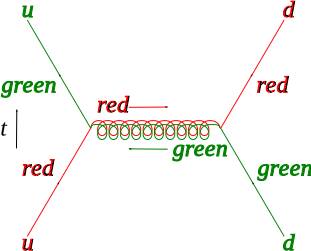
\includegraphics{qcd} % In qcd.svg as a layer
  \caption{Quark--gluon interaction}
  \label{fig:qcd}
\end{figure}

Mientras que el segundo término da lugar a autointeracciones de los gluones como se muestra en la Figura \ref{fig:qcd3gluon}
\begin{figure}
  \centering
  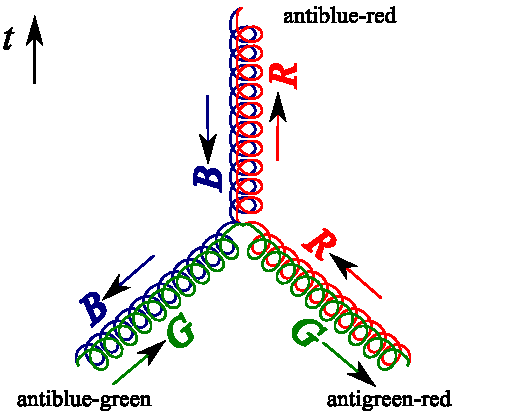
\includegraphics{qcd3gluon}% In qcd.svg as a layer
  \caption{Triple--gluon self--interaction. The anticolors are the colors running back in time.}
  \label{fig:qcd3gluon}
\end{figure}


Todas las interacciones están determinadas en términos de una única constante de acoplamiento $g_s$. Las autointeracciones gauge pueden explicar aspectos de la interacción fuerte como la libertada asintótica, que consiste en que las interacciones fuertes se vuelven más débiles a distancias cortas. 

En términos de índices de color la corriente, y las otras partes del Lagrangiano, pueden escribirse como
\begin{equation}
  \label{eq:223qft}
  J^\mu_a=-g_s\bar{q}^\alpha\gamma^\mu q^\beta\left(\frac{\lambda_a}{2}\right)_{\alpha\beta}.
\end{equation}
Note que tanto para la Electrodinámica Cuántica como para la Cromodinámica Cuántica la corriente $\bar{\psi}\Gamma\psi$ es vectorial. Para las interacciones débiles la estructura es más complicada y requiere un conocimiento más profundo de la ecuación de Dirac y sus soluciones.

\subsection{Ecuaciones de Euler--Lagrange}
\label{sec:ecuaciones-de-euler-1}
Sigiendo los mismos procedimientos anteriores debemos llegar a los siguientes resultados. Para el campo $\Psi$
\begin{align}
  (i\gamma^\mu\mathcal{D}_\mu-m)\Psi=0\,,
\end{align}
\begin{align}
  &\partial_\mu\left[\frac{\partial\mathcal{L}}{\partial\left(\partial_\mu G_\nu^a\right)}\right]-\frac{\partial\mathcal{L}}{\partial G_\nu^a}\nonumber\\
=&\partial_\mu\left\{-  \widetilde{G}^{\mu\nu}_a-\frac{1}{2}g_s f_{dbc}G_b^\rho G^\sigma_c\frac{\partial}{\partial\left(\partial_\mu G_\nu^a\right)}
\left(\partial_\rho G_\sigma^d-\partial_\sigma G_\rho^d\right)\right\}
-g_s\overline{\Psi}\gamma^\nu\frac{\lambda_a}{2}\Psi\nonumber\\
&+\frac{g_s}{2} f^{dbc}\widetilde{G}^{\rho\sigma}_d(\delta_{\rho\nu}\delta_{ba}G^c_\sigma+G^b_\rho\delta_{\sigma\nu}\delta_{ca})
+\frac{g_s}{4}f^{ibc}f_{ide}(g^{\rho\alpha}g^{\sigma\beta}G^b_{\alpha}G^c_\beta G^d_\rho G^e_\sigma)\nonumber\\
  =&\partial_\mu\left\{- \widetilde{G}^{\mu\nu}_a-\frac{1}{2}g_s f_{dbc}G_b^\rho G^\sigma_c
\left(\delta_{\rho\mu}\delta_{\sigma\nu}\delta_{da}-\delta_{\sigma\mu}\delta_{\rho\nu}\delta_{da}\right)\right\}
-g_s\overline{\Psi}\gamma^\nu\frac{\lambda_a}{2}\Psi\nonumber\\
&+\frac{g_s}{2} f^{dac}\widetilde{G}^{\nu\sigma}_dG^c_\sigma
+\frac{g_s}{2} f^{dba}\widetilde{G}^{\rho\nu}_dG^b_\rho\nonumber\\
&+\frac{g_s}{4}f^{ibc}f_{ide}g^{\rho\alpha}g^{\sigma\beta}(\delta_{\alpha\nu}\delta_{ba}G^c_\beta G^d_\rho G^e_\sigma+G^b_{\alpha}\delta_{\beta\nu}\delta_{ca}G^d_\rho G^e_\sigma+G^b_{\alpha}G^c_\beta\delta_{\rho\nu}\delta_{da}G^e_\sigma+G^b_{\alpha}G^c_\beta G^d_\rho\delta_{\sigma\nu}\delta_{ea})\nonumber\\
  =&-\partial_\mu\left\{  \widetilde{G}^{\mu\nu}_a-\frac{1}{2}g_s f^{abc}G_b^\mu G^\nu_c
+\frac{1}{2}g_s f_{abc}G_b^\nu G^\mu_c\right\}
-g_s\overline{\Psi}\gamma^\nu\frac{\lambda_a}{2}\Psi\nonumber\\
&-\frac{g_s}{2} f^{adc}\widetilde{G}^{\nu\sigma}_dG^c_\sigma
-\frac{g_s}{2} f^{adb}\widetilde{G}^{\nu\rho}_dG^b_\rho\nonumber\\
&+\frac{g_s}{4}f^{iac}f_{ide}g^{\rho\nu}g^{\sigma\beta}G^c_\beta G^d_\rho G^e_\sigma
+\frac{g_s}{4}f^{iba}f_{ide}g^{\rho\alpha}g^{\sigma\nu}G^b_{\alpha}G^d_\rho G^e_\sigma
+\frac{g_s}{4}f^{ibc}f_{iae}g^{\nu\alpha}g^{\sigma\beta}G^b_{\alpha}G^c_\beta G^e_\sigma\nonumber\\
&+\frac{g_s}{4}f^{ibc}f_{ida}g^{\rho\alpha}g^{\nu\beta}G^b_{\alpha}G^c_\beta G^d_\rho\,.
\end{align}
Desarrollando los cuatro últimos términos, tenemos

\begin{align}
  &\frac{g_s}{4}f^{iac}f_{ide}g^{\rho\nu}g^{\sigma\beta}G^c_\beta G^d_\rho G^e_\sigma
+\frac{g_s}{4}f^{iba}f_{ide}g^{\rho\alpha}g^{\sigma\nu}G^b_{\alpha}G^d_\rho G^e_\sigma
+\frac{g_s}{4}f^{ibc}f_{iae}g^{\nu\alpha}g^{\sigma\beta}G^b_{\alpha}G^c_\beta G^e_\sigma\nonumber\\
&+\frac{g_s}{4}f^{ibc}f_{ida}g^{\rho\alpha}g^{\nu\beta}G^b_{\alpha}G^c_\beta G^d_\rho\nonumber\\
=&\frac{g_s}{4}f^{iac}f_{ide}G_d^\nu G_c^\mu G^e_\mu
+\frac{g_s}{4}f^{iba}f_{ide}G_e^\nu G_b^{\mu}G^d_\mu
+\frac{g_s}{4}f^{ibc}f_{iae}G_b^{\nu}G_c^\mu G^e_\mu
+\frac{g_s}{4}f^{ibc}f_{ida}G_c^\nu G_b^{\mu}G^d_\mu\nonumber\\
=&  \frac{g_s}{4}f^{dac}f_{dje}G_j^\nu G_c^\mu G^e_\mu
+\frac{g_s}{4}f^{dca}f_{dje}G_e^\nu G_c^{\mu}G^j_\mu
+\frac{g_s}{4}f^{dbc}f_{dae}G_b^{\nu}G_c^\mu G^e_\mu
+\frac{g_s}{4}f^{dbc}f_{dea}G_c^\nu G_b^{\mu}G^e_\mu\nonumber\\
=&  \frac{g_s}{4}f^{dac}f_{dje}G_j^\nu G_c^\mu G^e_\mu
+\frac{g_s}{4}f^{dca}f_{dje}G_e^\nu G_c^{\mu}G^j_\mu
+\frac{g_s}{4}f_{dac}f^{dje}G_j^{\nu}Gc_e^\mu G^c_\mu
+\frac{g_s}{4}f_{dca}f^{dje}G_e^\nu G_j^{\mu}G^c_\mu\nonumber\\
=&  -\frac{g_s}{4}f^{abc}G^b_\mu f_{cej}G_e^\mu G_j^\nu
-\frac{g_s}{4}f^{abc}G^b_{\mu}f_{cej}G_e^\mu G_j^\nu
-\frac{g_s}{4}f_{abc}G^b_\mu f^{cej}G_e^\mu G_j^{\nu}
-\frac{g_s}{4}f_{abc}G^b_\mu f^{cej}G_e^{\mu}G_j^\nu\nonumber\\
=&-g_sf_{abc}G^b_\mu f^{cej}G_e^{\mu}G_j^\nu
\end{align}
Entonces
\begin{align}
    &\partial_\mu\left[\frac{\partial\mathcal{L}}{\partial\left(\partial_\mu G_\nu^a\right)}\right]-\frac{\partial\mathcal{L}}{\partial G_\nu^a}\nonumber\\
    =&\partial_\mu\left(-  \widetilde{G}^{\mu\nu}_a-g_s f^{abc}G_b^\mu G^\nu_c
\right)
-g_s\overline{\Psi}\gamma^\nu\frac{\lambda_a}{2}\Psi
-g_s f^{acd}G^c_\mu\widetilde{G}^{\mu\nu}_d
-g_sf_{acd}G^c_\mu f^{dej}G_e^{\mu}G_j^\nu\nonumber\\
      =&-\partial_\mu{G}^{\mu\nu}_a-g_s f^{acd}G^c_\mu{G}^{\mu\nu}_d
-g_s\overline{\Psi}\gamma^\nu\frac{\lambda_a}{2}\Psi=0\,.
\end{align}
Entonces las Ecuaciones de Euler Lagrange para $G_\nu^a$, son
\begin{align}
\label{eq:Gmuael}
\partial_\mu{G}^{\mu\nu}_a+g_s f^{acd}G^c_\mu{G}^{\mu\nu}_d
=-g_s\overline{\Psi}\gamma^\nu\frac{\lambda_a}{2}\Psi\,.
\end{align}
Definiendo
\begin{align}
J^\mu_a = -g_s\bar{\Psi}\gamma^\mu\frac{\lambda_a}{2}\Psi\,,
\end{align}

La ec.\eqref{eq:Gmuael} puede reescribirse como:
\begin{align}
  \partial_\mu G^{\mu\nu}_a=-g_s\left[f_{abc}G^b_\mu G^{\mu\nu}_c+\bar{\Psi}\gamma^\nu\frac{\lambda_a}{2}\Psi  \right]
\end{align}
y usando el hecho que $\partial_\mu\partial_\nu=\partial_\nu\partial_\mu$:
\begin{align}
  \partial_\nu\partial_\mu G^{\mu\nu}_a=&\partial_\nu\partial_\mu\widetilde{G}^{\mu\nu}+g_s\partial_\nu\partial_\mu\left(f_{abc}G^\mu_bG^\nu_c\right)\nonumber\\
=&0+\frac{1}{2}\left[g_s\partial_\nu\partial_\mu\left(f_{abc}G^\mu_bG^\nu_b\right)+g_s\partial_\nu\partial_\mu\left(f_{abc}G^\mu_bG^\nu_c\right)\right]\nonumber\\
=&\frac{1}{2}\left[g_s\partial_\nu\partial_\mu\left(f_{abc}G^\mu_bG^\nu_b\right)+g_s\partial_\mu\partial_\nu\left(f_{abc}G^\mu_bG^\nu_c\right)\right]\nonumber\\
=&\frac{1}{2}\left[g_s\partial_\nu\partial_\mu\left(f_{abc}G^\mu_bG^\nu_b\right)+g_s\partial_\nu\partial_\mu\left(f_{acb}G^\nu_cG^\mu_b\right)\right]\nonumber\\
=&\frac{1}{2}\left[g_s\partial_\nu\partial_\mu\left(f_{abc}G^\mu_bG^\nu_b\right)-g_s\partial_\mu\partial_\nu\left(f_{abc}G^\mu_bG^\nu_c\right)\right]\nonumber\\
=&0\,,
\end{align}
como en el caso Abeliano, tenemos la corriente conservada
\begin{align}
  \partial_\nu j^\nu=0\,,
\end{align}
donde
\begin{align}
\label{eq:jnuqcd}
  j^\nu_a=&-g_s\left[f_{abc}G^b_\mu G^{\mu\nu}_c+\bar{\Psi}\gamma^\nu\frac{\lambda_a}{2}\Psi  \right]\,.
\end{align}

El primer término corresponde a las autointeracciones y el segundo a la corriente de color generada por los quarks.


\subsection{Derivada covariante adjunta}
Toda el algebra de $SU(3)$ se puede escribir en notación vectorial en términos de vectores de 8 componentes asociados al espacio de los generadores de $SU(3)$. Este nos permitira entender como las autointeracciones gauge emergen también de la derivada covariante cuando se escribe en la representación adjunta de $SU(3)$.

Definiendo el producto vectorial de $SU(3)$ como
\begin{align}
  \left(\mathbf{A}\timesm \mathbf{B}\right)_a=f_{abc}A^b B^c\,,
\end{align}
si $\mathbf{G}^\mu$ es un vector en el espacio $SU(3)$ con las 8 componentes $G^\mu_a$, entonces podemos escribir \eqref{eq:gmutrinf} como
\begin{align}
  \mathbf{G}_\mu\to\mathbf{G}'_\mu=\mathbf{G}_\mu+\frac{1}{g_s}\partial_\mu\boldsymbol{\theta}+\mathbf{G}_\mu\timesm \boldsymbol{\theta}\,.
\end{align}

Podemos escribir también la ec.~\eqref{eq:258qft} en términos de vectores en el espacio $SU(3)$ como:
\begin{align}
  \mathbf{G}^{\mu\nu}=\partial^\mu \mathbf{G}^\nu-\partial^\nu \mathbf{G}^\mu+g_s \mathbf{G}^\mu\timesm  \mathbf{G}^\nu\,,
\end{align}
donde $\mathbf{G}^{\mu\nu}$ es el vector en el espacio $SU(3)$ con las 8 componentes $G^{\mu\nu}_a$.



De igual forma, podemos escribir \eqref{eq:Gmuael} en forma vectorial como
\begin{align}
  \partial_\mu\mathbf{G}^{\mu\nu}+g_s \mathbf{G}_\mu\timesm \mathbf{G}^{\mu\nu}=\mathbf{J}^\nu
\end{align}
y la corriente conservada como
\begin{align}
 \mathbf{j}^\nu =&-g_s\left[-\mathbf{G}^{\mu\nu}\timesm \mathbf{G}_\nu^b+\bar{\Psi}\gamma^\nu\frac{\boldsymbol{\lambda}}{2}\Psi  \right]\,.
\end{align}

Como ${G}^{\mu\nu}$ es una matrix $8\timesm 8$, su derivada covariante debe estar en la representación adjunta de $SU(3)$
\begin{align}
  \left(\Lambda^a\right)_{bc}=-i\left(f^a\right)_{bc}\,,
\end{align}
con
\begin{align}
  \left[\Lambda^a,\Lambda^b\right]=i f_{abc}\Lambda^c\,.
\end{align}
En esta representación la derivada covariante queda
\begin{align}
  \mathcal{D}_\mu=\partial_\mu-i g_s\Lambda_aG_\mu^a
\end{align}
En componentes
\begin{align}
  \left(\mathcal{D}_\mu\right)_{ab}=&\delta_{ab}\partial_\mu-i g_s (\Lambda^c)_{ab}G_\mu^c\nonumber\\
  =&\delta_{ab}\partial_\mu-g_s f_{cab}G_\mu^c\nonumber\\
  =&\delta_{ab}\partial_\mu+g_s f_{acb}G_\mu^c\,.
\end{align}

Aplicada sobre la componente $G^{\mu\nu}_b$, queda
\begin{align}
 \left(\mathcal{D}_\mu\right)_{ab}G^{\mu\nu}_b  =&\delta_{ab}\partial_\mu G^{\mu\nu}_b+g_s f_{acb}G_\mu^cG^{\mu\nu}_b\nonumber\\
 \left(\mathcal{D}_\mu\right)_{ab}G^{\mu\nu}_b  =&\partial_\mu G^{\mu\nu}_a+g_s \left(\mathbf{G}_\mu\timesm \mathbf{G}^{\mu\nu}\right)_a\nonumber\\
 \left(\mathcal{D}_\mu\mathbf{G}^{\mu\nu}\right)_a  =&\partial_\mu\mathbf{G}^{\mu\nu}_a+g_s \left(\mathbf{G}_\mu\timesm \mathbf{G}^{\mu\nu}\right)_a\,,
\end{align}
podemos escribir la derivada covariante de $\mathbf{G}^{\mu\nu}=\left(G^{\mu\nu}_1,\cdots,G^{\mu\nu}_8\right)$ como
\begin{align}
  \mathcal{D}_\mu \mathbf{G}^{\mu\nu}=&\partial_\mu\mathbf{G}^{\mu\nu}+g_s \mathbf{G}_\mu\timesm \mathbf{G}^{\mu\nu}\,.
\end{align}


Entonces las las Ecuaciones de Euler Lagrange para $G_{\mu\nu}^a$, en \eqref{eq:Gmuael} se pueden escribir como
\begin{align}
  \mathcal{D}_\mu \mathbf{G}^{\mu\nu}=&\mathbf{J}^\nu\,,
\end{align}
donde el vector en espacio $SU(3)$ $\mathbf{J}^\nu$, tiene por componentes
  \begin{align}
J^\mu_a = -g_s\bar{\Psi}\gamma^\mu\frac{\lambda_a}{2}\Psi\,.
\end{align}

Para escribir el Lagrangiano en forma vectorial en el espacio $SU(3)$, debemos reescribir la transformación gauge de $G_{\mu\nu}$ en términos de vectores de $SU(3)$. Como
\begin{align}
  {G}_{\mu\nu}\to{G}'_{\mu\nu}=&U G_{\mu\nu} U^{\dagger}\nonumber\\
  =&(1+i\theta_b\Lambda^b)\Lambda^cG^c_{\mu\nu}(1-i\theta_b\Lambda^b)
\end{align}
podemos realizar los mismos pasos que en \eqref{eq:Gmuinv}. El resultado es
\begin{align}
    G_{\mu\nu}^a\to {G'}_{\mu\nu}^a\approx&G_{\mu\nu}^a+f^{abc}G_{\mu\nu}^b\theta^c\,.
\end{align}
Note que en el caso Abeliano $f_{abc}=0$, el tensor correspondiente es invariante gauge, como ocurre el caso electromagnético. En notación de vectores de $SU(3)$:
\begin{align}
  \mathbf{G}_{\mu\nu}\to\mathbf{G}'_{\mu\nu}\approx\mathbf{G}_{\mu\nu}+\mathbf{G}_{\mu\nu}\timesm \boldsymbol{\theta}\,.
\end{align}
Utilizando la propiedad cíclica del triple producto escalar
\begin{align}
  \mathbf{A}\cdot(\mathbf{B}\timesm \mathbf{C})=\mathbf{B}\cdot(\mathbf{C}\timesm \mathbf{A})=\mathbf{C}\cdot(\mathbf{A}\timesm \mathbf{B})\,,
\end{align}
podemos construir el invariante

\begin{align}
  G^{\mu\nu}_aG^a_{\mu\nu}=\mathbf{G}^{\mu\nu}\cdot\mathbf{G}_{\mu\nu}\to{\mathbf{G}'}^{\mu\nu}\cdot\mathbf{G}'_{\mu\nu}\approx&
  \mathbf{G}^{\mu\nu}\cdot\mathbf{G}_{\mu\nu}+\mathbf{G}^{\mu\nu}\cdot\left(\mathbf{G}_{\mu\nu}\timesm \boldsymbol{\theta}\right)
+\left(\mathbf{G}^{\mu\nu}\timesm \boldsymbol{\theta}\right)\cdot\mathbf{G}_{\mu\nu}\nonumber\\
=&\mathbf{G}^{\mu\nu}\cdot\mathbf{G}_{\mu\nu}+\mathbf{G}_{\mu\nu}\cdot\left(\boldsymbol{\theta}\timesm \mathbf{G}^{\mu\nu}\right)
+\left(\mathbf{G}^{\mu\nu}\timesm \boldsymbol{\theta}\right)\cdot\mathbf{G}_{\mu\nu}\nonumber\\
=& \mathbf{G}^{\mu\nu}\cdot\mathbf{G}_{\mu\nu}-\left(\mathbf{G}^{\mu\nu}\timesm \boldsymbol{\theta}\right)\cdot\mathbf{G}_{\mu\nu}
+\left(\mathbf{G}^{\mu\nu}\timesm \boldsymbol{\theta}\right)\cdot\mathbf{G}_{\mu\nu}\nonumber\\
=&\mathbf{G}^{\mu\nu}\cdot\mathbf{G}_{\mu\nu}\,.
\end{align}

El Lagrangiano de la QCD escrito en forma de vectores de $SU(3)$ es
\begin{align}
  \mathcal{L}=i\bar{\Psi}\gamma^\mu\left(\partial_\mu-i g_s\frac{\boldsymbol{\lambda}}{2}\cdot\mathbf{G}_\mu\right)\Psi
  -m\bar{\Psi}\Psi- \frac{1}{4}\mathbf{G}^{\mu\nu}\cdot\mathbf{G}_{\mu\nu}\,.
\end{align}
El Lagrangiano para los campos gauge, el cual puede generalizarse para cualquier teoría $SU(N)$, es
\begin{align}
  \mathcal{L}_{\text{gluon}}=\mathcal{L}_{\text{gauge}}+\mathcal{L}_{\text{SI}}=- \frac{1}{4}\mathbf{G}^{\mu\nu}\cdot\mathbf{G}_{\mu\nu}-\mathbf{J}_\nu\cdot\mathbf{G}^\nu\,,
\end{align}
Da lugar la ecuaciones de Maxwell pero con la derivada normal reemplzada por la derivada covariante 
\begin{align}
  \mathcal{D}_\mu \mathbf{G}^{\mu\nu}=&\mathbf{J}^\nu\,,
\end{align}
donde
\begin{align}
    \mathcal{D}_\mu \mathbf{G}^{\mu\nu}=&\partial_\mu\mathbf{G}^{\mu\nu}+g_s \mathbf{G}_\mu\timesm \mathbf{G}^{\mu\nu}\,.
\end{align}
Note que en el caso Abeliano, $U(1)$, la derivada covariante del tensor de campo se reduce a la derivada normal de dicho tensor. El término extra en la derivada covariante da lugar a las autointeracciones de los campos gauge.

\begin{itemize}
\item \textbf{Ejercicio:}

Muestre que la derivada covariante de $\mathbf{G}^{\mu\nu}$, transforma como $\mathbf{G}^{\mu\nu}$.
\end{itemize}

% \begin{align}
%   \mathcal{D}_\mu G^{\mu\nu}=&\left(\partial_\mu-i g_s G_\mu\right)G^{\mu\nu}\nonumber\\
%   =&\partial_\mu G^{\mu\nu}-i g_s G_\mu G^{\mu\nu}\nonumber\\
%   =&\Lambda^a\partial_\mu G^{\mu\nu}_a-i g_s \Lambda_b\Lambda^cG_\mu^bG^{\mu\nu}_c
% \end{align}


\section{Spontaneous symmetry breaking}
\begin{frame}[fragile,allowframebreaks]
Escribamos el Lagrangiano para una partícula escalar real de masa $m$ como
\begin{equation}
\label{eq:83qft}
\mathcal{L}=\tfrac{1}{2}\partial^\mu\phi\partial_\mu\phi-V(\phi)
\end{equation}
con
\begin{equation}
  V(\phi)=\tfrac{1}{2}\mu^2.
\end{equation}
Este Lagrangiano es simétrico bajo la transformación discreta $\phi\to-\phi$. 

Si $\mu^2\gt 0$ el campo tiene excitaciones alrededor del mínimo del potencial que cuestan energía y dicho término se interpreta como la masa de la partícula. Ver figura \ref{fig:x2}. En Teoría Cuántica de Campos al estado de mínima energía se le llama el vacío y las excitaciones alrededor del vació corresponden a las partículas.
%noinstiki
\begin{figure} %noinstiki
  \centering %noinstiki
  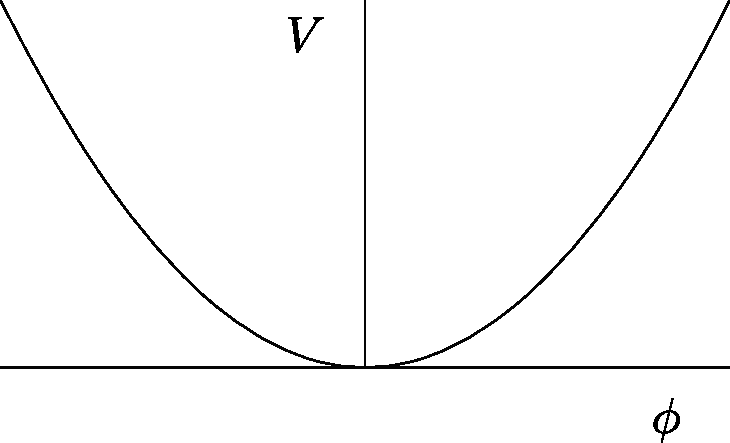
\includegraphics[scale=0.8]{vphi2}
  \caption{$V(\phi)=\frac{1}{2}\mu^2 \phi^2$ con $\mu^2\gt 0$} %noinstiki
  \label{fig:x2} %noinstiki
\end{figure} %noinstiki <div id="fig:x2">Figura: Un mínimo</div>
%noinstiki![cuerda](http://gfif.udea.edu.co/figfs/vphi2.png)
%noinstiki

Si $\mu^2\lt 0$, no existe un mínimo del potencial alrededor del cual el campo pueda oscilar. Además el alejamiento del campo del punto de simetría del potencial no cuesta energía. Por consiguiente en ese caso, el término de interacción
\begin{equation}
  V(\phi)=\tfrac{1}{2}\mu^2   \qquad 
  \mu^2\lt 0,
\end{equation}
no puede interpretarse como un término de masa en el Lagrangiano dado por la ec.~\eqref{eq:83qft}. 

Consideremos ahora el potencial
\begin{equation}
  V(\phi)=\tfrac{1}{2}\mu^2\phi^2+\tfrac{1}{4}\lambda\phi^4
  \qquad   \mu^2\lt 0,\ \lambda\gt 0
\end{equation}
que mantiene la simetría bajo la transformación discreta $\phi\to-\phi$. $\lambda\gt 0$ garantiza la aparición de los dos mínimos que se muestran el la figura \ref{fig:x2l}. Si la energía es suficientemente alta como se muestra en la figura~\ref{fig:x2l}, las excitaciones son simétricas con respecto al máximo del potencial y el término en $\mu^2$ no puede interpretarse como masa para la partícula escalar. 

%noinstiki
\begin{figure} %noinstiki
  \centering %noinstiki
  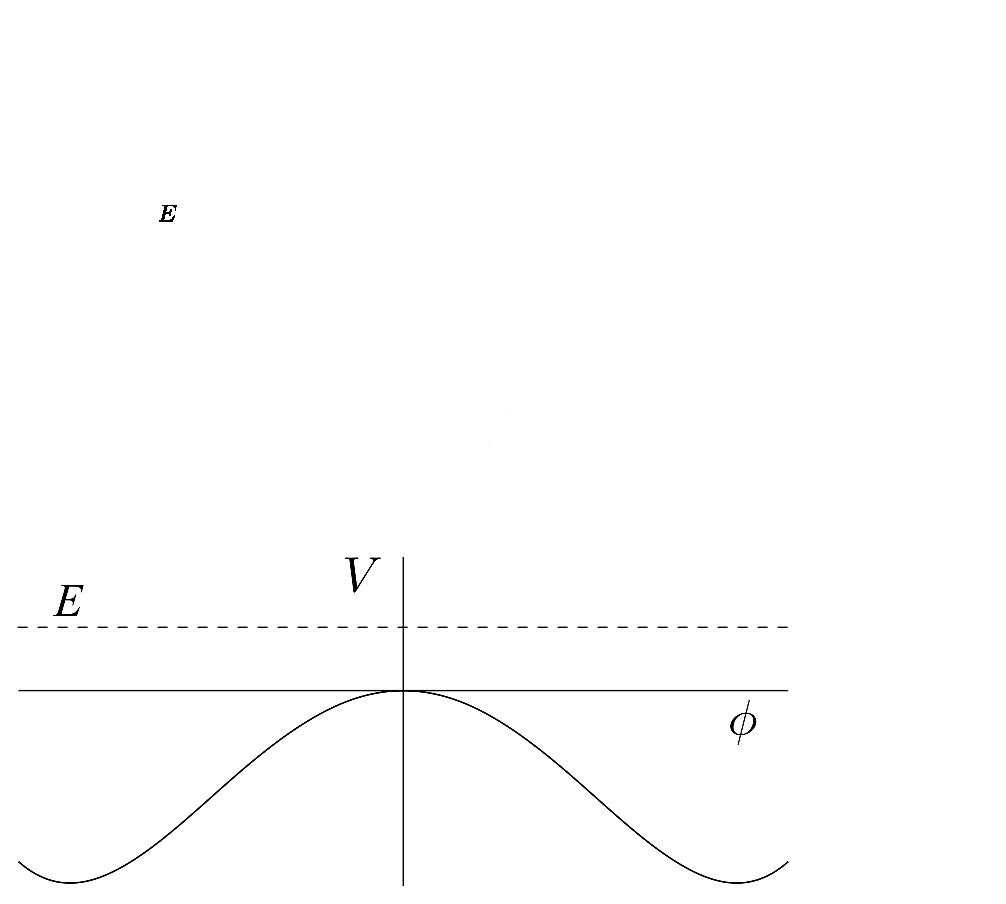
\includegraphics{vphi4}
  \caption{$V(\phi)=\frac{1}{2}\mu^2 \phi^2+\frac{1}{4}\lambda\phi^4$ con $\mu^2\lt 0$, y $\lambda\gt 0$. Simetría exácta} %noinstiki
  \label{fig:x2l} %noinstiki
\end{figure} %noinstiki <div id="fig:x2l">Figura: Mínimos degenerados</div>
%noinstiki![cuerda](http://gfif.udea.edu.co/figfs/vphi4.png)
%noinstiki
Sin embargo, si la energía es suficientemente baja como se muestra en la figura~\ref{fig:x2lm}, las excitaciones alrededor del mínimo dan lugar a la aparición de un término de masa para el campo escalar. Además, dichas excitaciones no respetan la simetrías $\phi\to-\phi$. En tal caso decimos que la simetría ha sido espontáneamente rota: aunque el Lagrangiano mantiene la simetría original, el vacío la rompe. 

%noinstiki
\begin{figure} %noinstiki
  \centering %noinstiki
  %noinstiki
  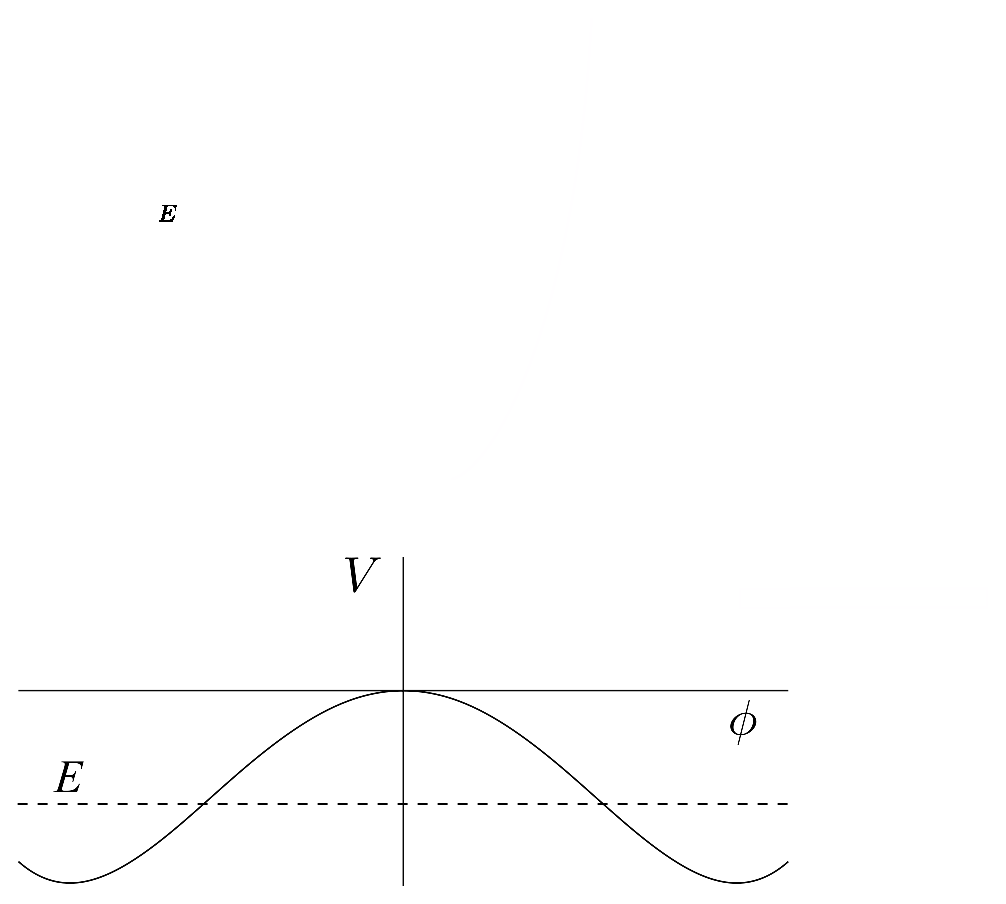
\includegraphics{vphi4m}
  \caption{$V(\phi)=\frac{1}{2}\mu^2 \phi^2+\frac{1}{4}\lambda\phi^4$ con $\mu^2\lt 0$, y $\lambda\gt 0$. Simetría espontáneamente rota.} %noinstiki
  \label{fig:x2lm} %noinstiki
\end{figure}  %noinstiki <div id="fig:x2lm">Figura: Simetría espontáneamente rota  </div>
%noinstiki![vphi4lm](http://gfif.udea.edu.co/figfs/vphi4lm.png)
%noinstiki

Para analizar cuantitativamente el espectro de partículas es necesario expandir el campo alrededor del mínimo y determinar las excitaciones. Establezcamos en primer lugar los mínimos del potencial. La $\partial V/\partial\phi=0$ da lugar a
\begin{align}
  \mu^2\phi+\lambda\phi^3&=0\\
  \phi(\mu^2+\lambda\phi^2)&=0,
\end{align}
con extremos $\phi_{\text{max}}=0$, y 
\begin{equation}
  \label{eq:90qft}
  \phi_{\text{min}}\equiv\langle\phi\rangle\equiv v=\pmm\sqrt{\frac{-\mu^2}{\lambda}}.
\end{equation}
De hecho 
\begin{equation}
  \frac{\partial^2V}{\partial\phi^2}=\mu^2+3\lambda\phi^2.
\end{equation}
$\phi=0$ corresponde a un máximo, mientras que la segunda derivada para $\phi=\pmm\sqrt{-\mu^2/\lambda}$ es $-2\mu^2\gt 0$ y corresponden a los mínimos. Expandiendo el campo alrededor del mínimo
\begin{equation}
  \phi(x)=H(x)+v
\end{equation}
\begin{align}
  V(\phi)=&\tfrac{1}{2}\mu^2 \phi^2+\tfrac{1}{4}\lambda\phi^4\nonumber\\
  =&\tfrac{1}{2}\mu^2 (H+v)^2+\tfrac{1}{4}\lambda(H+v)^4\nonumber\\
  =&\tfrac{1}{2}\mu^2 (H+v)^2+\tfrac{1}{4}\lambda(H+v)^4\nonumber\\
  =&\tfrac{1}{2}\mu^2 \left(H^2+2vH+v^2\right)+\tfrac{1}{4}\lambda\left(H^2+2vH+v^2\right)^2\nonumber\\
  =&\tfrac{1}{2}\mu^2 \left(H^2+2vH+v^2\right)+\tfrac{1}{4}\lambda\left[H^4+2H^2\left(2vH+v^2\right)+\left(2vH+v^2\right)^2\right]\nonumber\\
  =&\tfrac{1}{2}\mu^2 \left(H^2+2vH+v^2\right)+\tfrac{1}{4}\lambda\left[H^4+4vH^3+2H^2v^2+4v^2H^2+4v^3H+v^4\right]\nonumber\\
  =&\tfrac{1}{2}\mu^2 \left(H^2+2vH+v^2\right)+\tfrac{1}{4}\lambda\left[H^4+4vH^3+6H^2v^2+4v^3H+v^4\right]\nonumber\\
  =&\tfrac{1}{2}\mu^2H^2-\tfrac{3}{2}H^2\mu^2+\mu^2vH-\mu^2vH+\tfrac{1}{2}\mu^2v^2-\tfrac{1}{4}\mu^2v^2+\tfrac{1}{4}\lambda\left[H^4+4vH^3\right]\nonumber\\
\label{eq:84qft}
V(H)=&\tfrac{1}{2}\left(-2\mu^2\right)H^2+\lambda vH^3+\tfrac{1}{4}\lambda H^4+\tfrac{1}{4}\mu^2v^2,
\end{align}
y
\begin{equation}
  \label{eq:88qft}
  \mathcal{L}_H=\tfrac{1}{2}\partial^\mu H\partial_\mu H-\tfrac{1}{2}\left(-2\mu^2\right)H^2-\lambda vH^3-\tfrac{1}{4}\lambda H^4+\text{constant}.
\end{equation}
Entonces $H$ adquiere una masa $-2\mu^2$ y no es invariante bajo $H\to-H$. 

Otro método es usar las ecuaciones de mínimo $-\mu^2=\lambda v^2$, para eliminar un parámetro del potencial:
\begin{align}
  V(\phi)&=-\tfrac{1}{2}\lambda v^2\phi^2+\tfrac{1}{4}\lambda\phi^4\nonumber\\
  =&-\tfrac{1}{2}\lambda v^2 \left(H^2+2vH+v^2\right)+\tfrac{1}{4}\lambda\left[H^4+4vH^3+6H^2v^2+4v^3H+v^4\right]\nonumber\\
  =&\lambda v^2H^2+\lambda vH^3+\tfrac{1}{4}\lambda H^4+\text{constant}.
\end{align}
Podemos escribir el potencial en términos del  nuevo campo como
\begin{align}
\label{eq:higgspot}
  V(H)=\frac{1}{2}m_H^2H^2+\frac{1}{2}\frac{m_H^2}{v}H^3+\frac{1}{8}\frac{m_H^2}{v^2} H^4\,.
\end{align}
donde
\begin{equation}
\label{eq:higgsmass}
  m_H^2=2\left|\mu^2\right|=2\lambda v^2
\end{equation}

Consideremos ahora un campo escalar complejo sin término de masa, pero con potencial:
\begin{equation}
  \label{eq:85qft}
  \mathcal{L}=\partial^\mu\phi^*\partial_\mu\phi-V(\phi)
\end{equation}
\begin{equation}
  V(\phi)=\mu^2\phi^*\phi+\lambda(\phi^*\phi)^2 
  \qquad 
  \mu^2\lt 0,\ \lambda\gt 0 
\end{equation}
La simetría del Lagrangiano corresponde a $U(1)$ global. Este potencial corresponde al ``sombrero mexicano'', como se ilustra en la Figura \ref{fig:mexicanhat}. Para una energía suficientemente baja de manera que el campo deba oscilar alrededor del mínimo aparecen dos tipos de excitaciones. Una sobre las paredes  que cuestan energía y corresponden a un campo escalar masivo como en el caso anterior, y otra a lo largo de la circunferencia de mínimo, que corresponde a una partícula escalar sin masa, y es llamada bosón del Golstone. 



\begin{figure}
  \centering
  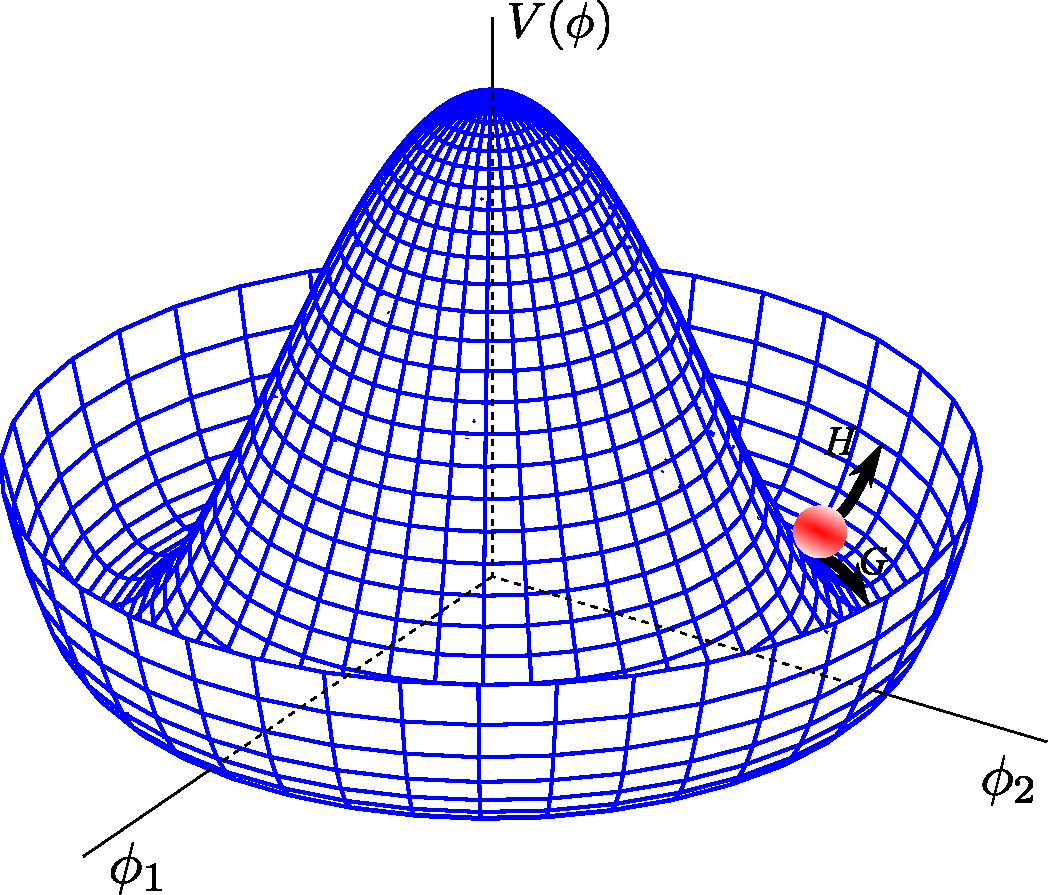
\includegraphics[scale=0.5]{mexicanhat}
  \caption{Potential for complex scalar field}
  \label{fig:mexicanhat}
\end{figure}



El Lagrangiano escalar complejo es equivalente al Lagragiano de dos campos escalares reales con los mismos paramétros. Para un conjunto de $N$ campos reales tenedremos (suma sobre $i$) \cite{Peskin}\footnote{§ 11.1}: 
\begin{align}
  \mathcal{L}=\frac{1}{2}\partial_\mu\phi^i\partial_\mu\phi_i-\frac{1}{2}\mu^2\phi_i\phi^i-\frac{1}{2}\mu^2\left(\phi_i\phi^i\right)^2\,,
\end{align}
que es invariante bajo una simetría $O(N)$
\begin{align}
  \phi^i\to{\phi'}^i=R^{ij}\phi^j\,,
\end{align}
para cualquier matriz $N\timesm  N$ ortogonal $R$. El análisis para $N=2$ da lugar a un bosón de Goldstone. El anális para $N>2$ es el mismo y por cada campo real que se introduzca aparece un nuevo bosón de Goldstone \cite{Peskin}:
\begin{quote}
  [\ldots] there are not continuous symmetries for $N=1$, while for $N=2$ there is a single direction of rotation. A rotation in $N$ dimensions can be in any one of $N(N-1)$ planes, so the $O(N)$--symmetric theory has $N(N-1)/2$ continuous symmetries. After spontaneous symmetry breaking there are $(N-1)(N-2)/2$  remaining symmetries corresponding to rotations of the $(N-1)$ [non massive] fields. The number of \emph{broken} symmetries is the difference, $N-1$.
\end{quote}
Entonces tenemos el siguiente teorema \cite{Peskin}
\begin{quote}
\emph{Goldstone's theorem states that for every spontaneously broken continuous symmetry, the theory must contain a massless particle.}
\end{quote}

Also from \cite{Peskin}\footnote{Introduction to Chapter 20}
\begin{quote}
  In a global symmetry  that is spontaneously broken the symmetry currents are still conserved and interactions are similarly restricted [the Lagrangian keeps the symmetry], but the vacuum state does not respect the symmetry and the particles do not form obvious symmetry multiplets. Instead, such a theory contains massless particles, Goldstone bosons, one for each generator of the spontaneously broken symmetry. The third case is that of a local, or gauge, symmetry. [\ldots] such a symmetry requires the existence of a massless vector field for each symmetry generator, and the interactions among these fields are highly restricted.

It is now only natural to consider a fourth possibility: What happens if we include both local gauge invariance  and spontaneous symmetry breaking in the same theory?
\end{quote}
 

En el caso de la Acción invariante gauge local bajo el Grupo $U(1)$, tenemos el Lagrangiano \eqref{eq:56qft}:
\begin{equation}
  \label{eq:89qft}
  \mathcal{L}=\left(\mathcal{D}^\mu\phi\right)^*\mathcal{D}_\mu\phi-\mu^2\phi^*\phi-\lambda\left(\phi^*\phi\right)^2-\tfrac{1}{4}F^{\mu\nu}F_{\mu\nu}
  \qquad 
  \mu^2\lt 0\text{ and } \lambda\gt 0
\end{equation}
Para obtener directamente el espectro después de la ruptura espontánea de simetría es conveniente usar la transformación gauge de la ec.~\eqref{eq:86qft}. Haciendo $\theta(x)=-\eta(x)$:
\begin{equation}
\label{eq:87qft}
   \phi\to\phi'=e^{i\theta(x)}e^{i\eta(x)}\left(\frac{H(x)+v}{\sqrt{2}}\right)=\frac{H(x)+v}{\sqrt{2}}
\end{equation}
\begin{align}
  \mathcal{L}\to\mathcal{L}' &=\left[\left(\mathcal{D}^\mu\right)'\phi'\right]^*\left(\mathcal{D}_\mu\right)'\phi'-\mu^2\left(\phi^*\right)'\phi'-\lambda\left[\left(\phi^*\right)'\phi'\right]^2-\tfrac{1}{4}\left(F^{\mu\nu}F_{\mu\nu}\right)'\nonumber\\
 &=\tfrac{1}{2}\left[\partial^\mu H+ig{A'}^\mu(H+v)\right]\left[\partial_\mu H-ig{A'}_\mu(H+v)\right]-\tfrac{1}{2}\mu^2(H+v)^2-\tfrac{1}{4}\lambda(H+v)^4-\tfrac{1}{4}F^{\mu\nu}F_{\mu\nu}
\end{align}
En adelante omitiremos las primas, aunque debe estar claro que se esta trabajando en el gauge específico de la ec.~\eqref{eq:87qft}. Entonces
\begin{align}
  \mathcal{L}&=\tfrac{1}{2}\partial^\mu H\partial_\mu H-\tfrac{1}{2}\mu^2(H+v)^2-
  \tfrac{1}{4}\lambda(H+v)^4+\tfrac{1}{2}g^2A^\mu A_\mu(H+v)^2
  -\tfrac{1}{4}F^{\mu\nu}F_{\mu\nu}.
\end{align}
Usando la ec.~\eqref{eq:84qft}
\begin{equation}
  \label{eq:94qft}
  \mathcal{L}=\mathcal{L}_H+\mathcal{L}_{A^\mu}+\tfrac{1}{2}g^2A^\mu A_\mu H^2+g^2vA^\mu A_\mu H,
\end{equation}
donde $\mathcal{L}_H$ esta dado por la ec.~\eqref{eq:88qft} y
\begin{equation}
  \mathcal{L}_{A^\mu}=-\tfrac{1}{4}F^{\mu\nu}F_{\mu\nu}+\tfrac{1}{2}g^2v^2A^\mu A_\mu.
\end{equation}
Teniendo en cuenta la ec.~\eqref{eq:23qft} para el Lagrangiano de Proca, vemos que como consecuencia de la ruptura espontánea de simetría el campo gauge ha adquirido una masa
\begin{equation}
  m_{A^\mu}=gv.
\end{equation}

El mecanismo completo mediante el cual, a partir de un Lagrangiano invariante gauge local, los bosones gauge adquieren masa se llama \emph{mecanismo de Higgs} \cite{Higgs:1964pj}. La partícula escalar que adquiere masa se llama Higgs, mientras que el bosón de Goldstone es absorbido por campo gauge como modo longitudinal. 

El número de grados de libertad independientes en el Lagrangiano original en la ec.~\eqref{eq:89qft} es cuatro. Correspondientes a los dos grados de libertad del bosón gauge no masivo y los dos del campo escalar complejo. En el Lagrangiano final en la ec.~\eqref{eq:94qft} no aparece el bosón de Goldstone. Sin embargo esto no es un problema porque dicho Lagrangiano también tiene cuatro grados de libertad correspondientes a  los tres grados de libertad del bosón gauge masivo y al grado de libertad del bosón de Higgs. 

\end{frame}


\section{Fermiones quirales de cuatro componentes}
\label{sec:ferm-quir-de}

Sea
\begin{align}
  P_L\equiv&\frac{1-\gamma_5}{2}\nonumber\\
  P_R\equiv&\frac{1+\gamma_5}{2}\,.
\end{align}
Además
\begin{align}
  \psi_L\equiv P_L\psi\nonumber\\
  \psi_R\equiv P_R\psi\,.
\end{align}
Entonces
\begin{align}
  \psi=\psi_L+\psi_R\,.
\end{align}

Las matrices $P_{L,R}$ tienen las propiedades
\begin{align}
  P_L+P_R&=1 & P_{L,R}^2&=P_{L,R}P_{L,R}=P_{L,R}\nonumber\\
  P_L P_R&=0& P_{L,R}^\dagger&=P_{L,R}\,.
\end{align}
Usando la ec.~(\ref{eq:218qft})
\begin{align}
  P_{L,R}\gamma^\mu=\frac{1\mp\gamma_5}{2}\gamma^\mu=\gamma^\mu\frac{1\pmm\gamma_5}{2}=\gamma^\mu P_{R,L}
\end{align}
Para escribir el Lagrangiano en término de los nuevos $\psi_{L,R}$ debemos tener en cuenta que
\begin{align}
  \overline{\psi_{L,R}}=(P_{L,R}\psi)^\dagger\gamma^0=\psi^\dagger P_{L,R}\gamma^0=\psi^\dagger\gamma^0P_{R,L}=\overline{\psi}P_{R,L}
\end{align}
\begin{align}
  \label{eq:221qft}
  \mathcal{L}=&i\overline{\psi}\gamma^\mu\partial_\mu\psi-m\overline{\psi}\psi\nonumber\\
  =&i\overline{\psi}(P_L+P_R)\gamma^\mu\partial_\mu\psi-m\overline{\psi}(P_L+P_R)\psi\nonumber\\
  =&i\overline{\psi}P_L\gamma^\mu\partial_\mu\psi+i\overline{\psi}P_R\gamma^\mu\partial_\mu\psi-m\overline{\psi}P_L\psi-m\overline{\psi}P_R\psi\nonumber\\
  =&i\overline{\psi}P_L P_L\gamma^\mu\partial_\mu\psi+i\overline{\psi}P_R P_R\gamma^\mu\partial_\mu\psi-m\overline{\psi}P_L P_L\psi-m\overline{\psi}P_R P_R\psi\nonumber\\
  =&i\overline{\psi}P_L\gamma^\mu\partial_\mu P_R\psi+i\overline{\psi}P_R\gamma^\mu\partial_\mu P_L\psi-m\overline{\psi}P_L P_L\psi-m\overline{\psi}P_R P_R\psi\nonumber\\
  =&i\overline{\psi_R}\gamma^\mu\partial_\mu\psi_R+i\overline{\psi_L}\gamma^\mu\partial_\mu\psi_L-m(\overline{\psi_R}\psi_L+\overline{\psi_L}\psi_R)\,.
\end{align}
En términos de espinores de izquierdos y derechos de cuatro componentes la transformación de paridad 
\begin{align}
  \label{eq:220qft}
  t&\to t&\mathbf{x}&\to -\mathbf{x}&\psi_L(t,\mathbf{x})\to&\psi_R(t,-\mathbf{x}),& \psi_R(t,\mathbf{x})&\to\psi_L(t,-\mathbf{x})\nonumber\\
  \partial_0&\to \partial_0&\boldsymbol{\nabla}&\to -\boldsymbol{\nabla}&\psi_L(t,\mathbf{x})\to&\psi_R(t,-\mathbf{x}),& \psi_R(t,\mathbf{x})&\to\psi_L(t,-\mathbf{x})\,.
\end{align}
Además $\mathbf{L}=\mathbf{r}\timesm \mathbf{p}\to(-\mathbf{r})\timesm (-\mathbf{p})=\mathbf{L}$, y como $\gamma^\mu$ esta asociado al momento angular intrínsico, entonces también $\gamma^\mu\to\gamma^\mu$


Entonces la transformación de paridad da lugar a (sin tener en cuenta el cambio de argumento en los campos que desaparece en la integral de la Acción) y la representación de paridad \eqref{eq:parityrep}:
\begin{align}
  \overline{\psi_R}\gamma^\mu\partial_\mu\psi_R=\overline{\psi_R}\gamma^0\partial_0\psi_R+\overline{\psi_R}\boldsymbol{\gamma}\cdot\boldsymbol{\nabla}\psi_R 
\to&\overline{\psi_L}\gamma^0\partial_0\psi_L-\overline{\psi_L}\boldsymbol{\gamma}\cdot\boldsymbol{\nabla}\psi_L\nonumber\\
=&\overline{\psi_L}\gamma^0\partial_0\psi_L+\overline{\psi_L}\boldsymbol{\gamma}^\dagger\cdot\boldsymbol{\nabla}\psi_L\nonumber\\
=&\overline{\psi_L}\gamma^0\gamma^0\gamma^0\partial_0\psi_L+\overline{\psi_L}\gamma^0\boldsymbol{\gamma}\gamma^0\cdot\boldsymbol{\nabla}\psi_L\nonumber\\
=&\overline{\psi_L}\tilde\gamma^0\partial_0\psi_L+\overline{\psi_L}\tilde{\boldsymbol{\gamma}}\cdot\boldsymbol{\nabla}\psi_L\nonumber\\
=&\overline{\psi_R}\tilde\gamma^\mu\partial_\mu\psi_R\,.
\end{align}
Entonces
\begin{align}
   \mathcal{L}\to\mathcal{L}'=&i\overline{\psi_R}\tilde\gamma^\mu\partial_\mu\psi_R+i\overline{\psi_L}\tilde\gamma^\mu\partial_\mu\psi_L-m(\overline{\psi_R}\psi_L+\overline{\psi_L}\psi_R)\,,
\end{align}
donde $\tilde\gamma^\mu=U\gamma^\mu U^\dagger$, con $U=\gamma^0$. Como las dos representaciones dan lugar a la misma física, podemos decir que la Acción en términos de espinores $L,R$ de cuatro componentes es invariante bajo la transformación de paridad.

La existencia de ambos espinores $\psi_{L,R}$ garantizan que el Lagrangiano de Dirac es invariante bajo la transformación de paridad. 

La corriente de la electrodinámica cuántica en ec.~\eqref{eq:222qft} (o la de la cromodinámica cuántica, ec.~\eqref{eq:223qft}) conservan paridad ya que, siguiendo los mismos pasos que en la ec.~\eqref{eq:221qft}
\begin{align}
  \label{eq:224qft}
  \overline{\psi}\gamma^\mu\psi=\overline{\psi_L}\gamma^\mu\psi_L+\overline{\psi_R}\gamma^\mu\psi_R\to\overline{\psi_L}\gamma^\mu\psi_L+\overline{\psi_R}\gamma^\mu\psi_R\,.
\end{align}
Si para alguna partícula, como es el caso del neutrino, no existe la componente derecha, entonces la correspondiente interacción vectorial viola paridad y no puede tener interacciones electromagnéticas ni fuertes, es decir, no se acopla con el ftón o los gluones. Además dicha partícula no puede tener masa de Dirac. En el caso del neutrino esto se entiende pues al no tenr carga eléctrica sólo reuiere dos grados de libertad independientes.

De otro lado, si una determinada interacción, como es el caso de la interacción débil, solo participa la componente izquierda de la ec.~\eqref{eq:224qft}, está corresponde a una interacción del tipo
\begin{align}
  \overline{\psi}_L\gamma^\mu\psi_L&=\overline{\psi}P_R\gamma^\mu P_L\psi=\overline{\psi}\gamma^\mu P_L\psi\nonumber\\
  &=\overline{\psi}\gamma^\mu\left(\frac{1-\gamma_5}{2}\right)\psi\nonumber\\
  &=\tfrac{1}{2}\overline{\psi}\left(\gamma^\mu-\gamma^\mu\gamma_5\right)\psi\,,
\end{align}
que de acuerdo a la asignación en la Tabla corresponde a una corriente V--A. 

\section{Standard model Lagrangian}
\label{sec:stand-model-lagr}

\begin{frame}[fragile,allowframebreaks]
The known matter is build from the elementary set of particles defined in table
\begin{table}
  \centering
  \begin{tabular}{l|l|c|r}
    Type &Name & Symbol&Charge\\\hline{}
   leptons& electron & $e$& $-1$\\
          & neutrino & $\nu$ & $0$\\\hline{}
   quarks &up quark & $u_1,u_2,u_3$ & $2/3$\\
          &down quark & $d_1,d_2,d_3$& $-1/3$\\
  \end{tabular}
  \caption{Elementary fermions. The symbol represent both the particle, e.g $e^-$, as the antiparticle, e.g, $e^+$. The lectric chage is given in units of the electron chage $e$  }
  \label{tab:ef}
\end{table}

we further define the color triplets of quarks as
\begin{align}
  u=&
  \begin{pmatrix}
    u_1 \\ u_2\\ u_3\\
  \end{pmatrix}
  &d=&
  \begin{pmatrix}
    d_1 \\ d_2 \\ d_3\\
  \end{pmatrix}
\end{align}


The free Lagrangian containing this particles can be written as
\begin{align}
  \mathcal{L}_{\text{free}}=&i\overline{e}\gamma^\mu\partial_\mu e-m_e\overline{e}e+i\overline{\nu}\gamma^\mu\partial_\mu\nu
+i\overline{u}\gamma^\mu\partial_\mu u-m_u\overline{u}u+i\overline{d}\gamma^\mu\partial_\mu d-m_d\overline{d}d\nonumber\\
=&i\overline{e_L}\gamma^\mu\partial_\mu e_L+i\overline{e_R}\gamma^\mu\partial_\mu e_R-m_e(\overline{e_R}e_L+\overline{e_L}e_R)+i\overline{\nu_L}\gamma^\mu\partial_\mu\nu_L\nonumber\\
&+i\overline{\nu_R}\gamma^\mu\partial_\mu\nu_R+i\overline{u_L}\gamma^\mu\partial_\mu u_L+i\overline{u_R}\gamma^\mu\partial_\mu u_R\nonumber\\
&-m_e(\overline{u_R}u_L+\overline{u_L}u_R)
i\overline{d_L}\gamma^\mu\partial_\mu d_L+i\overline{d_R}\gamma^\mu\partial_\mu d_R-m_e(\overline{d_R}d_L+\overline{d_L}d_R)\,.
\end{align}
donde,
\begin{align}
  \nu_{L,R}=&P_{L,R}\nu,& e_{L,R}=&P_{L,R}\,e\nonumber\\
  u_{L,R}=&P_{L,R}\,u,& d_{L,R}=&P_{L,R}\,d\,.
\end{align}

\subsection*{Corrientes V--A}
\label{sec:corrientes-v}
En las interacciones débiles sólo participan las partes izquierdas de los campos. Esto nos permite prescindir del $\nu_R$, pues no tiene carga eléctrica, fuerte, o débil
\begin{align}
  \mathcal{L}_{\text{free}}
=&i\overline{e_L}\gamma^\mu\partial_\mu e_L+i\overline{e_R}\gamma^\mu\partial_\mu e_R-m_e(\overline{e_R}e_L+\overline{e_L}e_R)+
i\overline{\nu_L}\gamma^\mu\partial_\mu\nu_L\nonumber\\
&+i\overline{u_L}\gamma^\mu\partial_\mu u_L+i\overline{u_R}\gamma^\mu\partial_\mu u_R\nonumber\\
&-m_e(\overline{u_R}u_L+\overline{u_L}u_R)
i\overline{d_L}\gamma^\mu\partial_\mu d_L+i\overline{d_R}\gamma^\mu\partial_\mu d_R-m_e(\overline{d_R}d_L+\overline{d_L}d_R)\,.
\end{align}


\subsection*{Simetría global $SU(3)_c\timesm  SU(2)_L\timesm  U(1)_Y$}
\label{sec:simetr-glob-su2_l}

En el contexto de las interacciones débiles un $e_L$ es completamente equivalente a un campo $\nu_L$. Es decir, el Lagrangiano debe ser invariante bajo una transformación $SU(2)_L$ de esos campos. La diferencia entre ellos son sus respectivas cargas electricas y sus masas. Asumiendo que ambos campos tienen una misma hipercarga, asociada a una nueva simetría Abeliana $U(1)_Y$, podríamos esperar que la corriente electromagnética apropiada pueda obtenerse a partir del Grupo semisimple $SU(2)_L\timesm  U(1)_Y$. Además las respectivas masas se podrían obtener a partir del mecanismo de Higgs. 

La simetría $SU(2)_L$ entre las partes izquierdas del neutrino y el electrón, y entre las partes izquierdas de los quarks up y down, se establece  definiendo los dobletes:
  \begin{align}
    L\equiv\begin{pmatrix}
      \nu_L\\
      e_L      
    \end{pmatrix}\qquad   Q=&\begin{pmatrix}
    u_L\\
    d_L
  \end{pmatrix}\,,
  \end{align}
De otro lado, La invarianza bajo $U(1)_Y$ requiere que
\begin{align}
  Y_L=&Y_{\nu_L}=Y_{e_L}\nonumber\\
  Y_Q=&Y_{u_L}=Y_{d_L}\,.
\end{align}
El generador de carga eléctrica $\widehat{Q}$, se va obtener a partir de una combinación lineal del generador diagonal de $SU(2)_L$, $T_3$, y del generador de hipercarga, $Y$.

Bajo la simetría $SU(2)_L$, los campos transforman como:
 \begin{align}
  L\to L'=&\exp(i T^i \theta_i)L\approx(1+i T^i\theta_i)L\nonumber\\
  Q\to Q'=&\exp(i T^i \theta_i)Q\approx(1+i T^i\theta_i)Q\nonumber\\
  e_R\to& e'_R=e_R\nonumber\\
  u_R\to& u'_R=u_R\nonumber\\
  d_R\to& d'_R=d_R\,.
\end{align}
donde
\begin{align}
  T^i=\frac{\tau^i}{2}\,,
\end{align}
y $\tau^i$ son las matrices de Pauli dadas en la ec.~\eqref{eq:paulimatr}.

Claramente el término de masa $m_e$ en la ec.~(\ref{eq:261qft}) no es invariante bajo la simetría $SU(2)_L$. El Lagrangiano en la ec.~(\ref{eq:261qft}), sin término de masa, puede reescribirse de manera que exhíba de forma más explicita la invarianza bajo $SU(2)_L$ como
\begin{align}
  \mathcal{L}_{\text{free}}
=&i\overline{e_L}\gamma^\mu\partial_\mu e_L+i\overline{e_R}\gamma^\mu\partial_\mu e_R+i\overline{\nu_L}\gamma^\mu\partial_\mu\nu_L\nonumber\\
&+i\overline{u_L}\gamma^\mu\partial_\mu u_L+i\overline{u_R}\gamma^\mu\partial_\mu u_R
+i\overline{d_L}\gamma^\mu\partial_\mu d_L+i\overline{d_R}\gamma^\mu\partial_\mu d_R\nonumber\\
=&i\overline{L}\gamma^\mu\partial_\mu L+i\overline{Q}\gamma^\mu\partial_\mu Q+i\overline{e_R}\gamma^\mu\partial_\mu e_R
+i\overline{u_R}\gamma^\mu\partial_\mu u_R
+i\overline{d_R}\gamma^\mu\partial_\mu d_R\,.
\end{align}


\subsection*{Simetría gauge local $SU(3)_c\timesm  SU(2)_L\timesm  U(1)_Y$}

Para obtener la interacciones del modelo estándar, reemplazamos las derivadas normales por derivadas covariantes.

Proponemos entonces el Lagrangiano
\begin{align}
     \mathcal{L}=&i\overline{Q}\gamma^\mu\mathcal{D}_\mu Q+i\overline{L}\gamma^\mu\mathcal{D}_\mu L+
i\overline{e_R}\gamma^\mu\mathcal{D}_\mu {e_R}+i\overline{d_R}\gamma^\mu\mathcal{D}_\mu {d_R}+i\overline{u_R}\gamma^\mu\mathcal{D}_\mu {u_R}
\nonumber\\
     &-\tfrac{1}{4}G^{\mu\nu}_a G_{\mu\nu}^a-\tfrac{1}{4}W^{\mu\nu}_i W_{\mu\nu}^i-\tfrac{1}{4}B^{\mu\nu} B_{\mu\nu}\,,
\end{align}
Donde
\begin{align}
  \mathcal{D}^\mu&\equiv\partial^\mu-i g_s\frac{\lambda^a}{2}G^\mu_a-i g \frac{\tau^i}{2}W^\mu_i-i g'YB^\mu\,.
\end{align}
donde
\begin{align*}
  \Lambda^a\equiv\frac{\lambda^a}{2},\ a=1,2,\ldots,8 &\qquad\text{8 generadores de $SU(3)_c$}\\
  T^i\equiv\frac{\tau^i}{2},\ i=1,2,3 &\qquad\text{3 generadores de $SU(2)_L$}\\
  Y &\qquad\text{generador de $U(1)_Y$}
\end{align*}

All the particles in this Lagrangian are massless. It is only good for the gluons and the Abelian gauge boson, but is no realist for the fermions of the weak gauge bosons $W_\mu^i$. To solve this problem, we postulate a new complex scalar doublet with four degree of freedom:
\begin{equation}
  \Phi=
  \begin{pmatrix}
    \phi^+\\
    \phi^0
  \end{pmatrix}\,.
\end{equation} 
The full Lagrangian involving those fields are 
\begin{align}
     \mathcal{L}=&i\overline{Q}\gamma^\mu\mathcal{D}_\mu Q+i\overline{L}\gamma^\mu\mathcal{D}_\mu L+
i\overline{e_R}\gamma^\mu\mathcal{D}_\mu {e_R}+i\overline{d_R}\gamma^\mu\mathcal{D}_\mu {d_R}+i\overline{u_R}\gamma^\mu\mathcal{D}_\mu {u_R}
\nonumber\\
     &-\tfrac{1}{4}G^{\mu\nu}_a G_{\mu\nu}^a-\tfrac{1}{4}W^{\mu\nu}_i W_{\mu\nu}^i-\tfrac{1}{4}B^{\mu\nu} B_{\mu\nu}\nonumber\\
     &+(\mathcal{D}_\mu\Phi)^\dagger\mathcal{D}^\mu\Phi-\mu^2\Phi^\dagger\Phi-\lambda(\Phi^\dagger\Phi)^2\nonumber\\
     &-(h_e\overline{L}\Phi e_R+h_d\overline{Q}\Phi d_R+h_u\overline{Q}\widetilde{\Phi}u_R+\text{h.c})\nonumber\\
     =&\mathcal{L}_{\text{fermion}}+\mathcal{L}_{\text{gauge}}
     +\mathcal{L}_{WBH}
     -\mathcal{L}_{\text{Yukawa}}\,.
\end{align}
donde $\mu^2<0$, y $\lambda>0$,
\begin{align}
  \widetilde{\Phi}=i\tau_2\Phi^*\,,
\end{align}
\begin{align}
  \label{eq:smscalar}
\mathcal{L}_{\text{fermion}}=&i\overline{Q}\gamma^\mu\mathcal{D}_\mu Q+i\overline{L}\gamma^\mu\mathcal{D}_\mu L+
i\overline{e_R}\gamma^\mu\mathcal{D}_\mu {e_R}+i\overline{d_R}\gamma^\mu\mathcal{D}_\mu {d_R}+i\overline{u_R}\gamma^\mu\mathcal{D}_\mu {u_R}\nonumber\\
\mathcal{L}_{\text{gauge}}=& -\tfrac{1}{4}G^{\mu\nu}_a G_{\mu\nu}^a-\tfrac{1}{4}W^{\mu\nu}_i W_{\mu\nu}^i-\tfrac{1}{4}B^{\mu\nu} B_{\mu\nu}\nonumber\\
  \mathcal{L}_{WBH}=&(\mathcal{D}_\mu\Phi)^\dagger\mathcal{D}^\mu\Phi-\mu^2\Phi^\dagger\Phi-\lambda(\Phi^\dagger\Phi)^2\nonumber\\
\mathcal{L}_{\text{Yukawa}}=&h_e\overline{L}\Phi e_R+h_d\overline{Q}\Phi d_R+h_u\overline{Q}\widetilde{\Phi}u_R+\text{h.c}
\end{align}


Bajo una transformación gauge local las derivadas covariantes de los campos (y por consiguiente los campos) transforman como:
\begin{align}
  \mathcal{D}_\mu L&\to\left(\mathcal{D}_\mu L\right)'=\exp\left(-i\theta_iT^i-i\beta Y_L\right)\mathcal{D}_\mu L\nonumber\\
  \mathcal{D}_\mu Q&\to\left(\mathcal{D}_\mu Q\right)'=\exp\left(-i\alpha_a\Lambda^a-i\theta_iT^i-i\beta Y_Q\right)\mathcal{D}_\mu Q\nonumber\\
  \mathcal{D}_\mu \Phi&\to\left(\mathcal{D}_\mu \Phi\right)'=\exp\left(-i\theta_iT^i-i\beta Y_\Phi\right)\mathcal{D}_\mu \Phi\nonumber\\
  \mathcal{D}_\mu e_R&\to\left(\mathcal{D}_\mu e_R\right)'=\exp\left(-i\beta Y_{e_R}\right)\mathcal{D}_\mu e_R=\exp\left(-i\beta Q_{e_R}\right)\mathcal{D}_\mu e_R\nonumber\\
  \mathcal{D}_\mu d_R&\to\left(\mathcal{D}_\mu d_R\right)'=\exp\left(-i\alpha_a\Lambda^a-i\beta Y_{d_R}\right)\mathcal{D}_\mu d_R=\exp\left(-i\alpha_a\Lambda^a-i\beta Q_{d_R}\right)\mathcal{D}_\mu d_R\nonumber\\
  \mathcal{D}_\mu u_R&\to\left(\mathcal{D}_\mu u_R\right)'=\exp\left(-i\alpha_a\Lambda^a-i\beta Y_{u_R}\right)\mathcal{D}_\mu u_R=\exp\left(-i\alpha_a\Lambda^a-i\beta Q_{u_R}\right)\mathcal{D}_\mu u_R\,.
\end{align}
donde $Q_{e_R}=-1$, etc, son las cargas eléctricas asociadas a los campos.

Para los campos del Lagrangiano, debemos asegurarnos de que todos los términos invariantes gauge locales y renormalizables sean considerados. De hecho un término de interacción entre fermiones y el campo escalar, correspondiente a una interacción de Yukawa: $\overline{L}\Phi e_R$ y $\overline{Q}\Phi d_R$ son invariantes bajo transformaciones $SU(3)_c\timesm  SU(2)_L\timesm  U(1)_Y$ si
\begin{align*}
  -Y_L+Y_\Phi+Q_{e_R}=&0\\
  -Y_Q+Y_\Phi+Q_{d_R}=&0\\
  -Y_Q+Y_{\widetilde{\Phi}}+Y_{u_R}=-Y_Q-Y_{\Phi}+Q_{u_R}=&0\,,
\end{align*}
From this set of three equations we obtain the three doublet hypercharges:
\begin{align}
\label{eq:lhyp}
Y_L=-\frac{1}{2}\,,\qquad Y_\Phi=\frac{1}{2}\,,\qquad Y_Q=\frac{1}{6}\,.
\end{align}
En el análisis anterior hemos fijado $Y_{\widetilde{\Phi}}=-Y_\Phi$. Esto es debido a que  si
$\overline{Q}\Phi$ es un invariante $SU(2)_L$, el término ${\tilde \Phi}^\dagger Q$ también es un invariante de $SU(2)$. Explícitamente
\begin{align}
  \widetilde{\Phi}^\dagger Q=&(i\tau_2\Phi^*)^\dagger Q\nonumber\\
  =& \begin{pmatrix}
    {\phi^0}^*\\
    -\phi^-    
  \end{pmatrix}^\dagger Q\nonumber\\
  =&\begin{pmatrix}
    \phi^0 & -\phi^+
  \end{pmatrix}\begin{pmatrix}
    u_L\\
    d_L
  \end{pmatrix}\nonumber\\
  =&\phi^0 u_L - \phi^+ d_L\nonumber\\
  =&\epsilon_{12}Q_1\Phi_2+\epsilon_{21}Q_2\Phi_1\nonumber\\
  =&\epsilon_{ab}Q_a \Phi_b\,.
\end{align}
Bajo una transformación $SU(2)_L$
\begin{align}
\widetilde{\Phi}^\dagger Q\to {\widetilde{\Phi'}}^\dagger Q'=\epsilon_{ab}Q'_a \Phi'_b=&\epsilon_{ab}U_{ac}U_{bd}Q_c \Phi_d\nonumber\\
  =&\epsilon_{cd}\det\mathbf{U} Q_c \Phi_d\nonumber\\
  =&\epsilon_{cd} Q_c \Phi_d\nonumber\\
  =&\widetilde{\Phi}^\dagger Q\,.
\end{align}

Sin perdida de generalidad los cuatro grados de libertad de $\Phi$, pueden escribirse en la forma
\begin{align}
\label{eq:polarhiggs}
  \Phi=&e^{i\eta_j(x)T^j}
  \begin{pmatrix}
    0\\
    \frac{1}{\sqrt{2}}H(x)
  \end{pmatrix}.
\end{align}
El potencial escalar, definido por
\begin{align}
  V(\Phi)=\mu^2\Phi^\dagger\Phi+\lambda(\Phi^\dagger\Phi)^2
\end{align}
se reduce a
\begin{align}
  V(H)=\frac{1}{2}\mu^2H^2+\frac{1}{4}\lambda H^4\,.
\end{align}

\end{frame}
\subsection{Spontaneous symmetry breaking in $SU(3)_c\timesm  SU(2)_L\timesm  U(1)_Y$}

\begin{frame}[fragile,allowframebreaks]
Retornando al doblete de Higgs del modelo estándar en la ec.~\eqref{eq:polarhiggs}, los cuatro grados de libertad de $\Phi$, pueden escribirse en forma polar pero con la parte real neutra desplazada para generar la ruptura espontánea de la simetría $SU(2)_L\timesm  U(1)_Y$
\begin{align}
\label{eq:92qft}
  \Phi=&e^{i\eta_jT^j}
  \begin{pmatrix}
    0\\
    \frac{1}{\sqrt{2}}(H(x)+v)
  \end{pmatrix}\\
  \approx&
  \frac{1}{2}\begin{pmatrix}
    1+i\eta_3&\sqrt{2}i\eta^+\\
    \sqrt{2}i\eta^-&1-i\eta_3
  \end{pmatrix}  \begin{pmatrix}
    0\\
    \frac{1}{\sqrt{2}}(H(x)+v)
  \end{pmatrix}\nonumber\\
  =&\frac{1}{2}\begin{pmatrix}
    i\eta^+H+vi\eta^+\\
    \frac{1}{\sqrt{2}}(H+v-i\eta_3H-i\eta_3 v)
  \end{pmatrix}\nonumber\\
  =&\begin{pmatrix}
    G^+\\
    \frac{1}{\sqrt{2}}(H(x)+v-iG^0)
  \end{pmatrix}.\nonumber
\end{align}
Para $SU(2)_L\timesm  U(1)_Y$ tenemos cuatro generadores y cuatro bosones gauge. De acuerdo a la parametrización en ec.~\eqref{eq:92qft} esperamos que aparezcan tres bosones de Goldstone, de manera que quedará un generador no roto correspondiente a una simetría remanente del vacío $U(1)_Q$
\begin{equation}
  SU(2)\timesm  U(1)_Y\overset{\langle\Phi\rangle}{\longrightarrow}U(1)_Q.
\end{equation}
Se espera entonces que el espectro consista de un bosón de Higgs, tres bosones gauge masivos, y un bosón gauge sin masa.

Para $\alpha=0$, podemos hacer una transformación gauge usando la ec.~\eqref{eq:93qft} sobre el campo $\Phi$, tal que
\begin{equation}
  \label{eq:123qft}
    \Phi\to\Phi'=
  \begin{pmatrix}
    0\\
    \frac{1}{\sqrt{2}}(H(x)+v)
  \end{pmatrix},
\end{equation}
que define el \emph{gauge unitario}. En adelante sin embargo omitiremos las primas sobre los campos transformados $\Phi'$ y $W'_{\mu\nu}$.

Comenzaremos analizando la parte escalar del Lagrangiano del Modelo Estándar para una generación dad en la ec.~\eqref{eq:smscalar}
\begin{equation}
  \mathcal{L}_{WBH}=\frac{1}{2}\left[\mathcal{D}^\mu \begin{pmatrix}
    0\\
    H(x)+v
  \end{pmatrix}\right]^\dagger\mathcal{D}_\mu\begin{pmatrix}
    0\\
    H(x)+v
  \end{pmatrix}-V(H)\,,
\end{equation}
donde $V(H)$ dado en la ec.~\eqref{eq:higgspot}, incluye el término de masa para el bosón de Higgs \eqref{eq:higgsmass}:
\begin{equation}
  m_H^2=2\left|\mu^2\right|=2\lambda v^2
\end{equation}
Como
\begin{align}
      W_\mu=T_i W^{i}_\mu&=
  \frac{1}{2}\begin{pmatrix}
    0&1\\
    1&0
  \end{pmatrix}W^1_\mu+
  \frac{1}{2}\begin{pmatrix}
    0&-i\\
    i&0
  \end{pmatrix}W^2_\mu+
  \frac{1}{2}\begin{pmatrix}
    1&0\\
    0&-1
  \end{pmatrix}W^3_\mu\nonumber\\
  &=
  \frac{1}{2}\begin{pmatrix}
    W^3_\mu                                  &\sqrt{2}\,\dfrac{W^1_\mu-i\,W^2_\mu}{\sqrt{2}}\\
    \sqrt{2}\,\dfrac{W^1_\mu+i\,W^2_\mu}{\sqrt{2}} &-W^3_\mu
  \end{pmatrix}\nonumber\\
  &\equiv
  \frac{1}{2}\begin{pmatrix}
    W^3_\mu&\sqrt{2}W^+_\mu\\
    \sqrt{2}W^-_\mu&-W^3_\mu
  \end{pmatrix}\nonumber\\
=&\begin{pmatrix}
    \frac{1}{2}W_3&\frac{1}{\sqrt{2}}W^+_\mu\\
    \frac{1}{\sqrt{2}}W^-_\mu&-\frac{1}{2}W^3_\mu
  \end{pmatrix}.
\end{align}
$\mathcal{D}_\mu$ corresponde a la matrix $2\timesm  2$
\begin{align}
 \mathcal{D}_\mu &=  \begin{pmatrix}
    \partial_\mu-i\left(\frac{1}{2}g W^3_\mu+g' Y B_\mu\right)&-\frac{i}{\sqrt{2}}g W^+_\mu\\
    -\frac{i}{\sqrt{2}}g W^-_\mu&\partial_\mu-i\left(-\frac{1}{2}g W^3_\mu+g'Y B_\mu\right)
  \end{pmatrix}.
\end{align}
Entonces
\begin{align}
\mathcal{D}_\mu\Phi=\begin{pmatrix}
    -\frac{i}{\sqrt{2}}gW_\mu^+(H+v)\\
    \partial_\mu H-i\left(-\frac{1}{2}gW^3_\mu+g'Y_\Phi B_\mu\right)(H+v)
  \end{pmatrix}.
\end{align}

De modo que

\begin{align}
  \mathcal{L}_{WBH}=&\frac{1}{2}\left[\begin{pmatrix}
    -\frac{i}{\sqrt{2}}g{W^\mu}^+(H+v)\\
    \partial^\mu H-i\left(-\frac{1}{2}gW_3^\mu+g'Y_\Phi B^\mu\right)(H+v)
  \end{pmatrix}\right]^\dagger\begin{pmatrix}
    -\frac{i}{\sqrt{2}}gW_\mu^+(H+v)\\
    \partial_\mu H-i\left(-\frac{1}{2}gW^3_\mu+g'Y_\Phi B_\mu\right)(H+v)
  \end{pmatrix}\nonumber\\
  &-V(H)\nonumber\\
=&\frac{1}{2}\begin{pmatrix}
    \frac{i}{\sqrt{2}}g{W^\mu}^-(H+v)&
    \partial^\mu H+i\left(-\frac{1}{2}gW_3^\mu+g'Y_\Phi B^\mu\right)(H+v)
  \end{pmatrix}\cdot\nonumber\\
  &\begin{pmatrix}
    -\frac{i}{\sqrt{2}}gW_\mu^+(H+v)\\
    \partial_\mu H-i\left(-\frac{1}{2}gW^3_\mu+g'Y_\Phi B_\mu\right)(H+v)
  \end{pmatrix}-V(H)\nonumber\\
  =&\frac{1}{4}g^2{W^\mu}^-W_\mu^+(H+v)^2-V(H)\nonumber\\
  &+\frac{1}{2}\left[\partial^\mu H+i\left(-\tfrac{1}{2}gW_3^\mu+g'Y_\Phi B^\mu\right)(H+v)\right]\left[\partial_\mu H-i\left(-\tfrac{1}{2}gW^3_\mu+g'Y_\Phi B_\mu\right)(H+v)\right]\nonumber\\
 =&\frac{1}{2}\partial^\mu H\partial_\mu H-V(H)
  +\frac{1}{4}g^2{W^\mu}^-W_\mu^+(H+v)^2+\frac{1}{2}\left(-\tfrac{1}{2}gW_3^\mu+g'Y_\Phi B^\mu\right)^2(H+v)^2
\end{align}
Entonces
\begin{align}
  \label{eq:96qft}
  \mathcal{L}_{WBH}=&\frac{1}{2}\partial^\mu H\partial_\mu H-V(H)\nonumber\\
  &+\left(\frac{gv}{4}\right)^2{W^\mu}^-W_\mu^++\frac{1}{4}g^2{W^\mu}^-W_\mu^+H^2+\frac{1}{2}vg^2{W^\mu}^-W_\mu^+H+\mathcal{L}_{Z A H}\,,
\end{align}
donde
\begin{align}
  \mathcal{L}_{ZAH}=\frac{1}{2}\left(\tfrac{1}{4}g^2W_3^\mu W^3_\mu-\tfrac{1}{2}gg'Y_\Phi W_3^\mu B_\mu-\tfrac{1}{2}gg'Y_\Phi W_3^\mu B_\mu+{g'}^2Y_\Phi ^2B^\mu B_\mu\right)^2\left(H^2+2vH+v^2\right)
\end{align}
Haciendo $Y_\Phi =1/2$ como en la ec.~\eqref{eq:lhyp},
\begin{align}
  \mathcal{L}_{ZAH}=\frac{1}{8}
  \begin{pmatrix}
    W^\mu_3 & B^\mu
  \end{pmatrix}
  \begin{pmatrix}
    g^2&-gg'\\
    -gg'&{g'}^2
  \end{pmatrix}
  \begin{pmatrix}
    W^3_\mu\\
    B_\mu
  \end{pmatrix}
\left(H^2+2vH+v^2\right)
\end{align}
Sea
\begin{equation}
  V=\begin{pmatrix}
    \cos\theta_W & \sin\theta_W\\
    -\sin\theta_W& \cos\theta_W
  \end{pmatrix}=
  \frac{1}{\sqrt{g^2+{g'}^2}}\begin{pmatrix}
    g   & g'\\
    -g' & g
  \end{pmatrix},
\end{equation}
con $\tan\theta_W=g'/g$, tal que $g\sin\theta_W=g'\cos\theta_W$, como en la ec.~\eqref{eq:82qft}. Si (ver ec.~\eqref{eq:81qft}),
\begin{equation}
  \begin{pmatrix}
    W^3_\mu\\
    B_\mu
  \end{pmatrix}=V
  \begin{pmatrix}
    Z_\mu\\
    A_\mu
  \end{pmatrix}
\end{equation}
entonces
\begin{align}
  \mathcal{L}_{ZAH}=\frac{1}{8}
  \begin{pmatrix}
    Z^\mu & A^\mu
  \end{pmatrix}\left[V^T
  \begin{pmatrix}
    g^2&-gg'\\
    -gg'&{g'}^2
  \end{pmatrix}V\right]
  \begin{pmatrix}
    Z_\mu\\
    A_\mu
  \end{pmatrix}
\left(H^2+2vH+v^2\right)
\end{align}
\begin{align}
  V^T
  \begin{pmatrix}
    g^2&-gg'\\
    -gg'&{g'}^2
  \end{pmatrix}V=&\frac{1}{g^2+{g'}^2}
  \begin{pmatrix}
    g^3+g{g'}^2 & -g^2g'-{g'}^3\\
+g^2g'-g^2g'    &-g{g'}^2+g{g'}^2
  \end{pmatrix}
\begin{pmatrix}
    g   & g'\\
    -g' & g
  \end{pmatrix}\nonumber\\
=&\frac{1}{g^2+{g'}^2}
  \begin{pmatrix}
    g^3+g{g'}^2 & -g^2g'-{g'}^3\\
    0   &0
  \end{pmatrix}
\begin{pmatrix}
    g   & g'\\
    -g' & g
  \end{pmatrix}\nonumber\\
=&\frac{1}{g^2+{g'}^2}
  \begin{pmatrix}
    g^4+g^2{g'}^2+g^2{g'}^2+{g'}^4 & g^3g'+g{g'}^3-g^3g'-g{g'}^3\\
    0    &0
  \end{pmatrix}\nonumber\\
=&\begin{pmatrix}
    g^2+{g'}^2 & 0\\
    0    &0
  \end{pmatrix}
\end{align}


\begin{align}
  \mathcal{L}_{ZAH}&=\frac{1}{2}\left(\frac{g^2+{g'}^2}{4}\right)Z^\mu Z_\mu
  \left(H^2+2vH+v^2\right)\nonumber\\
  &=\frac{1}{2}\left(\frac{g}{2}\right)^2\left(1+\tan^2\theta_W\right)Z^\mu Z_\mu\left(H^2+2vH+v^2\right)\nonumber\\
  &=\frac{1}{2}\left(\frac{g}{2\cos\theta_W}\right)^2Z^\mu Z_\mu\left(H^2+2vH+v^2\right)\nonumber\\
  &=\frac{1}{2}\left(\frac{gv}{2\cos\theta_W}\right)^2Z^\mu Z_\mu+\frac{1}{2}\left(\frac{g}{2\cos\theta_W}\right)^2Z^\mu Z_\mu H^2\nonumber\\
  &+\left(\frac{g}{2\cos\theta_W}\right)^2vZ^\mu Z_\mu H
\end{align}
Retornando a la ec.~(\ref{eq:96qft}), tenemos
tenemos
\begin{align}
  \label{eq:lwbhfin}
  \mathcal{L}_{W B H}=&\left(\mathcal{D}^\mu\Phi\right)^\dagger\mathcal{D}_\mu\Phi-\mu^2\Phi^\dagger \Phi-\lambda\left(\Phi^\dagger\Phi\right)^2\nonumber\\
  =&\frac{1}{2}\partial^\mu H\partial_\mu H-V(H)\nonumber\\
&+\frac{1}{4}g^2{W^\mu}^-W_\mu^+H^2+\frac{1}{2}vg^2{W^\mu}^-W_\mu^+H\nonumber\\
  &+\frac{1}{2}\left(\frac{g}{2\cos\theta_W}\right)^2Z^\mu Z_\mu H^2+\left(\frac{g}{2\cos\theta_W}\right)^2v\,Z^\mu Z_\mu H\nonumber\\
  &+\frac{1}{2}m_W^2{W^\mu}^-W_\mu^++\frac{1}{2}m_W^2{W^\mu}^-W_\mu^+ +\frac{1}{2}m_Z^2Z^\mu Z_\mu\,,
\end{align}
donde:
%instiki:
\begin{itemize} %noinstiki
\item Masas gauge:
\begin{equation}
  m_W=\frac{gv}{2}
  \qquad 
  m_Z=\frac{gv}{2\cos\theta_W},
\end{equation}
y
\begin{equation}
  m_Z=\frac{m_W}{\cos\theta_W}.
\end{equation}
\item
  \begin{align}
    V(H)=&\tfrac{1}{2}m_H^2H^2+\lambda vH^3+\tfrac{1}{4}\lambda H^4\nonumber\\
    =&\frac{1}{2}m_H^2H^2+\frac{m_H^2}{2v}H^3+\frac{1}{4}\frac{m_H^2}{2v^2} H^4\nonumber\\
    =&\frac{1}{2}m_H^2H^2\left(1+\frac{H}{v}+\frac{H^2}{4v^2}\right)\,.
  \end{align}
con
\begin{equation}
  m_H^2=-2\mu^2=2\lambda v^2.
\end{equation}

\item 
\begin{equation}
\label{eq:azmix}
  \begin{pmatrix}
    W^3_\mu\\
    B_\mu
  \end{pmatrix}=\begin{pmatrix}
    \cos\theta_W & \sin\theta_W\\
    -\sin\theta_W& \cos\theta_W
  \end{pmatrix}
  \begin{pmatrix}
    Z_\mu\\
    A_\mu
  \end{pmatrix},
\end{equation}
tal que
\begin{equation}
  \label{eq:tw}
  g\sin\theta_W=g'\cos\theta_W\,.
\end{equation}
\end{itemize} %noinstiki
%instiki:

\end{frame}
\subsection{Yukawa Lagrangian}

\begin{frame}[fragile,allowframebreaks]
In the Unitary gauge
\begin{align}
  \mathcal{L}_{\text{Yukawa}}=&h_e\overline{L}\Phi e_R+h_d\overline{Q}\Phi d_R+h_u\overline{Q}\widetilde{\Phi}u_R+\text{h.c}\nonumber\\
=&\frac{1}{\sqrt{2}}\left[h_e(\overline{e_L}e_R+\overline{e_R}e_L)+
h_d(\overline{d_L}d_R+\overline{d_R}d_L)
+h_u(\overline{u_L}u_R+\overline{u_R}u_L)\right]
\left[H(x)+v\right]\nonumber\\
=&\frac{v}{\sqrt{2}}\left(h_e\overline{e}e+h_d\overline{d}d
+h_u\overline{u}u\right)
\left[\frac{H(x)}{v}+1\right]\,,
\end{align}
definiendo
\begin{align}
  m_f=\frac{h_fv}{\sqrt{2}}
\end{align}
tenemos
\begin{align}
\label{eq:lyukfin}
 \mathcal{L}_{\text{Yukawa}}=&m_e\overline{e}e+m_d\overline{d}d
+m_u\overline{u}u+
  \frac{m_e}{v}\overline{e}e H+\frac{m_d}{v}\overline{d}d H
+\frac{m_u}{v}\overline{u}u H\,.
\end{align}

\end{frame}
\subsection{Fermion-gauge interactions}

\begin{frame}[fragile,allowframebreaks]
De la ec.~\eqref{eq:smscalar} tenemos
\begin{align}
  \label{eq:lfermion}
  \mathcal{L}_{\text{fermion}}=&i\overline{Q}\gamma^\mu\mathcal{D}_\mu Q+i\overline{L}\gamma^\mu\mathcal{D}_\mu L+
i\overline{e_R}\gamma^\mu\mathcal{D}_\mu {e_R}+i\overline{d_R}\gamma^\mu\mathcal{D}_\mu {d_R}+i\overline{u_R}\gamma^\mu\mathcal{D}_\mu {u_R}\,.
\end{align}

Los términos de interacción generados por la simetría gauge para el campo $L$ son:
\begin{align}
  i\overline{L}\gamma^\mu\mathcal{D}_\mu L-i\overline{L}\gamma^\mu\partial_\mu L
=&i\overline{L}\gamma^\mu(-i g T_iW_\mu^i-i g'\,Y_LB_\mu) L\nonumber\\
=&\overline{L}\gamma^\mu(g T_1W_\mu^1+ g T_2W_\mu^2+g T_3W_\mu^3+g'\,Y_LB_\mu) L\nonumber\\
=&\overline{L}\gamma^\mu\left[\frac{g}{\sqrt{2}}
  \begin{pmatrix}
0 & W_\mu^+\\
W_\mu^- & 0\\    
  \end{pmatrix}
+g T_3W_\mu^3+g'\,Y_LB_\mu
\right]L\nonumber\\
=&i\overline{L}\gamma^\mu\frac{g}{\sqrt{2}}
  \begin{pmatrix}
0 & W_\mu^+\\
W_\mu^- & 0\\    
  \end{pmatrix}L+
\overline{L}\gamma^\mu\left[g T_3W_\mu^3+g'\,Y_LB_\mu
\right]L\nonumber\\
  =&\overline{L}\gamma^\mu\frac{g}{\sqrt{2}}
  \begin{pmatrix}
e_LW_\mu^+\\
\nu_L W_\mu^-\\    
  \end{pmatrix}+\mathcal{L}_{A Z L}\nonumber\\
  =&
\frac{g}{\sqrt{2}}\left[\overline{\nu_L}\gamma^\mu e_LW_\mu^++
\overline{e_L}\gamma^\mu\nu_L W_\mu^-\right]    
+\mathcal{L}_{A Z L}\nonumber\\
  =&
\mathcal{L}_{W L}    
+\mathcal{L}_{A Z L}\,,
\end{align}
donde
\begin{align}
  \mathcal{L}_{W L}=&\frac{g}{\sqrt{2}}\left[\overline{\nu_L}\gamma^\mu e_LW_\mu^++
\overline{e_L}\gamma^\mu\nu_L W_\mu^-\right]\nonumber\\    
  \mathcal{L}_{A Z L}=&\overline{L}\gamma^\mu\left[g T_3W_\mu^3+g'\,Y_LB_\mu\right]L
\end{align}
Generalizando para todos los campos:
\begin{align}
  \label{eq:wl}
   \mathcal{L}_{W L}\to&\frac{g}{\sqrt{2}}\left[\overline{\nu_L}\gamma^\mu e_LW_\mu^++
\overline{u_L}\gamma^\mu d_LW_\mu^++\text{h.c}\right]\,.
\end{align}


Usando la ec.~\eqref{eq:azmix}
\begin{align}
   \mathcal{L}_{A Z L}=&\overline{L}\gamma^\mu\left[g T_3(c_W Z_\mu+s_W A_\mu)+g'\,Y_L(-s_W Z_\mu+c_W A_\mu)\right]L\nonumber\\
     =&\overline{L}\gamma^\mu\left[g T_3c_W Z_\mu+g T_3s_W A_\mu-g'\,Y_Ls_W Z_\mu+g'\,Y_Lc_W A_\mu\right]L\nonumber\\
    =&\overline{L}\gamma^\mu\left[\left(g c_WT_3-g's_W\,Y_L\right)Z_\mu
       +\left(g s_W T_3+g'c_W\,Y_L\right) A_\mu\right]L\,,
\end{align}
donde $c_W=\cos\theta_W$, $s_W=\sin\theta_W$. Usando la relación entre $g$ y $g'$~\eqref{eq:tw}:
\begin{align}
    \mathcal{L}_{A Z L}=&\overline{L}\gamma^\mu\left[\left(g c_WT_3-g \frac{s_W^2}{c_W}\,Y_L\right)Z_\mu
       +\left(g s_W T_3+g s_W\,Y_L\right) A_\mu\right]L\nonumber\\
=&g s_W\overline{L}\gamma^\mu\left[\left(\cot\theta_WT_3- \tan\theta_W\,Y_L\right)Z_\mu
       +\left(T_3+Y_L\right) A_\mu\right]L\,.
\end{align}
Como el generador asociado a $A_\mu$ debe ser el generador de carga eléctrica, tenemos que
\begin{align}
  e=g\sin\theta_W
\end{align}
donde $e$ es la carga eléctrica del electrón, y el generador de carga
\begin{align}
\label{eq:gn}
  \widehat{Q}=T_3+Y\,,
\end{align}
de modo que
\begin{align}
  \widehat{Q}L=(T_3+Y)L=
  \begin{pmatrix}
    Q_\nu & 0\\
    0  & Q_e
  \end{pmatrix}L=  \begin{pmatrix}
    0 & 0\\
    0  & -1
  \end{pmatrix}L
\,.
\end{align}
La ec. \eqref{eq:gn}, se conoce como la relación Gell-Mann--Nishijima, y establece la condición que se deje satisface para obtener apropiadamente la QED a partir de la interaccioón electrodébil asociada al grupo semisimple $SU(2)_L\timesm  U(1)_Y$.
De esta forma
\begin{align}
    \mathcal{L}_{A Z L}
=&e\overline{L}\gamma^\mu\left(\cot\theta_W T_3-\tan\theta_W\,Y_L\right)L Z_\mu
       +e\overline{L}\gamma^\mu \widehat{Q}_L L A_\mu\nonumber\\
=&e\overline{L}\gamma^\mu\left[\cot\theta_W T_3-\tan\theta_W\left(\widehat{Q}_L-T_3\right)\right]L Z_\mu
       +e\overline{L}\gamma^\mu \widehat{Q}_L L A_\mu\nonumber\\
=&\frac{e}{2c_W s_W}\overline{L}\gamma^\mu\left[ \tau_3-2s_W^2\widehat{Q}_L\right]L Z_\mu
       +e\overline{L}\gamma^\mu \widehat{Q}_L L A_\mu\,.
\end{align}
Generalizando para los otros campos, tenemos
\begin{align}
  \label{eq:azl}
      \mathcal{L}_{A Z L}\to\sum_{F=Q,L,e_R,d_R,u_R}\frac{e}{2c_W s_W}\overline{F}\gamma^\mu\left[ \tau_3-2s_W^2\widehat{Q}_L\right]F Z_\mu
       +e\overline{F}\gamma^\mu \widehat{Q}_L F A_\mu\,.
\end{align}

Usando los acoplamientos gauge de los quarks con los gluones \eqref{eq:qcdgauge}, de los fermiones con el $W_\mu^\pmm$  \eqref{eq:wl} y  con $Z_\mu$ y $A_\mu$ \eqref{eq:azl} para expandir $\mathcal{L}_{\text{fermion}}$ en \eqref{eq:lfermion}, tenemos
\begin{align}
\label{eq:sm1g2}
 \mathcal{L}_{\text{fermion}}=&i\overline{Q}\gamma^\mu\mathcal{D}_\mu Q+i\overline{L}\gamma^\mu\mathcal{D}_\mu L+
i\overline{e_R}\gamma^\mu\mathcal{D}_\mu {e_R}+i\overline{d_R}\gamma^\mu\mathcal{D}_\mu {d_R}+i\overline{u_R}\gamma^\mu\mathcal{D}_\mu {u_R}\nonumber\\
  =&i\overline{u_L}\gamma^\mu\partial_\mu u_L+i\overline{u_R}\gamma^\mu{\partial}_\mu {u_R}+i\overline{d_L}\gamma^\mu\partial_\mu d_L+i\overline{d_R}\gamma^\mu{\partial}_\mu {d_R}\nonumber\\
&+i\overline{e_L}\gamma^\mu{\partial}_\mu e_L
+i\overline{e_R}\gamma^\mu{\partial}_\mu {e_R}+i\overline{\nu_L}\gamma^\mu{\partial}_\mu \nu_L\nonumber\\
&+g_s \left(\overline{u_L}\gamma_\mu\frac{\lambda^a}{2}u_L+\overline{u_R}\gamma_\mu\frac{\lambda^a}{2}u_R
+\overline{d_L}\gamma_\mu\frac{\lambda^a}{2}d_L+ \overline{d_R}\gamma_\mu\frac{\lambda^a}{2}d_R\right)G^\mu_a\nonumber\\
&+\frac{g}{\sqrt{2}}\left[\overline{\nu_L}\gamma^\mu e_LW_\mu^++
\overline{u_L}\gamma^\mu d_LW_\mu^++\text{h.c}\right]\nonumber\\
&+\sum_{F=Q,L,e_R,d_R,u_R}\frac{e}{2c_W s_W}\overline{F}\gamma^\mu\left[ \tau_3-2s_W^2\widehat{Q}_L\right]F Z_\mu\nonumber\\
&+e\left(\overline{e_L}\gamma^\mu \widehat{Q}_e e_L+\overline{e_R}\gamma^\mu \widehat{Q}_e e_R\right.\nonumber\\
  &\qquad\left.+\overline{u_L}\gamma^\mu \widehat{Q}_u u_L+\overline{u_R}\gamma^\mu \widehat{Q}_u u_R
+\overline{d_L}\gamma^\mu \widehat{Q}_d d_L+\overline{d_R}\gamma^\mu \widehat{Q}_d d_R\right) A_\mu\,.
\end{align}

Para escribir este Lagrangiano en terminos de espinores de 4 componentes, tomemos algunos casos específicos:
\begin{itemize}
\item 
\begin{align}
\label{eq:wf4}
  \overline{\nu_L}\gamma^\mu e_LW_\mu^+&=\overline{\nu}P_R\gamma^\mu P_LeW_\mu^+\nonumber\\
&=\overline{\nu}\gamma^\mu P_L^2eW_\mu^+\nonumber\\
&=\overline{\nu}\gamma^\mu P_LeW_\mu^+\nonumber\\
&=\frac{1}{2}\overline{\nu}\gamma^\mu(1-\gamma_5)eW_\mu^+\,,
\end{align}

\item
  \begin{align}
\label{eq:zf4}
    &\left[\overline{Q}\gamma^\mu\left( \tau_3-2s_W^2\widehat{Q}_Q\right)Q
      -2s_W^2\overline{u_R}\gamma^\mu\widehat{Q}_u u_R-2s_W^2\overline{d_R}\gamma^\mu\widehat{Q}_d d_R\right]Z_\mu\nonumber\\
&=\left[\begin{pmatrix}
      \overline{u_L} &\overline{d_L}
    \end{pmatrix}\gamma^\mu
    \begin{pmatrix}
      1-2s_W^2\widehat{Q}_u & 0\\
      0 &-1-2s_W^2\widehat{Q}_d
    \end{pmatrix}
    \begin{pmatrix}
      u_L\\
      d_L\\
    \end{pmatrix}
    -2s_W^2\overline{u_R}\gamma^\mu\widehat{Q}_u u_R-2s_W^2\overline{d_R}\gamma^\mu\widehat{Q}_d d_R
  \right]Z_\mu\nonumber\\
    &=\left\{\overline{u_L}\gamma^\mu u_L-\overline{d_L}\gamma^\mu d_L
-2s_W^2\left[\left(\overline{u_L}+\overline{u_R}\right)\gamma^\mu Q_u\left(u_L+u_R\right)
+\left(\overline{d_L}+\overline{d_R}\right)\gamma^\mu Q_d\left(d_L+d_R\right)
\right]\right\}Z_\mu \nonumber\\
        &=\left[\frac{1}{2}\overline{u}\gamma^\mu(1-\gamma_5)u-\frac{1}{2}\overline{d}\gamma^\mu(1-\gamma_5)d
-2s_W^2\left(\overline{u}\gamma^\mu Q_u u
+\overline{d}\gamma^\mu Q_d d
\right)\right]Z_\mu\nonumber\\
        &=\left\{\overline{u}\gamma^\mu\left[\left(\frac{1}{2}-2s_W^2Q_u\right)-\frac{1}{2}\gamma_5\right]u+
\overline{d}\gamma^\mu\left[\left(-\frac{1}{2}-2s_W^2Q_d\right)+\frac{1}{2}\gamma_5\right]d
\right\}Z_\mu\nonumber\\
  &=\left[\overline{u}\gamma^\mu\left(v_u-a_u\gamma_5\right)u+\overline{d}\gamma^\mu\left(v_d-a_d\gamma_5\right)d\right]Z_\mu\,,
  \end{align}
donde
\begin{align}
  v_f=&T_3^f-2 \sin^2\theta_WQ_f & a_f=&T_3^f \gamma_5
\end{align}
Los valores explícitos para  $v_f$ y $a_f$ en el modelo estándar, están dados en la Tabla~\ref{tab:zcoup}. 
\end{itemize}


%noinstiki
\begin{table}  %noinstiki
  \centering %noinstiki
  \begin{tabular}{l|c|c|c|c} %noinstiki
   &$u$&$d$&$\nu_e$&$e$\\\hline{}
$2v_f$&$1-\frac{8}{3}\sin^2\theta_W$&$-1+\frac{4}{3}\sin^2\theta_W$&$1$&$-1+4\sin^2\theta_W$\\
$2a_f$&$1$&$-1$&$1$&$-1$\\
  \end{tabular} %noinstiki
  \caption{Acoplamientos de corrientes neutras} %noinstiki
\label{tab:zcoup}
\end{table} %noinstiki
%noinstiki

Usando las expresiones para pasar de fermiones $L,R$ a los fermiones de Dirac de cuatro compomentes, y las ecuaciones~\eqref{eq:wf4}, \eqref{eq:zf4} tenemos
\begin{align}
\label{eq:lfermionfin}
   \mathcal{L}_{\text{fermion}}
  =&i\overline{u}\gamma^\mu\partial_\mu u+i\overline{d}\gamma^\mu\partial_\mu d+i\overline{e}\gamma^\mu{\partial}_\mu e
+i\overline{\nu_L}\gamma^\mu{\partial}_\mu \nu_L\nonumber\\
&+g_s \left(\overline{u}\gamma_\mu\frac{\lambda^a}{2}u
+\overline{d}\gamma_\mu\frac{\lambda^a}{2}d+ \right)G^\mu_a\nonumber\\
&+\frac{g}{2\sqrt{2}}\left[\overline{\nu}\gamma^\mu(1-\gamma_5)eW_\mu^++
\overline{u}\gamma^\mu(1-\gamma_5)d W_\mu^++\text{h.c}\right]
+\sum_{f=u,d,\nu,e}\frac{e}{2c_W s_W}\overline{f}\gamma^\mu\left(v_f-a_f\gamma_5\right)f\nonumber\\
&+e\left(\overline{e}\gamma^\mu \widehat{Q}_e e+
\overline{u}\gamma^\mu {Q}_u u+
\overline{d}\gamma^\mu {Q}_d d\right) A_\mu\nonumber\\
    =&\sum_{f=u,d,\nu,e}i\overline{f}\gamma^\mu\partial_\mu f+\sum_{q=u,d}g_s\overline{q}\gamma_\mu\frac{\lambda^a}{2}qG^\mu_a\nonumber\\
&+\frac{g}{2\sqrt{2}}\left[\overline{\nu}\gamma^\mu(1-\gamma_5)eW_\mu^++
\overline{u}\gamma^\mu(1-\gamma_5)d W_\mu^++\text{h.c}\right]\nonumber\\
&+\sum_{f=u,d,\nu,e}\frac{e}{2c_W s_W}\overline{f}\gamma^\mu\left(v_f-a_f\gamma_5\right)f\nonumber\\
&+e\sum_{f=u,d,\nu,e}\overline{f}\gamma^\mu \widehat{Q}_f f A_\mu\,,
\end{align}
donde $Q_f$ están dadas en la Tabla~\ref{tab:ef} y $v_f$, $a_f$ en la Tabla \ref{tab:zcoup}.
\end{frame}
\subsection{Self-interactions}

\begin{frame}[fragile,allowframebreaks]
El Lagrangiano gauge
\begin{align}
  \mathcal{L}_{\text{gauge}}=& -\tfrac{1}{4}G^{\mu\nu}_a G_{\mu\nu}^a-\tfrac{1}{4}W^{\mu\nu}_i W_{\mu\nu}^i-\tfrac{1}{4}B^{\mu\nu} B_{\mu\nu}\nonumber\\
\end{align}
se puede escribir como
\begin{align}
\label{eq:lgaguefin}
\mathcal{L}_{\text{gauge}}=&  -\tfrac{1}{4}F^{\mu\nu} F_{\mu\nu}-\tfrac{1}{4}Z^{\mu\nu} Z_{\mu\nu}-\tfrac{1}{2}(F_W^\dagger)^{\mu\nu} (F_W)_{\mu\nu}
- \tfrac{1}{4}\widetilde{G}^{\mu\nu}_a \widetilde{G}_{\mu\nu}^a\nonumber\\
&-ie\cot\theta_W\left[(F_W^\dagger)^{\mu\nu}W_\mu^+ Z_\nu-(F_W)^{\mu\nu}W_\mu^- Z_\nu+W_\mu^-W_\nu^+Z^{\mu\nu}\right]\nonumber\\
&-ie\left[(F_W^\dagger)^{\mu\nu}W_\mu^+ A_\nu-(F_W)^{\mu\nu}W_\mu^- A_\nu+W_\mu^-W_\nu^+F^{\mu\nu}\right]\nonumber\\
&-\frac{e^2}{2\sin^2\theta_W}\left[\left(W_\mu^+{W^\mu}^-\right)^2-W_\mu^+{W^\mu}^+W_\nu^-{W^\nu}^-\right]
-e^2\cot^2\theta_W\left(W_\mu^+{W^\mu}^-Z_\nu Z^\nu-W_\mu^+Z^\mu W_\nu^-Z^\nu\right)\nonumber\\
&-e^2\cot^2\theta_W\left(2W_\mu^+{W^\mu}^-A_\nu Z^\nu-W_\mu^+A^\mu W_\nu^-Z^\nu-W_\mu^+Z^\mu W_\nu^-A^\nu\right)\nonumber\\
&-e^2\left(W_\mu^+{W^\mu}^-A_\nu A^\nu-W_\mu^+A^\mu W_\nu^-A^\nu\right)\nonumber\\
&- \frac{1}{4}\left(g_s\widetilde{G}^{\mu\nu}_af_{a d e}G^d_\mu G^e_\nu
    +g_sf^{a b c}G_b^\mu G_c^\nu\widetilde{G}_{\mu\nu}^a
    +g_s^2f^{a b c}f_{a d e}G_b^\mu G_c^\nu G^d_\mu G^e_\nu\right)\,,
\end{align}
donde
\begin{align}
  (F_W)_{\mu\nu}=&\partial_\mu W^+_\nu-\partial_\nu W^+_\mu\nonumber\\
  \widetilde{G}^{\mu\nu}=&\partial^\mu G^\nu_a-\partial^\nu G^\mu\,.
\end{align}

\end{frame}
\subsection{Lagrangiano del modelo estándar para la primer generación}

\begin{frame}[fragile,allowframebreaks]
Recopilando los resultados para $\mathcal{L}_{WBH}$ \eqref{eq:lwbhfin}, $\mathcal{L}_{\text{Yukawa}}$ \eqref{eq:lyukfin}, $\mathcal{L}_{\text{fermion}}$ \eqref{eq:lfermionfin}, y $\mathcal{L}_{\text{gauge}}$ \eqref{eq:lgaguefin}, tenemos  para $f=\nu_e,e,u,d$; $q=u,d$ [con $f'=e$ ($d$) para $f=\nu_e$ ($u$) ]
\begin{align}
  \mathcal{L}_{\text{1 gen}}=&\sum_f i\bar{f}\left(\gamma^\mu\partial_\mu-m_f\right)f\nonumber\\
&-\tfrac{1}{4}F^{\mu\nu} F_{\mu\nu}-\tfrac{1}{4}Z^{\mu\nu} Z_{\mu\nu}-\tfrac{1}{2}(F_W^\dagger)^{\mu\nu} (F_W)_{\mu\nu}
- \tfrac{1}{4}\widetilde{G}^{\mu\nu}_a \widetilde{G}_{\mu\nu}^a\nonumber\\
&+\tfrac{1}{2}\partial^\mu H\partial_\mu H
-\frac{1}{2}m_H^2H^2\left(1+\frac{H}{v}+\frac{H^2}{4v^2}\right)\nonumber\\
&+\left(m_W^2{W^\mu}^-W_\mu^++\frac{1}{2}m_Z^2Z^\mu Z_\mu\right)\left(1+2\frac{H}{v}+\frac{H^2}{v^2}\right)\nonumber\\
&+g_s\sum_q\bar{q}\gamma^\mu\left(\frac{\lambda_a}{2}\right)q\,G_\mu^a+e\sum_f \bar{f}\gamma^\mu Q_f f A_\mu\nonumber\\
&+\frac{e}{2\cos\theta_W\sin\theta_W}\sum_{f}\bar{f}\gamma^\mu(v_f-a_f\gamma_5)f Z_\mu\nonumber\\
&+\frac{g}{2\sqrt{2}}\left[\sum_{f}\bar{f}\gamma^\mu(1-\gamma_5)f' W_\mu^++\text{h.c}\right]
+\sum_f \frac{m_f}{v} \bar{f}f H\nonumber\\
&\phantom{- \frac{1}{4}\left(g_s\widetilde{G}^{\mu\nu}_af_{a d e}G^d_\mu G^e_\nu
    +g_sf^{a b c}G_b^\mu G_c^\nu\widetilde{G}_{\mu\nu}^a
    +g_s^2f^{a b c}f_{a d e}G_b^\mu G_c^\nu G^d_\mu G^e_\nu\right)\,.}\nonumber
\end{align}
\end{frame}
\begin{frame}[fragile,allowframebreaks]{}




\begin{align}
  \phantom{\mathcal{L}_{\text{1 gen}}=}
&-ie\cot\theta_W\left[(F_W^\dagger)^{\mu\nu}W_\mu^+ Z_\nu-(F_W)^{\mu\nu}W_\mu^- Z_\nu+W_\mu^-W_\nu^+Z^{\mu\nu}\right]\nonumber\\
&-ie\left[(F_W^\dagger)^{\mu\nu}W_\mu^+ A_\nu-(F_W)^{\mu\nu}W_\mu^- A_\nu+W_\mu^-W_\nu^+F^{\mu\nu}\right]\nonumber\\
&-\frac{e^2}{2\sin^2\theta_W}\left[\left(W_\mu^+{W^\mu}^-\right)^2-W_\mu^+{W^\mu}^+W_\nu^-{W^\nu}^-\right]\nonumber\\
&-e^2\cot^2\theta_W\left(W_\mu^+{W^\mu}^-Z_\nu Z^\nu-W_\mu^+Z^\mu W_\nu^-Z^\nu\right)\nonumber\\
&-e^2\cot^2\theta_W\left(2W_\mu^+{W^\mu}^-A_\nu Z^\nu-W_\mu^+A^\mu W_\nu^-Z^\nu-W_\mu^+Z^\mu W_\nu^-A^\nu\right)\nonumber\\
&-e^2\left(W_\mu^+{W^\mu}^-A_\nu A^\nu-W_\mu^+A^\mu W_\nu^-A^\nu\right)\nonumber\\
&- \frac{1}{4}\left(g_s\widetilde{G}^{\mu\nu}_af_{a d e}G^d_\mu G^e_\nu
    +g_sf^{a b c}G_b^\mu G_c^\nu\widetilde{G}_{\mu\nu}^a
    +g_s^2f^{a b c}f_{a d e}G_b^\mu G_c^\nu G^d_\mu G^e_\nu\right)\,.
\end{align}
     
     
\end{frame}

\subsection{Dinámica de sabor}
\label{sec:dinamica-de-sabor}

\begin{frame}[fragile,allowframebreaks]
El Modelo Estándar esta compuesto de las siguientes tres familias de fermiones $i=1,2,3$. A cada familia se le asigna una carga de \emph{sabor} diferente
\begin{align}
L_i=&
\begin{pmatrix}
  \nu^i_L\\
  e^i_L
\end{pmatrix}:&
  L_1=&
  \begin{pmatrix}
    \nu^e_L\\
    e_L
  \end{pmatrix}&  L_2=&
  \begin{pmatrix}
    \nu^\mu_L\\
    \mu_L
  \end{pmatrix}&  L_3=&
  \begin{pmatrix}
    \nu^\tau_L\\
    \tau_L
  \end{pmatrix}& e_R^i:\;e_R,\;\mu_R,\;\tau_R\nonumber\\
Q_i^\alpha=&
\begin{pmatrix}
  u^{i\alpha}_L\\
  d^{i\alpha}_L
\end{pmatrix}:&
  Q_1^\alpha=&
  \begin{pmatrix}
    u^\alpha_L\\
    d^\alpha_L
  \end{pmatrix}&  Q_2^\alpha=&
  \begin{pmatrix}
    c^\alpha_L\\
    s^\alpha_L
  \end{pmatrix}&  Q_3^\alpha=&
  \begin{pmatrix}
    t^\alpha_L\\
    b^\alpha_L
  \end{pmatrix}& u_R^i:\;u_R,\;c_R,\;t_R\nonumber\\
&&&&&&&&d_R^i:d_R,\;s_R,\;b_R\,.
\end{align}
Con
\begin{align}
  Y_{L_i}&=-\frac{1}{2}&Y_{Q_i}&=\frac{1}{6}& Y_{e_R^i}=&-1&
Y_{u_R^i}=&\frac{2}{3}&Y_{d_R^i}=&-\frac{1}{3}\,.
\end{align}
De los procesos entre familias, es decir de cambio de sabor, sabemos que
%noinstiki 
\begin{itemize} %noinstiki 
\item No se han observado procesos de corrientes neutras que cambian sabor.
\item Los bosones gauge cargados $W_\mu^\pmm$ decaen siempre a leptones de la misma generación y con la misma intensidad.
\end{itemize} %noinstiki 
%noinstiki 

Proponemos entonces el Lagrangiano
\begin{align}
\label{eq:265qft} 
    \mathcal{L}=&i\sum_i\left(\overline{Q}'_i\gamma^\mu\mathcal{D}_\mu Q'_i+\overline{L}'_i\gamma^\mu\mathcal{D}_\mu L'_i+
\overline{e_R}^{\prime i}\gamma^\mu\mathcal{D}_\mu {e_R}^{\prime i}+\overline{d_R}^{\prime i}\gamma^\mu\mathcal{D}_\mu {d_R}^{\prime i}+\overline{u_R}^{\prime i}\gamma^\mu\mathcal{D}_\mu {u_R}^{\prime i}\right)
\nonumber\\
     &-(h_{ij}^E\overline{L}'_i\Phi {e_R}'_j+h_{ij}^D\overline{Q}'_i\Phi {d_R}'_j+h_{ij}^U\overline{Q}'_i\widetilde{\Phi}{u_R}'_j+\text{h.c})\nonumber\\
     &-\tfrac{1}{4}W^{\mu\nu}_i W_{\mu\nu}^i-\tfrac{1}{4}B^{\mu\nu} B_{\mu\nu}\nonumber\\
     &+(\mathcal{D}_\mu\Phi)^\dagger\mathcal{D}^\mu\Phi-\mu^2\Phi^\dagger\Phi+\lambda(\Phi^\dagger\Phi)^2\,.
\end{align}
Para aclarar la notación, obviando de momento la definición definitiva de $h_{ij}$ y las primas sobre los campos, consideremos el Lagrangiano de Yukawa para el sector down
\begin{align}
  \label{eq:264qft}
  \mathcal{L}\supset&h^D_{ij}\overline{d_R}_i\Phi^\dagger Q_j+\text{h.c}\nonumber\\
\supset&h^D_{ij}\overline{d_R}_i\epsilon_{ab}\widetilde{\Phi}^aQ_j^b+\text{h.c}\nonumber\\
\supset&h^D_{ij}\epsilon_{ab}\overline{d_R}_i^\alpha\widetilde{\Phi}^aQ_{j\alpha}^b+\text{h.c}\nonumber\\
\supset&h^D_{ij}\epsilon_{ab}{(d_{R\eta}^\dagger)}_i^\alpha\gamma_0^{\eta\rho}\widetilde{\Phi}^aQ_{j\alpha\rho}^b+\text{h.c}\,,
\end{align}
donde $i,a,\alpha,\eta$ son índices en los espacios de familia, $SU(2)_L$, $SU(3)_c$ y de Dirac, respectivamente. Por ejemplo el primer termino de la sumatoria 
\begin{align}
\mathcal{L}\supset&h^D_{11}{(d_{R\eta}^\dagger)}_1^1\gamma_0^{\eta\rho}\widetilde{\Phi}^1Q_{11\rho}^2+\ldots\nonumber\\
\supset&h^D_{11}\overline{d_R}^r\phi^{0*}d_{L}^r+\ldots\,
\end{align}
corresponde a la interacción de Yukawa del quark down rojo ($r$) con un campo escalar complejo neutro en carga eléctrica pero de isospín débil $1/2$. En forma compacta la primera expresión en la ec.~(\ref{eq:264qft}) puede escribirse como
\begin{align}
  \mathcal{L}\supset\overline{\mathbf{d}_R} \mathbf{h}^D \Phi^\dagger \mathbf{Q}+\overline{\mathbf{Q}_L}\Phi{\mathbf{h}^{D}}^\dagger  \mathbf{d}_R
\end{align}
Retornado a la ec.~(\ref{eq:265qft}), tenemos que para definir apropiadamente la masa de los quarks, rotamos de los autoestados de interacción a los autoestados de masa con la matrices unitarias
\begin{align}
  \label{eq:229qft}
  {d_{R,L}}'_j&=(V^D_{R,L})_{jk}\, {d_{R,L}}_k&   \overline{d_{R,L}}'_j&=\overline{d_{R,L}}_k({V^D_{R,L}}^\dagger)_{kj}\,&
\end{align}
Tal que
\begin{align}
  ({V^D_{R,L}}^\dagger)_{ij}(V^D_{R,L})_{jk}&=\delta_{ik}& ({V^D_L}^\dagger)_{ki}M^D_{ij}(V^D_R)_{jl}=m^D_k\delta_{kl}
\end{align}

Con definiciones similares para los campos $u_i$ y $e_i$.
\begin{align}
\mathcal{L}_{\text{Yukawa}}\supset&\overline{d_L}'_i\frac{h_{ij}^Dv}{\sqrt{2}} {d_R}'_j\nonumber\\
=&\overline{d_L}'_iM^D_{ij} {d_R}'_j\nonumber\\
=&\overline{d_L}_k({V^D_L}^\dagger)_{ki}M^D_{ij}(V^D_R)_{jl} {d_R}_l\nonumber\\
=&\overline{d_L}_km^D_k\delta_{kl} {d_R}_l\nonumber\\
=&m^D_k\overline{d_L}_k{d_R}_k
\end{align}
Para las diferentes combinaciones de términos de corrientes
\begin{align}
  \overline{u_L}'_i \gamma^\mu{d_L}'_i=&\overline{u_L}_k\gamma^\mu({V^U_L}^\dagger)_{ki}(V^D_L)_{il} {d_L}_l\nonumber\\
  =&V_{kl}\overline{u_L}_k\gamma^\mu{d_L}_l\nonumber\\
  \overline{\nu_L}'_i\gamma^\mu {e_L}'_i=&\overline{\nu_L}'_i\gamma^\mu(V^E_L)_{ij} {e_L}_j\nonumber\\
  =&\overline{\nu_L}'_i(V^E_L)_{ij}\gamma^\mu {e_L}_j\nonumber\\
  =&\overline{\nu_L}_j\gamma^\mu{e_L}_j
\end{align}
Donde hemos definido la matriz de Cabibbo--Kobayashi--Maskawa (CKM) como
\begin{align}
  \label{eq:230qft}
  V=&{V^U_L}^\dagger V^D_L\nonumber\\
  V^\dagger V=&{V^D_L}^\dagger{V^U_L}{V^U_L}^\dagger V^D_L=\mathbf{1}\Rightarrow \sum_jV^\dagger_{ij}V_{jk}=\delta_{ik}\Rightarrow\sum_jV^*_{ji}V_{jk}=\delta_{ik}\Rightarrow\sum_j|V_{ji}|^2=\sum_j|V_{ij}|^2=1
\end{align}

y los autoestados débiles de los neutrinos como
\begin{align}
  {\nu_L}'_i=({V^E_L}^\dagger)_{ij}{\nu_L}_j
\end{align}
Con esta definición, las corrientes débiles cargadas para los leptones siguen siendo universales. Similarmente
\begin{align}
   \overline{u_L}'_i \gamma^\mu{u_L}'_i=&\overline{u_L}_k\gamma^\mu({V^U_L}^\dagger)_{ki}(V^U_L)_{il} {u_L}_l\nonumber\\
  =&\delta_{kl}\overline{u_L}_k \gamma^\mu{u_L}_l\nonumber\\
  =&\overline{u_L}_k\gamma^\mu {u_L}_k
 \end{align}
De modo que todas las corrientes neutras permanecen universales después de la redefinición de los campos fermiónicos. A éste resultado, basado en la unitariedad de las transformaciones biunitarias se le llama \emph{Mecanismo GIM}. En muchas extensiones del Modelo Estándar las matrices que transforman los fermiones a sus autoestados de masa no son unitarias y dan lugar a corrientes débiles neutras que cambian sabor (FCNC de sus siglas en inglés). 

\newpage{}

Teniendo en cuenta estos resultados podemos escribir finalmente el Lagrangiano completo del Modelo Estándar en la Gauge Unitario, para
\begin{align}
  f=&\nu_e,\nu_\mu,\nu_\tau,e,\mu,\tau,u,c,t,d,s,b;&q=&u,c,t,d,s,b;&l=&e,\mu,\tau
\end{align}

\begin{align}
   \mathcal{L}_{\text{SM}}=&\sum_f i\bar{f}\left(\gamma^\mu\partial_\mu-m_f\right)f\nonumber\\
&-\tfrac{1}{4}F^{\mu\nu} F_{\mu\nu}-\tfrac{1}{4}Z^{\mu\nu} Z_{\mu\nu}-\tfrac{1}{2}(F_W^\dagger)^{\mu\nu} (F_W)_{\mu\nu}
- \tfrac{1}{4}\widetilde{G}^{\mu\nu}_a \widetilde{G}_{\mu\nu}^a\nonumber\\
&+\tfrac{1}{2}\partial^\mu H\partial_\mu H
-\frac{1}{2}m_H^2H^2\left(1+\frac{H}{v}+\frac{H^2}{4v^2}\right)\nonumber\\
&+\left(m_W^2{W^\mu}^-W_\mu^++\frac{1}{2}m_Z^2Z^\mu Z_\mu\right)\left(1+2\frac{H}{v}+\frac{H^2}{v^2}\right)\nonumber\\
&+g_s\sum_q\bar{q}\gamma^\mu\left(\frac{\lambda_a}{2}\right)q\,G_\mu^a+e\sum_f \bar{f}\gamma^\mu Q_f f A_\mu\nonumber\\
&+\frac{e}{2\cos\theta_W\sin\theta_W}\sum_{f}\bar{f}\gamma^\mu(v_f-a_f\gamma_5)f Z_\mu\nonumber\\
&+\frac{g}{2\sqrt{2}}\left[\sum_{l=e}^{\tau}\bar{\nu_l}\gamma^\mu(1-\gamma_5)l W_\mu^++\sum_{ij}V_{ij}\bar{u}_i\gamma^\mu(1-\gamma_5)d_j W_\mu^++\text{h.c}\right]\nonumber\\
&+\sum_f \frac{m_f}{v} \bar{f}f H\nonumber
\end{align}

\end{frame}
\begin{frame}[fragile,allowframebreaks]{}
\begin{align}
     \label{eq:234qft}
\phantom{\mathcal{L}_{\text{SM}}=}&-ie\cot\theta_W\left[(F_W^\dagger)^{\mu\nu}W_\mu^+ Z_\nu-(F_W)^{\mu\nu}W_\mu^- Z_\nu+W_\mu^-W_\nu^+Z^{\mu\nu}\right]\nonumber\\
&-ie\left[(F_W^\dagger)^{\mu\nu}W_\mu^+ A_\nu-(F_W)^{\mu\nu}W_\mu^- A_\nu+W_\mu^-W_\nu^+F^{\mu\nu}\right]\nonumber\\
&-\frac{e^2}{2\sin^2\theta_W}\left[\left(W_\mu^+{W^\mu}^-\right)^2-W_\mu^+{W^\mu}^+W_\nu^-{W^\nu}^-\right]
-e^2\cot^2\theta_W\left(W_\mu^+{W^\mu}^-Z_\nu Z^\nu-W_\mu^+Z^\mu W_\nu^-Z^\nu\right)\nonumber\\
&-e^2\cot^2\theta_W\left(2W_\mu^+{W^\mu}^-A_\nu Z^\nu-W_\mu^+A^\mu W_\nu^-Z^\nu-W_\mu^+Z^\mu W_\nu^-A^\nu\right)\nonumber\\
&-e^2\left(W_\mu^+{W^\mu}^-A_\nu A^\nu-W_\mu^+A^\mu W_\nu^-A^\nu\right)\nonumber\\
&- \frac{1}{4}\left(g_s\widetilde{G}^{\mu\nu}_af_{a d e}G^d_\mu G^e_\nu
    +g_sf^{a b c}G_b^\mu G_c^\nu\widetilde{G}_{\mu\nu}^a
    +g_s^2f^{a b c}f_{a d e}G_b^\mu G_c^\nu G^d_\mu G^e_\nu\right)\,.
\end{align}


donde $m_{\nu_l}=0$.

\end{frame}


\section{Fenomenología Electrodébil}
\label{sec:fenom-electr}
El Lagrangiano del Modelo contiene los parámetros $g_s,g,\sin\theta_W,v,m_H$. Alternativamente uno puede escoger como parámetros, en lugar de $g,\sin\theta_W,v$ \cite{a}
\begin{align}
  \label{eq:233qft}
  G_F&=1.166\,371(6)\timesm 10^{-5}\,\text{GeV}^{-2}\nonumber\\
  \alpha^{-1}&=137.035\,999\,679(94)\nonumber\\
  m_Z&=91.1876(20)\,\text{GeV}\nonumber\\
  \alpha_s(m_Z)&=0.1176(20)\,.
\end{align}
donde $\alpha_i=g_i^2/(4\pi)$. 
Esto tiene la ventaja de usar las tres cantidades experimentales mejor medidas. Las relaciones
\begin{align}
  \sin^2\theta_W=&1-\frac{m_W^2}{m_Z^2},&m_W^2\sin^2\theta_W=\frac{\pi\alpha}{\sqrt{2}G_F}
\end{align}
determinan entonces
\begin{align}
  \sin^2\theta_W=&0.212\nonumber\\
  m_W=&80.94\,\text{GeV}
\end{align}
Si se usa $\alpha(M_Z)\approx1/128$ entonces
\begin{align}
   \sin^2\theta_W=&0.233\nonumber\\
  m_W=&79.84\,\text{GeV}
\end{align}
Los valores medidos son $\sin^2\theta_W=0.23149(13)$, $m_W=80.398(25)\,$GeV, y pueden ser reproducidos por el modelo estándar una vez se tienen en cuenta correcciones perturbativas inducidas por partículas virtuales.

El acelerador $e^+e^-$ LEP, que funcionó hasta desde 1998 hasta el 2000~\cite{LEP}, operó a energías suficientes para producir millones de $Z$. Combinado con otros resultados experimentales, se pudo verificar todo el Lagrangiano del Modelo Estándar hasta un nivel del 1 por mil. Con excepción de las interacciones asociadas con el Higgs. 

La universalidad de los decaimientos del $Z$ está soportada por los resultados experimentales siguientes donde sólo se muestran los decaimientos leptónicos del $Z$ diferentes de cero \cite{a} 
\begin{align}
  \label{eq:232qft}
  \Gamma(Z\to e^+e^-)&=83.92(12)\,\text{MeV} &\Gamma(Z\to\mu^+\mu^-)&=83.99(18)\,\text{MeV} 
  &\Gamma(Z\to\tau^+\tau^-)&=84.08(22)\,\text{MeV} \nonumber\\
  \operatorname{Br}(Z\to e^+e^-)&=3.363(4)\%, &\operatorname{Br}(Z\to\mu^+\mu^-)&=3.366(7)\%,  &
  \operatorname{Br}(Z\to\tau^+\tau^-)&=3.370(8)\% 
\end{align}
Mientras que para el $W^\pmm$, en \%,
\begin{align}
\label{eq:231qft}
  \operatorname{Br}(W^-\to\bar{\nu}_e e^-)&=10.65(17), &
\operatorname{Br}(W^-\to\bar{\nu}_\mu \mu^-)&=10.59(15), &
\operatorname{Br}(W^-\to\bar{\nu}_\tau \tau^-)&=11.44(22) 
\end{align}
La diferencia de $\bar{\nu}_\tau \tau$ respecto a los otros representa un efecto a $2.8\sigma$. La universalidad de los acoplamientos leptónicos de $W$ puede comprobarse también indirectamente a través de los decaimientos débiles mediados por corrientes cargadas. Los datos actuales verifican la universalidad de los acoplamientos de corrientes cargadas leptónicas al nivel del 0.2\%~\cite{a}. Sin necesidad de entrar en detalles de los cálculos de las amplitudes de decaimiento, podemos usar el hecho de que ellas son proporcionales a los acoplamientos al cuadrado correspondiente, de modo que  un cociente entre amplitudes de decaimiento es igual, en primera aproximación, a los cocientes de los acoplamientos al cuadrado. Tendremos en cuenta además que el Branching es la amplitud de decaimiento a un canal especifico divido por la suma de las amplitudes de decaimiento a todos los canales posibles.




Para los decaimientos del $Z$ el Modelo Estándar predice, además de la ausencia de eventos del tipo $Z\to e^+\mu^-$, que para un cierto  $l=e,\mu,\tau$, o  $q=d,s,b$
\begin{align}
  \frac{ \operatorname{Br}(Z\to l^+l^-)}{ \operatorname{Br}(Z\to\bar{q}q)}\approx&
\frac{(|v_l|^2+|a_l|^2)}{N_c(|v_q|^2+|a_q|^2)}\nonumber\\
=&\frac{\left[\left(-\frac{1}{2}+2\sin^2\theta_W\right)^2+\frac{1}{4}\right]}{
N_c\left[\left(-\frac{1}{2}+\frac{2}{3}\sin^2\theta_W\right)^2+\frac{1}{4}\right]}\nonumber\\
\approx&\frac{0.776}{N_c}=
\begin{cases}
  0.338& N_c=2\\
  0.225& N_c=3\\
  0.169& N_c=4
\end{cases}
\end{align}
Para ser comparado con el resultado experimental de por ejemplo
\begin{align}
  \frac{ \operatorname{Br}(Z\to e^+e^-)}{ \operatorname{Br}(Z\to\bar{b}b)}=\frac{3.363(4)}{15.12(5)}\approx0.222
\end{align}
que de nuevo da lugar al $N_c=3$, que seguiremos tomando en adelante.

Los Branchings de decaimiento en la ec.~\eqref{eq:231qft} y ec.~\eqref{eq:232qft}  pueden ser calculados sin entrar en detalles del cálculo de las amplitudes. Teniendo en cuenta que el canal $Z\to\bar{t}t$ esta cerrado
\begin{align}
  &\operatorname{Br}(Z\to e^+e^-)=\frac{\Gamma(Z\to e^+e^-)}{\Gamma_{\text{total}}}\nonumber\\
 &\qquad=\frac{(|v_e|^2+|a_e|^2)}{\sum_l[(|v_l|^2+|a_l|^2)+(|v_{\nu_l}|^2+|a_{\nu_l}|^2)]
+N_c[\sum_{i=1}^2(|v_{u_i}|^2+|a_{u_i}|^2)+\sum_{i=1}^3(|v_{d_i}|^2+|a_{d_i}|^2)]}\nonumber\\
 &\qquad=\frac{(|v_e|^2+|a_e|^2)}{3[(|v_e|^2+|a_e|^2)+(|v_{\nu_e}|^2+|a_{\nu_e}|^2)]
+3[2(|v_{u}|^2+|a_{u}|^2)+3(|v_{d}|^2+|a_{d}|^2)]}\nonumber\\
  &\qquad=\frac{(|v_e|^2+|a_e|^2)}{21|a_e|^2+3[|v_e|^2+|v_{\nu_e}|^2]
+3[2|v_{u}|^2+3|v_{d}|^2]}\nonumber\\
 &\qquad=\frac{(-1+4s^2\theta_W)^2+1}{21+3[(-1+4s^2\theta_W)^2+1]
+3[2(1-\frac{8}{3}s^2\theta_W)^2+3(-1+\frac{4}{3}s^2\theta_W)^2]}\nonumber\\
  &\qquad=\frac{2-8s^2\theta_W+16s^4\theta_W}{42-80s^2\theta_W+\frac{320}{3}s^4\theta_W}\nonumber\\
&\qquad\approx3.43\%
\end{align}
Para $W^\pmm$ tenemos por ejemplo
\begin{align}
\operatorname{Br}(W^-\to\bar{\nu}_e e^-)=\frac{\Gamma(W^-\to\bar{\nu}_e e^-)}{\Gamma_{\text{total}}}
\end{align}
donde, teniendo en cuenta que los canales a top están cerrados, y usando la condición de unitariedad de la matriz CKM en ec.~\eqref{eq:230qft}, tenemos
\begin{align}
  \Gamma_{\text{total}}=&\sum_l\Gamma(W^-\to\bar{\nu}_l l^-)+N_c\sum_i[\Gamma(W^-\to\bar{u}_1d_i)+\Gamma(W^-\to\bar{u}_2d_i)]\nonumber\\
  =&\Gamma(W^-\to\bar{\nu}_e e^-)\{3+N_c\sum_i[|V_{1i}|^2+|V_{1i}|^2]\} \nonumber\\
  =&\Gamma(W^-\to\bar{\nu}_e e^-)(3+2N_c) \nonumber\\
\end{align}
entonces
\begin{align}
  \operatorname{Br}(W^-\to\bar{\nu}_e e^-)=\frac{1}{3+2N_c}=11.1\%
\end{align}
Una mejor predicción de dichos resultados en el contexto del Modelo Estándar requiere tener en cuenta las correcciones radiativas.

\begin{align}
  \frac{\Gamma_{\text{inv}}}{\Gamma_l}=&\frac{\sum_l\Gamma(Z\to\bar{\nu}_l\nu_l)}{\Gamma(Z\to e^+ e^-)}\nonumber\\
  &=\frac{N_\nu\Gamma(Z\to\bar{\nu}_e\nu_e)}{\Gamma(Z\to e^+ e^-)}\nonumber\\
  &\approx\frac{N_\nu(|v_{\nu_e}|^2+|a_{\nu_e}|^2)}{|v_{e}|^2+|a_{e}|^2}\nonumber\\
  &=\frac{2N_\nu}{(-1+4\sin^2\theta_W)^2+1}\nonumber\\
  &\approx\begin{cases}
    5.865&N_\nu=3\\
    7.819&N_\nu=4
  \end{cases}\,,
\end{align}
mientras que el valor medido experimentalmente para esta cantidad $5.942(16)$ \cite{a}, es una evidencia muy fuerte de que sólo exiten tres neutrinos livianos. 

\subsection{Decaimientos débiles mediados por corrientes cargadas}
De la corrientes cargadas para leptones tenemos
\begin{align}
  \mathcal{L}_{cc}\supset&\frac{g}{2\sqrt{2}}\left[\sum_l\bar{\nu_l}\gamma^\mu(1-\gamma_5)l W_\mu^++\bar{l}\gamma^\mu(1-\gamma_5)\nu_l W_\mu^-\right]
\end{align}
Esto da lugar a los posibles diagramas para decaimientos de leptones a bosones virtuales, y bosones a leptontes mostrados en la figura~\ref{fig:leptoncc}. Las flechas representan el flujo de número leptónico. La flecha de tiempo es de izquierda a derecha. Al lado izquierdo del vértice entran partículas y salen antipartículas. Mientras que al lado derecho entran antip artículas y salen partículas
\begin{figure}
  \centering
  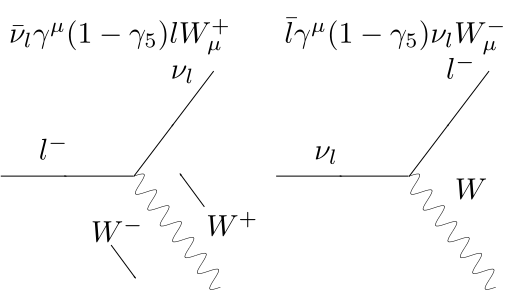
\includegraphics[scale=0.5]{leptoncc}
\qquad  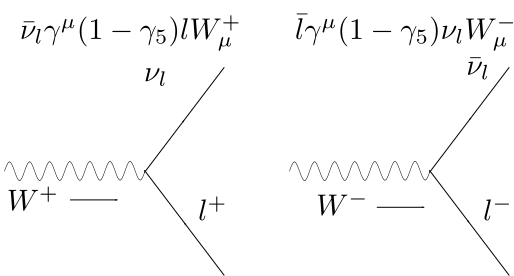
\includegraphics[scale=0.5]{wdecay}

  \caption{Diagramas de Feynman para las corrientes cargadas}
  \label{fig:leptoncc}
\end{figure}
Del primer y cuarto diagrama obtenemos el diagrama de Feynman para el decaimiento $\mu^-\to \nu_\mu e^-\bar{\nu}_e$, mostrado en la figura~\ref{fig:muondecay}
\begin{figure}
  \centering
  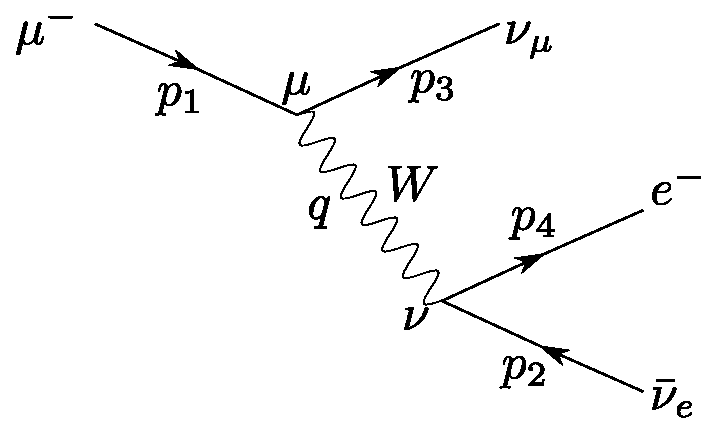
\includegraphics[scale=0.5]{muon_decay}
  \caption{diagrama de Feynman para el decaimiento $\mu^-\to \nu_\mu e^-\bar{\nu}_e$}
  \label{fig:muondecay}
\end{figure}
El propagador para el bosón $W$ de momentum $q$ resulta ser
\begin{align}
  \widetilde{D}_{\mu\nu}=\frac{1}{q^2-m_W^2}\left(g_{\mu\nu}-\frac{q_\mu q_\nu}{m_W^2}\right)\,.
\end{align}
Para los propósitos actuales la obtención de este resultado no es necesaria, el punto importante es que cuando las masas de las partículas iniciales y finales son mucho más pequeñas que $m_W$, esto se reduce a
\begin{align}
  \widetilde{D}_{\mu\nu}=-\frac{g_{\mu\nu}}{m_W^2}\,.
\end{align}
Este resultado se entiende fácilmente cuando se compara con el propagador de una partículas escalar masiva $1/(q^2-M^2)\to-1/M^2$. Las componentes espaciales de $W_\mu$ con $\mu=1,2,3$, a bajas energías tienen el mismo propagador que el de una partícula escalar, mientras $W_0$, tiene el signo opuesto.

El Lagrangiano efectivo para el decaimiento del muón, $\mu^-\to \nu_\mu e^- \bar{\nu}_e$ es entonces
\begin{align}
  \mathcal{L}=&\frac{g^2}{8}\left[\bar{\nu}_\mu\gamma^\mu(1-\gamma_5)\mu\right]\frac{g_{\mu\nu}}{m_W^2}
  \left[\bar{e}\gamma^\nu(1-\gamma_5)\nu_e\right]\nonumber\\
=&\frac{g^2}{8m_W^2}\left[\bar{\nu}_\mu\gamma^\mu(1-\gamma_5)\mu\right]
  \left[\bar{e}\gamma^\nu(1-\gamma_5)\nu_e\right]\nonumber\\
  =&\frac{G_F}{\sqrt{2}}\left[\bar{\nu}_\mu\gamma^\mu(1-\gamma_5)\mu\right]\left[\bar{e}\gamma_\mu(1-\gamma_5)\nu_e\right]\,,
\end{align}
donde
\begin{align}
  \frac{G_F}{\sqrt{2}}=&\frac{g^2}{8m_W^2}\nonumber\\
  =&\frac{g^24}{8g^2v^2}\nonumber\\
  =&\frac{1}{2v^2}\,,
\end{align}
y
\begin{align}
  v=\left(\sqrt{2}G_F\right)^{-1/2}\,.
\end{align}


De otro lado, para el  decaimiento $\beta$, $n\to p e^- \bar{\nu}_e$, de acuerdo a la figura~\ref{fig:neutrondecay}, tenemos

\begin{align}
    \mathcal{L}=\frac{G_\beta}{\sqrt{2}}\left[\bar{p}\gamma^\mu(1-1.26\gamma_5)n\right]\left[\bar{e}\gamma_\mu(1-\gamma_5)\nu_e\right]\,.
\end{align}
\begin{figure}
  \centering
  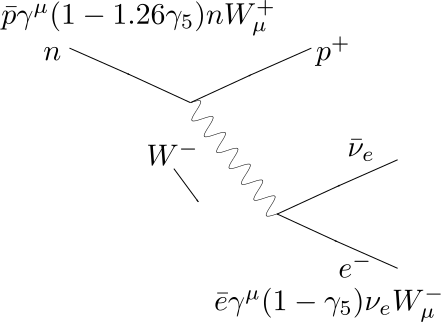
\includegraphics[scale=0.5]{neutrondecay}
  \caption{Decaimiento del neutrón.}
  \label{fig:neutrondecay}
\end{figure}
con $G_F$ dado en la ec.~\eqref{eq:233qft} y $G_\beta=1.10\timesm 10^{-5}\,\text{GeV}^2$. La corriente hadrónica tiene la forma V--1.26A. El factor 1.26  puede entenderse como debido a las correcciones a nivel hadrónico de una corriente que es de la forma V--A a nivel del quarks, como en la ec.~\eqref{eq:234qft}. A nivel de quarks el decaimiento del neutrón ($udd$) al protón ($uud$) corresponde al decaimiento de uno de los quarks down del neutrón $d\to u e^- \bar{\nu}_e$
\begin{align}
    \mathcal{L}=\frac{G_F}{\sqrt{2}}V_{11}\left[\bar{u}\gamma^\mu(1-\gamma_5)d\right]\left[\bar{e}\gamma_\mu(1-\gamma_5)\nu_e\right]\,.
\end{align}
De modo que $G_\beta=G_F V_{11}=G_F\cos\theta_C$, donde $\theta_C$ es el ángulo de Cabbibo. Una vez se tienen en cuenta correcciones electrodébiles se obtiene el valor $|V_{11}|=0.97418(27)$\cite{PDG}. Las magnitudes de los elementos de la matriz CKM son\cite{PDG}
\begin{align}
  V\approx\begin{pmatrix}
    0.97419&0.2257&0.0359\\
    0.2256&0.97334&0.0415\\
    0.00874&0.0407&0.999133
  \end{pmatrix}\sim \mathbf{1}
\end{align}

\section{Cálculo de procesos}

%%% Local Variables: 
%%% mode: latex
%%% TeX-master: "beyond"
%%% End: 

\chapter{Computational QFT}

\begin{frame}
There are several tools which allows for the generation of models of particle physics models like LanHEP \cite{Semenov:2008jy} 
\begin{center}
  \url{http://theory.sinp.msu.ru/~semenov/lanhep.html},
\end{center}
or FeynRules \cite{Christensen:2008py}
\begin{center}
  \url{http://feynrules.phys.ucl.ac.be/}\,.
\end{center}

This kind of programs are able to generate the output required for other programs which make the calculation of Feynman diagrams and integration over multi-particle phase space. CalcHEP:
\begin{center}
  \url{http://theory.sinp.msu.ru/~pukhov/calchep.html}
\end{center}
for example, is able to calculate cross section and decays widths at tree level.

\end{frame}

In this chapter we will illustrate the use LanHEP+CalcHEP

\section{LanHEP}

\begin{frame}[fragile,allowframebreaks]{}
After download the source code from the \url{http://theory.sinp.msu.ru/~pukhov/calchep.html} to some \lstinline{DIR}, 
\begin{itemize}
\item Note that the \lstinline{tar.gz} file name depends on the current version. At the moment of this writing this was \lstinline{lhep311.tar.gz}. To directly download this file use:
\begin{lstlisting}
$ wget http://theory.sinp.msu.ru/~semenov/lhep311.tar.gz
\end{lstlisting}
where \lstinline{\$} is to indicate that the command is to be written in the shell of your Linux session\footnote{An introduction to scientific computing is at \url{http://gfif.udea.edu.co/cf} }.
To uncompress the file:\\
\begin{lstlisting}
  $ tar -zxvf DIR/lhep311.tar.gz
\end{lstlisting}

\item Go to the created directory
\begin{lstlisting}
  $ cd lanhep311
\end{lstlisting}

\item To compile and create the executable of the program (\lstinline{lhep}):\\
\begin{lstlisting}
$ make
\end{lstlisting}
\end{itemize}


The input of LanHEP are files were the Lagrangian of some model is written in a symbolic way. Then, the LanHEP executable process the input files and generates four outputfiles which are the input for the CalcHEP program. For example, in the LanHEP dir

\begin{lstlisting}
$ ./lhep stand.mdl
\end{lstlisting}
Here \lstinline{./lhep} command, search for the file in the defaul directory \lstinline{mdl/stand.mdl}. If there are no erros printed, for files are created:
\begin{lstlisting}
 ls *4.mdl
 func4.mdl  lgrng4.mdl  prtcls4.mdl  vars4.mdl
\end{lstlisting}
\end{frame}
%%%%%%%%

\section{CalcHEP}
\begin{frame}[fragile,allowframebreaks]{}
The installation of CalcHEP is similar. In Ubuntu you must be sure to have \lstinline{libx11-dev} package, in addion to the C and Fortran compilers:
\begin{lstlisting}
$ sudo apt-get install libx11-dev build-essential gfortran
\end{lstlisting}
In the CalcHEP directory:
\begin{lstlisting}
$ make
\end{lstlisting}

To use CalcHEP you must first create a directory with the required files. This is achieved with the CalcHEP command
\begin{lstlisting}
$ ./mkUsrDir YourModel
\end{lstlisting}
A directory \lstinline{YourModel} is created with several files and directories inside. By default, a \lstinline{models} directory is created with two set of \lstinline{.mdl} files, corresponding to two versions of the Standard Model:
\begin{lstlisting}
$ ls YourModel/models/
func1.mdl  lgrng1.mdl  prtcls1.mdl   vars1.mdl  
func2.mdl  lgrng2.mdl  prtcls2.mdl   vars2.mdl
\end{lstlisting}

From the \lstinline{YourModel} directory in CalcHEP, run the command
\begin{lstlisting}
./calchep
\end{lstlisting}
A new window must appear with the info of CalcHEP and the loaded models in \lstinline{YourModel/models}. To navigate through this window, use the arrows keys and the \lstinline{<ESC>} key to navigate back into the menus.  
\end{frame}

\section{LanHEP/CalcHEP}

\begin{frame}[fragile,allowframebreaks]{}
The sample \lstinline{.mdl} files in the \lstinline{mdl} directory of LanHEP must be modified in order to generate the proper CalcHEP input files. From the LanHEP directory
\begin{lstlisting}
$ mkdir sm
$ cd sm
$ wget --no-check-certificate \
   https://github.com/rescolo/LanHEP/raw/release/sm/sm.mdl
$ wget --no-check-certificate \
   https://github.com/rescolo/LanHEP/raw/release/sm/sm_tex.mdl

$ ../lhep sm.mdl
\end{lstlisting}
The four CalcHEP input files:
\begin{lstlisting}
func1.mdl  lgrng1.mdl  prtcls1.mdl   vars1.mdl  
\end{lstlisting}
are then created.

From CalcHEP directoty:
\begin{lstlisting}
$ ./mkUsrDir sm
$ cd sm/models
$ rm * 
\end{lstlisting}
then copy the \lstinline{*1.mdl} files to the \lstinline{sm/models}, and from the \lstinline{sm} CalcHEP directory run \lstinline{./calchep}.

In order to understand the structure of the LanHEP files consider the following skeleton:
\begin{lstlisting}[numbers=left,xleftmargin=1cm,numberstyle=\tiny,escapeinside={(*}{*)}]
model 'MODEL NAME'/N.
% The coments are either this way
/* or this other way */

use file_tex.

prtcprop pdg.

prtcformat fullname:'  Full Name  ',
           name:' P ',
           aname:' aP ',
           pdg:' number ',
           spin2, mass, width, color, aux,
           texname:'>  LaTeX P name  <',
           atexname:'>  LaTeX aP name < '.

parameter  VAR  = VALUE : 'Description'.

particle_type  
	particle/Antiparticle: ('name', property name=VALUE, ...).

lterm  	Write here the Lagrangian in a LaTeX--like format

prtcprop pdg:(Particle=PDF code,...).

SetEM(A,EE). %check charge conservation
CheckHerm.
\end{lstlisting}
In line 1, \lstinline{N} is an integer that will identify the four output files. The file in line 5 will contain the \LaTeX{} definitions of the used particles. In lines 7-15, the format of the table \lstinline{prtclN.mdl}, as required by CalcHEP, is defined: A new column with the PDG number for the particle.  In line 17, the general form to declarate a variable is established, while the lines 19-20 are the generic declaration for a particle. The final commands in 26 and 27 is to check the consistency of the defined model. 
As a simple illustration consider the simple case of QED:
\begin{lstlisting}
model 'QED: e, mu tau'/1.

use qed3g_tex.

prtcprop pdg.

%prtc1.mdl is one of the output files of LanHEP. To make
% it compatible with CalcHEP we need to change their format
% to include the PDG particle number in the third column
 
prtcformat fullname:'  Full Name  ',
           name:' P ',
           aname:' aP ',
           pdg:' number ',
           spin2, mass, width, color, aux,
           texname:'>  LaTeX P name  <',
           atexname:'>  LaTeX aP name < '.

parameter  EE  = 0.31333 : 'Electromagnetic coupling constant (<->1/128)'.

vector  
	A/A: (photon, gauge).

spinor 		e1:(electron),
		e2:(muon, mass Mm  = 0.1057),
		e3:('tau-lepton', mass Mt  = 1.777).

% fermion interaction with gauge fields

lterm  	anti(psi)*gamma*(i*deriv - EE*A)*psi
		where 
			psi=e1;
			psi=e2;
			psi=e3.

% gauge bosons Lagrangian

lterm -F**2/4   where 
	F=deriv^mu*A^nu-deriv^nu*A^mu.

%set PDG particle numbers:

prtcprop pdg:(A=22,e1=11, e2=13, e3=15).

SetEM(A,EE). %check charge conservation
CheckHerm.
\end{lstlisting}
where the required file \lstinline{qed3g_tex.mdl} is
\begin{lstlisting}
SetTexName([e1=e,E1='\\bar{e}']).
SetTexName([e=e,E='\\bar{e}']).
SetTexName(['e1.c'='e^c','E1.c'='\\bar{e}^c']).
SetTexName(['e.c'='e^c','E.c'='\\bar{e}^c']).
SetTexName([e2='\\mu',E2='\\bar{\\mu}']).
SetTexName([e3='\\tau',E3='\\bar{\\tau}']).
SetTexName([m='\\mu',M='\\bar{\\mu}']).
SetTexName([l='\\tau',L='\\bar{\\tau}']).

SetTexName([EE=e]).

SetTexName([Me='M_e', Mm='M_\\mu', Mt='M_\\tau']).
\end{lstlisting}

Running with the option \lstinline{-tex}:
\begin{lstlisting}
../lhep qed3g.mdl
\end{lstlisting}
the following output is generated
\begin{itemize}
\item \lstinline{lgrng1.tex}
\begin{center}

\begin{tabular}{|l|l|} \hline
Fields in the vertex & Variational derivative of Lagrangian by fields \\ \hline
$\bar{e}{}_{a }$ \phantom{-} $e{}_{b }$ \phantom{-} ${A}_{\mu }$ \phantom{-}  &
        $- e\cdot \gamma_{a b}^\mu $\\[2mm]
$\bar{\mu}{}_{a }$ \phantom{-} $\mu{}_{b }$ \phantom{-} ${A}_{\mu }$ \phantom{-}  &
        $- e\cdot \gamma_{a b}^\mu $\\[2mm]
$\bar{\tau}{}_{a }$ \phantom{-} $\tau{}_{b }$ \phantom{-} ${A}_{\mu }$ \phantom{-}  &
        $- e\cdot \gamma_{a b}^\mu $\\ \hline
\end{tabular}

\end{center}



\item \lstinline{prtcls1.tex}:
  \begin{center}
    \begin{tabular}{|cc|l|c|c|c|l|} \hline
P & aP & Name & Spin  & EM charge & Color & Comment \\ \hline
$A_{\mu }$&$A_{\mu }$&photon        &1           & $\phantom{-}0$ &1    &gauge\\
$e{}_{a}$ &$\bar{e}{}_{a}$&electron      &$1/2$       &$\phantom{-}1$ &1    &   \\
$\mu{}_{a}$&$\bar{\mu}{}_{a}$&muon          &$1/2$       &$\phantom{-}1$ &1    &   \\
$\tau{}_{a}$&$\bar{\tau}{}_{a}$&tau-lepton    &$1/2$       &$\phantom{-}1$ &1    &   \\ \hline
\end{tabular}
  \end{center}

\item \lstinline{vars1.tex}
  \begin{center}
    \begin{tabular}{|l|l|l|} \hline
Parameter & Value & Comment \\ \hline
EE    &0.31333             &Electromagnetic coupling constant (1/128) \\
Mm    &0.1057              &mass of muon \\
Mt    &1.777               &mass of tau-lepton \\ \hline
\end{tabular}
  \end{center}
\end{itemize}

With the command
\begin{lstlisting}
$ ../lhep qed3g.mdl
\end{lstlisting}
the same files are generated by in the format of CalcHEP.

In CalcHEP
\begin{lstlisting}
$ ./mkUsrDir qed3g
$ cd qed3g/models
$ rm *
#copy the files: func1.mdl, lgrng1.mdl prtcls1.mdl, vars1.mdl here
$ cd ..
$ ./calchep
\end{lstlisting}
The window in Fig.~\ref{fig:calchep1}
\begin{figure}
  \centering
  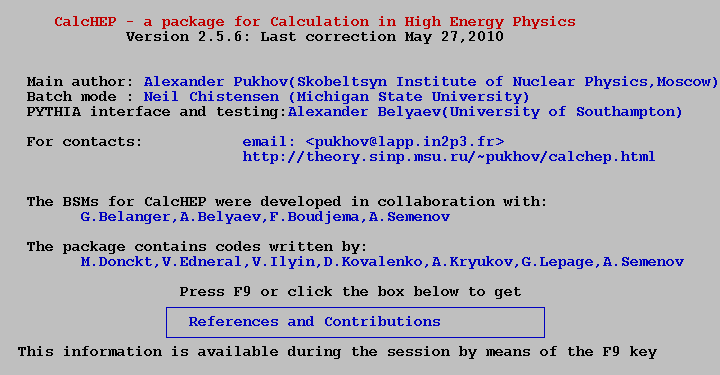
\includegraphics[scale=0.45]{calchep1}
  \caption{CalcHEP welcome window}
  \label{fig:calchep1}
\end{figure}
After hit \lstinline{<Enter>}, the window with the model should appears as shown in Fig.~\ref{fig:calchep2}
\begin{figure}
  \centering
  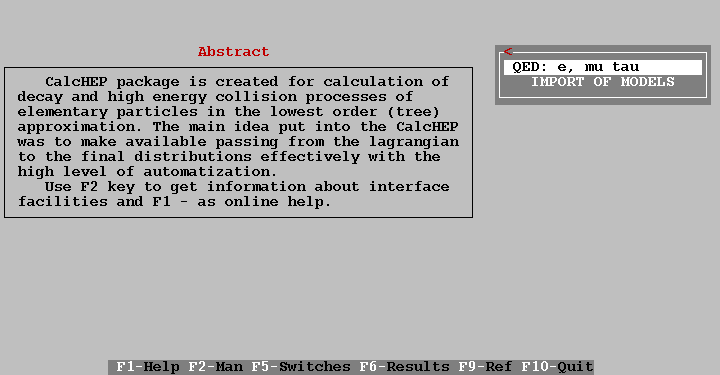
\includegraphics[scale=0.45]{calchep2}
  \caption{CalcHEP model window}
  \label{fig:calchep2}
\end{figure}
To test that the model was loaded without errors:
\begin{lstlisting}
QED: e, mu tau -> Edit Model -> Check Model
\end{lstlisting}
A message with \lstinline{The model is OK}, should popup.

After returning to the model window in Fig.~\ref{fig:calchep2}, we could calculate some process:
\begin{lstlisting}
QED: e, mu tau -> Enter Process 
\end{lstlisting}
and enter the process \lstinline{e1,E1 -> e2,E2} ($e^+ e^-\to \mu^+\mu^-$) as shown in the Fig:~\ref{fig:calchep3}
\begin{figure}
  \centering
  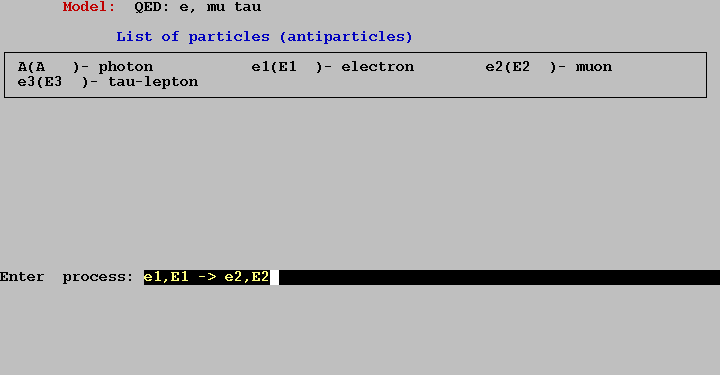
\includegraphics[scale=0.45]{calchep3}
  \caption{CalcHEP process window}
  \label{fig:calchep3}
\end{figure}
After \lstinline{<Enter>}, the window to calculate the process should appears, as in Fig.~\ref{fig:calchep4}
\begin{figure}
  \centering
  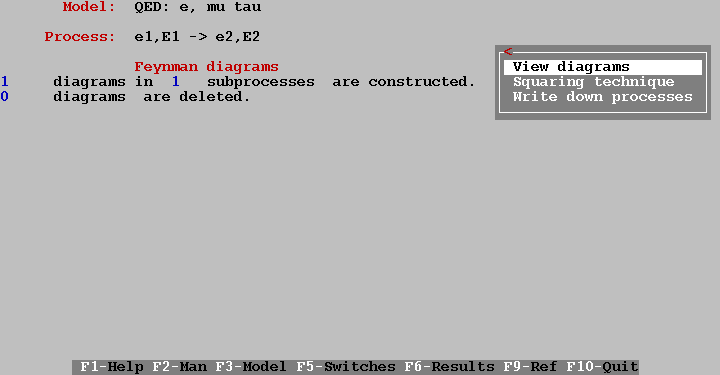
\includegraphics[scale=0.45]{calchep4}
  \caption{CalcHEP calculation window}
  \label{fig:calchep4}
\end{figure}
In addition to \lstinline{View diagrams}, we can calculate the process with the sequence
\begin{lstlisting}
Squaring technique -> Symbolic calculations -> C-compiler
\end{lstlisting}
Then a new window with the process details should appears, as displayed in Fig.~\ref{fig:calchep5}
\begin{figure}
  \centering
  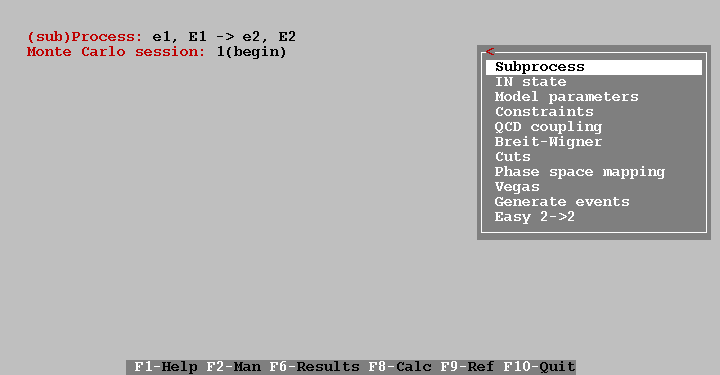
\includegraphics[scale=0.45]{calchep5}
  \caption{CalcHEP calculation window}
  \label{fig:calchep5}
\end{figure}
After adjust the input parameters at your convenience, we could just calculate the process with, in this case: \lstinline{Easy 2-2}, to obtain the result displayed in ~\ref{fig:calchep6}
\begin{figure}
  \centering
  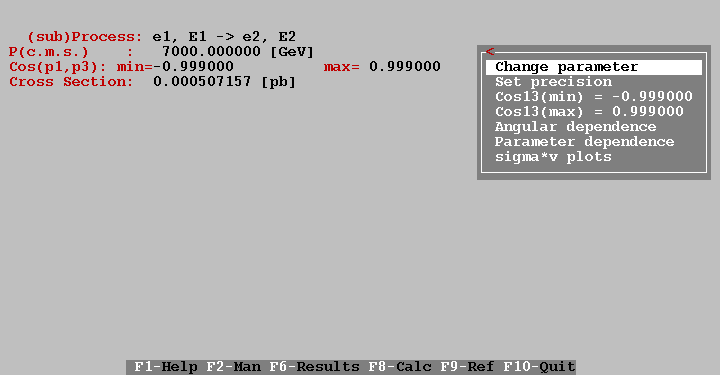
\includegraphics[scale=0.45]{calchep6}
  \caption{CalcHEP results window}
  \label{fig:calchep6}
\end{figure}
e.g, for center of mass energy of 14 TeV (7 TeV per beam) we could have:
\begin{align}
  \sigma(e^+\,e^-\to \mu^+\mu^-)=5\times 10^{-4}\,\text{pb}\,
\end{align}
\begin{itemize}
\item \textbf{Exercise}:
Repeat the previous calculation, but for one center of mass energy of 200 GeV.
\end{itemize}

For the Standard Model the Yukawa Lagrangian that couple the down fermions with the boson scalar is written in the interaction basis:
\begin{equation}\label{base_in}
  \mathcal{-L}_Y\sim\overline{D'}M_D P_R D'H + {\rm h.c}\; ,
\end{equation}
with $D'=V^{\dagger}D$, we can write the equation \ref{base_in} in the mass eigenstates 
as $\mathcal{-L}_Y\sim\overline{D}M_D^{dia}P_RDH + {\rm h.c}$ , where
\begin{equation}\label{masa_matrix}
  M_D^{dia}=VM_DV^{\dagger}
\end{equation}
 Investing the equation \ref{masa_matrix} and replacing in \ref{base_in} we can write in the interaction eigenstates:
$\mathcal{-L}_Y\sim \overline{D'}V^{\dagger}M_D^{dia}VP_R D'H + {\rm h.c}$, define $M'_D=M_D^{dia}V$ and $q'=VD'$ 
\footnote{$\overline{D'}V^{\dagger}=D'V^{\dagger}\gamma_0=(\gamma_0VD')^{\dagger}=(\gamma_0q')^{\dagger}=\overline{q'}$.}, therefore, the 
Yukawa Lagrangian in the interaction basis is:
\begin{equation}
  \mathcal{-L}_Y\sim\overline{q'}M_D' P_R D'H + {\rm h.c}\; .
\end{equation}




\end{frame}

%%% Local Variables: 
%%% mode: latex
%%% TeX-master: "beyond.beamer.tex"
%%% End: 


%%% Local Variables: 
%%% mode: latex
%%% TeX-master: "beyond"
%%% End:
%instiki:category: QuantumFieldTheory
\chapter{Second quantization}
\label{cha:second-quantization} %noinstiki
%instiki:
%instiki:***
%instiki:
%instiki:[[Beyond|Contents]]
%instiki:
%instiki:***
%instiki:
%instiki:* [Fock space for real scalar fields](#fock-space-real)
%instiki:
%instiki:* [Quantization of Fermions](#quant-ferm)
%instiki:


Two key ingredients to formulate the Quantum Field Theory (QFT) are the quantization of systems in which the particles can be created and destroyed (quamtum theory of radiation) and the behavior of relativistic systems. When both ingredients are present the particles can be understood as the excited modes of certain field. When the particles in a system are not relativistic, the formalism of creation and annihilation operators is just an alternative method to describe the Hamiltonian of the Schr\"odinger equation. In relativistic systems however, the existence of negative energy states force the construction of new quantum states, the Fock states, in order to have proper defined probabilities for the states of the system. In section xx we start by building the Fock states associated to a massless not relativistic scalar field. Then we generalize the results to a massive scalar field satisfying the Klein-Gordon equation.

Some parts of the discussion were based in some topics of chapters 4-6 of \cite{Maggiore:2005qv}.


In general, the formalism of second quantization is usefull to describe the states of an undetermined number of particles and interactions which do not conserve particle number. In addition to high-energy physics where any number of particles may be created or annihilated during a collision process, in statistitical physics it becomes useful to describe a macroscopic body using the grand-canonical statistical ensemble, in which the number of particles is allowed to fluctuate. In condensed-matter states the interactions may modify also the number of various excitation quanta, such as phonons. A more general formalism to discuss this systems is developed in Appendix~\ref{cha:green-functions}.

\section{Quantization of the nonrelativistic string}
\label{sec:fock-space-real}

\subsection{The clasical string}
\label{sec:clasical-string}
\begin{frame}[fragile,allowframebreaks]
In conventional quantization the energy of one state is interpreted as the possible eigenstates of an Hamiltonian operator acting on the states of the system. 
\begin{align}
  \widehat{H}|\text{State}\rangle=E|\text{State}\rangle
\end{align}
One step further is to consider the wave function as the eigenstate  of the operator--field acting on certain \emph{Fock states}
\begin{align}
\label{eq:1}
  \widehat{\Phi}|\text{Fock State}\rangle=\Phi||\text{Fock State}\rangle\,,
\end{align}
Like that usual quantum mechanical observable, the wave function will have an uncertainty. 
The Fock states are the states under which the classical wave function can be obtained with a small uncertainty
\begin{align}
    \Phi\pm\Delta\Phi=\langle\text{Fock State}|\widehat{\Phi}|\text{Fock State}\rangle
\end{align}
This happens when the number of quanta of the Fock state is big enough. In fact, a state with a definite number of quanta has a infinity uncertainty \cite{Gross:1993}.

Eq.~\eqref{eq:1} is the basis for the calculation of cross section and decay widths in quantum field theory. Now we will study how to define a such Fock state for a scalar field.


We have already see in Chapter 1 of \cite{lsm} that a string have a collective wave motion that is described by a continuous field, which satisfies the familiar one-dimensional wave equation
\begin{align}
\label{eq:2}
  \frac{1}{v^2}\frac{\partial^2\phi}{\partial t^2}-\frac{\partial^2\phi}{\partial z^2}=0
\end{align}
This equation can be derived following two different paths. The first is to decomposing the string into individual oscillators for which the usual Lagrangian formalism can be used. The second is just by formulating certain Lagrangian density from which the equation of motion can be obtained  by using the Euler-Lagrange equation
\begin{align}
  \partial_\mu\left[\frac{\partial\mathcal{L}}{\partial(\partial_\mu\phi)}\right]-\frac{\partial\mathcal{L}}{\partial\phi}=0\,.
\end{align}
In the first approach the string is considered to be composed of $N$ oscillators coupled together  by springs with a spring constant $k$. At certain time $t$, the displacement of the oscillator $i$ at time $t$ is represented by $\phi_i(t)$. In Table~\ref{tab:1} it is displayed the corresponding macroscopic quantities. Note also that $1/v^2=\mu/T$.
\begin{table}[htp!]
  \centering
  \begin{tabular}{l|l}
    micro & macro \\\hline{}
    $l$ & $L=N l$\\
    $m$ & $\mu=m/l$ \\
    $k$ & $T=k l$\\
    $\phi_i(t)=\phi(z_i,t)$ &  $\phi(z,t)$\\
  \end{tabular}
  \caption{From micro to macro}
\label{tab:1}
\end{table}
It is worth to stress that at the Lagrangian level, which is the sum of each individual oscillator Lagrangian, it is the sum of the kinetic and potential oscillator energy. However, the Lagrangian density only have the kinetic term for the scalar field
\begin{align}
  \mathcal{L}&=\frac{1}{2}\left(\frac{1}{v^2}\partial^0\phi\partial_0\phi+\partial^3\phi\partial_3\phi\right)\nonumber\\
  &\underset{v\to c=1}{\longrightarrow}\;\tfrac{1}{2}\partial^\mu\phi\partial_\mu\phi\,.
\end{align}
Note that only in the case $v=c$ this Lagrangian can be written in a covariant form. Moreover, the scalar field $\phi(z,t)$ have nothing to do with the individual oscillators. An specific solution for $\phi(z,t)$ would represent one specific oscillation mode of the string. It turn out that  this specific frequency mode corresponds to an particle state, that does have not connection with the physical particles in the string. 

The most general discrete solution to the wave equation  \eqref{eq:2} is the Fourier decomposition
\begin{align}
  \label{eq:3}
  \phi(t,z)=\sum_{n}\frac{v}{\sqrt{2\omega_{n} L}}
  \left(a_{n} e^{-i (\omega_n t-k_nz) }+a_{n}^* e^{i (\omega_n t-k_n z) }\right)
\end{align}
where the dispersion relation is
\begin{align}
\label{eq:4}
  \omega_n^2=v^2 k_n^2
\end{align}
where $\omega_n$ is definite positive:
\begin{align}
  \omega_n=+|v|\sqrt{|k_n|}
\end{align}

To satisfy the boundary conditions we must have
\begin{align}
  \label{eq:5}
  k_n=\frac{2\pi n}{L}
\end{align}
Note that
\begin{align}
  k_{-n}=-k_n\,.
\end{align}
Therefore
\begin{align}
  \omega_{-n}=\omega_n\,.
\end{align}
In three dimensions and with $v=c=1$, the Lagrangian can be written as
\begin{align}
\mathcal{L}=  \tfrac{1}{2}\partial^\mu\phi\partial_\mu\phi
\end{align}
This Lagrangian is still covariant after the addition of a function of $\phi$. An interesting case is just the addition of the mass term
the most general solution to the Klein--Gordon equation is 
\begin{align}
\mathcal{L}=  \tfrac{1}{2}\partial^\mu\phi\partial_\mu\phi-\tfrac{1}{2}m^2\phi^2
\end{align}
which give to arise to Klein-Gordon 
\begin{align}
  \left(\partial_\mu\partial^\mu-m^2\right)\phi=0\,.
\end{align}
We now will check the origin of the normalization factor. For simplicity we work with one spatial dimension. By using eq.~\eqref{eq:3}
\begin{equation}
\label{eq:6}
   \phi(z,t)=\sum_{n=-\infty}^\infty 
    \frac{v}{\sqrt{2\omega_n}}
  \left[a_n\,\phi_n(z,t)+a_n^*\,\phi_n^*(z,t)\right],
\end{equation}
\begin{align}
  [E]=&\frac{1}{[E]^{1/2}[E]^{-1}}[a]\nonumber\\
  =&E^{1/2}[a]
\end{align}
\begin{align}
  [a]=[E]^{1/2}
\end{align}
we define
\begin{align}
  \phi_n(z,t)=\frac{1}{\sqrt{L}}e^{-i(\omega_n t-k_n z)}
\end{align}

y las funciones $\phi_n$ satisfacen las siguientes condiciones de normalizaci\'on
\begin{align}
  \int_0^Ldz\,\phi_n^*(z,t)\phi_m(z,t)=&\frac{1}{L}\int_0^Ldz\,e^{i(\omega_n t-k_n z)}e^{-i(\omega_m t-k_m z)}\nonumber\\
=&\frac{1}{L}\int_0^Ldz\,\exp\{i[(\omega_n-\omega_m) t-(k_n-k_m) z]\}\nonumber\\
=&\frac{e^{i(\omega_n-\omega_m)t}}{L}\int_0^Ldz\,e^{-i(k_n-k_m) z}\nonumber\\
\end{align}
When $n=m$
\begin{align}
    \int_0^Ldz\,\phi_n^*(z,t)\phi_m(z,t)=&\frac{1}{L}\int_0^Ldz\nonumber\\
    =&1
\end{align}
For $n\neq m$, $2(n-m)$ is an even integer and then
\begin{align}
   \int_0^Ldz\,\phi_n^*(z,t)\phi_m(z,t)  =&\frac{e^{i(\omega_n-\omega_m)t}}{L}\left.
\frac{e^{-i(k_n-k_m) z}}{-i(k_n-k_m)}\right|_0^L\nonumber\\
=&\frac{e^{i(\omega_n-\omega_m)t}}{L}\frac{1}{-i(k_n-k_m)}
\left(e^{-i2\pi(n-m) }-1\right)\nonumber\\
=&0
\end{align}
In this way
\begin{equation}
\label{eq:7}
  \int_0^Ldz\,\phi_n^*(z,t)\phi_m(z,t)=\delta_{nm}.
\end{equation}
Moreover
\begin{equation}
\label{eq:8}
  \int_0^Ldz\,\phi_n(z,t)\phi_m(z,t)=\delta_{n,-m}e^{-2i\omega_nt}.
\end{equation}

En tal caso de 
\begin{equation}
  \label{eq:9}
  H=\int_{0}^{L}\mathcal{H}\,dz\,.
\end{equation}
From the analysis of the Theorem of Noether in chapter~1 of \cite{lsm} we have, that in a similar way to the usual Lagrangian formulation, where the canonical conjugate  variable is used to define the Legendre transformation
\begin{align}
  \label{eq:10}
  H=p \dot q-L\,,
\end{align}
the Hamiltonian density can be obtained from the Lagragian density trough the Legendre transformation
\begin{align}
\mathcal{H}&=T^0_0=\frac{\partial\mathcal{L}}{\partial\dot{\phi}}\dot{\phi}
      -\mathcal{L}\\
      &=\Pi(x)\frac{\partial\phi(x)}{\partial t}-\mathcal{L}.
\end{align}
where
\begin{equation}
\label{eq:11}
  \Pi(x)=\frac{\partial\mathcal{L}}{\partial(\partial\phi(x)/\partial t)}
\end{equation}
is the canonical conjugate variable (conjugate momentum) of  the canonical variable $\phi(x)$.

We have then,
\begin{align}
\label{eq:12}
  H&=\frac{1}{2v^2}\int_0^Ldz\,\frac{\partial\phi}{\partial t}\frac{\partial\phi}{\partial t}+
  \frac{1}{2}\int_0^Ldz\,\frac{\partial\phi}{\partial z}\frac{\partial\phi}{\partial z}\nonumber\\
&=\sum_{n=-\infty}^\infty\omega_n\,a_n^*a_n
\end{align}
Demostration:
\begin{align}
  \frac{\partial\phi}{\partial t}=&\sum_{n=-\infty}^\infty \frac{v}{\sqrt{2\omega_n}}
  \left[-i\omega_n a_n\,\phi_n(z,t)+i\omega_n a_n^*\,\phi_n^*(z,t)\right],\nonumber\\
=&\sum_{n=-\infty}^\infty\frac{-i v\omega_n}{\sqrt{2\omega_n}}
  \left[a_n\,\phi_n(z,t)- a_n^*\,\phi_n^*(z,t)\right],
\end{align}
\begin{align}
\frac{1}{v^2}   \frac{\partial\phi}{\partial t} \frac{\partial\phi}{\partial t}=&
\sum_{n,m=-\infty}^\infty\frac{- \omega_n\omega_m}{2\sqrt{\omega_n\omega_m}}
  \left[a_n\,\phi_n(z,t)- a_n^*\,\phi_n^*(z,t)\right]
\left[a_m\,\phi_m(z,t)- a_m^*\,\phi_m^*(z,t)\right]\\
=  &
\sum_{n,m=-\infty}^\infty\frac{- \omega_n\omega_m}{2\sqrt{\omega_n\omega_m}}
  \left[a_n a_m \phi_n \phi_m- a_n^*a_m\phi_n^*\phi_m-a_n a_m^* \phi_n \phi_m^*+ a_n^*a_m^*\phi_n^*\phi_m^*\right]
\end{align}

\begin{align}
  \frac{\partial\phi}{\partial z}=&\sum_{n=-\infty}^\infty \frac{v}{2\sqrt{\omega_n}}
  \left[ik_n a_n\,\phi_n(z,t)-ik_n a_n^*\,\phi_n^*(z,t)\right],\nonumber\\
=&\sum_{n=-\infty}^\infty\frac{i vk_n}{2\sqrt{\omega_n}}
  \left[a_n\,\phi_n(z,t)- a_n^*\,\phi_n^*(z,t)\right],
\end{align}
\begin{align}
   \frac{\partial\phi}{\partial z} \frac{\partial\phi}{\partial z}=&
\sum_{n,m=-\infty}^\infty\frac{-v^2 k_nk_m}{2\sqrt{\omega_n\omega_m}}
  \left[a_n\,\phi_n(z,t)- a_n^*\,\phi_n^*(z,t)\right]
\left[a_m\,\phi_m(z,t)- a_m^*\,\phi_m^*(z,t)\right]\\
=  &
\sum_{n,m=-\infty}^\infty\frac{- v^2k_nk_m}{2\sqrt{\omega_n\omega_m}}
  \left[a_n a_m \phi_n \phi_m- a_n^*a_m\phi_n^*\phi_m-a_n a_m^* \phi_n \phi_m^*+ a_n^*a_m^*\phi_n^*\phi_m^*\right]
\end{align}
Using eqs.~\eqref{eq:7}, and \eqref{eq:8}
\begin{align}
  H=  &\frac12
\sum_{n,m=-\infty}^\infty\int_0^Ldz\frac{- \omega_n\omega_m}{2\sqrt{\omega_n\omega_m}} 
  \left[a_n a_m \phi_n \phi_m- a_n^*a_m\phi_n^*\phi_m-a_n a_m^* \phi_n \phi_m^*+ a_n^*a_m^*\phi_n^*\phi_m^*\right]\nonumber\\
&+\frac12\sum_{n,m=-\infty}^\infty\int_0^Ldz \frac{- v^2k_nk_m}{2\sqrt{\omega_n\omega_m}}
  \left[a_n a_m \phi_n \phi_m- a_n^*a_m\phi_n^*\phi_m-a_n a_m^* \phi_n \phi_m^*+ a_n^*a_m^*\phi_n^*\phi_m^*\right]\nonumber\\
  =  &\frac12
\sum_{n,m=-\infty}^\infty\frac{- \omega_n\omega_m}{2\sqrt{\omega_n\omega_m}} 
  \left[a_n a_m \delta_{n,-m}e^{-2i\omega_n t}- a_n^*a_m\delta_{n, m}-a_n a_m^* \delta_{n,m}+ a_n^*a_m^*\delta_{n,-m}e^{2i\omega_n t}\right] \nonumber\\
  &+\frac12
\sum_{n,m=-\infty}^\infty\frac{-v^2 k_nk_m}{2\sqrt{\omega_n\omega_m}} 
  \left[a_n a_m \delta_{n,-m}e^{-2i\omega_n t}- a_n^*a_m\delta_{n, m}-a_n a_m^* \delta_{n,m}+ a_n^*a_m^*\delta_{n,-m}e^{2i\omega_n t}\right]\nonumber\\
  =  &\frac12
\sum_{n=-\infty}^\infty 
  \left[\frac{- \omega_n\omega_{-n}}{2\sqrt{\omega_n\omega_{-n}}}a_n a_n e^{-2i\omega_n t}
+\frac{ \omega_n\omega_n}{2\sqrt{\omega_n\omega_n}}(a_n^*a_n+a_n a_n^*)- \frac{\omega_n\omega_{-n}}{2\sqrt{\omega_n\omega_{-n}}} a_n^*a_{-n}^*e^{2i\omega_n t}\right]\nonumber\\
&+\frac12
\sum_{n=-\infty}^\infty 
  \left[\frac{-v^2 k_nk_{-n}}{2\sqrt{\omega_n\omega_{-n}}}a_n a_n e^{-2i\omega_n t}
+\frac{ k_nk_n}{2\sqrt{\omega_n\omega_n}}(a_n^*a_n+a_n a_n^*)- \frac{k_nk_{-n}}{2\sqrt{\omega_n\omega_{-n}}} a_n^*a_{-n}^*e^{2i\omega_n t}\right]
\end{align}

\end{frame}
\begin{frame}[fragile,allowframebreaks]
Since $\omega_n=\omega_{-n}$ and $k_n=-k_{-n}$
\begin{align}
 H =  &\frac12
\sum_{n=-\infty}^\infty \frac{1}{2\omega_n}
  \left[(- \omega_n^2+v^2 k_n^2)a_n a_n e^{-2i\omega_n t}
+( \omega_n^2+v^2 k_n^2)(a_n^*a_n+a_n a_n^*)\right.\nonumber\\
&+\left.(- \omega_n^2+v^2 k_n^2)a_n^*a_{-n}^*e^{2i\omega_n t}\right]
\end{align}
Finally, using eq.~\eqref{eq:4}
\begin{align}
\label{eq:13}
  H=\frac{1}{2}\sum_{n=-\infty}^\infty\omega_n(a_n^*a_n+a_n a_n^*)
\end{align}
Since $a_n$ and $a_n^*$ are classical quantities that commutates, the Hamiltonian is
\begin{align}
  \label{eq:14}
  H=\sum_{n=-\infty}^\infty\omega_na_n^*a_n=\sum_{n=-\infty}^\infty\omega_n|a_n|^2
\end{align}

In this way, the factor $\sqrt{2\omega_{n}}$ in eq.~\eqref{eq:6}, is a convenient choice of normalization for the coefficients $a_n$ which guarantees the Hamiltonian.

To quantize the string, we need to promote $H$ to an operator. In canonical quantization we need to identify the proper conjugates variables. For this purpose it is convenient to write eq.~\eqref{eq:14} as the Hamiltonian of an harmonic oscillator.
\end{frame}
\subsection{Quantization of the string}
\label{sec:quantization-string}
\begin{frame}[fragile,allowframebreaks]

This Hamiltonian can be rewritten as a sum of independent  oscillators Hamiltonians. Consider an harmonic oscillator of frequency $\omega$. The equation of motion for $F=-k q$ is
\begin{align}
  \ddot{q}+\frac{k}{m}q=&0\nonumber\\
   \ddot{q}+\omega^2q=&0
\end{align}
with
\begin{align}
  \omega^2=\frac{k}{m}
\end{align}
This equation of motion can be obtained from the Lagrangian
\begin{align}
  L=T-V=\frac{1}{2}[m\dot{q}^2-k q^2]
\end{align}
And the Hamiltonian can be obtained from eq.~\eqref{eq:10}
\begin{align}
   H=&p \dot{q}-L\nonumber\\
   =&\frac{p^2}{m}-\frac{1}{2}\frac{p^2}{m}+k q^2\nonumber\\
   =&\frac{1}{2}\left(\frac{p^2}{m}+m \omega^2 q^2\right)\nonumber\\
   =&\frac{1}{2m}\left({p^2}+m^2 \omega^2 q^2\right)\nonumber\\
\end{align}
For a set of independent oscillators we have
\begin{align}
\label{eq:15}
  H=&\sum_n\frac{1}{2m}\left({p_n^2}+m^2 \omega_n^2 q_n^2\right)\nonumber\\
  H=&\sum_n{\omega_n}\left(\frac{1}{{2m}\omega_n}p_n^2+\frac{m\omega_n}{2} q_n^2\right)
\end{align}
Comparing eq.~\eqref{eq:15} with Eq.~\eqref{eq:14} we see that the complex number $a_n$ can be written as ($\hbar=1$)
\begin{align}
  a_n=& c_1q_n+i c_2p_n
\end{align}

\begin{align}
  a_n^*a_n=c_1^2 q_n^2+c_2^2 p_n^2
\end{align}
\begin{align}
c_1=&\frac{\sqrt{m\omega_n}}{\sqrt{2}}=\frac{m\omega_n}{\sqrt{2m\omega_n}}   & c_2=&\frac{1}{\sqrt{2m\omega_n}}
\end{align}
\begin{align}
  a_n=&\frac{m\omega_n q_n+i\,p_n}{\sqrt{2m\omega_n}}\nonumber\\
  a_n^*=&\frac{m\omega_n q_n-i\,p_n}{\sqrt{2m\omega_n}}\nonumber\\
\end{align}
\begin{align}
a_n+a_n^*=& 2\frac{m\omega_n}{\sqrt{2m\omega_n}}q_n=\sqrt{2m\omega_n}q_n \Rightarrow& q_n=&\frac{1}{\sqrt{2m\omega_n}}(a_n+a_n^*) \nonumber\\
a_n-a_n^*=&\frac{2i}{\sqrt{2m\omega_n}}p_n=\frac{i\sqrt{2m\omega_n}}{m\omega_n}p_n
\Rightarrow& p_n=&-\frac{im\omega_n}{\sqrt{2m\omega_n}}(a_n-a_n^*) 
\end{align}
In quantum mechanics the classical objects $q_n$ and $p_n$ are promoted to operators which satisfy the commutation relation

\begin{align}
\label{eq:16}
  [\widehat{q}_n,\widehat{p}_m]=&i\delta_{m n} &
  [\widehat{q}_n,\widehat{q\,}_m^\dagger]= [\widehat{p_n},\widehat{p\,}_m^\dagger]=&0\,. 
\end{align}
This implies that the objects $a_n$ and $a_n^*$, are also operators
\begin{align}
  [\widehat{q}_n,\widehat{p}_m]=&-\frac{i m\omega_m}{\sqrt{2m\omega_n 2m\omega_m}}\{ 
[\widehat{a}_{n},\widehat{a}_{m}]-[\widehat{a}_{n},\widehat{a}_{m}^\dagger]
+[\widehat{a}_{n}^\dagger,\widehat{a}_{m}]+[\widehat{a}_{n}^\dagger,\widehat{a}_{m}^\dagger]
\} \nonumber\\
  [\widehat{q}_n,\widehat{p}_m]=&-\frac{i m\omega_m}{2\sqrt{m\omega_n m\omega_m}}\{ 
[\widehat{a}_{n},\widehat{a}_{m}]-2[\widehat{a}_{n},\widehat{a}_{m}^\dagger]
+[\widehat{a}_{n}^\dagger,\widehat{a}_{m}^\dagger]
\} 
\end{align}
If the operators $\widehat{a}_{n}$ and $\widehat{a}_{n}^\dagger$ satisfy the commutation relations
\begin{align}
\label{eq:17}
  &\left[\widehat{a}_{n},\widehat{a}_{m}^\dagger\right]=
\delta_{{n},{m}}&
&\left[\widehat{a}_{n},\widehat{a}_{m}\right]=
\left[\widehat{a}_{n}^\dagger,\widehat{a}_{m}^\dagger\right]=0\,,
\end{align}
then we recover equations \eqref{eq:16}. The scalar field is now an operator
\begin{align}
\label{eq:18}
  \widehat{\phi}=&\sum_{n=-\infty}^\infty\frac{v}{\sqrt{2\omega_nL}}
  \left[\widehat{a}_n\,e^{-i(\omega_n t-k_n z)}+\widehat{a\,}_n^\dagger\,e^{i(\omega_n t-k_n z)}\right],
\end{align}


In terms of operators $\widehat{a}_{n}$ and $\widehat{a\,}_{n}^\dagger$ the Hamiltonian from eq.~(\ref{eq:13}) can be written as
\begin{align}
\label{eq:129}
\widehat{H}=&\frac{1}{2}\sum_{n=-\infty}^{\infty} \omega_n (\widehat{a\,}_{n}^\dagger\widehat{a}_{n} +\widehat{a}_{n} \widehat{a\,}_{n}^\dagger)
\nonumber\\
=&\frac{1}{2}\sum_{n=-\infty}^{\infty} \omega_n \left(2\widehat{a\,}_{n}^\dagger\widehat{a}_{n} 
+\left[\widehat{a}_{n}, \widehat{a\,}_{n}^\dagger\right]\right)
\nonumber\\
=&\sum_{n=-\infty}^{\infty} \omega_n \left(\widehat{a\,}_{n}^\dagger\widehat{a}_{n} +\frac{1}{2}\right)
\end{align}
Since
\begin{align}
  \sum_{n=-\infty}^{\infty}\omega_n \frac{1}{2}\to\infty\,,
\end{align}
it is convenient to renormalize the Hamiltonian as
\begin{align}
\label{eq:130}
  \colon\!\widehat{H}\colon=&\sum_{n=-\infty}^{\infty} \omega_n \left(\widehat{a\,}_{n}^\dagger\widehat{a}_{n} +\frac{1}{2}\right)-
  \sum_{n=-\infty}^{\infty} \frac{1}{2}\nonumber\\
=&\sum_{n=-\infty}^{\infty} \omega_n \widehat{a\,}_{n}^\dagger\widehat{a}_{n}
\end{align}
This procedure is consistent since the related physics quantities arise from energy differences, no from absolute energy determinations.

  
\begin{align}
  \left[\widehat{H},\widehat{a}_{m}\right]=&
  \sum_{n=-\infty}^{\infty} \omega_n
  \left[\left(\widehat{a\,}_{n}^\dagger\widehat{a}_{n} +\frac{1}{2}\right),\widehat{a}_{m}\right]\nonumber\\
  =&\sum_{n=-\infty}^{\infty} \omega_n\left[\widehat{a\,}_{n}^\dagger\widehat{a}_{n},\widehat{a}_{m}\right]
\end{align}
By using the identity
\begin{align}
  \left[A B,C\right]=\left[A,C\right]B+A\left[B,C\right]
\end{align}
we have
\begin{align}
\label{eq:19}
   \left[\widehat{H},\widehat{a}_{m}\right]=&
\sum_{n=-\infty}^{\infty} \omega_n\left(
\left[\widehat{a\,}_{n}^\dagger,\widehat{a}_{m}\right]\widehat{a}_{n}
+\widehat{a\,}_{n}^\dagger\left[\widehat{a}_{n},\widehat{a}_{m}\right]
\right)\nonumber\\
=&-\sum_{n=-\infty}^{\infty} \omega_n
\delta_{n m}\widehat{a}_{n}
\nonumber\\
=&- \omega_m\widehat{a}_{m}
\end{align}

\begin{align}
\label{eq:20}
   \left[\widehat{H},\widehat{a\,}_{m}^\dagger\right]=&
\sum_{n=-\infty}^{\infty} \omega_n\left(
\left[\widehat{a\,}_{n}^\dagger,\widehat{a\,}_{m}^\dagger\right]\widehat{a}_{n}
+\widehat{a\,}_{n}^\dagger\left[\widehat{a}_{n},\widehat{a\,}_{m}^\dagger\right]
\right)\nonumber\\
=&\sum_{n=-\infty}^{\infty} \omega_n
\widehat{a\,}_{n}^\dagger\delta_{n m}
\nonumber\\
=& \omega_m\widehat{a\,}_{n}^\dagger
\end{align}

If $|m_n\rangle$ is an eigenstate of $\widehat{H}$ with eigenvalue $E_n$
\begin{align}
  \widehat{H}|m_n\rangle=E_n|m_n\rangle
\end{align}
then
\begin{align}
  \widehat{H}\,\widehat{a}_{n}|m_n\rangle=&
\left(\widehat{a}_{n}\widehat{H}-\omega_n\widehat{a}_{n}\right)|m_n\rangle\nonumber\\
=&\left(E_n-\omega_n\right)\widehat{a}_{n}|m_n\rangle\nonumber\\
\end{align}
$\widehat{a}_{n}|m_n\rangle$ is also an eigenstate with eigenvalue $E_n-\omega_n$. Moreover,
\begin{align}
  \widehat{H}\,\widehat{a\,}_{n}^\dagger|m_n\rangle=&
\left(\widehat{a\,}_{n}^\dagger\widehat{H}+\omega_n\widehat{a\,}_{n}^\dagger\right)|m_n\rangle\nonumber\\
=&\left(E_n+\omega_n\right)\widehat{a\,}_{n}^\dagger|m_n\rangle\nonumber\\
\end{align}
$\widehat{a\,}_{n}^\dagger|m_n\rangle$ is also an eigenstate with eigenvalue $E_n+\omega_n$. 

As stablished in \cite{Lahiri:2005sm}
\begin{quote}
  In other words, the operator $\widehat{a}_{n}$ seems to annihilate a quantum of energy, of amount $\hbar\omega_n$, from the state. On the other hand, 
  $\widehat{a\,}_{n}^\dagger$ creates a quantum of energy $\hbar\omega_n$. In this sense, they are the are the annihilation and the creation operators, respectively. [...]

The ground state can be denoted by $|0\rangle=|0_n\rangle$. Since this is state of lowest energy, the annihilation operator $\widehat{a\,}_{n}^\dagger$,
acting on it, cannot produce a state of lower energy. Thus, this state must be totally annihilated by the operation of $\widehat{a}_{n}$:
\begin{align}
  \widehat{a}_{n}|0\rangle=&0\nonumber\\
\langle0|\widehat{a\,}_{n}^\dagger=&0\,,
\end{align}
\end{quote}
such that
\begin{align}
  \langle0|0\rangle=1
\end{align}
The energy if the ground state can be fixed to zero:
\begin{align}
  :\widehat{H}:|0\rangle=0\,.
\end{align}

We define the state whose energy is larger tha the energy of $|0\rangle$ by one quantum $\hbar\omega_n$ by
\begin{align}  
  |1_n\rangle\equiv&\widehat{a\,}_{n}^\dagger|0\rangle\nonumber\\ 
  \langle1_n|=&\langle0|\widehat{a}_{n}
\end{align}

$|1_n\rangle$ is an Hamiltonian eigenstate of energy $\omega_n$:
\begin{align}
  :\widehat{H}:|1_n\rangle =&\omega_n a_n^\dagger a_n |1_n\rangle \nonumber\\ 
&=\omega_n|1_n\rangle\nonumber\\
&=\omega_n\cdot 1|1_n\rangle\,,
\end{align}
where we have made explicit that we have a quantum of energy $\hbar\omega$. The normalized state is
\begin{align}
  \langle1_n|1_n\rangle=&\langle0|\widehat{a}_{n}\widehat{a\,}_{n}^\dagger|0\rangle\nonumber\\
  =&\langle0|\left[\widehat{a}_{n},\widehat{a\,}_{n}^\dagger\right]|0\rangle\nonumber\\
  =&\langle0|0\rangle\nonumber\\
  =&1\,.
\end{align}
Similarly, the state with energy $2\hbar\omega$ is
\begin{align}
\frac{1}{\sqrt{2}} \left(\widehat{a\,}_{n}^\dagger\right)^2 |0\rangle=&|2_n\rangle\nonumber\\
  \langle0|\frac{1}{\sqrt{2}}\left(\widehat{a}_{n}\right)^2=&\langle2_n|
\end{align}
with normalization
\begin{align}
  \langle2_n|2_n\rangle=&\frac{1}{2}\langle0|\widehat{a}_{n}\widehat{a}_{n}\widehat{a\,}_{n}^\dagger\widehat{a\,}_{n}^\dagger|0\rangle\nonumber\\
=&\frac{1}{2}\langle1_n|\widehat{a}_{n}\widehat{a\,}_{n}^\dagger|1_n\rangle\nonumber\\
=&\frac{1}{2}\left(\langle1_n|\left[\widehat{a}_{n},\widehat{a\,}_{n}^\dagger\right]+\widehat{a\,}_{n}^\dagger\widehat{a}_{n}|1_n\rangle\right)\nonumber\\
=&\frac{1}{2}\left(\langle1_n|1_n\rangle+\langle0|0\rangle\right)\nonumber\\
  =&1\,.
\end{align}
By induction we get
\begin{align}
\label{eq:sp}
\frac{1}{\sqrt{m!}} \left(\widehat{a\,}_{n}^\dagger\right)^m |0\rangle=&|m_n\rangle
\end{align}
From here we have 

\begin{align}
\frac{1}{\sqrt{m!}} \widehat{a\,}_{n}^\dagger\left(\widehat{a\,}_{n}^\dagger\right)^{m-1} |0\rangle=&|m_n\rangle\nonumber\\
\frac{\sqrt{(m-1)!}}{\sqrt{m!}}\frac{1}{\sqrt{(m-1)!}} \widehat{a\,}_{n}^\dagger\left(\widehat{a\,}_{n}^\dagger\right)^{m-1} |0\rangle=&|m_n\rangle\nonumber\\
\sqrt{\frac{(m-1)!}{m(m-1)!}} \widehat{a\,}_{n}^\dagger|(m-1)_n\rangle=&|m_n\rangle\nonumber\\
\sqrt{\frac{1}{m}} \widehat{a\,}_{n}^\dagger|(m-1)_n\rangle=&|m_n\rangle\nonumber\\
 \widehat{a\,}_{n}^\dagger|(m-1)_n\rangle=&\sqrt{m}|m_n\rangle\nonumber\\
 \widehat{a\,}_{n}^\dagger|m_n\rangle=&\sqrt{m+1}|(m+1)_n\rangle
\end{align}
or,
\begin{align}
  \langle m_n|\widehat{a\,}_{n}=&\sqrt{m+1}\langle(m+1)_n|
\end{align}
From this expressions we can check that number operator can be defined from:
\begin{align}
 \langle m_n|\widehat{a\,}_{n}  \widehat{a\,}_{n}^\dagger|m_n\rangle=&(m+1)\langle(m+1)_n|(m+1)_n\rangle\nonumber\\
 \langle m_n|1+\widehat{a\,}_{n}^\dagger\widehat{a\,}_{n} |m_n\rangle=&(m+1)\nonumber\\
 \langle m_n|1+\widehat{\mathcal{N}}_n |m_n\rangle=&(m+1)
\end{align}
In this way, the number operator as
\begin{align}
  \widehat{\mathcal{N}}_n=\widehat{a\,}_{n}^\dagger\widehat{a}_{n}
\end{align}


If $\widehat{\mathcal{N}}_n|m_n\rangle=c|m_n\rangle$, where $c$ must be real because $\widehat{\mathcal{N}}_n$ is Hermitian
\begin{align}
  1+c=m+1
\end{align}
and
\begin{align}
  \widehat{\mathcal{N}}_n|m_n\rangle=m_n|m_n\rangle
\end{align}
From here, we can calculate the eigenvalues of $\widehat{a}_n$. Since
\begin{align}
\widehat{\mathcal{N}}_n\widehat{a}_n=&  
\left[\widehat{\mathcal{N}}_n,\widehat{a}_n\right]+
\widehat{a}_n\widehat{\mathcal{N}}_n\nonumber\\
=&\left[\widehat{a\,}_n^\dagger,\widehat{a}_n\right]\widehat{a}_n
+\widehat{a}_n\widehat{\mathcal{N}}_n
+\widehat{a\,}_n^\dagger\left[\widehat{a}_n,\widehat{a}_n\right]\nonumber\\
=&-\widehat{a}_n+\widehat{a}_n\widehat{\mathcal{N}}_n\nonumber\\
=&\widehat{a}_n\left(\widehat{\mathcal{N}}_n-1\right)
\end{align}
\begin{align}
  \widehat{\mathcal{N}}_n\widehat{a}_n|m_n\rangle=&(m_n-1)\widehat{a}_n|m_n\rangle
\end{align}
Since the state
\begin{align}
   \widehat{\mathcal{N}}_n|m_n-1\rangle=&(m_n-1)|m_n-1\rangle
\end{align}
has the same eigenvalue, therefore
\begin{align}
  \widehat{a}_n|m\rangle=C_-|m_n-1\rangle
\end{align}
where $C_-$ is a number to be determined from the normalization condition
\begin{align}
\label{eq:131}
   \langle m_n|\widehat{a\,}_{n}^\dagger\widehat{a\,}_{n}  |m_n\rangle=&
\left|C_-\right|^2\langle m_n-1|m_n-1\rangle\nonumber\\
   \langle m_n|\widehat{\mathcal{N}}_n|m_n\rangle=&
\left|C_-\right|^2\nonumber\\
\left|C_-\right|^2=m_n
\end{align}
\begin{align}
  \widehat{a}_n|m_n\rangle=\sqrt{m_n}|m_n-1\rangle
\end{align}


%\left[\right]

such that
\begin{align}
    \langle m_n|m_n\rangle=1
\end{align}
Eq.~\eqref{eq:130} can be rewritten as
\begin{align}
  \colon\!\widehat{H}\colon=&\sum_{n=-\infty}^{\infty} \omega_n \widehat{\mathcal{N}}_n
\end{align}
Noting also that
\begin{align}
  \mathcal{N}_n|m_l\rangle=0\qquad n\ne l\,, 
\end{align}
we have that
\begin{align}
  \langle m_n|\colon\!\widehat{H}\colon|m_n\rangle=m_n \omega_n=m_n \hbar\omega_n\,.
\end{align}
Therefore, once we have proper normalized states and renormalized Hamiltonian, the energy of an state with $m$ quantum ( of frequency $\omega_n$) is just $m$ times the energy of the one quanta of energy $\hbar\omega_n$. Note that
\begin{align}
  \langle 0|\colon\!\widehat{H}\colon|0\rangle=0\,.
\end{align}
The general procedure to redefine the zero of energy such that the vacuum energy vanishes is called \emph{normal ordering}. We define a normal-ordered product  by moving all annihilation operators to the right of all creation operators. For an operator $\widehat{X}$, its normal-ordered product will be denoted as $\colon\widehat{X}\colon$. Using this algorithm on the expression of eq.~\eqref{eq:129}, we find that
\begin{align}
\label{eq:133}
  \colon\widehat{H}\colon=&\frac{1}{2}\sum_{n=-\infty}^{\infty} \omega_n \colon(\widehat{a\,}_{n}^\dagger\widehat{a}_{n} +\widehat{a}_{n} \widehat{a\,}_{n}^\dagger)\colon\nonumber\\
=&\frac{1}{2}\sum_{n=-\infty}^{\infty} \omega_n (\widehat{a\,}_{n}^\dagger\widehat{a}_{n} +\widehat{a\,}_{n}^\dagger\widehat{a}_{n} )\nonumber\\
=&\sum_{n=-\infty}^{\infty} \omega_n \widehat{a\,}_{n}^\dagger\widehat{a}_{n}
\end{align}



From \cite{McMahon:2009zz} (pag. 121):
\begin{quote}
  These idea carry over to quantum field theory, but with a different interpretation. In quantum mechanics we are talking about a single particle state $|m_n\rangle$ and energy levels $E_n=\omega(n+1/2)$. The creation and annihilation operators move the state of the particle up and down in energy from the ground.

In quantum field theory, we take the notion of ``number operator'' literally. The state $|n\rangle$ is not a state of a single particle, rather is an state of the field with $N$ particles present. The background state which is also the lowest energy state is a state of the field with 0 particles (but the field is still there). The creation operator $\widehat{a\,}_n^\dagger$ adds a single quantum (a particle) to the field, while the annihilation operator $\widehat{a}_n$ destroys a single quantum (removes a single particle) from the field. As we will see, in general there will be creation operators and annihilation operators for particles as well as for antiparticles.

These operators will be functions of momentum. The fields will become operators which will be written as sums over annihilation and creation operators.
\end{quote}

%DEBUG: further development


\end{frame}



\subsection{Generalization to three dimensions}
\label{sec:gener-three-dimens}
\begin{frame}[fragile,allowframebreaks]
Taking into account that $E_n=\hbar\omega_n=\omega_n$, when $\hbar=1$, the most general solution to the generalization to three dimensions  of the wave equation with velocity of propagation $c=1$
\begin{align}
  \partial^\mu\partial_\mu\phi=0\,,
\end{align}
obtained from the three dimension Lagrangian 

\begin{equation}
  \mathcal{L}=\tfrac{1}{2}\partial^\mu\phi\partial_\mu\phi\,,
\end{equation}
is
\begin{align}
  \label{eq:21}
  \phi(t,\mathbf{x})=&\sum_\mathbf{n}\frac{1}{\sqrt{2E_\mathbf{n} L^3}}
  \left(a_\mathbf{n} e^{-i p_\mathbf{n}\cdot x }+a_\mathbf{n}^* e^{i p_\mathbf{n}\cdot x }\right)\,,\nonumber\\
 =&\sum_{n_x,n_y,n_z}\frac{1}{\sqrt{2E_{(n_x,n_y,n_z)} L^3}}
  \left\{a_{(n_x,n_y,n_z)} \exp\{ -i [E_{(n_x,n_y,n_z)}t-p_{x}x-p_{y}y-p_{z}z] \} \right.\nonumber\\
&\hspace{2cm}\left.+a_{(n_x,n_y,n_z)}^* \exp\{ i[ E_{(n_x,n_y,n_z)}t-p_{x}x-p_{y}y-p_{z}z] \} \right\}\,,
\end{align}
where in natural units the wave number can be identified with the momentum, $\mathbf{p}=\mathbf{k}$. In eq.~\eqref{eq:21}
\begin{align}
  E_{\mathbf{n}}=&p^0_{\mathbf{n}} & p_i=&\frac{2\pi}{L}n_i
\end{align}
where $p^0=E_\mathbf{n}$, and the solution satisfies the dispersion relation 
\begin{align}
  \mathbf{p}_{\mathbf{n}}^2=p_{\mathbf{n}}^2=c^2E_{\mathbf{n}}=E_{\mathbf{n}}^2\,.
\end{align}

The Energy will always be chosen to be positive
\begin{align}
  E_{\mathbf{n}}=\frac{2\pi}{L}\sqrt{n_x^2+n_y^2+n_z^2}
\end{align}

Since the Action is dimensionless, 
\begin{align}
  S=\int d^4x\, m^2\phi^2\to& [1]=[E]^{-4}[E]^2[\phi]^2\nonumber\\
  [\phi]=&([S]/[E]^{2})^{1/2}=[E]\,,
\end{align}
this solution $\phi$  must have units of energy in natural units.
To obtain the dimensions of $a_{\mathbf{n}}$, we just check the dimensions in both sides of eq.~\eqref{eq:21}
\begin{align}
  [E]=&\frac{1}{\sqrt{[E][E]^{-3}}}[a_{\mathbf{n}}]\nonumber\\
  =&[E][a_{\mathbf{n}}]\,,
\end{align}
and therefore  $a_{\mathbf{n}}$ is dimensionless.

The canonical quantization in eqs.~\eqref{eq:17}  can be  generalized to 
\begin{align}
  &\left[\widehat{a}_\mathbf{n},\widehat{a}_\mathbf{m}^\dagger\right]=
\delta_{\mathbf{n},\mathbf{m}}&
&\left[\widehat{a}_\mathbf{n},\widehat{a}_\mathbf{m}\right]=
\left[\widehat{a}_\mathbf{n}^\dagger,\widehat{a}_\mathbf{m}^\dagger\right]=0\,,
\end{align}
\end{frame}
\section{Quantization of the Klein-Gordon field}
\label{sec:quant-klein-gord}
\begin{frame}[fragile,allowframebreaks]
It is convenient to put the system into a box of size $L$, so that the total volume is finite. According eq.~\eqref{eq:5}, in this case the frequency is discret. However particles like the photon or electron have frequencies in a continuum range. Therefore we need to establish relations that allows extrapolate the discrete results into the continuum, and also we will need to take the limit of  infinite volume. The Klein-Gordon equation for a real scalar field $\phi$ (Chapter~3.~\cite{lsm})
\begin{align}
  (\partial^\mu\partial_\mu+m^2)\phi=0\,,
\end{align}
can be obtained from the Lagrangian
\begin{align}
\label{eq:22}
  \mathcal{L}=\tfrac{1}{2}\partial^\mu\phi\partial_\mu\phi-\tfrac{1}{2}m^2\phi^2\,,
\end{align}
The solution is the same that for the case $m=0$ in eq.~\eqref{eq:21}, but 
the new dispersion relation is
\begin{align}
  E_{\mathbf{n}}^2=\mathbf{p}^2_{\mathbf{n}}+m^2\,.
\end{align}
and therefore $m$ can be interpreted as the mass of field $\phi$.

We assume that $\phi$ can have frequencies in the continuum. 
In this way the most general solution is obtained after replacing the summatory  by an integral
\begin{align}
  \int d p\to \sum_n \Delta p=\sum_n p_{n+1}-p_{n}=\frac{2\pi}{L}\sum_n n+1-n=\frac{2\pi}{L}\sum_n
\end{align}
\begin{align}
\label{eq:23}
 \sum_\mathbf{n} \to \left(\frac{L}{2\pi}\right)^3\int d^3p
\end{align}

From
\begin{align}
  \int d^3p \delta^{(3)}(\mathbf{p}-\mathbf{q})=&1
\end{align}
and taking into account that
\begin{align}
  \sum_{\mathbf{n}} \delta_{\mathbf{n}, \mathbf{m}}=\delta_{\mathbf{n}, \mathbf{m}}=&1\,,
\end{align}
where
\begin{align}
  p_i=&\frac{2\pi}{L}n_i & q_i=&\frac{2\pi}{L}m_i\,,
\end{align}
we have
\begin{align}
  \int d^3p \delta^{(3)}(\mathbf{p}-\mathbf{q})=&\sum_{\mathbf{n}} \delta_{\mathbf{n}\mathbf{m}}\nonumber\\
 \sum_{\mathbf{n}} \left(\frac{2\pi}{L}\right)^3\delta^{(3)}(\mathbf{p}-\mathbf{q})=&\sum_{\mathbf{n}} \delta_{\mathbf{n}, \mathbf{m}}\nonumber\\
  \left(\frac{2\pi}{L}\right)^3\delta^{(3)}(\mathbf{p}-\mathbf{q})=& \delta_{\mathbf{n}, \mathbf{m}}\,.
\end{align}
In this way
\begin{align}
  \delta^{(3)}(\mathbf{p}-\mathbf{q})=\left(\frac{L}{2\pi}\right)^3\delta_{\mathbf{n},\mathbf{m}}\,,
\end{align}
and we get that in the continuum limit
\begin{align}
  \label{eq:24}
\left(\frac{L}{2\pi}\right)^3\delta_{\mathbf{n},\mathbf{m}}\to  \delta^{(3)}(\mathbf{p}-\mathbf{q})
\end{align}
In particular, this implies that
\begin{align}
  \label{eq:25}
  (2\pi)^3\delta^{(3)}(\mathbf{p}=0)\to L^3=V
\end{align}
\begin{align}
\label{eq:26f}
  \delta^3(\mathbf{0})=\frac{V}{(2\pi)^3}\,.
\end{align}
This expression can be also obtained from the definition
\begin{align}
  \delta^3(\mathbf{p})=\lim_{V\to\infty}\left(\frac{1}{(2\pi)^3}\int_V d^3x\, e^{-i\mathbf{p}\cdot\mathbf{x} }\right)\,,
\end{align}
before taking the limit to infinity.



Therefore, in the continuum the solution in eq.~\eqref{eq:21} can be written as
\begin{align}
\label{eq:27}
  \phi(t,\mathbf{x})=&\left(\frac{L}{2\pi}\right)^3\int d^3p \frac{1}{\sqrt{2E_\mathbf{p} L^3}}
  \left(a_\mathbf{p} e^{-i p\cdot x }+a_\mathbf{p}^* e^{i p\cdot x }\right)\nonumber\\
=&\int d^3p \frac{\sqrt{L^3}}{(2\pi)^3\sqrt{2E_\mathbf{p} }}
  \left(a_\mathbf{p} e^{-i p\cdot x }+a_\mathbf{p}^* e^{i p\cdot x }\right)
\end{align}
Using eq.~\eqref{eq:24}, we can write the commutation relations~\eqref{eq:17} in the continuum as
\begin{align}
\label{eq:28}
  &\left[\widehat{a}_\mathbf{p},\widehat{a}_\mathbf{q}^\dagger\right]=
\left(\frac{2\pi}{L}\right)^3\delta^{(3)}(\mathbf{p}-\mathbf{q})
&\left[\widehat{a}_\mathbf{p},\widehat{a}_\mathbf{q}\right]=&
\left[\widehat{a}_\mathbf{p}^\dagger,\widehat{a}_\mathbf{q}^\dagger\right]=0\,.
\end{align}
Note that again $a_{\mathbf{p}}$ is dimensionless. It is customary to write the general solution \eqref{eq:27} with
\begin{align}
  a_{\mathbf{p}}'=\sqrt{L^3}a_{\mathbf{p}}\,.
\end{align}
Then
\begin{align}
  \phi(t,\mathbf{x})=&\int d^3p \frac{1}{(2\pi)^3\sqrt{2E_\mathbf{p} }}
  \left(a_\mathbf{p}' e^{-i p\cdot x }+{a_\mathbf{p}'}^* e^{i p\cdot x }\right)\,.
\end{align}
and the commutation relations in eq.~\eqref{eq:28} can be written as

\begin{align}
\label{eq:29}
  &\left[\widehat{a}_{\mathbf{p}}',{\widehat{a}_{\mathbf{q}}}^{\prime \dagger}\right]=
\left(2\pi\right)^3\delta^{(3)}(\mathbf{p}-\mathbf{q})
&\left[\widehat{a}_{\mathbf{p}}',\widehat{a}_{\mathbf{q}}'\right]=&
\left[\widehat{a}_\mathbf{p}^{\prime\dagger},\widehat{a}_\mathbf{q}^{\prime\dagger}\right]=0\,.
\end{align}
In what follows we will drop out the prime in $\widehat{a}_{\mathbf{p}}'$.


The basic principle of canonical quantization is to promote the field $\phi$ and its conjugate momentum to operators, and to impose the equal time commutation relation
\begin{align}
  \label{eq:30}
  &\left[\widehat{\phi}(t,\mathbf{x}),\widehat{\Pi}(t,\mathbf{y})\right]=
  i\delta^{(3)}(\mathbf{x}-\mathbf{y})\nonumber\\
  &\left[\widehat{\phi}(t,\mathbf{x}),\widehat{\phi}(t,\mathbf{y})\right]=
  \left[\widehat{\Pi}(t,\mathbf{x}),\widehat{\Pi}(t,\mathbf{y})\right]=
  0\,.
\end{align}
We will now check that the commutation relations in eq.~\eqref{eq:29} will just generate the equal time commutation relations in eq.~\eqref{eq:30}.

Promoting the real field
$\phi$ to a hermitian operator means to promote $a_\mathbf{p}$ to an operator; thus
\begin{align}
  \label{eq:31}
  \widehat{\phi}(t,\mathbf{x})=\int d^3p \frac{1}{(2\pi)^3\sqrt{2E_\mathbf{p} }}
  \left(\widehat{a}_\mathbf{p} e^{-i p\cdot x }+\widehat{a\,}_\mathbf{p}^\dagger e^{i p\cdot x }\right)
\end{align}
with
\begin{align}
\label{eq:32f}
  &\left[\widehat{a}_{\mathbf{p}},{\widehat{a\,}_{\mathbf{q}}}^{ \dagger}\right]=
\left(2\pi\right)^3\delta^{(3)}(\mathbf{p}-\mathbf{q})
&\left[\widehat{a}_{\mathbf{p}},\widehat{a}_{\mathbf{q}}\right]=&
\left[\widehat{a\,}_\mathbf{p}^{\dagger},\widehat{a\,}_\mathbf{q}^{\dagger}\right]=0\,.
\end{align}

The conjugate momentum can be obtained from the Klein-Gordon Lagrangian in eq.~\eqref{eq:22}, 
by using eq.~\eqref{eq:11}
\begin{align}
  \widehat{\Pi}(x)=&\frac{\partial}{\partial(\partial_0\widehat{\phi})}\left[\tfrac{1}{2}(\partial_0\widehat{\phi})^2\right]\nonumber\\
  =&\partial_0\widehat{\phi}\nonumber\\
  =&\int d^3p \frac{1}{(2\pi)^3\sqrt{2E_{\mathbf{p}} }}
  \left(-i E_{\mathbf{p}}\widehat{a}_{\mathbf{p}} e^{-i p\cdot x }+iE_{\mathbf{p}}\widehat{a}_{\mathbf{p}}^\dagger e^{i p\cdot x }\right)\nonumber\\
  =&\int d^3p\,\frac{i}{(2\pi)^3}\sqrt{\frac{E_\mathbf{p}}{2}}
  \left(-\widehat{a}_{\mathbf{p}} e^{-i p\cdot x }+\widehat{a}_{\mathbf{p}}^\dagger e^{i p\cdot x }\right)\nonumber\\
\end{align}
Using the expressions for $\widehat{\phi}$, and $\widehat{\Pi}$, in terms of $\widehat{a}_\mathbf{p}$, $\widehat{a}_\mathbf{p}^\dagger$, the commutation relation (\ref{eq:30}) reads 
\begin{align}
\left[\widehat{\phi}(t,\mathbf{x}),\widehat{\Pi}(t,\mathbf{y})\right]=&
\int d^3p\int d^3p'\,\frac{i}{2(2\pi)^6}\sqrt{\frac{E_{\mathbf{p}'}}{E_{\mathbf{p}}}}
\left[\widehat{a}_\mathbf{p} e^{-i p\cdot x }+\widehat{a}_\mathbf{p}^\dagger e^{i p\cdot x },
-\widehat{a}_{\mathbf{p}'} e^{-i p'\cdot y }+\widehat{a}_{\mathbf{p}'}^\dagger e^{i p'\cdot y }\right]\nonumber\\
=&
\int d^3p\int d^3p'\,\frac{i}{2(2\pi)^6}\sqrt{\frac{E_{\mathbf{p}'}}{E_{\mathbf{p}}}}\times\nonumber\\
&\left\{ \left[\widehat{a}_\mathbf{p} e^{-i p\cdot x }+\widehat{a}_\mathbf{p}^\dagger e^{i p\cdot x },-\widehat{a}_{\mathbf{p}'} e^{-i p'\cdot y }\right]
+\left[\widehat{a}_\mathbf{p} e^{-i p\cdot x }+\widehat{a}_\mathbf{p}^\dagger e^{i p\cdot x },\widehat{a}_{\mathbf{p}'}^\dagger e^{i p'\cdot y }\right]\right\}\nonumber\\
=&
\int d^3p\int d^3p'\,\frac{i}{2(2\pi)^6}\sqrt{\frac{E_{\mathbf{p}'}}{E_{\mathbf{p}}}}\times\left\{ 
\left[\widehat{a}_\mathbf{p} e^{-i p\cdot x },-\widehat{a}_{\mathbf{p}'} e^{-i p'\cdot y }\right]\right.\nonumber\\
&\left.
+\left[\widehat{a}_\mathbf{p}^\dagger e^{i p\cdot x },-\widehat{a}_{\mathbf{p}'} e^{-i p'\cdot y }\right]
+\left[\widehat{a}_\mathbf{p} e^{-i p\cdot x },\widehat{a}_{\mathbf{p}'}^\dagger e^{i p'\cdot y }\right]
+\left[\widehat{a}_\mathbf{p}^\dagger e^{i p\cdot x },\widehat{a}_{\mathbf{p}'}^\dagger e^{i p'\cdot y }\right]
\right\}\nonumber\\
=&
\int d^3p\int d^3p'\,\frac{i}{2(2\pi)^6}\sqrt{\frac{E_{\mathbf{p}'}}{E_{\mathbf{p}}}}\times\left\{ 
-e^{-i (p\cdot x+p'\cdot y) }\left[\widehat{a}_\mathbf{p} ,\widehat{a}_{\mathbf{p}'} \right]\right.\nonumber\\
&\left.
-e^{i (p\cdot x- p'\cdot y) }\left[\widehat{a}_\mathbf{p}^\dagger ,\widehat{a}_{\mathbf{p}'} \right]
+e^{-i (p\cdot x- p'\cdot y) }\left[\widehat{a}_\mathbf{p} ,\widehat{a}_{\mathbf{p}'}^\dagger \right]
+e^{i (p\cdot x+ p'\cdot y) }\left[\widehat{a}_\mathbf{p}^\dagger ,\widehat{a}_{\mathbf{p}'}^\dagger \right]
\right\}\,.
\end{align}
Taking into account the eqs.~\eqref{eq:32f}, then
\begin{align}
  \left[\widehat{\phi}(t,\mathbf{x}),\widehat{\Pi}(t,\mathbf{y})\right]=&
\int d^3p\int d^3p'\,\frac{i}{2(2\pi)^6}\sqrt{\frac{E_{\mathbf{p}'}}{E_{\mathbf{p}}}}\left\{ 
e^{-i (p\cdot x- p'\cdot y) }\left[\widehat{a}_\mathbf{p} ,\widehat{a}_{\mathbf{p}'}^\dagger \right]
-e^{i (p\cdot x- p'\cdot y) }\left[\widehat{a}_\mathbf{p}^\dagger ,\widehat{a}_{\mathbf{p}'} \right]
\right\}\nonumber\\
=&
\int d^3p\int d^3p'\,\frac{i}{2(2\pi)^3}\sqrt{\frac{E_{\mathbf{p}'}}{E_{\mathbf{p}}}}\times\left[
e^{-i (p\cdot x- p'\cdot y) }\delta^{(3)}(\mathbf{p}-\mathbf{p}')
+e^{i (p\cdot x- p'\cdot y) }\delta^{(3)}(\mathbf{p}'-\mathbf{p}) 
\right]\nonumber\\
=&
\int d^3p\int d^3p'\,\frac{i}{2(2\pi)^3}\sqrt{\frac{E_{\mathbf{p}'}}{E_{\mathbf{p}}}}\delta^{(3)}(\mathbf{p}-\mathbf{p}')\left[
e^{-i (p\cdot x- p'\cdot y) }
+e^{i (p\cdot x- p'\cdot y) }
\right]\,.
\end{align}
$\delta^{(3)}(\mathbf{p}-\mathbf{p}')$ forces $\mathbf{p}=\mathbf{p}'$, which also means $E_{\mathbf{p}}=E_{\mathbf{p}'}$, and since $x^0=y^0=t$, we have
\begin{align}
  \left[\widehat{\phi}(t,\mathbf{x}),\widehat{\Pi}(t,\mathbf{y})\right]=&
\int d^3p\int d^3p'\,\frac{i}{2(2\pi)^3}\sqrt{\frac{E_{\mathbf{p}'}}{E_{\mathbf{p}}}}\delta^{(3)}(\mathbf{p}-\mathbf{p}')
\times\nonumber\\
&\left[
e^{-i [t(E_{\mathbf{p}}-E_{\mathbf{p}'})-\mathbf{p}\cdot \mathbf{x}+ \mathbf{p}'\cdot \mathbf{y} ] }
+e^{i[ t(E_{\mathbf{p}}-E_{\mathbf{p}'})-\mathbf{p}\cdot \mathbf{x}+ \mathbf{p}'\cdot \mathbf{y}] }
\right]\nonumber\\
=&\int d^3p\,\frac{i}{2(2\pi)^3}
\left[
e^{-i (-\mathbf{p}\cdot \mathbf{x}+ \mathbf{p}\cdot \mathbf{y} ) }
+e^{i(-\mathbf{p}\cdot \mathbf{x}+ \mathbf{p}\cdot \mathbf{y}) }
\right]\nonumber\\
=&\int d^3p\,\frac{i}{2(2\pi)^3}
\left[
e^{i \mathbf{p}\cdot( \mathbf{x}- \mathbf{y} ) }
+e^{-i\mathbf{p}\cdot( \mathbf{x}-  \mathbf{y}) }
\right]\,.
\end{align}
Since
\begin{align}
 & \delta^{(3)}(\mathbf{x}-\mathbf{y})=\int\frac{d^3p}{(2\pi)^3}e^{-i\mathbf{p}\cdot(\mathbf{x}-\mathbf{y})}\nonumber\\
=&\delta^{(3)}(-\mathbf{x}+\mathbf{y})=\int\frac{d^3p}{(2\pi)^3}e^{-i\mathbf{p}\cdot(-\mathbf{x}+\mathbf{y})}=
\int\frac{d^3p}{(2\pi)^3}e^{i\mathbf{p}\cdot(\mathbf{x}-\mathbf{y})}\,,
\end{align}
then
\begin{align}
\label{eq:132}
    \left[\widehat{\phi}(t,\mathbf{x}),\widehat{\Pi}(t,\mathbf{y})\right]=i\delta^{(3)}(\mathbf{x}-\mathbf{y})\,.
\end{align}
The same expression is obtained for the original field operator in eq.~\eqref{eq:27} if the commutation relations \eqref{eq:28} are used. Moreover eq.~\eqref{eq:132} is covariant~\cite{Lahiri:2005sm}.

Note that the commutation relations for the real scalar field in (\ref{eq:32f}) are equivalent to that of a collection of independent harmonic oscillators, with one oscillator for each value of the momentum $\mathbf{p}$.

Previous equations for the Hamiltonian still holds. 
\begin{align}
  \widehat{H}=\frac{1}{2}\int d^3p\,E_{\mathbf{p}}\left(\widehat{a\,}_{\mathbf{p}}^\dagger\widehat{a}_{\mathbf{p}}
+\widehat{a}_{\mathbf{p}}\widehat{a\,}_{\mathbf{p}}^\dagger\right)
\end{align}
\begin{align}
  \left[\widehat{H},\widehat{a}_{\mathbf{p}}\right]&=-E_{\mathbf{p}}\widehat{a}_{\mathbf{p}}\nonumber\\
  \left[\widehat{H},\widehat{a\,}_{\mathbf{p}}^\dagger \right]&=+E_{\mathbf{p}}\widehat{a\,}_{\mathbf{p}}^\dagger
\end{align}
%\left[\right]
The analogy between the simple harmonic oscillator and the field is now complete. Therefore $\widehat{a\,}_{\mathbf{p}}^\dagger$ creates the quanta of momentum $p$ of the field $\widehat{\phi}$, while $\widehat{a}_{\mathbf{p}}$ is the annihilation operator for a field quantum with momentum $p$. From \cite{Lahiri:2005sm}:
\begin{quote}
  What was the positive energy component of the classical field now annihilates the quantum, and the negative energy component now creates the quantum. This quantum is what we call particle of positive energy.
\end{quote}
\end{frame}

\section{Fock space}

\begin{frame}[fragile,allowframebreaks]
Given the Hilbert space of single-particles $\mathcal{H}$, to construct the space of states of variable particle number, consider the collection of all possible spaces of $n$ identical particles for either bosons ($\nu=1$ or fermions $\nu=-1$, $\mathcal{H}^n_{\nu}$. In particular the one-dimensional $\mathcal{H}^0$ space is defined by
\begin{align}
  \mathcal{H}^0=\left\{ \lambda|0\rangle;\lambda\in \mathbb{C} \right\}
\end{align}
where   $|0\rangle$ is called the \emph{vacuum state}.
%details in Martin
A state in which the number of particles is not fixed, e.g $n\to\infty$, is given by the sequences ($|0\rangle=|\Phi(0)\rangle$)
\begin{align}
\label{eq:fffs}
  |\Phi\rangle=&\left\{ |\Phi(n)\rangle \right\}_n\,,&  |\Psi\rangle=&\left\{ |\Psi(n)\rangle \right\}_n\,,
\end{align}
with properties
\begin{align}
  |\Phi\rangle+|\Psi\rangle=&\left\{ |\Phi(n)\rangle+|\Psi(n)\rangle \right\}_n \nonumber\\
\lambda  |\Phi\rangle=& \left\{\lambda |\Phi(n)\rangle \right\}_n \nonumber\\
\langle\Phi|\Psi\rangle=&\sum_{n=0}^{\infty}\langle\Phi(n)|\Psi(n)\rangle\,.
\end{align}

The collection of all vector of the form \eqref{eq:fffs} which are of finite norm
\begin{align}
  \langle\Phi|\Phi\rangle=&\sum_{n=0}^{\infty}\langle\Phi(n)|\Phi(n)\rangle<\infty\,,
\end{align}
forms a Hilbert space $\mathcal{F}_{\nu}(\mathcal{H})$ called Fock space.

The operator  $\widehat{A}$ acting on Fock space is defined by
\begin{align}
\label{eq:Afi}
  \widehat{A}|\Phi\rangle=\sum_{n=0}^{\infty} \widehat{A}(n)|\Phi(n)\rangle\,.
\end{align}

%from https://physics.stackexchange.com/questions/296391/meaning-of-fock-space/296429
Suppose you have a system described by a Hilbert space $H$, for example a single particle. The Hilbert space of two non-interacting particles associated to the same field $\phi$ as that described by $H$ is simply the tensor (aka direct) product
\begin{align}
  H^2 = H \otimes H
\end{align}

More generally, for a system of $m$ particles as above, the Hilbert space for the $m$-excitations of the field $\psi$ is
\begin{align}
  H^m := \underbrace{H\otimes\cdots\otimes H}_{m\text{ times}}
\end{align}

In QFT there are operators that intertwine the different $H^m$, that is, create and annihilate particles. Typical examples are the creation and annihilation operators. Instead of defining them in terms of their action on each pair of $H^n$ and $H^m$, one is allowed to give a comprehensive definition on the larger Hilbert space
\begin{align}
  \Gamma(H):=C\oplus H\oplus H^2\oplus\cdots\oplus H^N\oplus\cdots
\end{align}
known as the Fock Hilbert space of $H$.

From a physical point of view, the general definition above of Fock space is immaterial. Identical particles are known to observe a definite (para)statistics that will reduce the actual Hilbert space (by symmetrisation/antisymmetrisation for the bosonic/fermionic case etc...).


In eq.~\eqref{eq:sp} we write out the $i^{\text{th}}$ bosonic state occupied by $m_{i}$ particles. Written as a Focj state we have
\begin{align}
\frac{1}{\sqrt{m!}} \left(\widehat{a\,}_{i}^\dagger\right)^m |\ldots,0_i,\ldots\rangle
=&|\ldots,m_i,\ldots\rangle\,.
\end{align}
The complete Fock space for a system
\begin{align}
  |m_1,\ldots,m_i,\ldots,m_k \rangle =\prod_{j=1}^k \frac{1}{\sqrt{m_j}!}\left( \hat{a}_j^{m_j} \right)
|0,\ldots,0_k \rangle
\end{align}


As an example,  

Further: %http://hitoshi.berkeley.edu/221b/QFT.pdf
%http://www.arthurjaffe.com/Assets/pdf/IntroQFT.pdf

\section{Fock space for the harmonic oscillator}
We can now construct the Fock space following the standard procedure
for the harmonic oscillator: we interpret $\widehat{a}_\mathbf{p}$ as destruction operators and $\widehat{a}_\mathbf{p}^\dagger$
as creation operators, and we define a vacuum state $|0\rangle$ as the state
annihilated by all destruction operators, so for all $\mathbf{p}$
\begin{align}
  \widehat{a}_\mathbf{p}|0\rangle=0\,.
\end{align}
We normalize the vacuum with $\langle0|0\rangle=1$. The vacuum is the state which contains no particles and no antiparticles either,

The normal ordered Hamiltonian is
\begin{align}
   \colon\!\widehat{H}\colon=\int d^3p\,E_{\mathbf{p}}\widehat{a\,}_{\mathbf{p}}^\dagger\widehat{a}_{\mathbf{p}}
\end{align}
such that, as in discrete case
\begin{align}
  \langle0|\colon\!\widehat{H}\colon|0\rangle=0\,.
\end{align}
A possible normalization factor for the Fock one-particle state is ($|\mathbf{p}\rangle\equiv|1_{\mathbf{p}}\rangle$)
\begin{align}
\label{eq:38f}
  |\mathbf{p}\rangle=&\frac{1}{\sqrt{V}}\, \widehat{a}^\dagger_{\mathbf{p}}|0\rangle\nonumber\\
  \langle \mathbf{p}|=&\langle0|\widehat{a}_{\mathbf{p}}\, \frac{1}{\sqrt{V}}
\end{align}
This state contains one quantum of the field $\widehat{\phi}$ with momenta $p^\mu=(E_{\mathbf{p}},\mathbf{p})$. Such states have positive norm, since
\begin{align}
    \langle \mathbf{p}|\mathbf{p}'\rangle=&\frac{1}{V} \langle0|\widehat{a}_{\mathbf{p}}\widehat{a}^\dagger_{\mathbf{p}'}|0\rangle\nonumber\\
=&\frac{1}{V} \langle0|\widehat{a}_{\mathbf{p}}\widehat{a}^\dagger_{\mathbf{p}'}-\widehat{a}^\dagger_{\mathbf{p}'}\widehat{a}_{\mathbf{p}}|0\rangle\nonumber\\
=&\frac{1}{V} \langle0|[\widehat{a}_{\mathbf{p}},\widehat{a}^\dagger_{\mathbf{p}'}]|0\rangle\nonumber\\
=&\frac{(2\pi)^3}{V} \delta^{(3)}(\mathbf{p}-\mathbf{p}')\nonumber\\=&\left(\frac{2\pi}{L}\right)^3 \delta^{(3)}(\mathbf{p}-\mathbf{p}')
\end{align}
With this normalization, the limit to discrete case is straightforward:
\begin{align}
  \langle1_{\mathbf{n}}|1_{\mathbf{m}}\rangle=\delta_{\mathbf{n},\mathbf{m}}
\end{align}


The results are summarized in Table \ref{tab:666}.
\renewcommand{\arraystretch}{1.4}
\begin{table}[htpb!]
  \centering
  \begin{tabular}{l|l|l}
%    $$&$$&$$\\
    Discret&Continuum& Continuum $\widehat{a\,}_{\textbf{p}}'$\\\hline
    $\sum_n$&$\left(\frac{L}{2\pi}\right)^3\int d^3p$&$\left(\frac{L}{2\pi}\right)^3\int d^3p$\\
    $\delta_{\textbf{n},\textbf{m}}$&$\left(\frac{2\pi}{L}\right)^3\delta^{(3)}(\mathbf{p}-\mathbf{q})$&
    $\left(\frac{2\pi}{L}\right)^3\delta^{(3)}(\mathbf{p}-\mathbf{q})$\\
    $\left[\widehat{\phi}(x),\widehat{\Pi}(y)\right]=i\delta^{(3)}(\mathbf{x}-\mathbf{y})$&
    $\left[\widehat{\phi}(x),\widehat{\Pi}(y)\right]=i\delta^{(3)}(\mathbf{x}-\mathbf{y})$&
    $\left[\widehat{\phi}(x),\widehat{\Pi}(y)\right]=i\delta^{(3)}(\mathbf{x}-\mathbf{y})$\\
    $[\widehat{a}_{\textbf{n}},\widehat{a\,}_{\textbf{m}}^\dagger]=\delta_{\textbf{n},\textbf{m}}$&
    $[\widehat{a}_{\textbf{p}},\widehat{a\,}_{\textbf{q}}^\dagger]=\left(\frac{2\pi}{L}\right)^3\delta^{(3)}(\mathbf{p}-\mathbf{q})$&
$[\widehat{a}_{\textbf{p}},\widehat{a\,}_{\textbf{q}}^\dagger]=(2\pi)^3\delta^{(3)}(\mathbf{p}-\mathbf{q})$\\
    $|1_{\textbf{n}}\rangle= \widehat{a\,}_{\textbf{n}}^\dagger |0\rangle$&$|\textbf{p}\rangle=\widehat{a}^\dagger_{\mathbf{p}}|0\rangle$&
$|\textbf{p}\rangle=\frac{1}{\sqrt{V}}\widehat{a}^\dagger_{\mathbf{p}}|0\rangle$\\
    $\langle1_{\textbf{n}}|1_{\textbf{m}}\rangle= \delta_{\textbf{n},\textbf{m}}$&$\langle\mathbf{p}|\mathbf{q}\rangle=\left(\frac{2\pi}{L}\right)^3 \delta^{(3)}(\mathbf{p}-\mathbf{q})$&
    $\langle\textbf{p}|\textbf{q}\rangle=\left(\frac{2\pi}{L}\right)^3 \delta^{(3)}(\mathbf{p}-\mathbf{q})$\\
  \end{tabular}
  \caption{From discret to continuos, where $p_i={2\pi}n_i/L$, and $q_i={2\pi}m_i/L\,,$}
  \label{tab:666}
\end{table}
\renewcommand{\arraystretch}{1}

Similarly we can define many particle states. If a state has $N$ particles with all different momenta $p_1,p_2,\ldots,p_N$, it is defined by
\begin{align}
  \label{eq:134}
  |\mathbf{p}_1,\ldots,\mathbf{p}_N\rangle=&\frac{1}{V^{N/2}}\widehat{a\,}_{\mathbf{p}_1}^\dagger\cdots
\widehat{a\,}_{\mathbf{p}_N}^\dagger|0_{\mathbf{p}_1},\ldots,0_{\mathbf{p}_N}\rangle\nonumber\\
\equiv&\frac{1}{V^{N/2}}\widehat{a\,}_{\mathbf{p}_1}^\dagger\cdots
\widehat{a\,}_{\mathbf{p}_N}^\dagger|0\rangle\nonumber\\
\end{align}
On the other hand, if we want to construct a state with $m$ particles of momentum $p$, we must have a Fock state similar to~\eqref{eq:128}
\begin{align}
\label{eq:135}
  |m_{\mathbf{p}}\rangle=\frac{1}{V^{m/2}}\frac{1}{\sqrt{m!}}\left(\widehat{a\,}_{\mathbf{p}}^\dagger\right)^{m}|0\rangle\,
\end{align}
From\cite{Lahiri:2005sm}
\begin{quote}
  The vacuum, together with single particles states \eqref{eq:38f} and all multi--particle states \eqref{eq:134}, \eqref{eq:135}, constitute a vector space which is calles the \emph{Fock space}. The creation and annihilation operators act on this space.
\end{quote}



It is convinient to define: 
\begin{align}
\label{eq:36}
  \widehat{\phi}(x)=\widehat{\phi}_+(x)+\widehat{\phi}_-(x)
\end{align}
where
\begin{align}
\label{eq:37f}
  \widehat{\phi}_+(x)=&\int d^3p \frac{1}{(2\pi)^3\sqrt{2E_\mathbf{p} }}
  \widehat{a}_\mathbf{p} e^{-i p\cdot x }\nonumber\\
  \widehat{\phi}_-(x)=&\int d^3p \frac{1}{(2\pi)^3\sqrt{2E_\mathbf{p} }}\widehat{a}_\mathbf{p}^\dagger e^{i p\cdot x }\,.
\end{align}

The effect of the operator field, $\widehat{\phi}_\pm(x)$, on the one particle state $|\mathbf{p}\rangle$
\begin{align}
  \phi_\pm(x)|\mathbf{p}\rangle
\end{align}
will be important for the evaluation of $S$--matrix elements in Chapter~\ref{chap:fr}. In fact,
as established in Sec.~\ref{sec:fock-space-real}, it is convenient to work in the discrete limit where \eqref{eq:26f}
\begin{align}
   \delta^3(\mathbf{0})=\frac{V}{(2\pi)^3}\,.
\end{align}

Now we can write down the action of various field operators on different one particles states. 
Using the Fourier decomposition  of the scalar field in eq.~\eqref{eq:37f}, and taking into account that 
$a_{\mathbf{p}}|0\rangle=0$, we have
\begin{align}
   \phi_+(x)|H(\mathbf{k})\rangle=&\int d^3p \frac{1}{(2\pi)^3\sqrt{2\omega_{p} }}
\widehat{a}_{p} e^{-i p\cdot x }
|H(\mathbf{k})\rangle\nonumber\\
=&\int d^3p \frac{1}{(2\pi)^3\sqrt{2\omega_{p}}}
\widehat{a}_\mathbf{p} e^{-i p\cdot x }
\frac{1}{\sqrt{V}}\, \widehat{a}^\dagger_{\mathbf{k}}|0\rangle\nonumber\\
  =&\int d^3p \frac{1}{(2\pi)^3\sqrt{2\omega_{p}V}} e^{-i p\cdot x }
\, [\widehat{a}_{\mathbf{p}},\widehat{a}^\dagger_{\mathbf{k}}]|0\rangle\,.
\end{align}
%check normalization!
By using the commutation relations in eq.~\eqref{eq:32f} we have

\begin{align}
\phi_+(x)|H(\mathbf{k})\rangle  
=&\int d^3p \frac{\delta^{(3)}(\mathbf{p}-\mathbf{k})}{\sqrt{2\omega_{p}V}}
 e^{-i p\cdot x }|0\rangle
\end{align}
\begin{align}
\phi_+(x)|H(\mathbf{k})\rangle  
=&\frac{1}{\sqrt{2\omega_{k}V}}e^{-i k\cdot x }|0\rangle
\end{align}
Similarly, we have  \emph{initial one-particles states} on left and \emph{initial one-particles states} on right
\begin{align}
  \label{eq:99f}
  \phi_+(x)|H(\mathbf{k})\rangle=&\frac{1}{\sqrt{2 \omega_k V}}e^{-i k\cdot x}|0\rangle,&
 \langle H(\mathbf{k})|\phi_-(x)=&\langle0|\frac{1}{\sqrt{2 \omega_k V}}e^{i k\cdot x} \,.
\end{align}




Another choice of normalization is the Lorentz invariant one, to be used later. In this case, the Fock state of $N$ particles with all different momenta $p_1,p_2,\ldots,p_N$, is obtained acting on the vacuum with the creation operators,
\begin{align}
  \left|\mathbf{p}_1,\ldots,\mathbf{p}_n\right\rangle\equiv
  \left(2E_\mathbf{p_1}\right)^{1/2}\ldots\left(2E_\mathbf{p_n}\right)^{1/2}
  \widehat{a}_{\mathbf{p}_1}^\dagger\ldots\widehat{a}_{\mathbf{p}_n}^\dagger|0\rangle\,.
\end{align}
The factors $\left(2E_\mathbf{p_1}\right)^{1/2}$ are a convenient choice of normalization. In particular,
the one-particle states are
\begin{align}
  \label{eq:33}
   \left|\mathbf{p}\right\rangle=
  \left(2E_\mathbf{p}\right)^{1/2}
  \widehat{a}_{\mathbf{p}}^\dagger|0\rangle\,.
\end{align}
From the commutations relations and eq.~(\ref{eq:32f}) we find that
\begin{align}
\label{eq:34}
\langle\mathbf{p} |\mathbf{q}\rangle=&
  \left(2E_{\mathbf{p}}\right)^{1/2}\left(2E_{\mathbf{q}}\right)^{1/2}
 \langle0|\widehat{a}_{\mathbf{p}} \widehat{a}_{\mathbf{q}}^\dagger|0\rangle\nonumber\\
=&\left(2E_{\mathbf{p}}\right)^{1/2}\left(2E_{\mathbf{q}}\right)^{1/2}
 \langle0|\left[\widehat{a}_{\mathbf{p}}, 
\widehat{a}_{\mathbf{q}}^\dagger\right]|0\rangle\nonumber\\
=&\left(2E_{\mathbf{p}}\right)^{1/2}\left(2E_{\mathbf{q}}\right)^{1/2}\left({2\pi}\right)^3\delta^{(3)}(\mathbf{p}-\mathbf{q})\nonumber\\
=&2E_{\mathbf{p}}\left({2\pi}\right)^3\delta^{(3)}(\mathbf{p}-\mathbf{q})\,.
\end{align}
The factors $\left(2E_\mathbf{p}\right)^{1/2}$ in eq.~(\ref{eq:33}) have been chosen so that in the above product the combination $E_{\mathbf{p}}\delta^{(3)}(\mathbf{p}-\mathbf{q})$ appears, which is Lorentz invariant. To see this perform a boost along $z$--axis. Since the transverse components of the momentum are no affected we must consider only $E_{\mathbf{p}}\delta(p_z-k_z)$. Use the form of the Lorentz transformation of $E_{\mathbf{p}},p_z$, together with the property of the Dirac delta $\delta(f(x))=\delta(x-x_0)/f'(x_0)$ \cite{Maggiore:2005qv}.

Using (\ref{eq:24}) we have in a finite box
\begin{align}
  \label{eq:35}
   \langle\mathbf{p} |\mathbf{q}\rangle=&2E_{\mathbf{n}}L^3 
   \delta_{{\mathbf{n}},{\mathbf{m}}}\nonumber\\
=&2E_{\mathbf{n}}V
   \delta_{{\mathbf{n}},{\mathbf{m}}}\,.
\end{align}
\end{frame}
\section{Propagator}
%copy from Alvaro Notes:
With conventions
\begin{align}
  \widehat{\phi}(x)=\widehat{\phi}_+(x)+\widehat{\phi}_-(x)
\end{align}
where
\begin{align}
  \widehat{\phi}_+(x)=&\int d^3p \frac{1}{\sqrt{(2\pi)^32E_\mathbf{p} }}
  \widehat{a}_\mathbf{p} e^{-i p\cdot x }\nonumber\\
  \widehat{\phi}_-(x)=&\int d^3p \frac{1}{\sqrt{(2\pi)^32E_\mathbf{p} }}\widehat{a}_\mathbf{p}^\dagger e^{i p\cdot x }\,.
\end{align}
\begin{align*}
  \left( \partial^{\mu}\partial_{\mu}+m^2 \right)\phi(x)=J(x)
\end{align*}
\section{Quantization of Fermions}
\label{sec:quant-ferm}
\begin{frame}[fragile,allowframebreaks]
We consider now the Dirac equation
\begin{align}
\label{eq:137}
  (i\gamma^\mu\partial_\mu-m)\psi(x)=0
\end{align}
that can be obtained from the Lagrangian
\begin{align}
  \mathcal{L}=i\overline{\psi}\gamma^\mu\partial_\mu\psi-m\overline{\psi}\psi
\end{align}
where
\begin{align}
  \overline{\psi}=\psi^\dagger\gamma^0
\end{align}
and the $\gamma$ matrices satisfy the Dirac algebra
\begin{align}
\label{eq:140}
\left\{\gamma^\mu,\gamma^\nu\right\} = 2g^{\mu\nu}\mathbf{1}
\end{align}
See \cite{lsm}.
If we assume a plane wave solution like the wave function of the Scr\"odinger equation $\psi\propto e^{-i E t}$, after sustition in eq.~\eqref{eq:137}, we have
\begin{align}
  \label{eq:139}
  i \gamma^0 (-i E)-m=&0\nonumber\\
   \gamma^0 E-m=&0
\end{align}
From the Dirac matrices properties we have
\begin{align}
  \label{eq:138}
\left(\gamma^0\right)^\dagger=&\gamma^0 & \left(\gamma^0\right)^2=&1 & \operatorname{Tr}\gamma^0=&0\,.
\end{align}
Moreover, we know that if $\gamma^\mu$ satisfy the Dirac algebra, the matrices obtained after the unitary transformation
\begin{align}
  \widetilde{\gamma}^\mu=&U^\dagger \gamma^\mu U & \text{s.t}\ U^\dagger=&U^{-1}
\end{align}
also satisfy the Dirac algebra. To check this note that
\begin{align}
  \left\{\widetilde{\gamma}^\mu,\widetilde{\gamma}^\nu\right\}=&
   \left\{U^\dagger{\gamma}^\mu U,U^\dagger{\gamma}^\nu U\right\}\nonumber\\
=&U^\dagger\left\{{\gamma}^\mu,{\gamma}^\nu\right\}U\nonumber\\
=&2g^{\mu\nu}U^\dagger U\nonumber\\
=&2g^{\mu\nu}
\end{align}
In this way we can always choose $U$ such that $\gamma^0$ be diagonal. Because the restrictions in eq.~\eqref{eq:138} this implies that in this representation we have
\begin{align}
  \gamma^0=&\begin{pmatrix}
    1 & 0 \\
    0 & -1\\
  \end{pmatrix}
\end{align}
where the $1$ and $0$ are the $2\times2$ identity and null matrix respectively. Replacing back in eq.~\eqref{eq:139} we have
\begin{align}
  \begin{pmatrix}
    E-m&0\\
    0  &-E-m
  \end{pmatrix}=&0\nonumber\\
  E=&\pm m\,.
\end{align}
so that from the four wave functions that compose the full Dirac spinor $\psi$, two of them are of positive energy and the other two of negative energy. 
The Dirac spinor has four components, in this way we expect four independent solutions. Let us represent solutions in the form
\begin{align}
\label{eq:136}
  \psi(x)\propto
  \begin{pmatrix}
    u_1(\mathbf{p})e^{-i p\cdot x}\\
    u_2(\mathbf{p})e^{-i p\cdot x}\\
    v_1(\mathbf{p})e^{i p\cdot x}\\
    v_2(\mathbf{p})e^{i p\cdot x}\\
  \end{pmatrix}
 =\psi_+(x)+\psi_-(x)\,,
\end{align}
where
\begin{align}
  \psi_+(x)\propto\,&u_s(\mathbf{p})e^{-i (E t-\mathbf{p}\cdot \mathbf{x})}&
  \psi_-(x)\propto\,&v_s(\mathbf{p})e^{i (E t-\mathbf{p}\cdot \mathbf{x})}
\end{align}
with
\begin{align}
  u_s(\mathbf{p})=&\begin{pmatrix}
    u_1(\mathbf{p})\\
    u_2(\mathbf{p})\\
    0\\
    0\\
  \end{pmatrix}&
  v_s(\mathbf{p})=& \begin{pmatrix}
    0\\
    0\\
    v_1(\mathbf{p})\\
    v_2(\mathbf{p})\\
  \end{pmatrix}
\end{align}
Checking this solutions to eq.~\eqref{eq:137} we have

\begin{align}
  \label{eq:144}
  (i\gamma^0\partial_0+i {\gamma}^i\cdot\partial_i-m)\psi_+(x)=&0\nonumber\\
  (i\gamma^0\partial_0+i \boldsymbol{\gamma}\cdot\boldsymbol{\nabla}-m)\psi_+(x)=&0\nonumber\\
  (\gamma^0E- \boldsymbol{\gamma}\cdot\mathbf{p}-m)\psi_+(x)=&0\nonumber\\
  (\gamma^\mu p_\mu-m)\psi_+(x)=&0\nonumber\\
  (\cancel{p}-m)\psi_+(x)=&0\nonumber\\
  (\cancel{p}-m)u_s(\mathbf{p})=&0
\end{align}
and
\begin{align}
  \label{eq:142}
   (\cancel{p}+m)v_s(\mathbf{p})=&0
\end{align}
This equations can also be written as
\begin{align}
   [(\cancel{p}-m)u_s(\mathbf{p})]^\dagger=&0\nonumber\\
   u_s^\dagger(\mathbf{p})(\gamma_\mu^\dagger p^\mu-m)=&0\nonumber\\
   u_s^\dagger(\mathbf{p})\gamma_\mu^\dagger\gamma^0p^\mu-m u_s^\dagger(\mathbf{p})\gamma^0=&0\nonumber\\
   u_s^\dagger(\mathbf{p})\gamma^0\gamma_\mu p^\mu-m u_s^\dagger(\mathbf{p})\gamma^0=&0\nonumber\\
   \bar{u}_s(\mathbf{p})(\cancel{p}-m)=&0
\end{align}
\begin{align}
\label{eq:143}
     \bar{v}_s(\mathbf{p})(\cancel{p}+m)=&0
\end{align}
At zero momentum, $E=m$ and
\begin{align*}
  \bar{u}_s(\mathbf{0})(\cancel{p}-m)=&0\nonumber\\
    {u}_s^\dagger(\mathbf{0}) \gamma^0(\gamma^\mathbf{0}p_0+\gamma^i{p_i}-m)=&0\nonumber\\
    {u}_s^\dagger(\mathbf{0}) \gamma^0(\gamma^0p_0-m)=&0\nonumber\\
    {u}_s^\dagger(\mathbf{0}) (E-\gamma^0 m)=&0\nonumber\\
    {u}_s^\dagger(\mathbf{0})m =&{u}_s^\dagger(0)\gamma^0 m\nonumber\\
    {u}_s^\dagger(\mathbf{0}) =&{u}_s^\dagger(0)\gamma^0\,,
\end{align*}
therefore

\begin{align}
\label{eq:141}
\gamma^0u_s(\mathbf{0})=&+u_s(\mathbf{0})&    \gamma^0v_s(\mathbf{0})=&-v_s(\mathbf{0})
\end{align}
From \cite{physics/0703214}
\begin{quote}
  Consider the matrix $\gamma_0$. It is a $4\times4$ matrix, so it has four eigenvalues and eigenvectors. It is hermitian, so the eigenvalues are real. In fact, from Eq.~\eqref{eq:140} we know that its square is the unit matrix, so that its eigenvalues can only be $\pm1$. Since $\gamma_0$ is traceless, as we have proved in \S3, there must be two eigenvectors with eigenvalue $+1$ and two with $-1$
\end{quote}
Eq.~\eqref{eq:141} shows that at zero momentum, the $u$--spinors and the $v$--spinors are simply eigenstates of $\gamma_0$ with eigenvalues $+1$ and $-1$.  Of course this guaranteses that
\begin{align}
  u_s(\mathbf{0})v_{s'}(\mathbf{0})=0
\end{align}
since the belong to differente eigenvalues. Note that the two $u_s(\mathbf{0})$ and the two $v_s(\mathbf{0})$ are degenerate. We define
\begin{align}
  \label{eq:145}
  u_s(\mathbf{0})\propto&\xi_s & v_s(\mathbf{0})\propto\eta_{-s}
\end{align}
where the munis sign in $\eta_{-s}$ is just a convention. We define the normalized eigenvectors $\xi$ and $\eta$ such that
\begin{align}
  \xi_s^\dagger\xi_{s'}=&\delta_{s s'}&&&\eta^\dagger_s\eta_{s'}=&\delta_{s s'}\nonumber\\
&&&\xi_s^\dagger\eta_{s'}=0&&
\end{align}
In this way we have
\begin{align}
  \xi_{1/2}=&\begin{pmatrix}
    1\\
    0\\
    0\\
    0\\
  \end{pmatrix}&
  \xi_{-1/2}=&\begin{pmatrix}
    0\\
    1\\
    0\\
    0\\
  \end{pmatrix} & 
\eta_{1/2}=&\begin{pmatrix}
    0\\
    0\\
    1\\
    0\\
  \end{pmatrix}&
  \eta_{-1/2}=&\begin{pmatrix}
    0\\
    0\\
    0\\
    1\\
  \end{pmatrix}
\end{align}

To obtain the spinors for any value of $\mathbf{p}$ we know that they must satisfy eqs.~\eqref{eq:144}, \eqref{eq:142}, and, reduce to eq.~\eqref{eq:145} when $\mathbf{p}\to 0$. 
The result is
\begin{align}
  u_s(\mathbf{p})=&N_{\mathbf{p}}\left(\cancel{p}+m\right)\xi_s\nonumber\\
  v_s(\mathbf{p})=&N_{\mathbf{p}}\left(-\cancel{p}+m\right)\eta_{-s}
\end{align}
Choosing
\begin{align}
  N_{\mathbf{p}}=\frac{1}{\sqrt{E+m}}
\end{align}
we obtain
\begin{align}
  u_s^\dagger(\mathbf{p})u_{s'}(\mathbf{p})=v_s^\dagger(\mathbf{p})v_{s'}(\mathbf{p})=2E \delta_{s s'}
\end{align}
\begin{align}
  u_s^\dagger(-\mathbf{p})v_{s'}(\mathbf{p})=v_s^\dagger(-\mathbf{p})u_{s'}(\mathbf{p})=0
\end{align}

In terms of the conjugate spinors
\begin{align}
  \bar{u}_s(\mathbf{p})u_{s'}(\mathbf{p})=&2m \delta_{s s'}\nonumber\\
  \bar{v}_s(\mathbf{p})v_{s'}(\mathbf{p})=&-2m \delta_{s s'}
\end{align}
\begin{align}
  \bar{u}_s(\mathbf{p})v_{s'}(\mathbf{p})=\bar{v}_s(\mathbf{p})u_{s'}(\mathbf{p})=0
\end{align}


The spinors also satisfy some completeness relations (For details see \cite{physics/0703214})
\begin{align}
  \sum_s u_s(\mathbf{p})\bar{u}_s(\mathbf{p})=\cancel{p}+m
\end{align}
\begin{align}
  \sum_s v_s(\mathbf{p})\bar{v}_s(\mathbf{p})=\cancel{p}-m
\end{align}

The solutions to the free Dirac equations are
\begin{align}
  \psi_{\text{particle}}(x)=&\frac{1}{\sqrt{2E_p V}}u_s(\mathbf{p})e^{-i p\cdot x}\nonumber\\
  \psi_{\text{antiparticle}}(x)=&\frac{1}{\sqrt{2E_p V}}v_s(\mathbf{p})e^{i p\cdot x}
\end{align}
\begin{inprogress}
  Check the normalization factor.
\end{inprogress}

We define the projection operators as
\begin{align*}
  \Lambda_{\pm}(p)=\frac{\pm \cancel{p}+m}{2m}\,,
\end{align*}
with properties
\begin{itemize}
\item 
\begin{align*}
  \left[ \Lambda_{\pm}(p) \right]^2=\Lambda_{\pm}(p)\,.
\end{align*}
\item
  \begin{align*}
    \Lambda_-\Lambda_+=\Lambda_+\Lambda_-=&0 \nonumber\\
    \Lambda_-+\Lambda_+=&1\,.
  \end{align*}
\item
  \begin{align*}
    \Lambda_+ u_s(p)=&u_s(p)\nonumber\\
    \Lambda_+ v_s(p)=&0\nonumber\\
  \end{align*}
\end{itemize}

We define
\begin{align*}
  \boldsymbol{\Sigma}=&
  \begin{pmatrix}
   \sigma^{23}&\sigma^{31}&\sigma^{12} 
  \end{pmatrix}\nonumber\\
  \Sigma_p=&\frac{\Sigma\cdot\mathbf{p}}{|\mathbf{p}|}\nonumber\\
\Pi_{\pm}(p)=&\frac{1\pm\Sigma_{p}}{2}\,,
\end{align*}
where
\begin{align*}
  \left[ \Pi_{\pm}(p) \right]^2=\Pi_{\pm}(p)\,.
\end{align*}
Moreover
\begin{align*}
  \left[ \Lambda_{\pm},\Pi_{\pm} \right]=&0\,,
\end{align*}
and
\begin{align*}
  \Sigma_p u_s(p)=&s u_s(p) \nonumber\\
   \Sigma_p v_s(p)=&-s v_s(p)\,.
\end{align*}

We define also the \emph{chiral operator}
\begin{align*}
  L_{\pm}=&\frac{1\pm {\gamma^{5}}^{2}}{2}\nonumber\\
  \left(L_{\pm}\right)^2=&L_{\pm}\nonumber\\
  L_{\pm}+L_{\mp}=&1 \nonumber\\
  L_{\pm}L_{\mp}=&0\,.
\end{align*}

To build the \emph{spin projector} is a generalization applicable to a
particle of $\mathbf{p}=0$
\begin{align*}
  n^0       =&\frac{\mathbf{p}\cdot\hat{s}}{m}\nonumber\\
  \mathbf{n}=&\hat{s}+\frac{n^0\mathbf{p}}{E+m}\,.
\end{align*}
With them we can define
\begin{align*}
  p_{\uparrow}=&\frac{1}{2} \left(1+\gamma^5\cancel{n}  \right)\nonumber\\
  p_{\downarrow}=&\frac{1}{2} \left(1+\gamma^5\cancel{n}  \right)\,.
\end{align*}



As with the scalar field, we write the Dirac field as an integral over momentum space of the plane wave solutions, with creation and annihilation operators as coefficients,
\begin{align}
  \psi(x)=\int d^3p\frac{1}{(2\pi)^3\sqrt{2 E_{\mathbf{p}}}}\sum_{s=1,2}\left[a_s(\mathbf{p})u_s(\mathbf{p})e^{-i p\cdot x}
+b_s^\dagger(\mathbf{p})v_s(\mathbf{p})e^{i p\cdot x}\right]
\end{align}
\begin{align}
  H=&\int d^3x \mathcal{H}\nonumber\\
=&\int d^3x\left(\frac{\partial \mathcal{L}}{\partial\dot\psi}\dot\psi -\mathcal{L}\right)\nonumber\\
  =&\int d^3x\left(i\overline{\psi}\gamma^0\partial_0\psi
-i\overline{\psi}\gamma^0\partial_0\psi-i\overline{\psi}\gamma^i\partial_i\psi+m\overline{\psi}\psi\right)\nonumber\\
 =&\int d^3x\left(-i\overline{\psi}\gamma^i\partial_i\psi+m\overline{\psi}\psi\right)\nonumber\\
 =&\int d^3x\overline{\psi}\left(-i\boldsymbol{\gamma}\cdot\boldsymbol{\nabla}+m\right)\psi\,.
\end{align}
Since that
\begin{align}
\label{eq:180}
  \left(-i\boldsymbol{\gamma}\cdot\boldsymbol{\nabla}+m\right)\psi=&
\int d^3p\frac{1}{(2\pi)^3\sqrt{2 E_{\mathbf{p}}}}\sum_{s=1,2}\left[a_s(\mathbf{p})\left(-i\boldsymbol{\gamma}\cdot\boldsymbol{\nabla}+m\right)u_s(\mathbf{p})e^{-i p\cdot x}\right.\nonumber\\
&\qquad\left.+b_s^\dagger(\mathbf{p})\left(-i\boldsymbol{\gamma}\cdot\boldsymbol{\nabla}+m\right)v_s(\mathbf{p})e^{i p\cdot x}\right]\nonumber\\
=c&\int d^3p\frac{1}{(2\pi)^3\sqrt{2 E_{\mathbf{p}}}}\sum_{s=1,2}\left[a_s(\mathbf{p})\left(\boldsymbol{\gamma}\cdot\mathbf{p}+m\right)u_s(\mathbf{p})e^{-i p\cdot x}\right.\nonumber\\
&\qquad\left.+b_s^\dagger(\mathbf{p})\left(-\boldsymbol{\gamma}\cdot\mathbf{p}+m\right)v_s(\mathbf{p})e^{i p\cdot x}\right].  
\end{align}
From eqs.~\eqref{eq:144}, and \eqref{eq:142} we have
\begin{align}
  \left(\gamma_0 p^0+\gamma_i p^i-m\right)u_s(\mathbf{p})=&0\nonumber\\
  \left(\gamma_0 p^0+\gamma_i p^i+m\right)v_s(\mathbf{p})=&0\,,
\end{align}
\begin{align}
  \left(\gamma_0 E_{\mathbf{p}}-\sum_i\gamma^i p^i-m\right)u_s(\mathbf{p})=&0\nonumber\\
  \left(\gamma_0 E_{\mathbf{p}}-\sum_i\gamma^i p^i+m\right)v_s(\mathbf{p})=&0\,,
\end{align}
\begin{align}
  \left(-\boldsymbol{\gamma}\cdot\boldsymbol{\nabla}-m\right)u_s(\mathbf{p})=&-\gamma_0 E_{\mathbf{p}}u_s(\mathbf{p})\nonumber\\
  \left(-\boldsymbol{\gamma}\cdot\boldsymbol{\nabla}+m\right)v_s(\mathbf{p})=&-\gamma_0 E_{\mathbf{p}}v_s(\mathbf{p})\,,
\end{align}
\begin{align}
  \left(\boldsymbol{\gamma}\cdot\boldsymbol{\nabla}+m\right)u_s(\mathbf{p})=&\gamma_0 E_{\mathbf{p}}u_s(\mathbf{p})\nonumber\\
  \left(\boldsymbol{\gamma}\cdot\boldsymbol{\nabla}-m\right)v_s(\mathbf{p})=&\gamma_0 E_{\mathbf{p}}v_s(\mathbf{p})\,.
\end{align}
Replacing back in eq.~\eqref{eq:180}, we have
\begin{align}
 \left(-i\boldsymbol{\gamma}\cdot\boldsymbol{\nabla}+m\right)\psi=&\int d^3p\frac{1}{(2\pi)^3\sqrt{2 E_{\mathbf{p}}}}\sum_{s=1,2}\left[a_s(\mathbf{p})\gamma_0 E_{\mathbf{p}}u_s(\mathbf{p})e^{-i p\cdot x}
-b_s^\dagger(\mathbf{p})\gamma_0 E_{\mathbf{p}}v_s(\mathbf{p})e^{i p\cdot x}\right]\,.
\end{align}
Therefore
\begin{align}
  H=&\int d^3x\overline{\psi}\left(-i\boldsymbol{\gamma}\cdot\boldsymbol{\nabla}+m\right)\psi\nonumber\\
=&\int d^3x\int d^3p'\frac{1}{(2\pi)^3\sqrt{2 E_{\mathbf{p}'}}}\sum_{s'=1,2}\left[a_{s'}^\dagger(\mathbf{p}')u^\dagger_{s'}(\mathbf{p}')e^{i p'\cdot x}
+b_{s'}(\mathbf{p}')v^\dagger_{s'}(\mathbf{p}')e^{-i p'\cdot x}\right]\gamma^0
\left(-i\boldsymbol{\gamma}\cdot\boldsymbol{\nabla}+m\right)\psi\nonumber\\
=&\int d^3x\int d^3p'\frac{1}{(2\pi)^3\sqrt{2 E_{\mathbf{p}'}}}\sum_{s'=1,2}\left[a_{s'}^\dagger(\mathbf{p}')u^\dagger_{s'}(\mathbf{p}')e^{i p'\cdot x}
+b_{s'}(\mathbf{p}')v^\dagger_{s'}(\mathbf{p}')e^{-i p'\cdot x}\right]\gamma^0\nonumber\\
&\times\int d^3p\frac{1}{(2\pi)^3\sqrt{2 E_{\mathbf{p}}}}\sum_{s=1,2}\left[a_s(\mathbf{p})\gamma_0 E_{\mathbf{p}}u_s(\mathbf{p})e^{-i p\cdot x}
-b_s^\dagger(\mathbf{p})\gamma_0 E_{\mathbf{p}}v_s(\mathbf{p})e^{i p\cdot x}\right]\nonumber\\
 =&\int \frac{d^3x}{2(2\pi)^6}\int d^3p'\int d^3p\sqrt{\frac{E_{\mathbf{p}}}{E_{\mathbf{p}'}}}\sum_{s,s'=1,2}\left[a_{s'}^\dagger(\mathbf{p}')u_{s'}^\dagger(\mathbf{p}')e^{i p'\cdot x}
+b_{s'}(\mathbf{p}')v_{s'}^\dagger(\mathbf{p}')e^{-i p'\cdot x}\right]\nonumber\\
&\times\left[a_s(\mathbf{p}) u_s(\mathbf{p})e^{-i p\cdot x}
-b_s^\dagger(\mathbf{p}) v_s(\mathbf{p})e^{i p\cdot x}\right]\nonumber\\
 =&\int \frac{d^3x}{2(2\pi)^6}\int d^3p'\int d^3p\sqrt{\frac{E_{\mathbf{p}}}{E_{\mathbf{p}'}}}\sum_{s,s'=1,2}\nonumber\\
&\times\left[a_{s'}^\dagger(\mathbf{p}')a_{s}(\mathbf{p})u_{s'}^\dagger(\mathbf{p}') u_s(\mathbf{p})e^{i(p'-p)\cdot x}
-b_{s'}(\mathbf{p}')b_{s}^\dagger(\mathbf{p})v_{s'}^\dagger(\mathbf{p}') v_{s}(\mathbf{p})e^{i (p-p')\cdot x}\right]\nonumber\\
 =&\int d^3p'\int \frac{d^3p}{2(2\pi)^3}\sqrt{\frac{E_{\mathbf{p}}}{E_{\mathbf{p}'}}}\sum_{s,s'=1,2}\nonumber\\
&\times\left[a_{s'}^\dagger(\mathbf{p}')a_{s}(\mathbf{p})u_{s'}^\dagger(\mathbf{p}') u_s(\mathbf{p})\int \frac{d^3x}{(2\pi)^3}e^{i(p'-p)\cdot x}
-b_{s'}(\mathbf{p}')b_{s}^\dagger(\mathbf{p})v_{s'}^\dagger(\mathbf{p}') v_{s}(\mathbf{p})\int \frac{d^3x}{(2\pi)^3}e^{i (p-p')\cdot x}\right]\nonumber\\
 =&\int d^3p'\int \frac{d^3p}{2(2\pi)^3}\sqrt{\frac{E_{\mathbf{p}}}{E_{\mathbf{p}'}}}\sum_{s,s'=1,2}\nonumber\\
&\times\left[a_{s'}^\dagger(\mathbf{p}')a_{s}(\mathbf{p})u_{s'}^\dagger(\mathbf{p}') u_s(\mathbf{p})e^{i(E_{\mathbf{p}'}-E_{\mathbf{p}})t}\delta^{(3)}(\mathbf{p}-\mathbf{p}')
-b_{s'}(\mathbf{p}')b_{s}^\dagger(\mathbf{p})v_{s'}^\dagger(\mathbf{p}') v_{s}(\mathbf{p})e^{i(E_{\mathbf{p}}-E_{\mathbf{p}'})t}\delta^{(3)}(\mathbf{p}-\mathbf{p}')\right]\nonumber\\
 =&\int \frac{d^3p}{2(2\pi)^3}\sum_{s,s'=1,2}\left[a_{s'}^\dagger(\mathbf{p})a_{s}(\mathbf{p})u_{s'}^\dagger(\mathbf{p}) u_s(\mathbf{p})
-b_{s'}(\mathbf{p})b_{s}^\dagger(\mathbf{p})v_{s'}^\dagger(\mathbf{p}) v_{s}(\mathbf{p})\right]\nonumber\\
 =&\int \frac{d^3p}E_{\mathbf{p}}{(2\pi)^3}\sum_{s=1,2}\left[a_{s'}^\dagger(\mathbf{p})a_{s}(\mathbf{p})
-b_{s'}(\mathbf{p})b_{s}^\dagger(\mathbf{p})\right]\,.
\end{align}


%\left(\right)
In order to obtain the quantization relations could see that if commutation relations are used we could get
\begin{align}
  \colon\!H\colon=\int\frac{d^3p}{(2\pi)^3}\sum_{s=1,2}E_{\mathbf{p}}\left[a^\dagger_s(\mathbf{p})a_s(\mathbf{p})-b^\dagger_s(\mathbf{p})b_s(\mathbf{p})\right]
\end{align}
The minus sign arise from the anticommutation relations, so that a real spinor field, where $b_s(\mathbf{p})=a_s(\mathbf{p})$ is automatically zero.
\begin{inprogress}
  Check the minus sign in previous equation.
\end{inprogress}
Even after normal ordering, this Hamiltonian could give to arise negative energy eigenvalues, which is a serious problem. If instead we assume that the creation and annihilation operators satisfy anticommutation relations
\begin{align}
  \left\{a_r(\mathbf{p}),a_s^\dagger(\mathbf{q})\right\}=\left\{b_r(\mathbf{p}),b_s^\dagger(\mathbf{q})\right\}=(2\pi)^3\delta_{r s}\delta^{(3)}(\mathbf{p}-\mathbf{q})
\end{align}
With this relations and taking into account
\begin{align}
  \Pi_\psi(x)=\frac{\partial\mathcal{L}}{\partial(\partial_0\psi)}=i\overline{\psi}\gamma^0=i \psi^\dagger 
\end{align}
we obtain
\begin{align}
  \left\{\psi(\mathbf{x},t),\Pi_\psi(\mathbf{y},t)\right\}=i \delta^{(3)}(\mathbf{x}-\mathbf{y}) 
\end{align}
With the anticommutators the normal--ordered Hamiltonian is
\begin{align}
    \colon\!H\colon=\int\frac{d^3p}{(2\pi)^3}\sum_{s=1,2}E_{\mathbf{p}}\left[a^\dagger_s(\mathbf{p})a_s(\mathbf{p})+b^\dagger_s(\mathbf{p})b_s(\mathbf{p})\right]
\end{align}
Moreover
\begin{align}
    \colon\!Q\colon=&q\int d^3x \colon\!\psi^\dagger\psi\colon\nonumber\\
    =&   q \int d^3p\sum_{s=1,2}\left[a^\dagger_s(\mathbf{p})a_s(\mathbf{p})-b^\dagger_s(\mathbf{p})b_s(\mathbf{p})\right]
\end{align}
With this definition $a^\dagger_s(\mathbf{p})$ creates particles of charge $q$, while $b^\dagger_s(\mathbf{p})$ creates antiparticles of charge $-q$.
In a similarly way to eq.~(\ref{eq:36}), the most general free particle solution to Dirac equation is
%dar mas detalles de esta expansion
\begin{align}
  \widehat{\psi}(x)=\widehat{\psi}_+(x)+\widehat{\psi}_-(x)
\end{align}
\begin{align}
\label{eq:83}
  \widehat{\psi}_+(x)=&\int d^3p \frac{1}{(2\pi)^3\sqrt{2E_\mathbf{p}}}\sum_{s=1,2}{a}_s(\mathbf{p})u_s(\mathbf{p})e^{-i p\cdot x} 
  \nonumber\\
  \widehat{\psi}_-(x)=&\int d^3p \frac{1}{(2\pi)^3\sqrt{2E_\mathbf{p}}}\sum_{s=1,2}{b}_s^\dagger(\mathbf{p})v_s(\mathbf{p})e^{i p\cdot x} 
\end{align}
The Fourier expansion for antiparticles is 
\begin{align}
\label{eq:78}
  \widehat{\overline{\psi}}_+(x)=&\int d^3p \frac{1}{(2\pi)^3\sqrt{2E_\mathbf{p}}}\sum_{s=1,2}{b}_s(\mathbf{p})\bar{v}_s(\mathbf{p})e^{-i p\cdot x} 
  \nonumber\\
  \widehat{\overline{\psi}}_-(x)=&\int d^3p \frac{1}{(2\pi)^3\sqrt{2E_\mathbf{p}}}\sum_{s=1,2}{a}_s^\dagger(\mathbf{p})\bar{u}_s(\mathbf{p})e^{i p\cdot x} 
\end{align}
In this way $a_s^\dagger$ and $a_s$ are the creation and annihilation operators for particles, while $b_s^\dagger$ and $b_s$ are the creation and annihilation operators for antiparticles.
  
It is clear then that the one particle state is
\begin{align}
\label{eq:79fa}
   | e^-(\mathbf{p},s)\rangle\equiv&\sqrt{\frac{1}{V}}a^\dagger_s(\mathbf{p})|0\rangle
\end{align}
while the one antiparticle state is
\begin{align}
\label{eq:79fb}
     | e^+(\mathbf{p},s)\rangle\equiv&\sqrt{\frac{1}{V}}{b}^\dagger_s(\mathbf{p})|0\rangle\,.
\end{align}

\end{frame}
%\left(\right)

%\left(\right)
%%% Local Variables: 
%%% mode: latex
%%% TeX-master: "beyond"
%%% End:
\chapter{Quantization of the electromagnetic field}

\section{Preliminaries}

If we impose charge conservation: $\partial_\mu J^\mu=0$, the Proca Equations can be written without lost of generality as (\S{} 2.4 of \cite{lsm})
\begin{align}
  (\Box+m^2)A^\mu=J^\mu\,.
\end{align}
where $A^\mu=(\phi,\mathbf{A})$.

The right side of the equation can be obtained after replacing the quantities in the equation for energy-momentum conservation
\begin{align}
  E^2-\mathbf{p}^2=m^2\,,
\end{align}
\begin{align}
  p^\mu=i\partial^u\,.
\end{align}
This suggest that quantum mechanics is a key ingredient to understand the local conservation of electric charge, as we will see later.


For the scalar part we have the Klein-Gordon equation of an real scalar field:
\begin{align}
   (\Box+m^2)\phi=\rho\,
\end{align}
which can be obtained from the Lagrangian (\S{} 3.1 of \cite{lsm})
\begin{align}
  \mathcal{L}=\mathcal{L}_{\text{free}}+\mathcal{L}_{\text{int}}\,,
\end{align}
\begin{align}
\mathcal{L}_{\text{free}}=&\frac{1}{2}\partial^\mu\phi\partial_\mu\phi-\frac{1}{2}m^2\phi^2\nonumber\\
\mathcal{L}_{\text{int}}=&\rho\phi\,,
\end{align}
where $\rho$ is the charge density of the field which is the source for $\phi$, and $\mathcal{L}_{\text{int}}$ is the interaction Lagrangian.

In the same section it is shown that this Lagrangian give to arise to the Yukawa interaction
\begin{align}
  V(r)=-\frac{1}{4\pi}\frac{e^{-m r}}{r}\,.
\end{align}

In a similar way, when the Lorentz force
\begin{align}
  \mathbf{F}=q\, \mathbf{E}+q\, \mathbf{v}\times\mathbf{B}\,,
\end{align}
is interpreted in terms of quantum mechanical operators (\S{} 3.3 of \cite{lsm}) we have the canonical momentum
\begin{align}
  \partial^\mu\to \mathcal{D}^\mu=\partial^\mu+i q A^\mu\,.
\end{align}

Now, if we force the Scr\"odinger equation to be invariant under local phase changes (\S{} 3.4 of \cite{lsm}), we need to replace the normal derivate by the covariant derivate which must transform as the wave equation:
\begin{align}
  \label{eq:160}
  \mathcal{D}^\mu\psi\to (\mathcal{D}^\mu\psi)'=e^{i\theta(x)}\mathcal{D}^\mu\psi\,.
\end{align}
This suggest to make the minimum replacement 
\begin{align}
\label{eq:161}
 \mathcal{D}^\mu=\partial^\mu+i q A^\mu\,,
\end{align}
where $A^\mu$ is a new field that compensates the changes form the derivate. From this it can be shown that the same identity is valid for all of the powers 
\begin{align}
  \left[(\mathcal{D}^\mu\psi)'\right]^n=e^{i\theta(x)}(\mathcal{D}^\mu\psi)^n\,.
\end{align}
From eqs.~\eqref{eq:160} and \eqref{eq:161} the tranformation of $A^\mu$ can be obtained:
\begin{align}
  \label{eq:162}
  A^\mu\to {A^\mu}'=A^\mu-\frac{1}{q}\partial^\mu\theta\,.
\end{align}
Therefore, the new field tranform like the electromagnetic field, and the modified Lagrangian for the fields $\psi$ and $A^\mu$
\begin{align}
  \mathcal{L}=\frac{1}{2m}\left(\mathcal{D}\psi\right)^*\cdot \mathcal{D}\psi
-\frac{i}{2}\left[\psi^*\mathcal{D}^0\psi-\left(\mathcal{D}^0\psi\right)^*\psi\right]
\frac{1}{4}F^{\mu\nu}F_{\mu\nu}\,,
\end{align}
give to arise to the Scr\"odinger equation in presence of the electromagnetic field plus the Maxwell with the explicit current
\begin{align}
  j^\nu=
  \begin{cases}
-q \psi^*\psi & \nu=0\\
\frac{iq}{2m}\left[\left(\boldsymbol{\nabla}\psi\right)^*\psi-\psi^*\boldsymbol{\nabla}\psi-2iq\psi^*\psi \mathbf{A}\right] & \nu=i\\
  \end{cases}.
\end{align}
We now turn to tue quantization of the electromagnetic field

\section{Quantization of the electromagnetic field}
Here we follow closelly \cite{Gross:1993} chapter 2.

in the electromagnetic Lagrangian the generalized momentum conjugate to the time component of the four-vector potential is zero
\begin{align}
  \pi^0=\frac{\partial\mathcal{L}}{\partial\left(\displaystyle{\frac{\partial A^0}{\partial t}}\right)}=0\,.
\end{align}
Therefore, we cannot quantizate the $A^0$ field.

The arbitrariness associated with the gauge freedom \eqref{eq:162} must be removed so that the field can be uniquely specified everywhere. Two popular choices for the gauge fixing, are the Lorentz gauge
\begin{align}
  \partial_\mu A^\mu=0\,,
\end{align}
and Coulomb gauge
\begin{align}
  \boldsymbol{\nabla}\cdot \mathbf{A}=0\,.
\end{align}

With the Lorentz gauge a new term is added to the Lagrangian which contains the time derivative of $A^0$, while in the Coulomb gauge the quantity $A^0$ may be eliminated from the Lagrangian.

In the Coulomb gauge, we have for the $A^0$ component
\begin{align}
  \nabla^2A^0=-\rho\,.
\end{align}
For the $A^i$ component

%%% viene de las notas Jean-Book Unicornio
\begin{align}
  \left[A^j(\mathbf{r}',t),\pi(\mathbf{r},t)\right]=i\left(\delta_{ij}-\frac{\partial_i\partial_j}{\nabla^2}\right)\delta^3(\mathbf{r}-\mathbf{r}')
\equiv \delta^{3 \text{T}}(\mathbf{r}-\mathbf{r}')\,.
\end{align}
These commutation relations between the creation and annihilation involve only the independent degrees of freedom.

The Hamiltonian obtainde from the Lagrangia is

\begin{align}
  \widehat{H}=\sum_{n,\alpha}\omega_n a_{n,\alpha}^\dagger a_{n,\alpha}\,,
\end{align}
while the momentum operator is
\begin{align}
 \widehat{ \mathbf{p}}=\sum_{n,\alpha}\mathbf{k}_n a_{n,\alpha}^\dagger a_{n,\alpha}\,,
\end{align}
We now shown that the particles which emerges from the quantization of the electromagnetic field (the photons) have spin one. To obtain these results, it is necessary to discuss the behavior of these fields under rotations. 

To follow the non-relativistic part of this course we recommend now go directly from section~\ref{sec:s-matrix} to \ref{sec:process-probability} where the $S$--matrix is defined and the probability calculated. In Section~\ref{sec:decay-rates} there is the general formula for decay. In section \ref{sec:interaction-picture} the perturbative expansion of the $S$--matrix is presented. Finally, in section \ref{sec:atomic-decay} an application for the interaction of a non-relativistic atom with radiation, is given in the context of radiative decay.

%\Left(\right)

%%% Local Variables: 
%%% mode: latex
%%% TeX-master: "beyond"
%%% End:
\include{propagators}
%instiki:category: QuantumFieldTheory
\chapter{$S$--matrix}
\label{cha:s-matrix} %noinstiki
%instiki:
%instiki:***
%instiki:
%instiki:[[Beyond|Contents]]
%instiki:
%instiki:***
%instiki:
%instiki:* [Relativistic and no relativistic normalizations](#relat-no-relat)
%instiki:
%instiki:* [Decay Rates](#decay-rates)
%instiki:
%instiki:* [Cross Section](#cross-section)
%instiki:
%instiki:* [Backup](#backup)
%instiki:


We will use the $S$--matrix formulation to obtain the decay rates and cross section formulas. 

\section{The $S$--matrix}
\label{sec:s-matrix}
The Scr\"odinger equation for the wave function of some state $a$
\begin{align}
  |a,t\rangle\equiv\psi_a(t)\,,
\end{align}
is
\begin{align}
i\frac{\partial}{\partial t}|a,t\rangle=H_S|a,t\rangle\,,
\end{align}
where $H_S$ is said to be in the Schr\"odinger picture where the time dependence is carried out by the states $|a,t\rangle$. In this way $H_S$ is independent of time. Therefore, the solution to this equation is
\begin{align}
  \label{eq:schpicw}
   |a,t\rangle=&e^{-i H_S(t-t_i)}|a,t_i\rangle\,,
\end{align}
since
\begin{align}
  i\frac{\partial}{\partial t}|a,t\rangle=&i(-i)H_S e^{H_S(t-t_i)}|a,t_i\rangle\nonumber\\
=&H_S |a,t\rangle\,.
\end{align}
Defining the time-evolution operator as
\begin{align}
 \label{eq:40f}
  U(t,t_i)=e^{-i H_S(t-t_i)}\,,
\end{align}
we have that in the Scr\"odinger picture defined by
eq.\eqref{eq:schpicw}, the state of a system evolves with time
\begin{align}
\label{eq:39fa}
  |a,t\rangle=&U(t,t_i)|a,t_i\rangle\\
  |a,t\rangle=&U(t,t_i)|a\rangle\nonumber\
\label{eq:39f}
  |a,t\rangle=&e^{-i H_S(t-t_i)}|a\rangle\,,
\end{align}
where $|a,t_i\rangle$, at an initial time $t_i$, is an eigenstate of a set of conmuting operators, and is denoted simply by $|a\rangle$. Similarly $|b\rangle=|b,t_f\rangle$ at an final time $t_f$.

We have then
\begin{align}
  \langle b,t_f|a,t_f\rangle=& \langle b|a,t_f\rangle\nonumber\\
=& \langle b|e^{-i H_S(t_f-t_i)}|a,t_i\rangle\nonumber\\
=& \langle b|e^{-i H_S(t_f-t_i)}|a\rangle\,,
\end{align}
is the amplitude for the process in which the initial state $|a\rangle$ evolves into the final state $|b\rangle$. In the limit $t_f-t_i\to\infty$, the operator  $e^{-i H_S(t_f-t_i)}$ is called the $S$--matrix. Therefore $S$ is an operator that maps an initial state to a final state
\begin{align}
  |a\rangle\to S|a\rangle\,,
\end{align}
an the scattering amplitudes are given by its matrix elements, $\langle b|S|a\rangle$. Observe that
\begin{align}
  \langle a|\to \langle a|S^\dagger\,,
\end{align}
\begin{align}
  \label{eq:40}
  \langle a|a\rangle=1\to \langle a|S^\dagger S|a\rangle=1\,,
\end{align}
so that $S S^\dagger=S^\dagger S =1$.

More rigorously, if $\langle a|a\rangle=1$, and $|n\rangle$ is a complete set of states, the probability that $|a\rangle$ evolves into $|n\rangle$, summed over all $|n\rangle$, must be 1,
\begin{align}
  \sum_n\left|\langle n|S|a\rangle\right|^2=1.
\end{align}
On the other hand we can write
\begin{align}
  \sum_n\left|\langle n|S|a\rangle\right|^2=&\sum_n\langle a|S^\dagger|n\rangle\langle n|S|a\rangle\nonumber\\
  =&\langle a|S^\dagger\left(\sum_n|n\rangle\langle n|\right)S|a\rangle\nonumber\\
  =&\langle a|S^\dagger S|a\rangle\nonumber\\
  =&1\,,
\end{align}
and we conclude that  $S S^\dagger=S^\dagger S =1$. The unitarity of the $S$--matrix express the conservation of probability. It is also convenient to define the $T$ matrix, separating the identity operator,
\begin{align}
  S=1+i T
\end{align}

Consider a generic $S$--matrix element
\begin{align}
\langle\mathbf{p}_1\ldots\mathbf{p}_n|S|\mathbf{k}_1\ldots\mathbf{k}_n\rangle
\end{align}
For notational simplicity the states are just labeled by their momenta, but all our considerations can be generalized to the case in which the spin is taken into account. We have also defined the operator $T$ from $S=1+i T$. We assume that none of the initial momenta $\mathbf{p}_j$ coincides a final momentum $\mathbf{k}_i$. This eliminates processes in which one of the particles behaves as a ``spectator'' and does not interact with the other particles. In the language of Feynman diagrams to be explained later, this means that we will consider only connected diagrams. Therefore, if we restrict to the situation in which no initial and final momenta coincide, the matrix element of the identity operator between these states vanishes, and we need  actually to compute the matrix element of $i T$
\begin{align}
\langle\mathbf{p}_1\ldots\mathbf{p}_n|i T|\mathbf{k}_1\ldots\mathbf{k}_n\rangle
\end{align}
In explicit calculations there will be an overall  Dirac delta factor imposing energy--momentum conservation. In order not to write explicitly the Dirac delta each time we compute a matrix element of $i T$, it is convenient to define a matrix element $M_{fi}$ from 
the matrix element,
\begin{align}
  \label{eq:41}
  \langle\mathbf{p}_1\ldots\mathbf{p}_n|i T|\mathbf{k}_1\ldots\mathbf{k}_n\rangle
=(2\pi)^4\delta^{(4)}\left(\sum_j p_j-\sum_j k_j\right)i {M}_{fi}\,.
\end{align}
The labels $i,f$ refer to the initial and final states. Explicitly
\begin{align}
  M_{fi}=M(\mathbf{p}_1,\ldots,\mathbf{p}_n;\mathbf{k}_1,\ldots,\mathbf{k}_n)\,.
\end{align}
More generally, the initial and final states are labeled also by the spin states of the initial and final particles.

So, instead of $S$ or $T$, the quantity to be calculated is $M_{fi}$, but this need first to be relativistically normalized, in which case it will be denoted as $\mathcal{M}_{fi}$.



%
\section{Relativistic and no relativistic normalizations}
\label{sec:relat-no-relat}
We first consider a system in a cubic box with spatial volume
$V=L^3$. At the end of the computation $V$ will be sent to infinity.
It is sometimes convenient to put the system into a box of size $L$,
so that the total volume $V = L^3$ is finite. This procedure
regularizes divergences coming from the infinite-volume limit or,
equivalently, from the small momentum region, and is an example of an
infrared cutoff. In a finite box of size $L$, imposing periodic
boundary conditions on the fields, the momenta take the discrete
values $\mathbf{p}=2\pi\mathbf{n}/L$ with $\mathbf{n}=(n_x,n_y,n_z)$ a
vector with integer components. In non-relativistic quantum mechanics
a one-particle state with momentum $\mathbf{p}$ in the coordinate
representation is given by a plane wave
\begin{align}
  \psi_\mathbf{p}(\mathbf{x})=C e^{i\mathbf{p}\cdot\mathbf{x}}\,,
\end{align}
and the normalization constant is fixed by the condition that there is
one particle in the volume $V$,
\begin{align}
1=\int_V d^3x\left|\psi_\mathbf{p}(\mathbf{x})\right|^2=&\int_V d^3x\,\psi_\mathbf{p}^*(\mathbf{x})
\psi_\mathbf{p}(\mathbf{x})\nonumber\\
=&|C|^2\int_Vd^3x\nonumber\\
=&|C|^2V\,,
\end{align}
and 
\begin{align}
  \psi_\mathbf{p}(\mathbf{x})=\frac{1}{\sqrt{V}} e^{i\mathbf{p}\cdot\mathbf{x}}\,.
\end{align}

Wave functions with different momenta are orthogonal, and therefore
\begin{align}
  \int_V d^3x\,\psi_{\mathbf{p}_1}^*(\mathbf{x})\psi_{\mathbf{p}_2}(\mathbf{x})
  =\delta_{\mathbf{p}_1,\mathbf{p}_2}
\end{align}
Writing $\psi_{\mathbf{p}}(\mathbf{x})=\langle\mathbf{x}|\mathbf{p}\rangle$ and using the completeness relation $\int_Vd^3x|\mathbf{x}\rangle\langle\mathbf{x}|=1$, we can write this as
\begin{align}
\label{eq:42}
  \langle\mathbf{p}_1|\mathbf{p}_2\rangle^{\text{NR}}=&
\langle\mathbf{p}_1|\int_Vd^3x|\mathbf{x}\rangle\langle\mathbf{x}|\mathbf{p}_2\rangle\nonumber\\
=&\int_Vd^3x\langle\mathbf{p}_1|\mathbf{x}\rangle\langle\mathbf{x}|\mathbf{p}_2\rangle\nonumber\\
=&\int_V d^3x\,\psi_{\mathbf{p}_1}^*(\mathbf{x})\psi_{\mathbf{p}_2}(\mathbf{x})\nonumber\\
  =&\delta_{\mathbf{p}_1,\mathbf{p}_2}\,.
\end{align}

The superscript NR reminds us that the states have been normalized
according to the conventions of non-relativistic quantum mechanics.

In relativistic QFT this normalization is not the most convenient, because
the spatial volume $V$ is not relativistically invariant, and therefore
the condition  ``one-particle per volume $V$'' is not invariant. A more convenient Lorentz invariant form was introduced in eq.~(\ref{eq:35})
\begin{align}
  \label{eq:43}
     \langle\mathbf{p}_1 |\mathbf{p}_2\rangle^{\text{R}}=
   2E_\mathbf{p_1}V\delta_{{\mathbf{p}_1},{\mathbf{p}_2}}
\end{align}
Therefore the difference between the relativistic and non-relativistic normalization
of the one-particle states is, comparing eqs.~(\ref{eq:42}) and (\ref{eq:43})
\begin{align}
|\mathbf{p}\rangle^{\text{R}}=
   \left(2E_\mathbf{p}V\right)^{1/2}|\mathbf{p}\rangle^{\text{NR}}
\end{align}
and of course for a multiparticle state
\begin{align}
  \left|\mathbf{p}_1,\ldots,\mathbf{p}_n\right\rangle^{\text{R}}=
\left[\prod_{i=1}^{n}\left(2E_\mathbf{p}V\right)^{1/2}\right]
  \left|\mathbf{p}_1,\ldots,\mathbf{p}_n\right\rangle^{\text{NR}}
\end{align}
We denote by $M_{fi}$, defined in eq.~(\ref{eq:41}), the scattering amplitude between the initial state with
momenta $\mathbf{p}_1,\ldots,\mathbf{p}_n$ and the final state with momenta $\mathbf{k}_1,\ldots,\mathbf{k}_n$, with non-relativistic normalization of the states, and by $\mathcal{M}_{fi}$ the same matrix element with relativistic normalization of the states. Then from  eq.~(\ref{eq:41})
\begin{align}
(2\pi)^4\delta^{(4)}\left(\sum_i p_i-\sum_i k_i\right)i \mathcal{M}_{fi}=&\langle\mathbf{k}_1\ldots\mathbf{k}_n|i T|\mathbf{p}_1\ldots\mathbf{p}_n\rangle^{\text{R}}\nonumber\\
=&\prod_{i=1}^{n}\left(2E_{\mathbf{p}_i}V\right)^{1/2}
\prod_{j=1}^{n}\left(2E_{\mathbf{k}_j}V\right)^{1/2}\langle\mathbf{k}_1\ldots\mathbf{k}_n|i T|\mathbf{p}_1\ldots\mathbf{p}_n\rangle^{\text{NR}}\nonumber\\
=&\prod_{i=1}^{n}\left(2E_{\mathbf{p}_i}V\right)^{1/2}
\prod_{j=1}^{n}\left(2E_{\mathbf{k}_j}V\right)^{1/2}(2\pi)^4\delta^{(4)}\left(\sum_i p_i-\sum_i k_i\right)i {M}_{fi}
\end{align}
Therefore
\begin{align}
\label{eq:44}
  M_{fi}=\prod_{i=1}^{n}\left(2E_{\mathbf{p}_i}V\right)^{-1/2}
\prod_{j=1}^{n}\left(2E_{\mathbf{k}_j}V\right)^{-1/2}\mathcal{M}_{fi}
\end{align}

the matrix element,
\begin{align}
  \label{eq:RMfi}
  \langle\mathbf{k}_1\ldots\mathbf{k}_n|i T|\mathbf{p}_1\ldots\mathbf{p}_n\rangle
=\prod_{i=1}^{n}\left(2E_{\mathbf{p}_i}V\right)^{-1/2}
\prod_{j=1}^{n}\left(2E_{\mathbf{k}_j}V\right)^{-1/2}(2\pi)^4\delta^{(4)}\left(\sum_j p_j-\sum_j k_j\right)i \mathcal{M}_{fi}\,.
\end{align}


\section{Process probability}
\label{sec:process-probability}
Consider the matrix element of $i T$ in (\ref{eq:41})
\begin{align}
  \label{eq:45}
  \langle\mathbf{k}_1\ldots\mathbf{k}_m|i T|\mathbf{p}_1\ldots\mathbf{p}_n\rangle^{\text{NR}}=(2\pi)^4\delta^{(4)}\left(\sum_i p_i-\sum_j k_j\right)i{M}_{fi}
\end{align}
Assume for the moment that all particles are indistinguishable. The rules of quantum mechanics  tell us that the probability of this process is obtained by taking the square module of the amplitude 
\begin{align}
   \left|  \langle\mathbf{k}_1\ldots\mathbf{k}_m|i T|\mathbf{p}_1\ldots\mathbf{p}_n\rangle^{\text{NR}}\right|^2=
\left|(2\pi)^4\delta^{(4)}\left(\sum_i p_i-\sum_j k_j\right)i {M}_{fi}\right|^2
\end{align}
and we are confronted with the square of the delta function. To compute it, we recall that we are working in a finite spatial volume and, from eq.~(\ref{eq:25})
\begin{align}
  (2\pi)^3\delta^{(3)}(0)=V
\end{align}
Similarly we regularize also the time interval, saying that the time runs from $-T/2$ to $T/2$ so that
\begin{align}
    (2\pi)^4\delta^{(4)}(0)=V T
\end{align}
Then
\begin{align}
\label{eq:47}
     \left|  \langle\mathbf{k}_1\ldots\mathbf{k}_m|i T|\mathbf{p}_1\ldots\mathbf{p}_n\rangle^{\text{NR}}\right|^2
     =&\left|(2\pi)^4\delta^{(4)}\left(p-\sum_j k_i\right)i {M}_{fi}\right|^2\nonumber\\
=&(2\pi)^4\delta^{(4)}\left(p-\sum_i k_j\right)V T  {M}_{fi}
\end{align}
Moreover we must sum over all final states. In the discrete limit, since we are
working in a finite volume $V$, the sum over all final states corresponds to  the sum over the possible discrete
values of the momenta of the final particles
\begin{align}
  \mathbf{k}_j=\frac{2\pi\mathbf{n}_j}{L},& &
  \begin{cases}
   n_j^x=& -\infty,\ldots,-1,0,1,\ldots\infty\\
   n_j^y=& -\infty,\ldots,-1,0,1,\ldots\infty\\
   n_j^z=& -\infty,\ldots,-1,0,1,\ldots\infty\\
  \end{cases}
\end{align}
\begin{align}
  \sum_{\mathbf{k}_j}=\sum_{n_j^x}\sum_{n_j^y}\sum_{n_j^z}
\end{align}
In the large-volume limit
for each particle we can write, using eq. (\ref{eq:23})
\begin{align}
  \sum_{\mathbf{k}_j}
\to \frac{V}{(2\pi)^3}  \int d^3k_j\,,
\end{align}
The decay probability in~(\ref{eq:47}) can be written as

\begin{align}
  \label{eq:48}
\omega=&\sum_{\mathbf{k}_1}\ldots\sum_{\mathbf{k}_m}\left|
           \langle\mathbf{k}_1\ldots\mathbf{k}_m|i T|\mathbf{p}_1\ldots\mathbf{p}_n\rangle^{\text{NR}}\right|^2\nonumber\\
  =&\sum_{\mathbf{k}_1}\ldots\sum_{\mathbf{k}_m}(2\pi)^4\delta^{(4)}\left(\sum_i p_i-\sum_i k_j\right)V T  
  \left|{M}_{fi}\right|^2\nonumber\\
  =&\int\ldots\int \frac{Vd^3k_1}{(2\pi)^3}\ldots\frac{Vd^3k_m}{(2\pi)^3} 
(2\pi)^4\delta^{(4)}\left(\sum_i p_i-\sum_i k_j\right)V T \left|{M}_{fi}\right|^2\nonumber\\
=&\int\ldots\int 
(2\pi)^4\delta^{(4)}\left(\sum_i p_i-\sum_i k_j\right)V T \left|{M}_{fi}\right|^2
 \prod_{j=1}^m\frac{Vd^3k_j}{(2\pi)^3}\,.
\end{align}


By using eq.~(\ref{eq:44}) we have
\begin{align}
  \omega=&\int\ldots\int 
(2\pi)^4\delta^{(4)}\left(\sum_i p_i-\sum_i k_j\right)V T 
\left|\mathcal{M}_{fi}\right|^2
\prod_{j=1}^m\frac{Vd^3k_j}{(2\pi)^3}
\left(\prod_{i=1}^{n}\left(2E_{\mathbf{p}_i}V\right)^{-1/2}
\prod_{j=1}^{m}\left(2E_{\mathbf{k}_j}V\right)^{-1/2}\right)^2\nonumber\\
=&\int\ldots\int 
(2\pi)^4\delta^{(4)}\left(\sum_i p_i-\sum_i k_j\right)V T 
\left|\mathcal{M}_{fi}\right|^2
\prod_{i=1}^{n}\frac{1}{2E_{\mathbf{p}_i}V}
\prod_{j=1}^m\frac{d^3k_j}{(2\pi)^32E_{\mathbf{k}_j}}
\end{align}
The probability for the process of an initial particle decaying into $n$ final particles is then
\begin{align}
\label{eq:146}
 \omega_1 =&\int\ldots\int 
(2\pi)^4\delta^{(4)}\left(p-\sum_i k_j\right)T 
\left|\mathcal{M}_{fi}\right|^2
\frac{1}{2E_{\mathbf{p}}}
\prod_{j=1}^n\frac{d^3k_j}{(2\pi)^32E_{\mathbf{k}_j}}
\end{align}
On the other hand the probability for a process with two initial particles colliding into $n$ final particles is
\begin{align}
\label{eq:w2}
 \omega_2 =&\int\ldots\int 
(2\pi)^4\delta^{(4)}\left(p_1+p_2-\sum_i k_j\right)VT 
\left|\mathcal{M}_{fi}\right|^2
\frac{1}{2E_{\mathbf{p}_1}V}\frac{1}{2E_{\mathbf{p}_2}V}
\prod_{j=1}^n\frac{d^3k_j}{(2\pi)^32E_{\mathbf{k}_j}}
\end{align}


\section{Cross Section}
\label{sec:cross-section}

Consider a large number point-like projectiles directed to an area $A$ that includes a solid target of area $\sigma$, as displayed in Fig. \label{fig:sigma}, such that alll the fill the area $A$ randomly
\begin{figure}
  \centering
  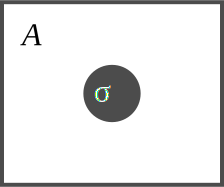
\includegraphics{sigma}
  \caption{Cross section probability}
  \label{fig:sigma}
\end{figure}
Assuming that an interaction will occur (with 100\% probability) if the projectile hits the solid, and not at all (0\% probability) if it misses, the total interaction probability for the single projectile will be
\begin{align}
  \label{eq:pssigma}
  P_S=\frac{\sigma}{A}\,.
\end{align}
Now suppose we have a parallel beam with density of particles $n$ and velocity $v$ towards the target. In time $t$, this beam fills a volume 
\begin{align}
  V=A v t\,.
\end{align}
Choosing $t$ such that the volume contains just one particle, we can write
\begin{align}
  n=1/V\,,
\end{align}
or
\begin{align}
  1=n v t A\,.
\end{align}
replacing back in \eqref{eq:pssigma} we have
\begin{align}
\sigma=\frac{P_s}{n v t}\,.  
\end{align}
$P_s$ is just the decay probability in eq.~\eqref{eq:w2}. Therefore
\begin{align}
  \sigma=\frac{\omega_2}{n v T}=&
\frac{1}{n v T}\int\ldots\int 
(2\pi)^4\delta^{(4)}\left(p_1+p_2-\sum_i k_j\right)VT 
\left|\mathcal{M}_{fi}\right|^2
\frac{1}{2E_{\mathbf{p}_1}V}\frac{1}{2E_{\mathbf{p}_2}V}
\prod_{j=1}^n\frac{d^3k_j}{(2\pi)^32E_{\mathbf{k}_j}}
\nonumber\\
=&\frac{1}{n v V}\int\ldots\int 
(2\pi)^4\delta^{(4)}\left(p_1+p_2-\sum_i k_j\right)
\left|\mathcal{M}_{fi}\right|^2
\frac{1}{2E_{\mathbf{p}_1}}\frac{1}{2E_{\mathbf{p}_2}}
\prod_{j=1}^n\frac{d^3k_j}{(2\pi)^32E_{\mathbf{k}_j}}\,.
\end{align}
The density of particles of the incident state is normalized to one particle  in the entire volume, so that $n=1/V$. Therefore
\begin{align}
   \sigma=&\frac{1}{v}\int\ldots\int 
(2\pi)^4\delta^{(4)}\left(p_1+p_2-\sum_i k_j\right)
\left|\mathcal{M}_{fi}\right|^2
\frac{1}{2E_{\mathbf{p}_1}}\frac{1}{2E_{\mathbf{p}_2}}
\prod_{j=1}^n\frac{d^3k_j}{(2\pi)^32E_{\mathbf{k}_j}}\,.
\end{align}
In general, as both particles may be moving we could use the relative velocity between them, $v_{\text{rel}}$,
\begin{align}
   \sigma=&\frac{1}{v_{\text{rel}}}\int\ldots\int 
(2\pi)^4\delta^{(4)}\left(p_1+p_2-\sum_i k_j\right)
\left|\mathcal{M}_{fi}\right|^2
\frac{1}{2E_{\mathbf{p}_1}}\frac{1}{2E_{\mathbf{p}_2}}
\prod_{j=1}^n\frac{d^3k_j}{(2\pi)^32E_{\mathbf{k}_j}}\,.
\end{align}
In a frame where $\mathbf{p}_1$ and $\mathbf{p}_2$ are along the same line, this reduces to
\begin{align}
  v_{\text{rel}}=\left|
    \frac{\mathbf{p}_1}{E_1}-\frac{\mathbf{p}_2}{E_2}
  \right|\,.
\end{align}
In fact, for not relativistic particles, where $E_i=m_i$, this coincides with the usual relative velocity
\begin{align}
   v_{\text{rel}}=&\left|
    \frac{m_1\mathbf{v}_1}{E_1}-\frac{m_2\mathbf{v}_2}{E_2}
  \right|\nonumber\\
=&\left|
    \mathbf{v}_1-\mathbf{v}_2
  \right|\,.
\end{align}
The most general formula for the relative velocity is 
\begin{align}
  v_{\text{rel}}=\frac{I}{E_1E_2}
\end{align}
where
\begin{align}
  I=&\sqrt{(p_1\cdot p_2)^2-m_1^2m_2^2}  
\end{align}

In general
\begin{align}
  I=&\sqrt{(E_1 E_2-\mathbf{p}_1\cdot\mathbf{p}_2)^2-m_1^2m_2^2}\nonumber\\
  =&\sqrt{E_1^2E_2^2+(\mathbf{p}_1\cdot\mathbf{p}_2)^2-2E_1 E_2\mathbf{p}_1.\mathbf{p}_2 -m_1^2m_2^2}
\end{align}

Since
\begin{align}
  m_1^2m_2^2=&(E_1^2-\mathbf{p}_1^2)(E_2^2-\mathbf{p}_2^2)\nonumber\\
=&(E_1^2E_2^2-\mathbf{p}_1^2E_2^2-E_1^2\mathbf{p}_2^2+\mathbf{p}_1^2\mathbf{p}_2^2)
\end{align}
\begin{align}
  I=\sqrt{\mathbf{p}_1^2E_2^2-2E_1 E_2\mathbf{p}_1\cdot\mathbf{p}_2+E_1^2\mathbf{p}_2^2
+(\mathbf{p}_1\cdot\mathbf{p}_2)^2-
\mathbf{p}_1^2\mathbf{p}_2^2}
\end{align}
If
\begin{align}
  (\mathbf{p}_1\cdot\mathbf{p}_2)^2-
\mathbf{p}_1^2\mathbf{p}_2^2=0
\end{align}
that implies that $\mathbf{p}_1$ and $\mathbf{p}_2$ are colineals,
\begin{align}
  I=&\sqrt{\mathbf{p}_1^2E_2^2-2E_1 E_2\mathbf{p}_1\cdot\mathbf{p}_2+E_1^2\mathbf{p}_2^2}
  \nonumber\\
  =&\sqrt{(\mathbf{p}_1E_2-\mathbf{p}_2E_1)^2}\nonumber\\
  =&|\mathbf{p}_1E_2-\mathbf{p}_2E_1|
\end{align}
\begin{align}
\label{eq:53}
v_{\text{rel}}=  \frac{I}{E_1E_2}=\left|
    \frac{\mathbf{p}_1}{E_1}-\frac{\mathbf{p}_2}{E_2}
  \right|
\end{align}


\begin{borrar}
Consider the collission of a cloud of particles of density $n_1^0$ moving to the right with velocity $v_1^0$ toward another cloud of particles in rest of density $n_2^0$. The differential of number of collisions is
\begin{align}
  d N\propto&|\mathbf{v}_1^0| n_1^0 n_2^0 \,d V\, dt\nonumber\\
  =&\sigma|\mathbf{v}_1^0| n_1^0 n_2^0 \,d V\, dt
\end{align}
Hence,  $\sigma$ have units of area, and corresponds to the cross section. 

The Lorentz invariant expression for velocities and particle densities is
\begin{align}
  |\mathbf{v}_1|^0 n_1^0 n_2^0\to n_1 n_2 \sqrt{(\mathbf{v}_1-\mathbf{v}_2)^2-(\mathbf{v}_1\times\mathbf{v}_2)^2}
\end{align}
Therefore
\begin{align}
  d N =&\sigma\sqrt{(\mathbf{v}_1-\mathbf{v}_2)^2-(\mathbf{v}_1\times\mathbf{v}_2)^2}n_1 n_2 \,d V\, dt  \nonumber\\
  =&\sigma\sqrt{(\mathbf{v}_1-\mathbf{v}_2)^2-(\mathbf{v}_1\times\mathbf{v}_2)^2}\frac{1}{V}(n_1V)(n_2 \,d V)\, dt\nonumber\\
 =&\sigma\sqrt{(\mathbf{v}_1-\mathbf{v}_2)^2-(\mathbf{v}_1\times\mathbf{v}_2)^2}\frac{1}{V}N_1(n_2 \,d V)\, dt\,.
\end{align}
Integrate it out
\begin{align}
  N=&\sigma\sqrt{(\mathbf{v}_1-\mathbf{v}_2)^2-(\mathbf{v}_1\times\mathbf{v}_2)^2}\frac{1}{V}N_1N_2 T
\end{align}
The probability for the collision to happens is
\begin{align}
  \label{eq:52}
  \frac{N}{N_1 N_2}=\frac{\sigma T}{V}\sqrt{(\mathbf{v}_1-\mathbf{v}_2)^2-(\mathbf{v}_1\times\mathbf{v}_2)^2}
\end{align}
The collision probability is according eq.~\eqref{eq:147}
\begin{align}
   \frac{N}{N_1 N_2}
=&\int\ldots\int 
(2\pi)^4\delta^{(4)}\left(p-\sum_i k_j\right)VT 
\left|\mathcal{M}_{fi}\right|^2
\frac{1}{2E_{\mathbf{p}_1}V}\frac{1}{2E_{\mathbf{p}_2}V}
\prod_{j=1}^n\frac{d^3k_j}{(2\pi)^32E_{\mathbf{k}_j}}
\end{align}
Replacing back in eq.~\eqref{eq:52}, we have that the  cross section is
\begin{align}
  \sigma=&\frac{V}{T\sqrt{(\mathbf{v}_1-\mathbf{v}_2)^2-(\mathbf{v}_1\times\mathbf{v}_2)^2}}\nonumber\\
&\times\int\ldots\int 
(2\pi)^4\delta^{(4)}\left(p_1+p_2-\sum_i k_j\right)VT 
\left|\mathcal{M}_{fi}\right|^2
\frac{1}{2E_{\mathbf{p}_1}V}\frac{1}{2E_{\mathbf{p}_2}V}
\prod_{j=1}^n\frac{d^3k_j}{(2\pi)^32E_{\mathbf{k}_j}}
\end{align}
Defining
\begin{align}
  I=E_{\mathbf{p}_1} E_{\mathbf{p}_2} \sqrt{(\mathbf{v}_1-\mathbf{v}_2)^2-(\mathbf{v}_1\times\mathbf{v}_2)^2}
\end{align}
we have the differential cross section as
\begin{align}
  d\sigma=&\frac{V E_{\mathbf{p}_1} E_{\mathbf{p}_2} }{T I}
(2\pi)^4\delta^{(4)}\left(p_1+p_2-\sum_i k_j\right)VT 
\left|\mathcal{M}_{fi}\right|^2
\frac{1}{2E_{\mathbf{p}_1}V}\frac{1}{2E_{\mathbf{p}_2}V}
\prod_{j=1}^n\frac{d^3k_j}{(2\pi)^32E_{\mathbf{k}_j}}
\end{align}
In this way, when the initial state in the $S$--matrix contains two particles
\begin{align}
  d\sigma=(2\pi)^4\delta^{(4)}\left(\sum_{i=1,2} p_i-\sum_{j}k_j\right)
\frac{1}{4I}\left|\mathcal{M}_{fi}\right|^2
\prod_{j}\frac{d^3k_j}{(2\pi)^32E_{\mathbf{k}_j}}
\end{align}
where
\begin{align}
  I=&\sqrt{(p_1\cdot p_2)^2-m_1^2m_2^2}\nonumber\\
=&E_{\mathbf{p}_1} E_{\mathbf{p}_2} \sqrt{(\mathbf{v}_1-\mathbf{v}_2)^2-(\mathbf{v}_1\times\mathbf{v}_2)^2}
\end{align}
Defining 
\begin{align}
  v_{\text{rel}}=\frac{I}{E_1E_2}
\end{align}
In general
\begin{align}
  I=&\sqrt{(E_1 E_2-\mathbf{p}_1\cdot\mathbf{p}_2)^2-m_1^2m_2^2}\nonumber\\
  =&\sqrt{E_1^2E_2^2+(\mathbf{p}_1\cdot\mathbf{p}_2)^2-2E_1 E_2\mathbf{p}_1.\mathbf{p}_2 -m_1^2m_2^2}
\end{align}

Since
\begin{align}
  m_1^2m_2^2=&(E_1^2-\mathbf{p}_1^2)(E_2^2-\mathbf{p}_2^2)\nonumber\\
=&(E_1^2E_2^2-\mathbf{p}_1^2E_2^2-E_1^2\mathbf{p}_2^2+\mathbf{p}_1^2\mathbf{p}_2^2)
\end{align}
\begin{align}
  I=\sqrt{\mathbf{p}_1^2E_2^2-2E_1 E_2\mathbf{p}_1\cdot\mathbf{p}_2+E_1^2\mathbf{p}_2^2
+(\mathbf{p}_1\cdot\mathbf{p}_2)^2-
\mathbf{p}_1^2\mathbf{p}_2^2}
\end{align}
If
\begin{align}
  (\mathbf{p}_1\cdot\mathbf{p}_2)^2-
\mathbf{p}_1^2\mathbf{p}_2^2=0
\end{align}
that implies that $\mathbf{p}_1$ and $\mathbf{p}_2$ are colineals,
\begin{align}
  I=&\sqrt{\mathbf{p}_1^2E_2^2-2E_1 E_2\mathbf{p}_1\cdot\mathbf{p}_2+E_1^2\mathbf{p}_2^2}
  \nonumber\\
  =&\sqrt{(\mathbf{p}_1E_2-\mathbf{p}_2E_1)^2}\nonumber\\
  =&|\mathbf{p}_1E_2-\mathbf{p}_2E_1|
\end{align}
\begin{align}
\label{eq:53}
v_{\text{rel}}=  \frac{I}{E_1E_2}=\left|
    \frac{\mathbf{p}_1}{E_1}-\frac{\mathbf{p}_2}{E_2}
  \right|
\end{align}
\end{borrar}
To simplify the notation we set $E_i=E_{\mathbf{p}_i}=$, and $E_f=E_{\mathbf{p}_f}$. Moreover, the differential cross section is
\begin{align}
    d\sigma=&(2\pi)^4\delta^{(4)}\left(\sum_{i=1}^2p_i-\sum_{f} p_f\right)
\frac{1}{4v_{\text{rel}}E_1E_2}\left|\mathcal{M}_{fi}\right|^2
\prod_{f}\frac{d^3k_f}{(2\pi)^32E_{f}}\nonumber\\
&=(2\pi)^4\frac{1}{4v_{\text{rel}}E_1E_2}\left|\mathcal{M}_{fi}\right|^2
d\Phi^{n}(p_1,p_2;k_1,\ldots,k_n)
\end{align}
where
\begin{align}
  \label{eq:50}
    d \Phi^{(n)} (p_1,p_2; k_1, k_2,\dots, k_n) = \delta^{(4)}\left(p-\sum_j k_j\right)  \prod_{j=1}^n \frac{d^3 k_j}{(2\pi)^3 2 E_{\mathbf{k}_j}} \,.
\end{align}
We keep the diferential notation both for $d\sigma$, and $d\Phi$ until the last integration have been made.

\subsection{2--to--2 cross section}
\label{sec:2-2-cross}

The the 2--to--2 cross section is
\begin{align}
 \label{eq:54}
  d\sigma=&\frac{(2\pi)^4}{4v_{\text{rel}}E_1E_2}\left|\mathcal{M}_{fi}\right|^2
d\Phi^{2}(p_1,p_2;p'_1,p'_2)\nonumber\\
=&\frac{2^4\pi^4}{2^{8}\pi^64v_{\text{rel}}E_1E_2}2^{8}\pi^6\left|\mathcal{M}_{fi}\right|^2
d\Phi^{n}(p_1,p_2;k_1,\ldots,k_n)\nonumber\\
=&\frac{1}{2^{6}\pi^2v_{\text{rel}}E_1E_2}\left|\mathcal{M}_{fi}\right|^2
\left[4(2\pi)^6d\Phi^{2}(p_1,p_2;p'_1,p'_2)\right]\nonumber\\
=&\frac{1}{64\pi^2v_{\text{rel}}E_1E_2}\left|\mathcal{M}_{fi}\right|^2
\left[4(2\pi)^6d\Phi^{2}(p_1,p_2;p'_1,p'_2)\right]
\end{align}
where, as in eq.~\eqref{eq:50}
\begin{align}
4(4\pi)^6d\Phi^{(2)}(p_1,p_2;p_1',p_2')&= \frac{4(4\pi)^6}{4(2\pi)^6} \delta^{(4)}\left(p_1+p_2-p_1'-p_2'\right)
\frac{d^3p_1'}{E_{1}'}\frac{d^3p_2'}{E_{2}'}\nonumber\\
&=  \delta^{(4)}\left(p_1+p_2-p_1'-p_2'\right)4(2\pi)^6
\frac{d^3p_1'}{E_{1}'}\frac{d^3p_2'}{E_{2}'}
\end{align}
We now will find an expression for cross section in the center of mass frame (CM) 


The center of mass (CM) frame is defined by the condition
\begin{align}
  \label{eq:cm}
  \mathbf{p}_1+\mathbf{p}_2=0
\end{align}


The $\delta$--function in Eq.~\eqref{eq:101}
\begin{align}
\label{eq:56}
  \delta^{(4)}(p+p_2-p_1'-p_2')=\delta^{(3)}(\mathbf{p}_1+\mathbf{p}_2-\mathbf{p}_1'-\mathbf{p}_2')
\delta(E_1+E_2-E_1'-E_2')
\end{align}
In the CM frame
\begin{align}
\label{eq:148}
  \delta^{(4)}(p+p_2-p_1'-p_2')=\delta^{(3)}(\mathbf{p}_1'+\mathbf{p}_2')
\delta(E_1+E_2-E_1'-E_2')
\end{align}
$\mathcal{M}_{fi}$ in integration does not depend on $|\mathbf{p}_1'|$ or $|\mathbf{p}_2'|$ as the final momentum is fixed by the initial momentum whenever the final states have only two particles. In this way the integration on $p_2'$ can be evaluated directly for $d\Phi^{(2)}$. Replacing back in Eq.~\eqref{eq:54}
\begin{align}
\label{eq:149}
  4(2\pi)^6d\Phi^{(2)}=&\delta^{(3)}(\mathbf{p}_1'+\mathbf{p}_2')\delta(E_1+E_2-E_1'-E_2')
\frac{d^3p_1'}{E_{1}'}\frac{d^3p_2'}{E_{2}'}\nonumber\\
 =&\delta(E_1+E_2-E_1'-E_2')
\frac{d^3p_1'}{E_{1}'}\int\delta^{(3)}(\mathbf{p}_1'+\mathbf{p}_2')\frac{d^3p_2'}{E_{2}'}\nonumber\\
=&\delta(E_1+E_2-E_1'-E_2')
\frac{d^3p_1'}{E_{1}'E_{2}'}
\end{align}

\begin{align}
  4(2\pi)^6d\Phi^{(2)}=\delta(E_1+E_2-E_1'-E_2')
  \frac{{\mathbf{p}_1'}^2d|\mathbf{p}_1'|d\Omega}{E_{1}'E_{2}'}
\end{align}

As
\begin{align}
  |\mathbf{p}_1'|=\sqrt{{E_1'}^2-{m_1}^2}
\end{align}

\begin{align}
  \frac{d|\mathbf{p}_1'|}{dE_1'}=&\frac{2E_1'}{2\sqrt{{E_1'}^2-{m_1}^2}}\nonumber\\
  =&\frac{E_1'}{|\mathbf{p}_1'|}
\end{align}
In this way, we can write, in general
\begin{align}
 |\mathbf{p}|\, d|\mathbf{p}|=E\,dE
\end{align}
and
\begin{align}
\label{eq:57}
 4(2\pi)^6 d\Phi^{(2)}&=\delta(E_1+E_2-E_1'-E_2')
\frac{|\mathbf{p}_1'|E_1'dE_1'}{E_{1}'E_{2}'}d\Omega\nonumber\\
  &=\delta(E_1+E_2-E_1'-E_2')
\frac{|\mathbf{p}_1'|dE_1'}{E_{2}'}d\Omega
\end{align}
From the $\delta$--function in Eq.~\eqref{eq:56} we have that in the CM frame
\begin{align}
  \mathbf{p}_1+\mathbf{p}_2-\mathbf{p}_1'-\mathbf{p}_2'=0 \overset{\text{CM}}{\Rightarrow}
  \begin{cases}
    \mathbf{p}_1=-\mathbf{p}_2\\
    \mathbf{p}_1'=-\mathbf{p}_2'\\
  \end{cases}
\end{align}

Squaring the first expression, and taking into account that
\begin{align}
  \label{eq:58}
  {\mathbf{p}'_1}= \sqrt{{E_1'}^2-{m_1'}^2}
\end{align}
we have
\begin{align}
  {\mathbf{p}'_1}^2=&{\mathbf{p}'_2}^2\nonumber\\
  {E_1'}^2-{m_1'}^2=&  {E_2'}^2-{m_2'}^2\,,
\end{align}
\begin{align}
\label{eq:59}
  E_2'=\sqrt{{E_1'}^2-{m_1'}^2+{m_2'}^2}
\end{align}
In this way we can express $E_2'$ in terms of $E_1'$ in Eq.~\eqref{eq:57}.
Moreover, we can define the center of mass energy as
\begin{align}
\label{eq:smv}
  s=&\left( p_1+p_2 \right)^2\,.
\end{align}

By using the center of mass condition \eqref{eq:cm}
\begin{align}
  \mathbf{p}=\mathbf{p}_1=-\mathbf{p}_2\,,
\end{align}
then
\begin{align}
   s=& p_1^2+p_2^2+2 p_1\cdot p_2 \nonumber\\
=&  p_1^2+p_2^2+2  \left( E_1 E_2-\mathbf{p}_1\cdot\mathbf{p}_2 \right)\nonumber\\
=& p_1^2+p_2^2+2\left( E_1 E_2+\mathbf{p}_1^2 \right) \nonumber\\
=& p_1^2+p_2^2+2\left( E_1 E_2+ E_1^2-p_1^2 \right) \nonumber\\
=& p_1^2+p_2^2+2\left( E_1 E_2+ E_1^2-p_1^2 \right) \nonumber\\
=& p_2^2-p_1^2+2\left( E_1 E_2+ E_1^2 \right) \nonumber\\
=& E_2^2-\mathbf{p}_1^2-E_2^2+\mathbf{p}_2^2+2\left( E_1 E_2+ E_1^2 \right) \nonumber\\
=& E_2^2-E_1^2+2\left( E_1 E_2+ E_1^2 \right) \nonumber\\
=& E_1^2 +2E_1 E_2+ E_2^2 \nonumber\\
=& \left( E_1+E_2 \right)^2\,.
\end{align}
So that
\begin{align}
  \label{eq:60}
  \sqrt{s}=E_1+E_2
\end{align}
Using The energy part of $\delta$--function in Eq.~\eqref{eq:56} can be written as
\begin{align}
  \delta\left(\sqrt{s}-E_1'-\sqrt{{E_1'}^2-{m_1'}^2+{m_2'}^2}\right)
\end{align}
As established before,  $\mathcal{M}_{fi}$ in this case in independent of $|\mathbf{p}'_1|$, and the integration on $E_1'$ can be done directly only for $d\Phi^{(2)}$.
The integral is easily performed using the identity
\begin{align}
  \delta\left(f(z)\right)=\sum_n\frac{\delta(z-z_n)}{|f'(z_n)|}
\end{align}
where $z_n$ are the zeroes of $f(z)$. In this case, this $\delta$--function is a function of the integration variable $E_1'$, with only one zero
\begin{align}
   \delta\left(f(x)\right)=\frac{\delta(x-x_0)}{|f'(x_0)|}
\end{align}
where
\begin{align}
  f(x)=\sqrt{s}-x-\sqrt{x^2-{m_1'}^2+{m_2'}^2}
\end{align}
Therefore
\begin{align}
  \label{eq:61}
   4(2\pi)^6d\Phi^{(2)}=&d\Omega\int\frac{\delta(x-x_0)}{|f'(x_0)|}\frac{
     |\mathbf{p}_1'(x)|}{E_2'(x)}dx\nonumber\\
   =&d\Omega\frac{1}{|f'(x_0)|}\frac{
     |\mathbf{p}_1'(x_0)|}{E_2'(x_0)}\nonumber\\
\end{align}
where from Eqs.~\eqref{eq:58}, \eqref{eq:59},
\begin{align}
  \label{eq:62}
  \mathbf{p}_1'(x_0)=&\sqrt{x_0^2-{m_1'}^2}&
  E_2'(x_0)=&\sqrt{x_0^2-{m_1'}^2+{m_2'}^2}
\end{align}
The zero is obtained from
\begin{align}
  &\sqrt{s}-x_0-\sqrt{x_0^2-{m_1'}^2+{m_2'}^2}=0\nonumber\\
  &s-2\sqrt{s}\,x_0+x_0^2=x_0^2-{m_1'}^2+{m_2'}^2\nonumber\\
  &s-2\sqrt{s}\,x_0=-{m_1'}^2+{m_2'}^2
\end{align}
with solution
\begin{align}
  \label{eq:63}
  x_0=\frac{s+{m_1'}^2-{m_2'}^2}{2\sqrt{s}}
\end{align}
As (See 
\texttt{deltaxn.nb} %noinstiki [deltax.nb](Appendix)
for additional details)
\begin{align}
  f'(x)=-\frac{x}{\sqrt{x^2-{m_1'}^2+{m_2'}^2}}-1
\end{align}
we have
\begin{align}
  \label{eq:64}
  f'(x_0)=&-\frac{{m_1'}^2-{m_2'}^2+s}{\sqrt{s}
   \sqrt{\frac{\left(-{m_1'}^2+{m_2'}^2+s\right)^2}{s}}}-1\nonumber\\
    =&\frac{-{m_1'}^2+{m_2'}^2-s}{-{m_1'}^2+{m_2'}^2+s}-1\nonumber\\
    =&\frac{-{m_1'}^2+{m_2'}^2-s+{m_1'}^2-{m_2'}^2-s}{-{m_1'}^2+{m_2'}^2+s}\nonumber\\
=&\frac{-2s}{s+{m_2'}^2-{m_1'}^2}\,,
\end{align}
and
\begin{align}
  \label{eq:65}
  \delta(f(E_1'))=\delta(E_1'-x_0)\left(\frac{s+{m_2'}^2-{m_1'}^2}{2s}\right)
\end{align}

Replacing the expression for $x_0$ in \eqref{eq:63} into Eq.~\eqref{eq:62} we have (See 
\texttt{deltaxn.nb}  %noinstiki [deltax.nb](Appendix)
for additional details)
\begin{align}
  \label{eq:66}
   |\mathbf{p}_1'(x_0)|=&\frac{\sqrt{[s-({m_1'}-{m_2'})^2][s-({m_1'}+{m_2'})^2]}}{2\sqrt{s}}\nonumber\\
E_2'(x_0)=&  \frac{s-{m_1'}^2+{m_2'}^2}{2\sqrt{s}}
\end{align}

Replacing Eqs.~\eqref{eq:64}, and \eqref{eq:66} in Eq.~\eqref{eq:61}
we have
\begin{align}
  \label{eq:67}
4(2\pi)^6d\Phi^{(2)}&=d\Omega\frac{1}{|f'(x_0)|}
\frac{\sqrt{x_0^2-{m_1'}^2}}{\sqrt{x_0^2-{m_1'}^2+{m_2'}^2}}\nonumber\\
  &=d\Omega\left(\frac{s-{m_1'}^2+{m_2'}^2}{2s}\right)
\frac{\sqrt{[s-({m_1'}-{m_2'})^2][s-({m_1'}+{m_2'})^2]}}{s-{m_1'}^2+{m_2'}^2}\nonumber\\
&=d\Omega\frac{\sqrt{[s-({m_1'}-{m_2'})^2][s-({m_1'}+{m_2'})^2]}}{2s}
\end{align}
Defining the kinematic two particle function
\begin{align}
  \label{eq:46}
  \lambda(a,b,c)\equiv(a-b+c)^2-4ac
\end{align}
and taking into account that
\begin{align}
  \left(s-{m_2'}^2+{m_1'}^2\right)^2-4s{m_1'}^2=[s-({m_1'}-{m_2'})^2][s-({m_1'}+{m_2'})^2]
\end{align}
we have
\begin{align}
\label{eq:150}
  4(2\pi)^6d\Phi^{(2)}=d\Omega\frac{\lambda^{1/2}(s,{m_2'}^2,{m_1'}^2)}{2s}
\end{align}
Moreover
\begin{align}
  \label{eq:151}
  \mathbf{p}_1'=&\frac{\lambda^{1/2}(s,{m_2'}^2,{m_1'}^2)}{2\sqrt{s}}
\end{align}
%\left(\right)

To further evaluate Eq.~(\ref{eq:54}), we need to express $v_{\text{rel}}$ and $E_1E_2$ in terms of $s$ and the masses. Concerning $v_{\text{rel}}$,
from Eq.~\eqref{eq:53}, evaluated in CM frame
\begin{align}
  \label{eq:68}
    E_1E_2 v_{\text{rel}}=&E_1E_2\left|\frac{\mathbf{p}_1}{E_1}-\frac{\mathbf{p}_2}{E_2}\right|\nonumber\\
  =&E_1E_2\left|\frac{\mathbf{p}_1}{E_1}+\frac{\mathbf{p}_1}{E_2}\right|\nonumber\\
  =&\left|\mathbf{p}_1\right|({E_1+E_2})\nonumber\\
  =&\left|\mathbf{p}_1\right|\sqrt{s}
\end{align}
Replacing back Eqs.~\eqref{eq:67}, and \eqref{eq:68} into Eq.~\eqref{eq:54}, we have
\begin{align}
  \label{eq:69}
      d\sigma=&\frac{1}{64\pi^2E_1E_2v_{\text{rel}}}\overline{\left|\mathcal{M}_{fi}\right|^2}
    \left[4(2\pi)^6d\Phi^{(2)}\right]
\end{align}
\begin{align}
  \frac{d\sigma}{d\Omega}=\frac{1}{64\pi^2E_1E_2v_{\text{rel}}}\overline{\left|\mathcal{M}_{fi}\right|^2}
\frac{\sqrt{[s-({m_1'}+{m_2'})^2][s-({m_1'}-{m_2'})^2]}}{2s}
\end{align}
By using Eq.~\eqref{eq:68}
\begin{align}
  \frac{d\sigma}{d\Omega}=\frac{1}{64\pi^2|\mathbf{p}_1|\sqrt{s}}\overline{\left|\mathcal{M}_{fi}\right|^2}
\frac{\sqrt{[s-({m_1'}+{m_2'})][s-({m_1'}^2-{m_2'}^2)]}}{2s}
\end{align}
In the CM frame
\begin{align}
\sqrt{s}=&E_1+E_2\nonumber\\
=&\sqrt{\mathbf{p}_1^2+m_1^2}+\sqrt{\mathbf{p}_2^2+m_2^2}\nonumber\\
=&\sqrt{\mathbf{p}_1^2+m_1^2}+\sqrt{\mathbf{p}_1^2+m_2^2}
\end{align}

\begin{align}
  \label{eq:70}
  s=&2\mathbf{p}_1^2+m_1^2+m_2^2+2\sqrt{\mathbf{p}_1^4+(m_1^2+m_2^2)\mathbf{p}_1^2+m_1^2m_2^2}\nonumber\\
s-(2\mathbf{p}_1^2+m_1^2+m_2^2)=&2\sqrt{\mathbf{p}_1^4+(m_1^2+m_2^2)\mathbf{p}_1^2+m_1^2m_2^2}
\end{align}
\begin{align}
  s^2-2s(2\mathbf{p}_1^2+m_1^2+m_2^2)+[2\mathbf{p}_1^2+(m_1^2+m_2^2)]^2=&4(\mathbf{p}_1^4+(m_1^2+m_2^2)\mathbf{p}_1^2+m_1^2m_2^2)\nonumber\\
  s^2-2s(2\mathbf{p}_1^2+m_1^2+m_2^2)+4\mathbf{p}_1^4+4\mathbf{p}_1^2(m_1^2+m_2^2)
+(m_1^2+m_2^2)^2=&4(\mathbf{p}_1^4+(m_1^2+m_2^2)\mathbf{p}_1^2+m_1^2m_2^2)\nonumber\\
-4s\mathbf{p}_1^2+s^2-2s(m_1^2+m_2^2)+(m_1^2+m_2^2)^2=&4m_1^2m_2^2\nonumber\\
-4s\mathbf{p}_1^2+s^2-2sm_1^2-2sm_2^2+m_1^4+m_2^4+2m_1^2m_2^2=&4m_1^2m_2^2\nonumber\\
-4s\mathbf{p}_1^2+s^2-2sm_1^2-2sm_2^2+m_1^4+m_2^4-2m_1^2m_2^2=&0
\end{align}
\begin{align}
  \mathbf{p}_1^2=\frac{\left(s-m_1^2-2 m_2 m_1-m_2^2\right)
   \left(s-m_1^2+2 m_2m_1-m_2^2\right)}
{4s}
\end{align}
\begin{align}
  \label{eq:71}
  |\mathbf{p}_1|=&\frac{\sqrt{[s-(m_1+m_2)^2][s-(m_1-m_2)^2]}}{2\sqrt{s}}\nonumber\\
=&\frac{\lambda^{1/2}(s,m_2^2,m_1^2)}{2\sqrt{s}}
\end{align}
Replacing Eq.~\eqref{eq:71} back in Eq.~\eqref{eq:68} we have
\begin{align}
  \label{eq:72}
  E_1E_2 v_{\text{rel}}=\frac{1}{2}\sqrt{[s-(m_1+m_2)^2][s-(m_1-m_2)^2]}
\end{align}
Replacing Eqs.~\eqref{eq:72}, and \eqref{eq:67} in Eq.~\eqref{eq:54}
\begin{align}
  \label{eq:73}
  d\sigma=&\frac{1}{64\pi^2}\overline{\left|\mathcal{M}_{fi}\right|^2}\frac{d\Omega}{2s}(2)
\sqrt{\frac{[s-(m_1'+m_2')^2][s-(m_1'-m_2')^2]}{[s-(m_1+m_2)^2][s-(m_1-m_2)^2]}}
\end{align}
and, finally
\begin{align}
  \frac{d\sigma}{d\Omega}=\frac{1}{64\pi^2s}\left\{
\frac{[s-(m_1'+m_2')^2][s-(m_1'-m_2')^2]}{[s-(m_1+m_2)^2][s-(m_1-m_2)^2]}\right\}^{1/2}
\overline{|\mathcal{M}|^2}
\end{align}
or, in terms of the kinematic function defined in eq.~\eqref{eq:46}
\begin{align}
  \label{eq:2bcs}
  \frac{d\sigma}{d\Omega}=\frac{1}{64\pi^2s}
\frac{\lambda^{1/2}(s,{m_2'}^2,{m_1'}^2)}{\lambda^{1/2}(s,m_2^2,m_1^2)}
\overline{|\mathcal{M}|^2}
\end{align}
%\left(\right)

\section{Decay Rates}
\label{sec:decay-rates}
Consider the matrix element of $i T$ in (\ref{eq:41})
\begin{align}
  \label{eq:45}
  \langle\mathbf{k}_1\ldots\mathbf{k}_n|i T|\mathbf{p}\rangle^{\text{NR}}=(2\pi)^4\delta^{(4)}\left(p-\sum_i k_i\right)i{M}_{fi}
\end{align}

where the initial state is a single particle of momentum $p$ and mass $M$, while the final state is given by $n$ particles of momenta $k_i$ and masses $m_i$, $i=1,\ldots,n$. 
We are therefore considering a decay process. 


By using eq.~\eqref{eq:146} we have
\begin{align}
\omega=&\int\ldots\int 
(2\pi)^4\delta^{(4)}\left(p-\sum_i k_j\right)\left(\int dt\right) 
\left|\mathcal{M}_{fi}\right|^2
\frac{1}{2E_{\mathbf{p}}}
\prod_{j=1}^n\frac{d^3k_j}{(2\pi)^32E_{\mathbf{k}_j}}
\end{align}
Therefore the differential probability is
\begin{align}
  d\omega=&
(2\pi)^4\delta^{(4)}\left(p-\sum_i k_j\right)
\frac{1}{2E_{\mathbf{p}}}\left|\mathcal{M}_{fi}\right|^2
dt\prod_{j=1}^n\frac{d^3k_j}{(2\pi)^32E_{\mathbf{k}_j}}
\end{align}
Finally we define the \textit{decay rate} $d\Gamma$ as the decay probability in which in the final state
the j--th particle has momentum between $k_j$ and $k_j+ dk_j$ per unit time
\begin{align}
\label{eq:49}
d\Gamma\equiv&\frac{d\omega}{dt}=
(2\pi)^4\delta^{(4)}\left(p-\sum_j k_j\right)
\frac{1}{2E_{\mathbf{p}}}\left|\mathcal{M}_{fi}\right|^2
\prod_{j=1}^n\frac{d^3k_j}{(2\pi)^32E_{\mathbf{k}_j}}\nonumber\\
=&\frac{(2\pi)^4}{2E_{\mathbf{p}}}\left|\mathcal{M}_{fi}\right|^2
d \Phi^{(n)} (p; k_1, k_2,\dots, k_n)
\end{align}
where
\begin{align}
  \label{eq:50}
    d \Phi^{(n)} (p; k_1, k_2,\dots, k_n) = \delta^{(4)}\left(p-\sum_j k_j\right)  \prod_{j=1}^n \frac{d^3 k_j}{(2\pi)^3 2 E_{\mathbf{k}_j}} \,.
\end{align}
and the differential decay width in the center of mass frame
\begin{align}
  \label{eq:51}
  d\Gamma=\frac{(2\pi)^4}{2E_{\mathbf{p}}}\left|\mathcal{M}_{fi}\right|^2
d \Phi^{(n)} (p; k_1, k_2,\dots, k_n)
\end{align}


\subsection{Two body decays}
We now consider the decay of particle of mass $M$ decaying into two particles of 4--momenta $p_1$, $p_2$ and masses $m_1$, $m_2$. In the CM frame the initial momentum satisfy
\begin{align}
  \mathbf{p}=&0\Rightarrow M=E_{\mathbf{p}}
\end{align}
Therefore 
\begin{align}
  \label{eq:51nn}
  d\Gamma=&\frac{(2\pi)^4}{2M[4(2\pi)^6]}\left|\mathcal{M}_{fi}\right|^2
4(2\pi)^6d \Phi^{(2)} (p; p_1, p_2)\nonumber\\
=&\frac{1}{2^3M(2\pi)^2}\left|\mathcal{M}_{fi}\right|^2
4(2\pi)^6d \Phi^{(2)} (p; p_1, p_2)\nonumber\\
=&\frac{1}{32 \pi^2M}\left|\mathcal{M}_{fi}\right|^2
\left[4(2\pi)^6d \Phi^{(2)} (p; p_1, p_2)\right]
\end{align}
where
\begin{align}
  4(2\pi)^6d \Phi^{(2)} (p; p_1, p_2)=\delta^{(4)}(p-p_1-p_2)\frac{d^3p_1}{E_{1}}\frac{d^3p_2}{E_{2}}
\end{align}
The Dirac delta in eq.~\eqref{eq:50} can be written in the CM frame as
\begin{align}
\label{eq:153}
  \delta^{(4)}(p-p_1-p_2)=&\delta^{(3)}(\mathbf{p}-\mathbf{p}_1-\mathbf{p}_2)\delta(E-E_1-E_2)\nonumber\\
=&\delta^{(3)}(\mathbf{p}_1+\mathbf{p}_2)\delta(M-E_1-E_2)
\end{align}
and,
\begin{align}
   4(2\pi)^6d \Phi^{(2)} (p; p_1, p_2)=&\delta(M-E_1-E_2)\delta^{(3)}(\mathbf{p}_1+\mathbf{p}_2)\frac{d^3p_1}{E_{1}}\frac{d^3p_2}{E_{2}}
\end{align}
We now proceed  with a calculation similat to the one leading to eq.~\eqref{eq:149} \footnote{ we see that the two quantities are the same after the replacing $\sqrt{s}\to M$, $p_1'\to p_1$ and $p_2'\to p_2$.} 
\begin{align}
\label{eq:149nn}
  4(2\pi)^6d\Phi^{(2)}=&\delta^{(3)}(\mathbf{p}_1+\mathbf{p}_2)\delta(M-E_1-E_2)
\frac{d^3p_1}{E_{1}}\frac{d^3p_2}{E_{2}}\nonumber\\
 =&\delta(M-E_1-E_2)
\frac{d^3p_1}{E_{1}}\int\delta^{(3)}(\mathbf{p}_1+\mathbf{p}_2)\frac{d^3p_2}{E_{2}}\nonumber\\
=&\delta(M-E_1-E_2)
\frac{d^3p_1}{E_{1}E_{2}}
\end{align}

\begin{align}
  4(2\pi)^6d\Phi^{(2)}=\delta(M-E_1-E_2)
  \frac{{\mathbf{p}_1}^2d|\mathbf{p}_1|d\Omega}{E_{1}E_{2}}
\end{align}

As
\begin{align}
  |\mathbf{p}_1|=\sqrt{{E_1}^2-{m_1}^2}
\end{align}

\begin{align}
  \frac{d|\mathbf{p}_1|}{dE_1}=&\frac{2E_1}{2\sqrt{{E_1}^2-{m_1}^2}}\nonumber\\
  =&\frac{E_1}{|\mathbf{p}_1|}
\end{align}
In this way, we can write, in general
\begin{align}
 |\mathbf{p}|\, d|\mathbf{p}|=E\,dE
\end{align}
and
\begin{align}
 4(2\pi)^6 d\Phi^{(2)}&=\delta(M-E_1-E_2)
\frac{|\mathbf{p}_1|E_1dE_1}{E_{1}E_{2}}d\Omega\nonumber\\
  &=\delta(M-E_1-E_2)
\frac{|\mathbf{p}_1|dE_1}{E_{2}}d\Omega
\end{align}
From the $\delta$--function in Eq.~\eqref{eq:56} we have that in the CM frame
\begin{align}
 \mathbf{p}_1-\mathbf{p}_2=0 \overset{\text{CM}}{\Rightarrow}
    \mathbf{p}_1=-\mathbf{p}_2
\end{align}

Squaring the first expression, and taking into account that
\begin{align}
  {\mathbf{p}_1}= \sqrt{{E_1}^2-{m_1}^2}
\end{align}
we have
\begin{align}
  {\mathbf{p}_1}^2=&{\mathbf{p}_2}^2\nonumber\\
  {E_1}^2-{m_1}^2=&  {E_2}^2-{m_2}^2\,,
\end{align}
\begin{align}
  E_2=\sqrt{{E_1}^2-{m_1}^2+{m_2}^2}
\end{align}
In this way we can express $E_2$ in terms of $E_1$ in Eq.~\eqref{eq:57}.

Using The energy part of $\delta$--function in Eq.~\eqref{eq:56} can be written as
\begin{align}
  \delta\left(M-E_1-\sqrt{{E_1}^2-{m_1}^2+{m_2}^2}\right)
\end{align}
As established before,  $\mathcal{M}_{fi}$ in this case in independent of $|\mathbf{p}_1|$, and the integration on $E_1$ can be done directly only for $d\Phi^{(2)}$.

The integral is easily performed using the identity
\begin{align}
   \delta\left(f(x)\right)=\frac{\delta(x-x_0)}{|f'(x_0)|}
\end{align}
where
\begin{align}
  f(x)=M-x-\sqrt{x^2-{m_1}^2+{m_2}^2}
\end{align}
and the root is given by~\eqref{eq:63}
\begin{align}
  x_0=\frac{M^2+{m_1}^2-{m_2}^2}{2M}
\end{align}

Therefore
\begin{align}
  \label{eq:61nn}
   4(2\pi)^6d\Phi^{(2)}=&d\Omega\int\frac{\delta(x-x_0)}{|f'(x_0)|}\frac{
     |\mathbf{p}_1(x)|}{E_2(x)}dx\nonumber\\
   =&d\Omega\frac{1}{|f'(x_0)|}\frac{
     |\mathbf{p}_1(x_0)|}{E_2(x_0)}\,,
\end{align}
where 
\begin{align}
  \label{eq:62nn}
  \mathbf{p}_1(x_0)=&\sqrt{x_0^2-{m_1}^2}&
  E_2(x_0)=&\sqrt{x_0^2-{m_1}^2+{m_2}^2}
\end{align}

As (See 
\texttt{deltaxn.nb} %noinstiki [deltax.nb](Appendix)
for additional details)
\begin{align}
  f'(x)=-\frac{x}{\sqrt{x^2-{m_1}^2+{m_2}^2}}-1
\end{align}
we have as in~\eqref{eq:64}
\begin{align}
  \label{eq:64nn}
  f'(x_0)=&\frac{-2M^2}{M^2+{m_2}^2-{m_1}^2}\,,
\end{align}
and
\begin{align}
  \label{eq:65nn}
  \delta(f(E_1))=\delta(E_1-x_0)\left(\frac{M^2+{m_2}^2-{m_1}^2}{2M^2}\right)
\end{align}

Replacing the expression for $x_0$ in into Eq.~\eqref{eq:62nn} we have (See 
\texttt{deltaxn.nb}  %noinstiki [deltax.nb](Appendix)
for additional details)
\begin{align}
  \label{eq:66nn}
  |\mathbf{p}_1(x_0)|=&\frac{\sqrt{[M^2-({m_1}-{m_2})^2][M^2-({m_1}+{m_2})^2]}}{2M}\nonumber\\
E_2(x_0)=&  \frac{M^2-{m_1}^2+{m_2}^2}{2M}
\end{align}

Replacing Eqs.~\eqref{eq:64nn}, and \eqref{eq:66nn} in Eq.~\eqref{eq:61nn}
we have
\begin{align}
  \label{eq:67nn}
4(2\pi)^6d\Phi^{(2)}&=d\Omega\frac{1}{|f'(x_0)|}
\frac{\sqrt{x_0^2-{m_1}^2}}{\sqrt{x_0^2-{m_1}^2+{m_2}^2}}\nonumber\\
  &=d\Omega\left(\frac{M^2-{m_1}^2+{m_2}^2}{2M^2}\right)
\frac{\sqrt{[M^2-({m_1}-{m_2})^2][M^2-({m_1}+{m_2})^2]}}{M^2-{m_1}^2+{m_2}^2}\nonumber\\
&=d\Omega\frac{\sqrt{[M^2-({m_1}-{m_2})^2][M^2-({m_1}+{m_2})^2]}}{2M^2}
\end{align}
Defining the kinematic two particle function
\begin{align}
  \label{eq:46}
  \lambda(a,b,c)\equiv(a-b+c)^2-4ac
\end{align}
and taking into account that
\begin{align}
  \left(M^2-{m_2}^2+{m_1}^2\right)^2-4M^2{m_1}^2=[M^2-({m_1}-{m_2})^2][M^2-({m_1}+{m_2})^2]
\end{align}
we have
\begin{align}
\label{eq:150nn}
4(2\pi)^6d\Phi^{(2)}=d\Omega\frac{\lambda^{1/2}(M^2,{m_2}^2,{m_1}^2)}{2M^2}
\end{align}


Finally  we get a similar result than in eq.~\eqref{eq:150}
\begin{align}
    4(2\pi)^6d\Phi^{(2)}=d\Omega\frac{\lambda^{1/2}(M^2,m_2^2,m_1^2)}{2M^2}
\end{align}
Replacing back in eq.~\eqref{eq:51nn}
\begin{align}
\label{eq:152}
\frac{d\Gamma}{d\Omega}=&\frac{1}{32 \pi^2M}\left|\mathcal{M}_{fi}\right|^2\frac{\lambda^{1/2}(M^2,m_2^2,m_1^2)}{2M^2}\nonumber\\
=&\frac{1}{64 \pi^2M^3}\left|\mathcal{M}_{fi}\right|^2\lambda^{1/2}(M^2,m_2^2,m_1^2) 
\end{align}
By using eq.~\eqref{eq:66nn} we can write this expression also as
\begin{align}
\frac{d\Gamma}{d\Omega}
=&\frac{1}{64 \pi^2M^3}\left|\mathcal{M}_{fi}\right|^22M|\mathbf{p}_1|\nonumber\\
=&\frac{|\mathbf{p}_1|}{32 \pi^2M^2}\left|\mathcal{M}_{fi}\right|^2
\end{align}
as usually written in several texts.

\subsection{Example}
Energy violation of the neutron decay in the rest frame. In absence of neutrino we can calculate the energy of the final estate electron. From \eqref{eq:66nn} we have

\begin{align}
 |\mathbf{p}_e(x_0)|= |\mathbf{p}_p(x_0)|=&\frac{\sqrt{[M^2-({m_p}-{m_e})^2][M^2-({m_p}+{m_e})^2]}}{2M}\nonumber\\
E_e(x_0)=&  \frac{M^2-{m_p}^2+{m_e}^2}{2M}
\end{align}
where ${p}_p$ ($p_e$) is the proton (electron) momentum. Moreover

\begin{align*}
p_e=&\gamma m_e v\\
p_e^2 =&\frac{ m_e^2 v^2}{1-v^2}\\
p_e^2(1-v^2) =&m_e^2 v^2\\
p_e^2 -p_e^2v^2 =& m_e^2 v^2
\end{align*}
Therefore
\begin{align*}
  (p_e^2+ m^2 )v^2=&p_e^2\\
  v=&\frac{p_e}{\sqrt{p_e^2+ m_e^2 }}
\end{align*}


\begin{verbatim}
import math as np

M=939.57 #MeV
mp=938.28 #MeV
me=0.511 #MeV

pe=np.sqrt( (M**2-  (mp-me)**2    )*(M**2  -   (mp+me)**2  )    )/(2.*M)
print('p_e=',pe)

Ee=(M**2-mp**2+me**2)/(2.*M)
print('E_e=',Ee)

print('m_e=',np.sqrt(Ee**2-pe**2))

ve=pe/(np.sqrt(pe**2+ me**2 ) )
print('v_e=',ve)
\end{verbatim}

\begin{verbatim}
p_e= 1.183660978265827
E_e= 1.2892533930415913
m_e= 0.5110000000000403
v_e=0.92 #c
\end{verbatim}

\begin{align}
 |\mathbf{p}_e(x_0)|=& 1.184\ \text{MeV} \nonumber\\
E_e(x_0)=& 1.289\ \text{MeV}
\end{align}
so that $m_e=0.511\ \text{MeV}$ as a crosschek. In this way, the speed of the electron is $v=0.92c$. 

What is measured is the knetic energy of the electron\footnote{The non-relativistic limit is $K\approx m(1+v^2/2)-m=mv^2/2.$}
\begin{align}
  K_e=\frac{m_e}{1-v_e^2}-m_e=0.78\ \text{MeV}\,.
\end{align}

What is observed however is that the kinetic energy of the electron from neutron decay is a distribution with a tail at $0.78\text{MeV}$ as in Fig.~\ref{fig:nd}, taken from \url{http://hyperphysics.phy-astr.gsu.edu/hbase/Particles/proton.html}. This imply that decay must involve an additional particle: the electronic-antineutrino.

\begin{figure}
  \centering
  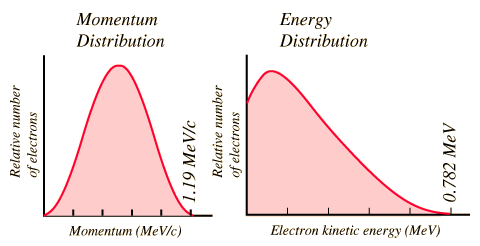
\includegraphics[scale=0.7]{nd}
  \caption{Electron properties in neutron decay in the rest frame. From \url{http://hyperphysics.phy-astr.gsu.edu/hbase/Particles/proton.html}}
  \label{fig:nd}
\end{figure}


\section{Backup}
\label{sec:backup}

Perturbation theory is developed more easily using the Hamiltonian formalism. We therefore consider a general field theory with a Hamiltonian
\begin{align}
  \label{eq:75}
  H=H_0+H_{\text{int}}\,
\end{align}
where $H_0$ is the free Hamiltonian and $H_{\text{int}}$ is the interaction term. The interaction term will be considered small. For instance in QED
\begin{align}
  H_{\text{int}}=\int d^3x\,\mathcal{H}_{\text{int}}=-\int d^3x\,\mathcal{L}_{\text{int}}
\end{align}
with
\begin{align}
  \mathcal{L}_{\text{int}}=-e A_\mu\overline{\psi}\gamma^\mu\psi
\end{align}
The smallnes of the interaction follows from the fact that the parameter which turns out to be relevatn for the perturbation expansion is $\alpha=e^2/4\pi\approx1/137$.


\begin{align}
  S S^\dagger=&(1+i T)(1-i T^\dagger)\nonumber\\
  &=1+i(T-T^\dagger)+T T^\dagger=1\,,\nonumber\\
\end{align}
\begin{align}
  T T^\dagger=-i(T-T^\dagger)\,.
\end{align}
Inserting a complete set of states we have
\begin{align}
  \langle b|T T^\dagger|a\rangle=&-i(\langle b|T|a\rangle-\langle b|T^\dagger|a\rangle)\nonumber\\
\langle b|T\left(\sum_n|n\rangle\langle n|\right)T^\dagger|a\rangle=&-i\left[\langle b|T|a\rangle-\left(\langle a|T|b\rangle\right)^\dagger\right]\nonumber\\
\sum_n\langle b|T|n\rangle\langle a|T|n\rangle^\dagger=&-i\left(\langle b|T|a\rangle-\langle a|T|b\rangle^*\right)\nonumber\\
\sum_n T_{bn}T_{an}^*=&-i\left(T_{ba}-T_{ab}^*\right)\,.\nonumber\\
\end{align}
if $a=b$
\begin{align}
  |T_{an}|^2=-i\operatorname{Im}T_{aa} \,.
\end{align}

%\left(\right)
%%% Local Variables: 
%%% mode: latex
%%% TeX-master: "beyond"
%%% End:
%instiki:category: QuantumFieldTheory
\chapter{Two body decays}
\label{cha:two-body-decays} %noinstiki
%instiki:
%instiki:***
%instiki:
%instiki:[[Beyond|Contents]]
%instiki:
%instiki:***
%instiki:
%instiki:* [Particle decays](#particle-decays)
%instiki:
%instiki:* [Width decay](#width-decay)
%instiki:
%instiki:* [Feynman Rules and trace theorems](#feynman-rules-trace)
%instiki:

In this chapter we use directly the Feynman rules for Fermions to carry out the calculation of the decay of the standard model Higgs into a pair of fermions. In chapter \ref{chap:fr} we will obtain the corresponding Feynman rules from the $S$--matrix expansion.




\section{Particle decays}
\label{sec:particle-decays}

Particle decay \cite{PD}  is the spontaneous process of one elementary particle transforming into other elementary particles. During this process, an elementary particle becomes a different particle with less mass and an intermediate particle such as $W$ boson in muon decay. 

For a particle of a mass $M$,  the differential decay width according Eq.~\eqref{eq:51}, is
\begin{equation}
  \label{eq:76}
 d\Gamma_n = \frac{(2\pi)^4}{2M}\left|\mathcal{M}\right|^2 d \Phi^{(n)} (P; p_1, p_2,\dots, p_n) \,
\end{equation}
The phase space can be determined from Eq.~\eqref{eq:50}
\begin{equation}
  d \Phi^{(n)} (P; p_1, p_2,\dots, p_n) = \delta^4 (P - \sum_{i=1}^n p_i) \left( \prod_{i=1}^n \frac{d^3 p_i}{(2\pi)^3 2 E_i} \right)\,.
\end{equation}
We will keep the $d\Gamma$ notation until all the integrals get evaluated. 

The two-body decays in eq.~\eqref{eq:152} is 
\begin{align}
\label{eq:154pd}
\frac{d\Gamma}{d\Omega}=
&\frac{1}{64 \pi^2M^3}\left|\mathcal{M}_{fi}\right|^2\lambda^{1/2}(M^2,m_2^2,m_1^2)
\end{align}



\section{Width decay}
\label{sec:width-decay}
%Poner las reglas de Feynman Aqui

Reglas de Feynman: Time direction from left to right.
\begin{itemize}
\item Initial particle: ${u}(p)$ 
\includegraphics{frip}
\item Initial antiparticle: $\bar{v}(p)$ 
\includegraphics{fria}
\item Final particle: $\bar{u}(p)$ 
\includegraphics{frfp}
\item Final antiparticle: ${v}(p)$ 
\includegraphics{frfa}

\end{itemize}

We consider now a general Yukawa interaction term
\begin{align}
  \mathcal{L}_{\text{int}}=hH\overline{f}_1 f_2
\end{align}
For the $H\to \overline{f}_1f_2$ decay.
The interaction between the Higgs boson with fermions\footnote{In this case we consider only electrons, by the formula is easy generalizable to other fermions} is given by the Yukawa interaction term \cite{lsm}
\begin{align}
\label{eq:155l}
\mathcal{L}_{\text{Higgs}}&=-G_{f}\frac{(v+H)}{\sqrt{2}}(\overline{f}_{R}f_{L}+\overline{f}_{L}f_{R})\nonumber\\
&=-\frac{G_{f}v}{\sqrt{2}}\overline{f}f-\frac{G_{f}H}{\sqrt{2}}\overline{f}f\nonumber\\
&=-m_f\overline{f}f-m_f\left(G_{F}\sqrt{2}\right)^{1/2}\overline{f}f
\end{align}
Such as the electro has acquired a mass $m_{e}=G_{f}\nu/\sqrt{2}$. On the other hand the coupling to be assigned to the process vertex is 
$G_{f}\sqrt{2}$ or $m_{f}/v=$. 

The decay process $H\to f\overline{f}$, is displayed in Fig. 
\ref{fig:a} %noinstiki

\begin{figure}[h!] %noinstiki
\begin{center} %noinstiki
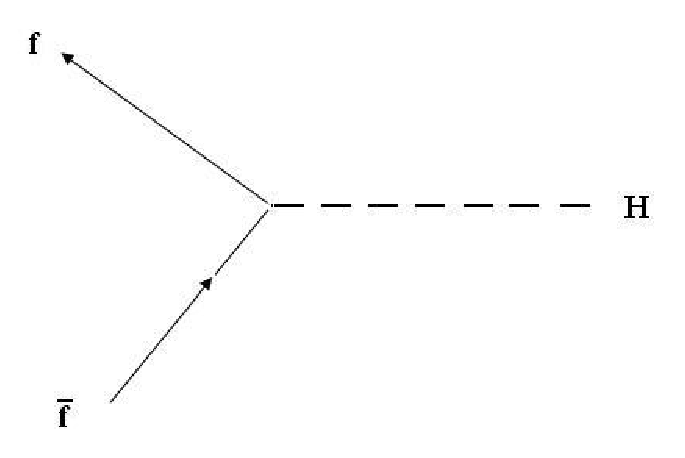
\includegraphics[scale=0.5]{decay}%noinstiki
\caption{Diagrama de proceso $H\to f\overline{f}$} %noinstiki
\label{fig:a} %noinstiki
\end{center} %noinstiki
\end{figure} %noinstiki

The Feynman rules, to be explained in Chapter~\ref{chap:fr} are indicated in Fig. 
\ref{fig:b}. %noinstiki

\begin{figure}[h] %noinstiki
\begin{center} %noinstiki
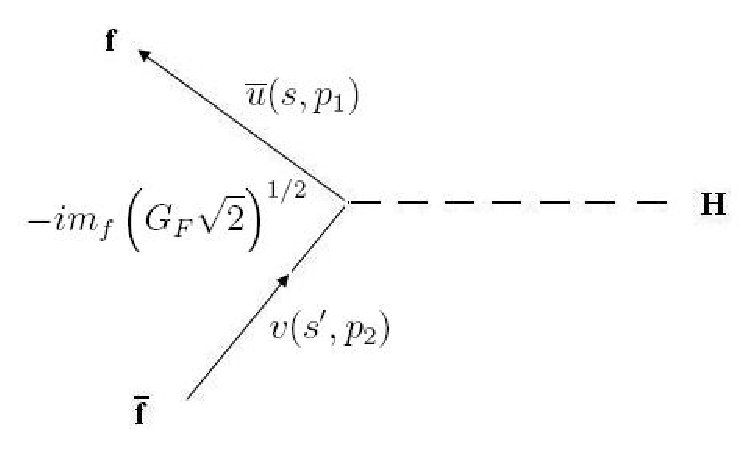
\includegraphics[scale=0.65]{feyn}%noinstiki
\caption{Reglas de Feynman del proceso $H\to f\overline{f}$}%noinstiki
\label{fig:b} %noinstiki
\end{center} %noinstiki
\end{figure} %noinstiki

In this way the scattering amplitude is 
\begin{equation}
i\mathcal{M}=-im_{f}\left(G_{F}\sqrt{2}\right)^{1/2}\overline{u}(s_1,
p_{1})v(s_2, p_{2}). 
\end{equation}
where $p_{1}$, $s$,  $p_{2}$ y $s_2$ are the momentum and spines of fermion and anti--fermion respectively.

For the general case
\begin{align}
i\mathcal{M}=-i h\overline{u}(s_1,p_{1})v(s_2, p_{2}). 
\end{align}
$h=m_{f}\left(G_{F}\sqrt{2}\right)^{1/2}$ in the standard models
Now, having into account that ${\gamma^{0}}^{\dag}=\gamma^{0}$
\begin{align*}
&(\overline{u}(s_1,p_{1})v(s_2, p_{2}))^{\dag}\\
&=v^{\dag}(s_2, p_{2})(\overline{u}(s_1,p_{1}))^{\dag}\\
&=v^{\dag}(s_2, p_{2})({u^{\dag}}(s_1,p_{1}){\gamma^{0}})^{\dag}\\
&=v^{\dag}(s_2, p_{2})({\gamma^{0}}^{\dag}u(s_1,p_{1}))\\
&=v^{\dag}(s_2, p_{2})(\gamma^{0}u(s_1,p_{1}))\\
&=\overline{v}(s_2,p_{2})u(s_1,p_{1}). 
\end{align*}
Squaring  $\mathcal{M}$,  and summing over possible polarization states of final particles, we have

\begin{equation}
\sum_{s_1,s_2}|\mathcal{M}|^{2}=h^2\sum_{s_1,s_2}(\overline{u}(s_1,p_{1})v(s_2,
p_{2}))(\overline{v}(s_2,p_{2})u(s_1,p_{1})). \label{eq:80}
\end{equation}
The several sums in Ec.~(\ref{eq:80}) can be calculated by expressing the products  $\overline{u}v$ y $\overline{v}u$ en in terms of their components, as follow
\begin{align}
\label{eq:81}
&\sum_{s_1,s_2}(\overline{u}(s_1,p_{1})v(s_2, p_{2}))(\overline{v}(s_2,p_{2})u(s_1,p_{1}))\nonumber\\
&=\sum_{s_1,s_2}(\overline{u}_{\alpha}(s_1,p_{1})v_{\alpha}(s_2, p_{2}))(\overline{v}_{\beta}(s_2,p_{2})u_{\beta}(s_1,p_{1}))\nonumber\\
&=\sum_{s_1,s_2}(u_{\beta}(s_1,p_{1})\overline{u}_{\alpha}(s_1,p_{1}))(v_{\alpha}(s_2, p_{2})\overline{v}_{\beta}(s_2,p_{2}))\nonumber\\
&=\sum_{s}u_{\beta}(s_1,p_{1})\overline{u}_{\alpha}(s_1,p_{1})\sum_{s_2}v_{\alpha}(s_2, p_{2})\overline{v}_{\beta}(s_2,p_{2})\nonumber\\
&=(\cancel{p}_{1}+m_{f})_{\beta\alpha}(\cancel{p}_{2}-m_{f})_{\alpha\beta}\nonumber\\
&=\operatorname{Tr}[(\cancel{p}_{1}+m_{f})(\cancel{p}_{2}-m_{f})]. 
\end{align}
Taking into account that  $\operatorname{Tr}[\gamma_{\nu}]=0$, and from the commutation relations for $\gamma_\mu$ matrices
\begin{align*}
\operatorname{Tr}[\gamma_{\mu}\gamma_{\nu}]&=\operatorname{Tr}[-\gamma_{\nu}\gamma_{\mu}+2g^{\mu\nu}]\\
&=\operatorname{Tr}[-\gamma_{\nu}\gamma_{\mu}]+2g^{\mu\nu}\operatorname{Tr}[\mathbf{1}]\\
&=\operatorname{Tr}[-\gamma_{\mu}\gamma_{\nu}]+2g^{\mu\nu}4 \qquad (\operatorname{Tr}[AB]=\operatorname{Tr}[BA])\\
\operatorname{Tr}[\gamma_{\mu}\gamma_{\nu}]&=4g^{\mu\nu}.
\end{align*}

In this way
\begin{align*}
&\operatorname{Tr}[(\cancel{p}_{1}+m_{1})(\cancel{p}_{2}-m_{2})]\\
&=\operatorname{Tr}[(\gamma_{\mu}p^{\mu}_{1}+m_{1})(\gamma_{\nu}p^{\nu}_{2}-m_{1})]\\
&=\operatorname{Tr}[\gamma_{\mu}\gamma_{\nu}p^{\mu}_{1}p^{\nu}_{2}-m_{2}\gamma_{\mu}p^{\mu}_{1}+m_{1}\gamma_{\nu}p^{\nu}_{2}-m_{1}m_2]\\
&=p^{\mu}_{1}p^{\nu}_{2}\operatorname{Tr}[\gamma_{\mu}\gamma_{\nu}]-4m_1 m_2\\
&=4g_{\mu\nu}p^{\mu}_{1}p^{\nu}_{2}-4m_1m_2\\
&=4(p_{1}\cdot p_{2}-m_1m_2). 
\end{align*}
where  $m_1$, $m_2$ are the final masses, and
\begin{equation*}
\sum_{s_1,s_2}|\mathcal{M}|^{2}=4h^2(p_{1}\cdot p_{2}-m_{1}m_2).
\end{equation*}
From eq.~\eqref{eq:153}
\begin{align}
  M=&E_1+E_2\nonumber\\
|\mathbf{p}_1|&=|\mathbf{p}_2|
\end{align}
Therefore
\begin{align}
  E_1E_2=\frac{M^2-E_1^2-E_2^2}{2}
\end{align}
\begin{align*}
p_{1}\cdot p_{2}-m^{2}_{f}&=E_{1}E_{2}-\mathbf{p}_{1}\cdot\mathbf{p}_{2}-m_1 m_2\\
&=E_{1}E_{2}+\mathbf{p}_{1}^2-m_1 m_2\\
&=\frac{M^2-E_1^2-E_2^2}{2}+\mathbf{p}_{1}^2-m_1 m_2\nonumber\\
&=\frac12\left(M^2-m_1^2-\mathbf{p}_1^2-m_2^2-\mathbf{p}_1^2\right)+\mathbf{p}_{1}^2-m_1 m_2\\
&=\frac12\left(M^2-m_1^2-m_2^2-2m_1m_2\right)\\
&=\frac12\left[M^2-(m_1-m_2)^2\right]
\end{align*}
%\left(\right)
Therefore, the scattering  amplitude is
\begin{equation}
\sum_{s_1,s_2}|\mathcal{M}|^{2}=2h^2\left[M^2-(m_1+m_2)^2\right]
\label{eq:82}
\end{equation}
Replacing back in eq.~\eqref{eq:154pd}
\begin{align}
\frac{d\Gamma}{d\Omega}=
&\frac{h^2}{32 \pi^2M^3}\lambda^{1/2}(M^2,m_2^2,m_1^2)\left[M^2-(m_1+m_2)^2\right]
\end{align}
After the integration $\int d\Omega_{\text{CM}}=4\pi$\footnote{$\int_0^{2\pi}d\phi\int_0^\pi\sin\theta d\theta=4\pi $} we have
\begin{align}
\Gamma=&\frac{h^2}{8 \pi M^3}\lambda^{1/2}(M^2,m_2^2,m_1^2)\left[M^2-(m_1+m_2)^2\right]
\end{align}
For $m_1=m_2=m_f$
\begin{align}
  \lambda^{1/2}(M^2,m_2^2,m_1^2)=&M^2\left(1-\frac{4m_f^2}{M^2}\right)^{1/2}\nonumber\\
\left[M^2-(m_1+m_2)^2\right]=&M^2\left(1-\frac{4m_f^2}{M^2}\right)
\end{align}
and therefore
\begin{align}
\Gamma(H\to f\overline{f})=&\frac{h^2}{8 \pi}M\left(1-\frac{4m_f^2}{M^2}\right)^{3/2}
\end{align}
In the case of the standard model Higgs with mass $M_H$ decaying to fermion pair, according to the Lagrangian in eq.~\eqref{eq:155l}

\begin{equation}
\Gamma(H\to f\overline{f})=\frac{M_{H}m_{f}^{2}G_{F}}{4\pi\sqrt{2}}
\left(1-4\frac{m^2_{f}}{M^2_{H}}\right)^{3/2}, 
\end{equation}

In the limit $m_{f}\ll M_{H}$ this expression reduces to 
\begin{equation}
\Gamma(H\to
f\overline{f})=\frac{M_{H}m_{f}^{2}G_{F}}{4\pi\sqrt{2}}. 
\end{equation}


\section{$e^+ e^- \to \mu^+\mu^-$}

\begin{align}
  \mathcal{L}=\frac{e^2}{s}
  \left[\bar v(k_2)\gamma^\lambda u(k_1)  \right]
  \left[\bar v(k_2)\gamma^\lambda u(k_1)  \right]
\end{align}

%%% Local Variables: 
%%% mode: latex
%%% TeX-master: "beyond"
%%% End:
%instiki:category: QuantumFieldTheory
\chapter{Feynman Rules}
\label{chap:fr} %noinstiki
%instiki:
%instiki:***
%instiki:
%instiki:[[Beyond|Contents]]
%instiki:
%instiki:***
%instiki:
%instiki:* [Interaction picture](#interaction-picture)
%instiki:
%instiki:* [Yukawa interaction](#feynman-diagrams)
%instiki:
%instiki:* [Scattering](#scattering)
%instiki:

When the case of interacting fields are considered, the particles can be created, destroyed and scattered. In essence this requires solving the coupled non-linear field equations for given conditions. This is an extremely difficult problem which has only been solved in perturbation theory.

In the Heisenberg picture, which we have so far been using, this program is still very complex, and it was decisive for the successful development of the theory to work instead in the interaction picture. In section \ref{sec:interaction-picture} we write the $S$--matrix expansion derived in Chapter~\ref{cha:s-matrix}, in the interaction picture. In section \ref{sec:feynman-diagrams} we show how to use the Wick expansion to calculate $S$--matrix elements involving scalars and spinors.

\section{Interaction picture}
\label{sec:interaction-picture}
This part is based in \cite{Mandl:1985bg}. 
In the Schr\"odinger Picture (SP) the time dependence is carried by the states according to the Scr\"odinger equation 
\begin{align}\
label{eq:84f}
  i\frac{\partial}{\partial t}|a,t\rangle_{\text{S}}=  i\frac{d}{dt}|a,t\rangle_{\text{S}}=  {H}|a,t\rangle_{\text{S}}
\end{align}
With the solution given in Eq.~\eqref{eq:39f}
\begin{align}
\label{eq:85f}
    |a,t\rangle_{\text{S}}=U(t,t_i)|a\rangle_{\text{S}}\,.
\end{align}
where $U$ is the unitary operator [see Eq.~\eqref{eq:40f}]
\begin{align}
 U\equiv U(t,t_i)= e^{-i H(t-t_i)}\,.
\end{align}
Given the state $|a,t\rangle_{\text{S}}$ in the SP, in the Heisenberg picture (HP) we defined the state
\begin{align}
\label{eq:86f}
  |a\rangle_H=U^\dagger|a,t\rangle_{\text{S}}=|a\rangle_{\text{S}}
\end{align}
Si $O^{\text{S}}$ in an operator in the SP, the corresponding Heisenberg operator is defined as
\begin{align}
\label{eq:87f}
  O^{\text{H}}(t)=U^\dagger O^{\text{S}}U
\end{align}
Hence, the transformation from HP to SP is unitary. At $t=t_i$, states and operators in the two pictures are the same. We see from Eq.~\eqref{eq:86f} that in the HP state vectors are constant in time, while from Eq.~\eqref{eq:87f} the Heisenberg operators evolve with time. Is convenient to keep the temporal label in the Heisenberg states
\begin{align}
  |a\rangle_H=|a,t_i\rangle_H
\end{align}
Eq.~\eqref{eq:87f} ensures the invariance of matrix elements and commutation relations:
\begin{align}
  {}_{\text{S}}\langle b,t|\,O^{\text{S}}\,|a,t\rangle_{\text{S}}=  {}_{\text{S}}\langle b,t|\,U O^{\text{H}}(t) U^\dagger\,|a,t\rangle_{\text{S}}=
{}_{\text{H}}\langle b,t_i|O^{\text{H}}(t)|a,t_i\rangle_{\text{H}}
\end{align}
\begin{align}
\left[O^{\text{S}},P^{\text{S}}\right]=c\Rightarrow\left[O^{\text{H}}(t),P^{\text{H}}(t)\right]=c
\end{align}
where $c$ is a constant.

Differentiation of Eq. \eqref{eq:87f} 
\begin{align}
  \frac{d}{dt}O^{\text{H}}(t)=&\left(\frac{d}{dt}U^\dagger\right)O^{\text{S}}U+
U^\dagger O^{\text{S}}\frac{d}{dt}U\nonumber\\
 =&i H\, U^\dagger O^{\text{S}}U+
U^\dagger O^{\text{S}}U(-i H)\nonumber\\
 =&-i ( O^{\text{H}}H-H O^{\text{H}})\,,
\end{align}
gives the Heisenberg equation of motion

\begin{align}
  i\frac{d}{dt}O^{\text{H}}(t)=\left[O^{\text{H}}(t),H\right]
\end{align}
The interaction picture (IP) arises if the Hamiltonian is split into two parts
\begin{align}
  H=H_0+H_{\text{I}}\,.
\end{align}
In quantum field theory $H_I$ will describe the interaction between two fields, themselves described by $H_0$

IP is related to the SP by the unitary transformation
\begin{align}
\label{eq:88f}
  U_i\equiv U_i(t,t_i)=e^{-i H_i(t-t_i)}\,,
\end{align}
in this way,
\begin{align}
\label{eq:89f}
  |a,t\rangle_{\text{I}}=U_0^\dagger|a,t\rangle_{\text{S}}\,,
\end{align}
and
\begin{align}
\label{eq:90f}
  O^{\text{I}}(t)=U^\dagger_0 O^{\text{S}}U_0\,.
\end{align}
Thus the relation between IP and SP is similar to that between HP and SP, but with the unitary transformation $U_0$ involving only the non--interacting Hamiltonian $H_0$. Note that both the vector states as the operators in the IP are time-dependent.

Differentiating Eq.~\eqref{eq:90f} gives the differential equation of motion operators in the IP:
\begin{align}
  i\frac{d}{dt}O^{\text{I}}(t)=\left[O^{\text{I}}(t),H_0\right]
\end{align}

Substituting Eq.~\eqref{eq:89f} into the Scr\"odinger Eq.~\eqref{eq:84f}, one obtains the equation of motion of state vectors in the IP, If the system is described by a time-dependent state vector $|\Phi(t)\rangle$
\begin{align}
  i\frac{d}{dt}|a,t\rangle_{\text{S}}=&  H^{\text{S}}|a,t\rangle_{\text{S}}\nonumber\\
  i\frac{d}{dt}\left(U_0|\Phi(t)\rangle\right)=&  H^{\text{S}}U_0|\Phi(t)\rangle\nonumber\\
  i\left(\frac{d}{dt}U_0\right)|\Phi(t)\rangle+iU_0\frac{d}{dt}|\Phi(t)\rangle=&  H^{\text{S}}U_0|\Phi(t)\rangle\nonumber\\
  U_0 H_0|\Phi(t)\rangle+iU_0\frac{d}{dt}|\Phi(t)\rangle=&  H^{\text{S}}U_0|\Phi(t)\rangle\nonumber\\
  U_0 H_0|\Phi(t)\rangle+iU_0\frac{d}{dt}|\Phi(t)\rangle=&  (H_0+H_I^{\text{S}})U_0|\Phi(t)\rangle\nonumber\\
  iU_0\frac{d}{dt}|\Phi(t)\rangle=&  H_I^{\text{S}}U_0|\Phi(t)\rangle\nonumber\\
  i\frac{d}{dt}|\Phi(t)\rangle=& U_0 H_I^{\text{S}}U_0|\Phi(t)\rangle
\end{align}
\begin{align}
\label{eq:91f}
  i\frac{d}{d t}|\Phi(t)\rangle_{\text{I}}=H^{\text{I}}_I\,|\Phi(t)\rangle_{\text{I}}\,,
\end{align}
where, as in Eq.~\eqref{eq:90f}
\begin{align}
  \label{eq:92f}
  H^{\text{I}}_I=e^{i H_0^{{\text{S}}}(t-t_i)}H^{\text{S}}_I e^{-i H_0^{{\text{S}}}(t-t_i)}
\end{align}
is the interaction Hamiltonian in the IP, with $H^{\text{S}}_I$ and $H^{\text{S}}_0$ being the interaction and free-field Hamiltonian in the SP. From now on we shall omit the labels I, used in the equations to distinguish the IP, as we shall be working exclusively in the IP in what follows.

Eq. \eqref{eq:91f} is a Scr\"odinger-like equation with the time dependent Hamiltonian $H_I(t)$. With the interaction switched off (i.e.  we put $H_I=0$), the state vector is constant in time. The interaction leads to the state $|\Phi(t)\rangle$ changing with time. Given that the system is in a state  $|i\rangle$ at an initial time $t=t_i$, i.e.
\begin{align}
\label{eq:93f}
  |\Phi(t_i)\rangle=|i\rangle\,,
\end{align}
the solution of Eq.~\eqref{eq:91f} with this initial condition gives the state $|\Phi(t)\rangle$ of the system at any other time $t$. It follows from the Hermicity of the operator $H_I(t)$ that the time development of the state $|\Phi(t)\rangle$ according to Eq.~\eqref{eq:91f} is a unitary transformation. Accordingly it preserves the normalization of states
\begin{align}
  \langle\Phi(t)|\Phi(t)\rangle=\text{const}.
\end{align}
and, more generally, the scalar product.

Clearly the formalism which we are here developing is not appropriate for the description of bound states but it is particularly suitable for scattering processes. In a collision processes the state vector $|i\rangle$ will define an initial state, long before the scattering occurs ($t_i=-\infty$), by specifying a definite number of particles, with definite properties and far apart from each other so that they do not interact. (For example $|i\rangle$ would specify a definite number of electrons, and positrons with given momenta and spins). In the scattering process, the particles will come close together, collide (i.e interact) and fly apart gain. Eq.~\eqref{eq:91f} determines the state $|\Phi(t)\rangle$ into which the initial state
\begin{align}
  |\Phi(-\infty)\rangle=|i\rangle\,,
\end{align}
evolves at $t=\infty$, long after the scattering is over and all particles are for apart again. The $S$--matrix relates $|\Phi(\infty)\rangle$ to $\Phi(-\infty)$ and is defined by
\begin{align}
  |\Phi(\infty)\rangle=S|\Phi(-\infty)\rangle=S|i\rangle\,,
\end{align}

A collision can lead to many different final states $|f\rangle$, and all these possibilities are constrained within $|\Phi(\infty)\rangle$.

The transition probability is given by
\begin{align}
  \left|\langle f|\Phi(\infty)\rangle\right|^2=  \left|\langle f|S|i\rangle\right|^2\equiv S_{f i}^2\,,
\end{align}
where $S_{f i}$ is the corresponding probability amplitude.

In order to calculate the $S$--matrix we must solve Eq.~\eqref{eq:91f} for the initial condition \eqref{eq:93f}. These equations can be combined into the integral equation
\begin{align}
 d |\Phi(t)\rangle=&-i d t\,H_I(t)|\Phi(t)\rangle\nonumber\\
\int_{|\Phi(-\infty)\rangle}^{|\Phi(t)\rangle} d |\Phi(t)\rangle=&-i \int_\infty^t d t_1\,H_I(t_1)|\Phi(t_1)\rangle\nonumber\\
|\Phi(t)\rangle-|\Phi(-\infty)\rangle=&-i \int_\infty^t d t_1\,H_I(t_1)|\Phi(t_1)\rangle\nonumber\\
\end{align}

\begin{align}
\label{eq:94f}
  |\Phi(t)\rangle=|i\rangle-i\int_{-\infty}^t d t_1\,H_I(t_1)|\Phi(t_1)\rangle\,.
\end{align}
In the limit $t\to\infty$
\begin{align}
  |\Phi(\infty)\rangle=S^{(0)}|i\rangle-i\int_{-\infty}^\infty d t_1\,H_I(t_1)|\Phi(t_1)\rangle\,.
\end{align}
where 
\begin{align}
  S^{(0)}=1\,.
\end{align}
From Eq.~\eqref{eq:94f} we can obtain $|\Phi(t_1)\rangle$ at next order:
\begin{align}
  |\Phi(t_1)\rangle=&|i\rangle-i\int_{-\infty}^{t_1} d t_2\,H_I(t_2)|\Phi(t_2)\rangle\,.
\end{align}


This equation then can  be solved iteratively. If $H_I$ is small we can solve this equation by iteration
\begin{align}
\label{eq:95f}
  |\Phi(t)\rangle=|i\rangle+(-i)\int_{-\infty}^t d t_1 H_I(t_1)|i\rangle+(-i)^2\int_{-\infty}^t d t_1\int_{-\infty}^{t_1} d t_2\,H_I(t_1)H_I(t_2)|\Phi(t_2)\rangle\,.
\end{align}
In the limit $t\to\infty$
\begin{align}
  |\Phi(t)\rangle=&\left[S^{(0)}+(-i)\int_{-\infty}^\infty d t_1 H_I(t_1)\right]|i\rangle+(-i)^2\int_{-\infty}^\infty d t_1\int_{-\infty}^{t_1} d t_2\,H_I(t_1)H_I(t_2)|\Phi(t_2)\rangle\nonumber\\
  =&\left(S^{(0)}+S^{(1)}\right)|i\rangle+(-i)^2\int_{-\infty}^\infty d t_1\int_{-\infty}^{t_1} d t_2\,H_I(t_1)H_I(t_2)|\Phi(t_2)\rangle\,,
\end{align}
where 
\begin{align}
  S^{(1)}=(-i)\int_{-\infty}^\infty d t_1 H_I(t_1)\,.
\end{align}
The next order of Eq.~\eqref{eq:95f} is
\begin{align}
  |\Phi(t)\rangle=&|i\rangle+(-i)\int_{-\infty}^t d t_1 H_I(t_1)|i\rangle+(-i)^2\int_{-\infty}^t d t_1\int_{-\infty}^{t_1} d t_2\,H_I(t_1)H_I(t_2)\nonumber\\
  &\times\left[|i\rangle+(-i)\int_{-\infty}^{t_2} d t_3 H_I(t_3)|i\rangle+(-i)^2\int_{-\infty}^{t_2} d t_3\int_{-\infty}^{t_3} d t_4\,H_I(t_3)H_I(t_4)|\Phi(t_4)\rangle\right]
\end{align}
\begin{align}
  |\Phi(t)\rangle=&|i\rangle+(-i)\int_{-\infty}^t d t_1 H_1(t_1)|i\rangle+(-i)^2\int_{-\infty}^t d t_1\int_{-\infty}^{t_1} d t_2\,H_I(t_1)H_I(t_2)|i\rangle\nonumber\\
  &+(-i)^3\int_{-\infty}^t d t_1\int_{-\infty}^{t_1} d t_2\int_{-\infty}^{t_2} d t_3\,H_I(t_1)H_I(t_2) H_1(t_3)|i\rangle\nonumber\\
  &+(-i)^4\int_{-\infty}^t d t_1\int_{-\infty}^{t_1}d t_2 \int_{-\infty}^{t_2} d t_3\int_{-\infty}^{t_3}d t_4 \,H_I(t_1)H_I(t_2)\,H_I(t_3)H_I(t_4)|\Phi(t_4)\rangle
\end{align}
In the limit $t\to\infty$
\begin{align}
  |\Phi(t)\rangle=&\left(S^{(0)}+S^{(1)}+S^{(2)}+S^{(3)}\right)|i\rangle\nonumber\\
  &+(-i)^4\int_{-\infty}^\infty d t_1\int_{-\infty}^{t_1}d t_2 \int_{-\infty}^{t_2} d t_3\int_{-\infty}^{t_3}d t_4 \,H_I(t_1)H_I(t_2)\,H_I(t_3)H_I(t_4)|\Phi(t_4)\rangle
\end{align}
where
\begin{align}
  S^{(2)}=&(-i)^2\int_{-\infty}^\infty d t_1\int_{-\infty}^{t_1} d t_2\,H_I(t_1)H_I(t_2)\nonumber\\
  S^{(3)}=&(-i)^3\int_{-\infty}^\infty d t_1\int_{-\infty}^{t_1} d t_2\int_{-\infty}^{t_2} d t_3\,H_I(t_1)H_I(t_2) H_1(t_3)
\end{align}

and so on we obtain the $S$--matrix
\begin{align}
  S=&\sum_{n=0}^\infty S^{(n)}\nonumber\\
  =&1+\sum_{n=1}^\infty\frac{(-i)^n}{n!}\int_{-\infty}^{\infty}d t_1\,\int_{-\infty}^{t_1} d t_2\ldots\int_{-\infty}^{t_{n-1}}d t_n\,{H}_I(t_1){H}_I(t_2)\ldots{H}_I(t_n)\,.
\end{align}


\section{Atomic decay}
\label{sec:atomic-decay}

Here we follow closelly \cite{Gross:1993} chapter 3.

For the atomic decay at first order in perturbation theory, we have
\begin{align}
  S_{\beta\alpha}^{(1)}=-i \int_{-\infty}^\infty dt\, \left\langle\beta\left|H_I(t)\right|\alpha\right\rangle.
\end{align}
where the Hamiltonian in the interaction picture is
\begin{align}
  H=&H_A+H_{EM}+H_I(t)=H_0+H_I(t)\,,
\end{align}
where, following the definition of the interaction picture
\begin{align}
  \psi_a(r,t)=&e^{-i H_A t}\psi_a(r)\nonumber\\
=&U_A(t)\psi_a(r)\,,
\end{align}

\begin{align}
  H_I(t)=U_A^{-1}H'_I(t)U_A\,.
\end{align}
The several terms of the Hamiltonia are

\begin{align}
  H_A=\frac{\mathbf{p}_e^2}{2m}-\frac{Z\alpha}{r_e}\,,
\end{align}
\begin{align}
  H_{EM}=\frac{1}{2}\int d^3r\left\{:\boldsymbol{\pi}^2(r,t):+:\mathbf{B}^2(r,t):\right\}\,,
\end{align}
\begin{align}
  H_I'(t)=\left\{\frac{e}{2m}\left(\mathbf{p}_e\cdot\mathbf{A}(r_e,t)+\mathbf{A}(r_e,t)\cdot \mathbf{p}_e
+\frac{e^2}{2m}\mathbf{A}^2(r_e,t)\right)\right\}\,,
\end{align}
and $\alpha=e^2/(4\pi)$.
The states as defined as
\begin{align}
  |a,n\rangle=\psi_a(r_e)|n\rangle\,.
\end{align}
The scalar product of the atomic states requires an integration over the coordinate $r_e$
\begin{align}
  \label{eq:163f}
   \langle a',n'|a,n\rangle=\int d^3r\,\psi_{a'}^*(r_e)\psi_a(r_e)\langle n'|n\rangle.
\end{align}

For one photon decay of an initial atomic state $a$ into a final atomic state $b$ and a photon of energy $\omega_n$ and polarization $\lambda$, the states are
\begin{align}
  |\alpha\rangle=&|\alpha,0\rangle=\psi_a(r_e)|0\rangle\nonumber\\
  |\beta\rangle=&|b,1_{n\lambda}\rangle=\psi_b(r_e)|1_{n\lambda}\rangle\,,
\end{align}
where
\begin{align}
  |1_{n\lambda}\rangle=a_{n\lambda}^\dagger|0\rangle
\end{align}
is the one-photon state with frequency $\omega_n$ and polarization $\lambda$. Since
\begin{align}
 \langle1_{n\lambda}|\mathbf{A}^2|0\rangle\supset\langle1_{n\lambda}|(a_{n\lambda}^\dagger a_{n\lambda}^\dagger+a_{n\lambda}^\dagger a_{n\lambda}+a_{n\lambda}a_{n\lambda})|0\rangle=\langle0|1_{n\lambda}\rangle=0
\end{align}
and
\begin{align}
\left(\mathbf{p}_e\cdot\mathbf{A}(r_e,t)+\mathbf{A}(r_e,t)\cdot \mathbf{p}_e\right)\psi_a(r_e)=&
-i\left(\boldsymbol{\nabla}_e\cdot\mathbf{A}(r_e,t)+\mathbf{A}(r_e,t)\cdot\boldsymbol{\nabla}_e\right)\psi_a(r_e)
\nonumber\\
=&-i\left\{\left(\boldsymbol{\nabla}_e\cdot\mathbf{A}\right)\psi_a
+\mathbf{A}\cdot\boldsymbol{\nabla}_e\psi_a
+\mathbf{A}\cdot\boldsymbol{\nabla}_e\psi_a\right\}\nonumber\\
=&-i\left\{2\mathbf{A}\cdot\boldsymbol{\nabla}_e\psi_a\right\}\,,
\end{align}
where $\boldsymbol{\nabla}\cdot\mathbf{A}=0$ was used.

With all of this we have a simplified formula
\begin{align}
\label{eq:164f}
  S_{ba}=&-i\int_{-\infty}^\infty dt\langle b,1_{n\lambda}|U_A^{-1}\left(-\frac{ie}{m}\mathbf{A}(r_e,t)\cdot\boldsymbol{\nabla}_e\right)
  U_A|a,0\rangle\nonumber\\
  S_{ba}=&-i\int_{-\infty}^\infty dt\langle b,1_{n\lambda}|U_A^{-1}\left(-\frac{ie}{m}\mathbf{A}(r_e,t)\cdot\boldsymbol{\nabla}_e\right)
  U_A|a,0\rangle\nonumber\\
  S_{ba}=&-i\int_{-\infty}^\infty dt\langle b,1_{n\lambda}|e^{iE_b t}\left(-\frac{ie}{m}\mathbf{A}(r_e,t)\cdot\boldsymbol{\nabla}_e\right)
  e^{-i E_a t}|a,0\rangle\nonumber\\
  =&-\int_{-\infty}^\infty dt\,e^{i(E_b-E_a)t}\int d^3r_e\langle1_{n\lambda}|\psi_b^*(r_e)\frac{e}{m}\left(\mathbf{A}(r_e,t)\cdot\boldsymbol{\nabla}_e\right)
  \psi_a(r)|0\rangle\nonumber\\
 =&-\int_{-\infty}^\infty dt\,e^{i(E_b-E_a)t}\frac{e}{m}\int d^3r_e\left\{\psi_b^*(r_e)\boldsymbol{\nabla}_e\psi_a(r)\right\}\cdot 
  \langle1_{n\lambda}|\mathbf{A}(r_e,t)|0\rangle.
\end{align}
Since
\begin{align}
  \langle1_{n\lambda}|\mathbf{A}(r_e,t)|0\rangle=&\sum_{n'\lambda'}\frac{1}{\sqrt{2\omega_{n'}L^3}}\boldsymbol{\epsilon}^{\lambda'}_{n'}
  \langle1_{n\lambda}|a^\dagger_{n'\lambda'}|0\rangle e^{i k_{n'}\cdot x_e}\nonumber\\
=&\sum_{n'\lambda'}\frac{1}{\sqrt{2\omega_{n'}L^3}}\boldsymbol{\epsilon}^{\lambda'}_{n'}
  \langle1_{n\lambda}|a^\dagger_{n'\lambda'}|0\rangle e^{i k_{n}\cdot x_e}\nonumber\\
=&\frac{1}{\sqrt{2\omega_{n}L^3}}\boldsymbol{\epsilon}^{\lambda}_{n}
  \langle1_{n\lambda}|1_{n\lambda}\rangle e^{i k_{n'}\cdot x_e}\nonumber\\
=&\frac{1}{\sqrt{2\omega_{n}L^3}}\boldsymbol{\epsilon}^{\lambda}_{n}
  e^{i \omega_n t-\mathbf{k}_n\cdot\mathbf{r}_e}\,.
\end{align}
Inserting this expression into (\ref{eq:164f}) gives
%%% faltan detalles
\begin{align}
  S_{ba}=-i2\pi \delta(E_b+\omega_n-E_a)\frac{1}{\sqrt{L^3}}M_{ba}\,, 
\end{align}
where the decaya amplitude $M_{ba}$ is
\begin{align}
  M_{ba}=-i\frac{e}{m}\frac{1}{2\omega_n}\int d^3r_e\,e^{-i\mathbf{k}_n\cdot\mathbf{r}_e}
  \psi_b^*(r_e)\boldsymbol{\epsilon}^{\lambda}_{n}\cdot\boldsymbol{\nabla}_e\psi_a(r)\,.
\end{align}
In most atomic decays, the energy of the emmited photon, which is equal to $\omega_n=E_b-E_a$, is much less than $1/R$, where $R$ is the
size of the atomic system, and hence the maximum range of the integral over $r_e$. In this case, the dipole approximation 
\begin{align}
  e^{-i\mathbf{k}_n\cdot\mathbf{r}_e}\approx1
\end{align}
is extremely good. Then we have
\begin{align}
  M_{ba}=\frac{e}{m}\frac{1}{\sqrt{2\omega_n}}\boldsymbol{\epsilon}^{\lambda}_{n}\cdot\mathbf{p}_{ba}\,,
\end{align}
where
\begin{align}
  \mathbf{p}_{ba}=-i\int d^3r_e \psi_b^*(r_e)\boldsymbol{\nabla}_e\psi_a(r_e).
\end{align}
The diferential decay rate, and using
\begin{align}
  [2\pi \delta(E_f-E_i)]^2=2\pi \delta(E_f-E_i) T \,,
\end{align}
we have
\begin{align}
  \Delta W_{ba}=&\lim_{T\to \infty}\frac{|S_{ba}(T/2,-T/2)|^2}{T}\nonumber\\
  =&\lim_{T\to \infty}\frac{1}{T}2\pi \delta(E_b+\omega_n-E_a) T \frac{1}{L^3}|M_{ba}|^2\nonumber\\
  =&2\pi\delta(E_b+\omega_n-E_a)\frac{1}{L^3}|M_{ba}|^2
\end{align}
Then
\begin{align}
  \Delta W_{ba}=&\frac{2\pi}{V}\delta(E_b+\omega_n-E_a)\frac{e^2}{2\omega_n m^2}|\boldsymbol{\epsilon}^{\lambda}_{n}\cdot\mathbf{p}_{ba}|^2\,.
\end{align}
Summing over all final photon states to get the total $a\to b$ decay rate gives
\begin{align}
  W_{ba}=&\sum_{n,\lambda}\frac{2\pi}{V}\delta(E_b+\omega_n-E_a)\frac{e^2}{2\omega_n m^2}|\boldsymbol{\epsilon}^{\lambda}_{n}\cdot\mathbf{p}_{ba}|^2\nonumber\\
  =&\sum_{\lambda}\sum_n\frac{2\pi}{V}\delta(E_b+\omega_n-E_a)\frac{e^2}{2\omega_n m^2}|\boldsymbol{\epsilon}^{\lambda}_{n}\cdot\mathbf{p}_{ba}|^2\,.
\end{align}
Using
\begin{align}
  \sum_n\to \frac{V}{(2\pi)^3}\int d^3k
\end{align}
\begin{align}
   W_{ba}=&\sum_{\lambda}\int\frac{d^3k}{(2\pi)^2}\delta(E_b+\omega_n-E_a)\frac{e^2}{2\omega m^2}|\boldsymbol{\epsilon}^{\lambda}_{n}\cdot\mathbf{p}_{ba}|^2\nonumber\\
=&\frac{e^2}{2m^2}\sum_{\lambda}\int\frac{d^3k}{(2\pi)^2\omega}\delta(E_b+\omega_n-E_a)|\boldsymbol{\epsilon}^{\lambda}_{n}\cdot\mathbf{p}_{ba}|^2\nonumber\\
=&\frac{e^2}{2m^2}\sum_{\lambda}\int|\mathbf{k}|^2d|\mathbf{k}|\int d\Omega\frac{d^3k}{(2\pi)^2\omega}\delta(E_b+\omega-E_a)|\boldsymbol{\epsilon}^{\lambda}_{n}\cdot\mathbf{p}_{ba}|^2\,.
\end{align}
By using $|\mathbf{k}|=\omega$, we have
\begin{align}
  W_{ba}=&\frac{e^2}{2m^2}\sum_{\lambda}\int d\omega\frac{\omega}{(2\pi)^2}\delta(E_b+\omega-E_a)\int d\Omega|\boldsymbol{\epsilon}^{\lambda}_{n}\cdot\mathbf{p}_{ba}|^2\nonumber\\
=&\frac{e^2}{4\pi}\left(\frac{\omega}{2\pi m^2}\right)\sum_{\lambda}\int d\Omega|\boldsymbol{\epsilon}^{\lambda}_{n}\cdot\mathbf{p}_{ba}|^2\,,
\end{align}
where $\omega=E_b-E_a$.
%%Faltan detalles
Integrating over all directions $\widehat{\mathbf{k}}$ of the outgoing photon
\begin{align}
  \sum_{\lambda}\int d\Omega|\boldsymbol{\epsilon}^{\lambda}_{n}\cdot\mathbf{p}_{ba}|^2=\frac{8\pi}{3}|\mathbf{p}_{ba}|^2\,.
\end{align}
Then the total rate for the decay of the state $a$ into $b$ is
\begin{align}
  W_{ba}=\frac{e^2}{4\pi}\left(\frac{4\omega}{3 m^2}\right)|\mathbf{p}_{ba}|^2\,.
\end{align}

%\left(\right)


\section{Yukawa interaction}
\label{sec:feynman-diagrams}
As a concrete example, we take a theory with a fermion field and scalar field, which interact via the Yukawa interaction \cite{Lahiri:2005sm}:
\begin{align}
  \mathcal{L}_{\text{int}}=-h \overline{\psi}\psi\phi\,.
\end{align}
Let the quantum of the field $\phi$ be denoted by $B$, since the particle is a boson. The quanta of the fermionic field $\psi$ will be called electrons. The mass of $B$ is $M$, and the mass of the electron by $m$. Suppose $M\gt 2m$,  so that kinematically it is possible to have the $B$ particle decay into an electron-positron pair. The process is denoted by
\begin{align}
  B(k)\to e^-(p)+e^+(p')\,,
\end{align}
where $k$, $p$, $p'$ are the 4--momenta of the particles.

For the interaction Hamiltonian we have
\begin{align}
  \mathcal{H}_I=h:\overline{\psi}\psi\phi:
\end{align}
where the required ordered product will be explained in next section.
The term linear in the interaction Hamiltonian in the $S$--matrix.  It is
\begin{align}
  S^{(1)}=\nonumber\\
=&-i h \int d^4x:\overline{\psi}\psi\phi:\,.
\end{align}

\begin{align}
  S^{(1)}=-i h \int d^4x:(\overline{\psi}_++\overline{\psi}_-)(\psi_++\psi_-)(\phi_++\phi_-):\,.
\end{align}




\begin{align}
 \mathcal{L}_{int}=&-h:\left( \bar{\psi}_{+}+\bar{\psi}_{-}\right) \left( \psi_{+}+\psi_{-}\right) \left( \phi_{+}+\phi_{-}\right):\nonumber\\
=&:
\bar{\psi}_{+}\psi_{+}\phi_{+}+ 
\bar{\psi}_{+}\psi_{+}\phi_{-}+ 
\bar{\psi}_{+}\psi_{-}\phi_{+}+ 
\bar{\psi}_{+}\psi_{-}\phi_{-}+ 
\bar{\psi}_{-}\psi_{+}\phi_{+}\nonumber\\ 
&+\bar{\psi}_{-}\psi_{+}\phi_{-}+ 
\bar{\psi}_{-}\psi_{-}\phi_{+}+ 
\bar{\psi}_{-}\psi_{-}\phi_{-} 
:\nonumber\\
=&\bar{\psi}_{-}\psi_{-}\phi_{+}+ 
\end{align}


To check that only the ordered terms are different from zero we can analyse the full terms for initial and final states defined as $|i\rangle=|0_{\bar{\psi}},0_{\psi},1_{\phi}\rangle$ y $\langle f|=\langle 1_{\bar{\psi}},1_{\psi},0_\phi|$. 

\begin{align}
 \phi_{+} | n_{\phi} \rangle  \propto& |n-1_{\phi}\rangle & \langle n_{\phi}|\phi_{+} \propto& \langle n+1_{\phi}|
\end{align}

y

\begin{align}
 \phi_{-} |n_{\phi}\rangle  \propto& |n+1_{\phi}\rangle&  \langle n_{\phi}| \phi_{-} \propto& \langle n-1_{\phi}|
\end{align}

Y lo mismo tendremos bien sea para un campo fot\'onico o fermi\'onico.

El Langrangiano de interacci\'on de nuestro inter\'es est\'a dado por

\begin{equation}
 \mathcal{L}_{int}=-h\bar{\psi}\psi\phi
\end{equation}

Que en t\'erminos de las componentes $+$ y $-$ de los campos se puede expresar como


De desarrollo del langrangiano en las componentes de los campos, vemaos qu\'e t\'erminos contribuyen al elemento de matriz

\begin{align*}
 \langle1_{\bar{\psi}},1_{\psi},0_{\phi}|\bar{\psi}_{+}\psi_{+}\phi_{+}|0_{\bar{\psi}},0_{\psi},1_{\phi}\rangle  &\propto  \langle2_{\bar{\psi}},2_{\psi},0_{\phi}|0_{\bar{\psi}},0_{\psi},0_{\phi}\rangle =0\\ 
 \langle1_{\bar{\psi}},1_{\psi},0_{\phi}|\bar{\psi}_{+}\psi_{+}\phi_{-}|0_{\bar{\psi}},0_{\psi},1_{\phi}\rangle  &\propto  \langle2_{\bar{\psi}},2_{\psi},0_{\phi}|0_{\bar{\psi}},0_{\psi},2_{\phi}\rangle =0\\ 
 \langle1_{\bar{\psi}},1_{\psi},0_{\phi}|\bar{\psi}_{+}\psi_{-}\phi_{+}|0_{\bar{\psi}},0_{\psi},1_{\phi}\rangle  &\propto  \langle2_{\bar{\psi}},0_{\psi},0_{\phi}|0_{\bar{\psi}},0_{\psi},0_{\phi}\rangle =0\\ 
 \langle1_{\bar{\psi}},1_{\psi},0_{\phi}|\bar{\psi}_{+}\psi_{-}\phi_{-}|0_{\bar{\psi}},0_{\psi},1_{\phi}\rangle  &\propto  \langle2_{\bar{\psi}},0_{\psi},0_{\phi}|0_{\bar{\psi}},0_{\psi},2_{\phi}\rangle =0\\ 
 \langle1_{\bar{\psi}},1_{\psi},0_{\phi}|\bar{\psi}_{-}\psi_{+}\phi_{+}|0_{\bar{\psi}},0_{\psi},1_{\phi}\rangle  &\propto  \langle0_{\bar{\psi}},2_{\psi},0_{\phi}|0_{\bar{\psi}},0_{\psi},0_{\phi}\rangle =0\\ 
 \langle1_{\bar{\psi}},1_{\psi},0_{\phi}|\bar{\psi}_{-}\psi_{+}\phi_{-}|0_{\bar{\psi}},0_{\psi},1_{\phi}\rangle  &\propto  \langle0_{\bar{\psi}},2_{\psi},0_{\phi}|0_{\bar{\psi}},0_{\psi},2_{\phi}\rangle =0\\ 
 \langle1_{\bar{\psi}},1_{\psi},0_{\phi}|\bar{\psi}_{-}\psi_{-}\phi_{+}|0_{\bar{\psi}},0_{\psi},1_{\phi}\rangle  &\propto  \langle0_{\bar{\psi}},0_{\psi},0_{\phi}|0_{\bar{\psi}},0_{\psi},0_{\phi}\rangle \neq 0\\
 \langle1_{\bar{\psi}},1_{\psi},0_{\phi}|\bar{\psi}_{-}\psi_{-}\phi_{-}|0_{\bar{\psi}},0_{\psi},1_{\phi}\rangle  &\propto  \langle0_{\bar{\psi}},0_{\psi},0_{\phi}|0_{\bar{\psi}},0_{\psi},2_{\phi}\rangle =0
\end{align*}


The only term that contributes to the matrix element of the process is
\begin{align}
  \label{eq:97f}
  -i h \int d^4x\overline{\psi}_-\psi_-\phi_+\,.
\end{align}

\begin{figure} %noinstiki
  \centering %noinstiki
  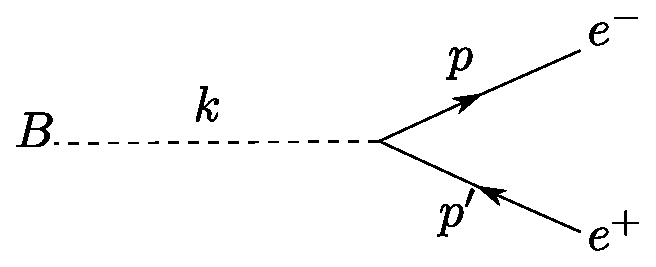
\includegraphics[scale=0.6]{Btoee} %noinstiki
  \caption{Feynman diagrams for $B\to e^+ e^-$} %noinstiki
  \label{fig:btoee} %noinstiki
\end{figure} %noinstiki
Let us define the one--particle states as in eq.~\eqref{eq:38f}

\begin{align}
  | B(\mathbf{p})\rangle\equiv\sqrt{\frac{1}{V}}a^\dagger_{\mathbf{p}}|0\rangle 
\end{align}
From eq.~\eqref{eq:79f} 
\begin{align}
  \label{eq:77f}
   | e^-(\mathbf{p},s)\rangle\equiv&\sqrt{\frac{1}{V}}a^\dagger_s(\mathbf{p})|0\rangle\nonumber\\
   | e^+(\mathbf{p},s)\rangle\equiv&\sqrt{\frac{1}{V}}{b}^\dagger_s(\mathbf{p})|0\rangle\,, 
\end{align}
Using the commutation relations, our states are then normalized as
\begin{align}
\langle B(\mathbf{p})| B(\mathbf{p}')\rangle=&\frac{(2\pi)^3}{V}\delta^3(\mathbf{p}-\mathbf{p}')\nonumber\\
\langle e^-(\mathbf{p},s)| e^-(\mathbf{p}',s')\rangle=&\frac{(2\pi)^3}{V}\delta_{s s'}\delta^3(\mathbf{p}-\mathbf{p}')\nonumber\\
\langle e^+(\mathbf{p},s)| e^+(\mathbf{p}',s')\rangle=&\frac{(2\pi)^3}{V}\delta_{s s'}\delta^3(\mathbf{p}-\mathbf{p}')
\end{align}
As established in Sec.~\ref{sec:fock-space-real}, it is convenient to work in the discrete limit where \eqref{eq:26f}
\begin{align}
   \delta^3(\mathbf{0})=\frac{V}{(2\pi)^3}\,.
\end{align}

Now we can write down the action of various field operators on different one particles states. 
Using the Fourier decomposition  of the scalar field in eq.~\eqref{eq:37f}, and taking into account that 
$a_{\mathbf{p}}|0\rangle=0$, we have
\begin{align}
\label{eq:98f}
   \phi_+(x)|B(\mathbf{k})\rangle=&\int d^3p \frac{1}{(2\pi)^3\sqrt{2\omega_{p} }}
\widehat{a}_{p} e^{-i p\cdot x }
|B(\mathbf{k})\rangle\nonumber\\
=&\int d^3p \frac{1}{(2\pi)^3\sqrt{2\omega_{p}}}
\widehat{a}_\mathbf{p} e^{-i p\cdot x }
\frac{1}{\sqrt{V}}\, \widehat{a}^\dagger_{\mathbf{k}}|0\rangle\nonumber\\
  =&\int d^3p \frac{1}{(2\pi)^3\sqrt{2\omega_{p}V}} e^{-i p\cdot x }
\, [\widehat{a}_{\mathbf{p}},\widehat{a}^\dagger_{\mathbf{k}}]|0\rangle\,.
\end{align}
%check normalization!
By usinbg the commutation relations in eq.~\eqref{eq:32f} we have

\begin{align}
\phi_+(x)|B(\mathbf{k})\rangle  
=&\int d^3p \frac{\delta^{(3)}(\mathbf{p}-\mathbf{k})}{\sqrt{2\omega_{p}V}}
 e^{-i p\cdot x }|0\rangle
\end{align}
\begin{align}
\phi_+(x)|B(\mathbf{k})\rangle  
=&\frac{1}{\sqrt{2\omega_{k}V}}e^{-i k\cdot x }|0\rangle
\end{align}
Similarly, we have


\begin{align}
  \label{eq:99f}
  \phi_+(x)|B(\mathbf{k})\rangle=&\frac{1}{\sqrt{2 \omega_k V}}e^{-i k\cdot x}|0\rangle\nonumber\\
  \psi_+(x)|e^-(\mathbf{p},s)\rangle=&\frac{1}{\sqrt{2 E_p V}}u_s(\mathbf{p})e^{-i p\cdot x}|0\rangle\nonumber\\
  \overline{\psi}_+(x)|e^+(\mathbf{p}',s')\rangle=&\frac{1}{\sqrt{2 E_{p'} V}}\bar{v}_{s'}(\mathbf{p}')e^{-i p'\cdot x}|0\rangle\,,
\end{align}

where $\omega_k$ and $E_p$ represent the energies of the scalar and the electron for the 3-momenta in the subscripts.

Similarly, for the adjoint operators
\begin{align}
  \label{eq:100f}
   \langle B(\mathbf{k})|\phi_-(x)=&\langle0|\frac{1}{\sqrt{2 \omega_k V}}e^{i k\cdot x}\nonumber\\
  \langle e^-(\mathbf{p},s)|\overline{\psi}_-(x)=&\langle0|\frac{1}{\sqrt{2 E_p V}}\bar{u}_s(\mathbf{p})e^{i p\cdot x}\nonumber\\
  \langle e^+(\mathbf{p}',s')|\psi_-(x)=&\langle0|\frac{1}{\sqrt{2 E_{p'} V}}v_{s'}(\mathbf{p}')e^{i p'\cdot x}\,,
\end{align}
In the lowest order the only term which contributes to the matrix element is the term shown in Eq.~\eqref{eq:97f}
The matrix element at first order in Eq.~\eqref{eq:96f}, between the initial and the final state is then
\begin{align}
  S_{fi}^{(1)}=-i h \int d^4x\left\langle e^-(p)e^+(p')\left|\overline{\psi}_-\psi_-\phi_+\right|B(k)\right\rangle\,.
\end{align}
Using Eqs.~\eqref{eq:99f}\eqref{eq:100f}, we obtain
\begin{align}
  S_{fi}^{(1)}=&(-i h)\bar{u}_s(\mathbf{p}) v_{s'}(\mathbf{p}')
\int d^4x\,e^{i(p+p'-k)\cdot x}\frac{1}{\sqrt{2\omega_k V}}\frac{1}{\sqrt{2E_p V}}\frac{1}{\sqrt{2E_{p'} V}}\,.
\end{align}
Since
\begin{align}
  \int d^4x\,e^{i(p+p'-k)\cdot x}=(2\pi)^4\delta^4(k-p-p')\,,
\end{align}
we obtain
\begin{align}
  S_{fi}^{(1)}=&\left[\frac{1}{\sqrt{2\omega_k V}}\frac{1}{\sqrt{2E_p V}}\frac{1}{\sqrt{2E_{p'} V}}\right]
(2\pi)^4\delta^4(k-p-p')\left[(-i h)\bar{u}_s(\mathbf{p}) v_{s'}(\mathbf{p}')\right]
\end{align}
Comparing with Eq.~\eqref{eq:46f} we have therefore that the relativistic matrix element is
\begin{align}
  i\mathcal{M}_{fi}=(-i h)\bar{u}_s(\mathbf{p}) v_{s'}(\mathbf{p}')\,,
\end{align}
and everything else is the history presented in Chapter~\ref{cha:two-body-decays}. 

\section{Wick Theorem}
\label{sec:wick-theorem}
From \cite{Lahiri:2005sm}. The normal ordering procedure involved putting all the annihilation operators to the right of all creation operators so that it annihilates the vacuum. But the time ordering raises complications because in it all operators at earlier times must be further to the right. So creation operators at later times would be to the right of annihilation operators at later times, contrary to what we need for normal ordering. The advantage of normal ordered products is that their expectation values vanish in the vacuum. 

If $H_I$ contains an even number of fermion factors, we can use the time--ordered product $\operatorname{T}\{\ldots\}$ of $n$ factors to write this expression in the equivalent form. For $S^{(2)}$ we have for example
\begin{align}
 \int_{-\infty}^\infty dt_1 \int_{-\infty}^{\infty}d t_2 \operatorname{T}\{H_I(t_2)H_I(t_2)\}=&
\int_{-\infty}^\infty dt_1\int_{-\infty}^{\infty}d t_2 \theta(t_2-t_1)H_I(t_2)H_I(t_2)
+\int_{-\infty}^\infty dt_1\int_{-\infty}^{\infty}d t_2 \theta(t_1-t_2)H_I(t_1)H_I(t_2)
 \end{align}
%%falta el desarrollo
 %\begin{align}
  % \int_{-\infty}^{t_1}d t_2 \theta(t_2-t_1)H_I(t_2)H_I(t_2)+
 %\end{align}
\begin{align}
\int_{-\infty}^\infty dt_1  \int_{-\infty}^{\infty}d t_2 \operatorname{T}\{H_I(t_2)H_I(t_2)\}=&
2\int_{-\infty}^\infty dt_1\int_{-\infty}^{t_1}d t_2 H_I(t_2)H_I(t_2)\,.
 \end{align}


\begin{align}
   S=&1+\sum_{n=1}^\infty\frac{(-i)^n}{n!}\int_{-\infty}^{\infty}d t_1\,\int_{-\infty}^{\infty} d t_2\ldots\int_{-\infty}^{\infty}d t_n\,\operatorname{T}\{{H}_I(t_1){H}_I(t_2)\ldots{H}_I(t_n)\}\,, 
\end{align}
In terms of the Hamiltonian density, we have
\begin{align}
  S=1+\sum_{n=1}^\infty\frac{(-i)^n}{n!}\int\cdots\int d^4x_1 d^4x_2\ldots d^4x_n\,\operatorname{T}\{\mathcal{H}_I(x_1)\mathcal{H}_I(x_2)\ldots\mathcal{H}_I(x_n)\}\,, 
\end{align}
In the above perturbation formalism the states $|i\rangle$ and $|f\rangle$ are, as usual, eigenstates of the unperturbed free-field Hamiltonian $H_0$. As such can be introduced inside the integrals
\begin{align}
  S_{f i}=&\langle f|S|i\rangle\nonumber\\
  =&1+\sum_{n=1}^\infty\frac{(-i)^n}{n!}\int\cdots\int d^4x_1 d^4x_2\ldots d^4x_n\,\langle f|\operatorname{T}\{\mathcal{H}_I(x_1)\mathcal{H}_I(x_2)\ldots\mathcal{H}_I(x_n)\}|i\rangle\,.
\end{align}
For example, at first order
\begin{align}
  \label{eq:96f}
  S_{fi}^{(1)}=&\langle f|S^{(1)}|i\rangle\nonumber\\
  =&\langle f|-i\int d^4x_1\,\operatorname{T}\{\mathcal{H}_I(x_1)\}|i\rangle\nonumber\\
  =&-i\int d^4x_1\,\langle f|:\mathcal{H}_I(x_1):|i\rangle\,.
\end{align}
In order to evaluate this integrals we need to write the time ordered product in terms of the fields. This can done by induction. We start by considering the simple no trivial case with two scalar fields
%ver cuaderno de perrito
\begin{align}
  T\{\phi(x_1)\phi(x_2)\}=:\phi(x_1)\phi(x_2):+\bcontraction{\,}{\phi}{(x_1)}{\phi}
\,\phi(x_1)\phi(x_2)
\end{align}
The same expression can be obtained for fermions. Generalizing  the results for $n$ scalar or fermion fields, but with an even number of fermions fields, we have the Wick theorem
\begin{align}
  T\{\Phi(x_1)\Phi(x_2)\Phi(x_3)\cdots\Phi(x_n) \}
=&:\Phi(x_1)\Phi(x_2)\Phi(x_3)\cdots\Phi(x_n):+\nonumber\\
&+\bcontraction{\,}{\Phi}{(x_1)}{\Phi}\,\Phi(x_1)\Phi(x_2):\Phi(x_3)\cdots\Phi(x_n):\nonumber\\
&+:\Phi(x_1)\bcontraction{\,}{\Phi}{(x_2)}{\Phi}\,\Phi(x_2)\Phi(x_3)\cdots\Phi(x_n):+\cdots 
\end{align}
For details of the full result see for example \cite{Lahiri:2005sm}.


\section{Scattering}
\label{sec:scattering}
From the previous calculation we have
\begin{align}
S^{(n)}=  \frac{(-i)^n}{n!}\int\cdots\int d^4x_1 d^4x_2\ldots d^4x_n\,\operatorname{T}\{\mathcal{H}_I(x_1)\mathcal{H}_I(x_2)\ldots\mathcal{H}_I(x_n)\}\,.
\end{align}
The relevant term for the scattering
\begin{align}
  e^{-}(p_1)+e^{-}(p_2)\to   e^{-}(p_1')+e^{-}(p_2')
\end{align}
is
\begin{align}
S^{(2)}=&  \frac{(-i)^2}{2!}\int\int d^4x_1 d^4x_2\,\operatorname{T}\{\mathcal{H}_I(x_1)\mathcal{H}_I(x_2)\}\nonumber\\
=&  \frac{(-ih)^2}{2!}\int\int d^4x_1 d^4x_2\,\operatorname{T}\{:(\overline{\psi}\psi\phi)_{x_1}(\overline{\psi}\psi\phi)_{x_2}\}\nonumber\\
=& 
 \frac{(-ih)^2}{2!}\int\int d^4x_1 d^4x_2\,:(\overline{\psi}\psi\phi)_{x_1}(\overline{\psi}\psi\phi
)_{x_2}:+
 \frac{(-ih)^2}{2!}\int\int d^4x_1 d^4x_2\,:(\overline{\psi}
\bcontraction{\psi}{\phi}{)_{x_1}(\overline{\psi}\psi}{\phi}
\psi\phi)_{x_1}(\overline{\psi}\psi\phi
)_{x_2}:+\cdots
\end{align}
The first term corresponds to two  disconnected Feynman diagrams that does not contribute to the $S$--matrix. For the process at hand, we want terms where four fermionic operators are not contracted, corresponding to the particles in the initial and final states. The second term in the previous expansion of the Wick theorem is the only satisfying this requirement. In this way
\begin{align}
  S^{(2)}(e^+ e^-\to e^+e^-)=&\frac{(-ih)^2}{2!}\int\int d^4x_1 d^4x_2
\bcontraction{\,}{\phi}{(x_1)}{\phi}
\,\phi(x_1)\phi(x_2):(\overline{\psi}\psi)_{x_1}(\overline{\psi}\psi)_{x_2}:
\end{align}
The Wick contraction can be written as:
\begin{align}
\label{eq:77f}
  \bcontraction{\,}{\phi}{(x_1)}{\phi}
\,\phi(x_1)\phi(x_2)=&\langle0|T\{\phi(x_1)\phi(x_2)\}|0\rangle\nonumber\\
=&i\Delta_F(x_1-x_2)
\end{align}
since
\begin{align}
  \phi(x)=\phi_+(x)+\phi_-(x)\,,
\end{align}
\begin{align}
T\left[\phi(x_1),\phi(x_2)\right]=\theta(t_1-t_2)\phi(x_1)\phi(x_2)+\theta(t_2-t_1)\phi(x_2)\phi(x_1)
\end{align}
\begin{align}
    \langle0|T\left[\phi(x_1),\phi(x_2)\right]|0\rangle=&\theta(t_1-t_2)\langle0|\phi(x_1)\phi(x_2)+\theta(t_2-t_1)\langle0|\phi(x_2)\phi(x_1)|0\rangle\nonumber\\
   =&\theta(t_1-t_2)\langle0|\phi_+(x_1)\phi_-(x_2)+\theta(t_2-t_1)\langle0|\phi_+(x_2)\phi_-(x_1)|0\rangle\nonumber\\
     =&\langle0|\theta(t_1-t_2)\phi(x_1)_+\phi_-(x_2)+\theta(t_2-t_1)\langle0|\phi_+(x_2)\phi_-(x_1)|0\rangle
\end{align}

with
\begin{align}
    \phi_+(x)=&\int d^3p \frac{1}{(2\pi)^3\sqrt{2\omega_{p} }}
\widehat{a}_{p} e^{-i p\cdot x }&
    \phi_-(x)=&\int d^3p \frac{1}{(2\pi)^3\sqrt{2\omega_{p} }}
\widehat{a}_{p}^\dagger e^{i p\cdot x }\,,
\end{align}
we have
\begin{align}
  \langle0|T(\phi(x_1)\phi(x_2))|0\rangle
=&\theta(t_1-t_2)\langle0|\int\frac{d^3p_1}{(2\pi)^3\sqrt{2E_{p_1}}}\hat{a}_{p_1}e^{-i p_1\cdot x_1}
\int\frac{d^3p_2}{(2\pi)^3\sqrt{2E_{p_2}}}\hat{a}_{p_2}^\dagger e^{-i p_2\cdot x_2}|0\rangle\nonumber\\
&+\theta(t_2-t_1)\langle0|\int\frac{d^3p_2}{(2\pi)^3\sqrt{2E_{p_2}}}\hat{a}_{p_2}e^{-i p_2\cdot x_2}
\int\frac{d^3p_1}{(2\pi)^3\sqrt{2E_{p_1}}}\hat{a}_{p_1}^\dagger e^{-i p_1\cdot x_1}|0\rangle\nonumber\\
=&\theta(t_1-t_2)\int\int\frac{d^3p_1d^3p_2}{(2\pi)^6\sqrt{2E_{p_1}}\sqrt{2E_{p_2}}}e^{-i p_1\cdot x_1}e^{-i p_2\cdot x_2}
\langle0|\hat{a}_{p_1}\hat{a}_{p_2}^\dagger|0\rangle\nonumber\\
&+\theta(t_2-t_1)\int\int\frac{d^3p_2d^3p_1}{(2\pi)^6\sqrt{2E_{p_2}}\sqrt{2E_{p_1}}}e^{-i p_2\cdot x_2}e^{-i p_1\cdot x_1}
\langle0|\hat{a}_{p_2}\hat{a}_{p_1}^\dagger|0\rangle\nonumber\\
\end{align}

\begin{align}
=&\theta(t_1-t_2)\int\int\frac{d^3p_1d^3p_2}{(2\pi)^6\sqrt{2E_{p_1}}\sqrt{2E_{p_2}}}e^{-i p_1\cdot x_1}e^{-i p_2\cdot x_2}
\langle0|\hat{a}_{p_1}\hat{a}_{p_2}^\dagger|0\rangle\nonumber\\
&+\theta(t_2-t_1)\int\int\frac{d^3p_2d^3p_1}{(2\pi)^6\sqrt{2E_{p_2}}\sqrt{2E_{p_1}}}e^{-i p_2\cdot x_2}e^{-i p_1\cdot x_1}
\langle0|\hat{a}_{p_2}\hat{a}_{p_1}^\dagger|0\rangle\nonumber\\
\end{align}

On the other hand 
\begin{align}
\label{eq:156f}
  :(\overline{\psi}\psi)_{x_1}(\overline{\psi}\psi)_{x_2}:=&
:\overline{\psi}^\alpha(x_1)\psi^\alpha(x_1)\overline{\psi}^\beta(x_2)\psi^\beta(x_2):\,.
\end{align}

%\left[\right]
%\left(\right)

From the Fourier expansions in eqs.~\eqref{eq:83f}, \eqref{eq:78f} we have that $a_s^\dagger$ and $a_s$ are the creation and annihilation operators for particles. As we have only particles (and not antiparticles) in the initial and final states, the only non-zero contribution of the ordered product in eq.~\eqref{eq:156f} must have the order $a^\dagger a^\dagger a\, a$. As $\psi_+$ and $\overline{\psi}_-$ are associated to $a$ and $a^\dagger$ respectively, the only non-zero contribution from the ordered fermion product is
%\left(\right)

\begin{align}
:(\overline{\psi}\psi)_{x_1}(\overline{\psi}\psi)_{x_2}:  
=-&\overline{\psi}^\alpha_-(x_1)\overline{\psi}^\beta_-(x_2)\psi^\alpha_+(x_1)\psi^\beta_+(x_2)\,.
\end{align}
The relevant $S$--matrix element then reads
\begin{align}
  S^{(2)}_{fi}=&-\frac{(-ih)^2}{2}\int\int d^4x_1 d^4x_2\nonumber\\
&\times\langle e^-(\mathbf{p}_1')e^-(\mathbf{p}_2')|
i\Delta_F(x_1-x_2)\overline{\psi}^\alpha_-(x_1)\overline{\psi}^\beta_-(x_2)\psi^\alpha_+(x_1)\psi^\beta_+(x_2)|e^-(\mathbf{p}_1)e^-(\mathbf{p}_2)\rangle\nonumber\\
=&-\frac{(-ih)^2}{2}\int\int d^4x_1 d^4x_2\,i\Delta_F(x_1-x_2)\nonumber\\
&\times\langle e^-(\mathbf{p}_1')e^-(\mathbf{p}_2')|
\overline{\psi}^\alpha_-(x_1)\overline{\psi}^\beta_-(x_2)\psi^\alpha_+(x_1)\psi^\beta_+(x_2)|e^-(\mathbf{p}_1)e^-(\mathbf{p}_2)\rangle\nonumber\\
=&-\frac{(-ih)^2}{2}\int\int d^4x_1 d^4x_2\int\frac{d^4q}{(2\pi)^4}\,i\Delta_F(q)e^{i q\cdot(x_1-x_2)}\nonumber\\
&\times\langle e^-(\mathbf{p}_1')e^-(\mathbf{p}_2')|
\overline{\psi}^\alpha_-(x_1)\overline{\psi}^\beta_-(x_2)\psi^\alpha_+(x_1)\psi^\beta_+(x_2)|e^-(\mathbf{p}_1)e^-(\mathbf{p}_2)\rangle
\end{align}
The two particle Fock state is, after proper normalization
\begin{align}
  |e^-(\mathbf{p}_1)e^-(\mathbf{p}_2)\rangle=&\frac{1}{\sqrt{V}}a_s^\dagger(\mathbf{p}_2)a_s^\dagger(\mathbf{p}_1)|0\rangle
\end{align}
Therefore
\begin{align}
  \psi^\alpha_+(x_1)\psi^\beta_+(x_2)|e^-(\mathbf{p}_1)e^-(\mathbf{p}_2)\rangle=&
\int\frac{d^3k}{\sqrt{2E_k V}}\int\frac{d^3k}{\sqrt{2E_{k'}V}}
u^\alpha(\mathbf{k})u^\beta(\mathbf{k}')e^{-i k\cdot x_1}e^{-i k'\cdot x_2}\nonumber\\
&\times a_s(\mathbf{k})a_s(\mathbf{k}')a_s^\dagger(\mathbf{p}_2)a_s^\dagger(\mathbf{p}_1)|0\rangle
\end{align}

\begin{align}
  \psi^\alpha_+(x_1)\psi^\beta_+(x_2)|e^-(\mathbf{p}_1)e^-(\mathbf{p}_2)\rangle=&\frac{1}{\sqrt{2E_{p_1} V}}\frac{1}{\sqrt{2E_{p_2}V}}\nonumber\\
&\times\left[u^\alpha(\mathbf{p}_1)u^\beta(\mathbf{p}_2)e^{-i p_1\cdot x_1}e^{-i p_2\cdot x_2}
-u^\alpha(\mathbf{p}_2)u^\beta(\mathbf{p}_1)e^{-i p_2\cdot x_1}e^{-i p_1\cdot x_2}\right]|0\rangle
\end{align}
Following similar steps, we find
\begin{align}
  \langle e^-(\mathbf{p}_1')e^-(\mathbf{p}_2')|
\overline{\psi}^\alpha_-(x_1)\overline{\psi}^\beta_-(x_2)=&
\frac{1}{\sqrt{2E_{p_1}' V}}\frac{1}{\sqrt{2E_{p_2}'V}}\nonumber\\
&\times\langle0|\left[\bar{u}^\alpha(\mathbf{p}_1')\bar{u}^\beta(\mathbf{p}_2')e^{-i p_1'\cdot x_1}e^{-i p_2'\cdot x_2}
-\bar{u}^\alpha(\mathbf{p}_2')u^\beta(\mathbf{p}_1')e^{-i p_2'\cdot x_1}e^{-i p_1'\cdot x_2}\right]
\end{align}
As expected, the final result can be written in term of three different factors: the momentum conservation, normalization, and the relativistic amplitude
\begin{align}
  S^{(2)}_{fi}=i(2\pi)^4\delta^{4}\left(\sum_{i=1,2} p_i-\sum_{f=1,2}p'_f\right)
  \prod_{i=1,2}\frac{1}{\sqrt{2E_i V}}\prod_{f=1,2}\frac{1}{\sqrt{2E_f' V}}\mathcal{M}_{fi}
\end{align}
where
\begin{align}
  \mathcal{M}_{fi}=(ih)^2\left[
\bar{u}^\alpha(\mathbf{p}_2')\bar{u}^\beta(\mathbf{p}_1')\Delta_F(p_1-p_2')u^\alpha(\mathbf{p}_1)u^\beta(\mathbf{p}_2)
-\bar{u}^\alpha(\mathbf{p}_1')\bar{u}^\beta(\mathbf{p}_2')\Delta_F(p_1-p_1')u^\alpha(\mathbf{p}_1)u^\beta(\mathbf{p}_2)
\right]
\end{align}
The two contributions are displayed in Fig.~\ref{fig:sct}
\begin{figure} %noinstiki
  \centering %noinstiki
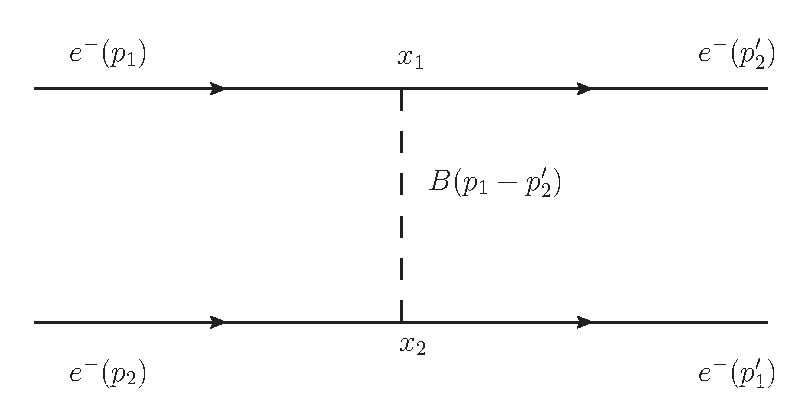
\includegraphics{scattering} %noinstiki
 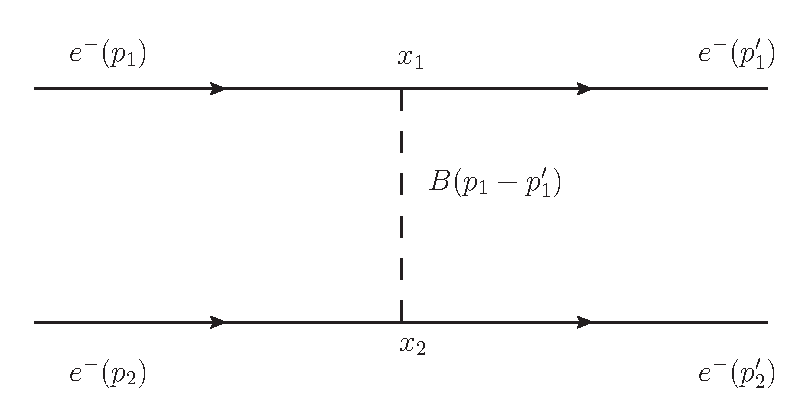
\includegraphics{scattering2} %noinstiki
  \caption{fermion scattering} %noinstiki
  \label{fig:sct} %noinstiki
\end{figure} %noinstiki
Since
\begin{align}
  \Delta_F(q)=\frac{1}{q^2-m^2}
\end{align}
In the limit $q^2\ll m^2$
\begin{align}
  \Delta_F=-\frac{1}{m^2}
\end{align}
\begin{align}
  \mathcal{M}_{fi}=&\frac{h^2}{m^2}\left[
\bar{u}^\alpha(\mathbf{p}_2')u^\alpha(\mathbf{p}_1)\bar{u}^\beta(\mathbf{p}_1')u^\beta(\mathbf{p}_2)
-\bar{u}^\alpha(\mathbf{p}_1')u^\alpha(\mathbf{p}_1)\bar{u}^\beta(\mathbf{p}_2')u^\beta(\mathbf{p}_2)
\right]\nonumber\\
=&\frac{h^2}{m^2}\left[
\bar{u}(\mathbf{p}_2')u(\mathbf{p}_1)\bar{u}(\mathbf{p}_1')u(\mathbf{p}_2)
-\bar{u}(\mathbf{p}_1')u(\mathbf{p}_1)\bar{u}(\mathbf{p}_2')u(\mathbf{p}_2)
\right]
\end{align}
For one interaction of type $\overline{\psi}\Gamma\psi$ we should have
\begin{align}
  \mathcal{M}_{fi}=\frac{h^2}{m^2}\left[
\bar{u}(\mathbf{p}_2')\Gamma u(\mathbf{p}_1)\bar{u}(\mathbf{p}_1')\Gamma u(\mathbf{p}_2)
-\bar{u}(\mathbf{p}_1')\Gamma u(\mathbf{p}_1)\bar{u}(\mathbf{p}_2')\Gamma u(\mathbf{p}_2)
\right]
\end{align}
For the interaction of a fermion pair with $W_\mu^\pm$, we know from
the standard model Lagrangian \cite{lsm}, that
\begin{align}
  \frac{g^2}{2\sqrt{2}}\overline{\psi}\gamma^\mu(1-\gamma_5)\psi
\end{align}
Therefore in this case
\begin{align}
  \Gamma=\gamma^\mu(1-\gamma_5)
\end{align}
For $p\ll M_W^2$ the analysis is similar to the previous one with
\begin{align}
   \bcontraction{\,}{W^\mu}{(x_1)}{W^\nu}
\,W^\mu(x_1)W^\nu(x_2)=&\langle0|T\{W^\mu(x_1)W^\nu(x_2)\}|0\rangle\nonumber\\
\approx&\int\frac{d^4q}{(2\pi)^4}\frac{g^{\mu\nu}}{M_W^2}e^{-i q\cdot(x_1-x_2)}
\end{align}

For the process 
\begin{align}
  e^-(p)+\nu_\mu(k)\to\mu^-(p')+\nu_e(k')
\end{align}
the global coupling for $p\ll M_W^2$ is
\begin{align}
  \frac{g^2}{8M_W^2}=&\frac{G_F}{\sqrt{2}}
\end{align}

After the replacement $G_F/\sqrt{2}\equiv h^2/m^2$, we have
\begin{align}
  \label{eq:101f}
  S^{(2)}_{fi}=i(2\pi)^4\delta^{4}\left(p_1+p_2-p'_1-p'_2\right)
  \frac{1}{\sqrt{2E_1 V}}\frac{1}{\sqrt{2E_2 V}}
  \frac{1}{\sqrt{2E_1' V}}\frac{1}{\sqrt{2E_2' V}}
  \mathcal{M}_{fi}
\end{align}
where
\begin{align}
  \mathcal{M}_{fi}=\frac{G_F}{\sqrt{2}}
\bar{u}_{\nu_e}(\mathbf{p}'_2)\Gamma u_e(\mathbf{p}_1)\bar{u}_\mu(\mathbf{p}'_1)\Gamma u_{\nu_\mu}(\mathbf{p_2})
\end{align}
The corresponding Feynman diagram is shown in Fig.~\ref{fig:sw}
\begin{figure} %noinstiki
  \centering %noinstiki
  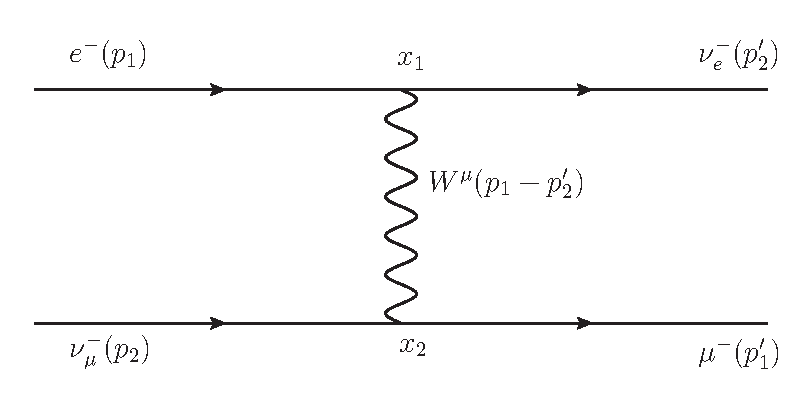
\includegraphics{scatteringw} %noinstiki
  \caption{scattering with four fermions} %noinstiki
  \label{fig:sw} %noinstiki
\end{figure} %noinstiki
Therefore we have

\begin{align}
  \mathcal{M}_{fi}=\frac{G_F}{\sqrt{2}}
\bar{u}_{\nu_e}(\mathbf{p}_2')\gamma^\mu(1-\gamma_5)u_e(\mathbf{p_1})
\bar{u}_\mu(\mathbf{p}_1')\gamma_\mu(1-\gamma_5)u_{\nu_\mu}(\mathbf{p_2})
\end{align}
We now must sqaure the scattering amplitude, $\mathcal{M}$, and summing up over final spin states, and averaging over the intial spin states, as we did in Eq.~\eqref{eq:81f}. The result that will be obtained in detail in Chapter~\ref{cha:three-body-decays} for the muon--decay is
\begin{align}
  \label{eq:102f}
  \overline{|\mathcal{M}|^2}=64\,G_F^2\,(p_1\cdot p_2)(p_1'\cdot p_2')
\end{align}

From Eq.~\eqref{eq:74f}
\begin{align}
  \label{eq:103f}
  \frac{d\sigma}{d\Omega}=\frac{1}{64\pi^2s}\left(\frac{s-m_\mu^2}{s-m_e^2}\right)\overline{|\mathcal{M}|^2}
\end{align}

The center of mass (CM) frame is defined by the condition in Eq.~\eqref{eq:55f}:
\begin{align}
  \mathbf{p}_1+\mathbf{p}_2=0
\end{align}
The $\delta$--function in Eq.~\eqref{eq:101f}
\begin{align}
  \delta^{(4)}(p_1+p_2-p_1'-p_2')=\delta^{(3)}(\mathbf{p}_1+\mathbf{p}_2-\mathbf{p}_1'-\mathbf{p}_2')
\delta(E_1+E_2-E_1'-E_2')
\end{align}

implies
\begin{align}
  \label{eq:157f}
  \mathbf{p}_1+\mathbf{p}_2-\mathbf{p}_1'-\mathbf{p}_2'=0 \overset{\text{CM}}{\Rightarrow}
  \begin{cases}
    \mathbf{p}_1=-\mathbf{p}_2\\
    \mathbf{p}_1'=-\mathbf{p}_2'\\
  \end{cases}
\end{align}
Moreover
\begin{align}
  \sqrt{s}=E_1+E_2
\end{align}
In the CM frame
\begin{align}
\label{eq:104f}
s=&\left(E_1+E_2\right)^2\nonumber\\
=&\left(\sqrt{\mathbf{p}_1^2+m_1^2}+\sqrt{\mathbf{p}_2^2+m_2^2}\right)^2\nonumber\\
=&\left(\sqrt{\mathbf{p}_1^2+m_e^2}+\sqrt{\mathbf{p}_1^2+m_{\nu_e}^2}\right)^2
\end{align}
Therefore
\begin{align}
  \label{eq:105f}
  E_2=|\mathbf{p}_1|
\end{align}
We already have the expression for $|\mathbf{p}_1|$ as given in eq.~\eqref{eq:71f}. In this case $m_2=0$, and $m_1=m_e$, so that
\begin{align}
  \label{eq:158f}
  |\mathbf{p}_1|=\frac{s-m_e^2}{2\sqrt{s}}
\end{align}

From \eqref{eq:105f}
\begin{align}
  \sqrt{s}=&E_1+E_2\nonumber\\
  =&E_1+|\mathbf{p}_1|
\end{align}
\begin{align}
  \label{eq:106f}
  E_1=&\sqrt{s}-|\mathbf{p}_1|\nonumber\\
  =&\sqrt{s}+\frac{-s+m_e^2}{2\sqrt{s}}\nonumber\\
  =&\frac{2s-s+m_e^2}{2\sqrt{s}}\nonumber\\
  =&\frac{s+m_e^2}{2\sqrt{s}}
\end{align}
Then, by using Eqs.~\eqref{eq:157f}, \eqref{eq:105f} and \eqref{eq:158f}, and~\eqref{eq:106f},  we have
\begin{align}
  p_1\cdot p_2=&E_1E_2-\mathbf{p}_1\cdot\mathbf{p}_2\nonumber\\
  =&E_1|\mathbf{p}_1|+\mathbf{p}_1^2\nonumber\\
=&\frac{(s-m_e^2)(s+m_e^2)}{4s}+\frac{(s-m_e^2)^2}{4s}\nonumber\\
=&\frac{(s-m_e^2)}{4s}(s+m_e^2+s-m_e^2)\nonumber\\
=&\frac{1}{2}(s-m_e^2) 
\end{align}
As $p_2^2={p_2'}^2=0$, we have from $\delta$--function
\begin{align}
  (p_1+p_2)^2=&(p_1'+p_2')^2\nonumber\\
  (p_1+p_2)^2=&(p_1'+p_2')^2\nonumber\\
  p_1^2+2p_1\cdot p_2+p_2^2=&{p_1'}^2+2p_1'\cdot p_2'+{p_2'}^2\nonumber\\
  p_1^2+2p_1\cdot p_2=&{p_1'}^2+2p_1'\cdot p_2'\nonumber\\
  m_e^2+2p_1\cdot p_2=&m_\mu^2+2p_1'\cdot p_2'
\end{align}
\begin{align}
  p_1'\cdot p_2'=p_1\cdot p_2-\frac{1}{2}(m_\mu^2-m_e^2)
\end{align}
\begin{align}
  p_1'\cdot p_2'=\frac{1}{2}(s-m_\mu^2) 
\end{align}
Replacing back in Eq.~\eqref{eq:102f} and then in Eq.~\eqref{eq:103f} we have
\begin{align}
  \frac{d\sigma}{d\Omega}=\frac{1}{64\pi^2s}\left(\frac{s-m_\mu^2}{s-m_e^2}\right)
64G_F^2\frac{1}{2}(s-m_e^2)\frac{1}{2}(s-m_\mu^2)
\end{align} 
\begin{align}
    \frac{d\sigma}{d\Omega}=\frac{G_F^2}{4\pi^2}\frac{(s-m_\mu^2)^2}{s}
\end{align}
\begin{align}
\sigma  =\frac{G_F^2}{\pi}\frac{(s-m_\mu^2)^2}{s}
\end{align}
Note that $\sigma\propto s$.
%\left(\right)
%\left[\right]


%%% Local Variables: 
%%% mode: latex
%%% TeX-master: "beyond"
%%% End: 


%instiki:category: QuantumFieldTheory
\chapter{Three body decays}
\label{cha:three-body-decays} %noinstiki
%instiki:
%instiki:***
%instiki:
%instiki:[[Beyond|Contents]]
%instiki:
%instiki:***
%instiki:
%instiki:* [Muon decay](#mu-decay)
%instiki: 
%instiki:* [three body decays in radiative seesaw](#three-body-decays)
%instiki:
%instiki:* [Sample point](#sample-point)
%instiki:
%instiki:* [Preliminary discussion](#prel-disc)
%instiki:

\section{Muon decay}
\label{sec:mu-decay} 

For a three body decay we have from eq.~\eqref{eq:76}
\begin{align}
  \label{eq:107}
  d\Gamma =& \frac{1}{(2\pi)^5}\frac{1}{2M}\left|\mathcal{M}\right|^2 \delta^4(P-p_1-p_2-p_3)\frac{d^3 p_1}{2E_1}
\frac{d^3 p_2}{2E_2}\frac{d^3 p_3}{2E_3}\nonumber\\
  =& \frac{1}{(2\pi)^5}\frac{1}{2M}\frac{d^3 p_1}{2E_1}\int\left|\mathcal{M}\right|^2 \delta^4(P-p_1-p_2-p_3)
\frac{d^3 p_2}{2E_2}\frac{d^3 p_3}{2E_3}\nonumber\\
\end{align}

\subsection{Amplitude estimation}
\label{sec:amplitude-estimation}
Since $\mathcal{M}$ is dimensionless, the amplitude averaged over spins for $\mu$ decay must be
\begin{equation}
  |\mathcal{M}|^2=C G_F^2 m_\mu^4\,.
\end{equation}
We use
\begin{equation}
  C=\frac{1}{2}(2\times2\times1\times1)=2
\end{equation}
The first factor is for the initial average and the factor are for the number of spin states of $\mu$, $e$ and the two neutrinos. 


Consider first the integral
\begin{align}
  \int \delta^4(P-p_1-p_2)
\frac{d^3 p_1}{2E_1}\frac{d^3 p_2}{2E_2}=&\int\delta(E-E_1-E_2)
\delta^3(\mathbf{P}-\mathbf{p}_1-\mathbf{p}_2)\frac{d^3 p_1}{2E_1}\frac{d^3 p_2}{2E_2}\nonumber\\
  =&\int\delta(E-E_1-E_2)
\frac{d^3 p_2}{4E_1 E_2}\int\delta^3(\mathbf{P}-\mathbf{p}_1-\mathbf{p}_2){d^3 p_1}\nonumber\\
  =&\int\delta(E-E_1-E_2)
\frac{d^3 p_2}{4E_1 E_2}\int\delta^3(\mathbf{p}_1+\mathbf{p}_2-\mathbf{P}){d^3 p_1}\nonumber\\
  =&\int\delta(E-E_1-E_2)
\frac{d^3 p_2}{4E_1 E_2}\int\delta^3[\mathbf{p}_1-(\mathbf{P}-\mathbf{p}_2)]{d^3 p_1}
\end{align}
using
\begin{align}
  \int\delta(x-x_0)dx=1
\end{align}
we have
\begin{align}
  \label{eq:108}
    \int \delta^4(P-p_1-p_2)
\frac{d^3 p_1}{2E_1}\frac{d^3 p_2}{2E_2}=&
\int\delta(E-E_1-E_2)\frac{d^3 p_2}{4E_1 E_2}\nonumber\\
    \int \delta^4(P-p_1-p_2)
\frac{d^3 p_1}{2E_1}\frac{d^3 p_2}{2E_2}=&
\int\delta(E-E_1-E_2)\frac{\mathbf{p}_2^2\,d|\mathbf{p}_2|d\Omega}{4E_1 E_2}
\end{align}
Since $|\mathbf{p}_1|=|\mathbf{p}_2|$ we have
\begin{align}
  E=E_1+E_2=&(m_1^2+\mathbf{p}_1^2)^{1/2}+(m_2^2+\mathbf{p}_2^2)^{1/2}\nonumber\\
  =&(m_1^2+\mathbf{p}_2^2)^{1/2}+(m_2^2+\mathbf{p}_2^2)^{1/2}
\end{align}
differentiating this equation with respect to $\mathbf{p}_2$
\begin{align}
  \frac{d E}{d|\mathbf{p}_2|}=&\frac{1}{2}\left(
\frac{2|\mathbf{p}_2|}{(m_1^2+\mathbf{p}_2^2)^{1/2}}+
\frac{2|\mathbf{p}_2|}{(m_2^2+\mathbf{p}_2^2)^{1/2}}\right)\nonumber\\
=&|\mathbf{p}_2|\left(\frac{1}{E_1}+\frac{1}{E_2}\right)\nonumber\\
  =&|\mathbf{p}_2|\left(\frac{E_1+E_2}{E_1 E_2}\right)
\end{align} 
Therefore
\begin{align}
  d|\mathbf{p}_2|=\frac{d E}{|\mathbf{p}_2|}\left(\frac{E_1 E_2}{E_1+E_2}\right)
\end{align}
replacing back in eq.~(\ref{eq:108})
\begin{align}
      \int \delta^4(P-p_1-p_2)\frac{d^3 p_1}{2E_1}\frac{d^3 p_2}{2E_2}
      =&\int\frac{d E}{|\mathbf{p}_2|}\,\delta(E-E_1-E_2)\frac{\mathbf{p}_2^2\,d\Omega}{4E_1 E_2}
      \left(\frac{E_1 E_2}{E_1+E_2}\right)\nonumber\\
      =&\int d E\,\delta(E-E_1-E_2)\frac{|\mathbf{p}_2|\,d\Omega}{4(E_1+E_2)}\nonumber\\
      =&  \int\frac{|\mathbf{p}_2|}{4 E}d\Omega
\end{align}
For a relativistic particle $|\mathbf{p}_2|\approx E_2=E/2$ and
\begin{align}
  \int \delta^4(P-p_1-p_2)\frac{d^3 p_1}{E_1}\frac{d^3 p_2}{E_2}=2\pi
\end{align}
Applying this result to eq.~(\ref{eq:107}) we have
\begin{align}
    d\Gamma =& \frac{1}{(2\pi)^5}\frac{1}{2M}\frac{d^3 p_1}{2E_1}\int\left|\mathcal{M}\right|^2 \delta^4(P-p_1-p_2-p_3)
\frac{d^3 p_2}{2E_2}\frac{d^3 p_3}{2E_3}\nonumber\\
=&\frac{1}{(2\pi)^5}\frac{1}{2M}\frac{d^3 p_1}{8E_1}\left|\mathcal{M}\right|^2\int \delta^4(P-p_1-p_2-p_3)
\frac{d^3 p_2}{E_2}\frac{d^3 p_3}{E_3}\nonumber\\
=&\frac{1}{(2\pi)^5}\frac{1}{2M}\frac{d^3 p_1}{8E_1}\left|\mathcal{M}\right|^2(2\pi)\nonumber\\
  =&\frac{G_F^2m_\mu^4}{8(2\pi)^4 m_\mu E_1} \mathbf{p}_1^2 d|\mathbf{p}_1|\int d\Omega\nonumber\\
  \approx&\frac{G_F^2m_\mu^3}{8(2\pi)^4  E_1} E_1^2 d E_1(4\pi)\nonumber\\
  \approx&\frac{G_F^2m_\mu^3}{4(2\pi)^3} E_1 d E_1
\end{align}
As the maximum value  of $E_1$ is $m_\mu/2$
\begin{align}
  \Gamma\approx&\frac{G_F^2m_\mu^3}{4(2\pi)^3} \int_0^{m_\mu/2}E_1 d E_1\nonumber\\
   =&\frac{G_F^2m_\mu^3}{4(2\pi)^3} \frac{m_\mu^2}{8}\,,
\end{align}
or
\begin{equation}
  \Gamma=\frac{3}{4}\frac{G_F^2m_\mu^5}{192\pi^3}\,.
\end{equation}

\subsection{Amplitude calculation}
\label{sec:ampl-calc}
The Standard Model Lagrangian includes
\begin{align}
  \mathcal{L}=&-\frac{\sqrt{2}g}{2}(\overline{\nu_e}_L\gamma^\mu e_L W_\mu^++\bar{e}_L\gamma^\mu{\nu_e}_L W_\mu^-+\overline{\nu_\mu}_L\gamma^\mu\mu_L W_\mu^++\bar{\mu}_L\gamma^\mu{\nu_\mu}_L W_\mu^-)\nonumber\\
=&-\frac{g}{\sqrt{2}}(\overline{\nu_e}\gamma^\mu P_L e W_\mu^++\bar{e}\gamma^\mu P_L{\nu_e} W_\mu^-+\overline{\nu_\mu}\gamma^\mu P_L\mu W_\mu^++\bar{\mu}\gamma^\mu P_L{\nu_\mu} W_\mu^-)\nonumber\\
=&-\frac{g}{2\sqrt{2}}(\overline{\nu_e}\gamma^\mu (1-\gamma_5) e W_\mu^++\bar{e}\gamma^\mu (1-\gamma_5){\nu_e} W_\mu^-+\overline{\nu_\mu}\gamma^\mu (1-\gamma_5)\mu W_\mu^++\bar{\mu}\gamma^\mu (1-\gamma_5){\nu_\mu} W_\mu^-)
\end{align}
where
\begin{align}
  \label{eq:109}
  (\overline{\nu_e}\gamma^\mu P_L e W_\mu^+)^\dagger&=e^\dagger{\gamma^\mu P_L}^\dagger(\overline{\nu_e})^\dagger W_\mu^-
  =e^\dagger P_L{\gamma^\mu}^\dagger\gamma^0\nu_e W_\mu^-=e^\dagger\gamma^0\gamma^0{\gamma^\mu}^\dagger P_R\gamma^0\nu_e W_\mu^-\nonumber\\
  &=\bar{e}\gamma^0{\gamma^\mu}^\dagger\gamma^0P_L\nu_e W_\mu^-=\bar{e}\gamma^\mu P_L\nu_e W_\mu^-
\end{align}
We can build the effective Lagrangian

Applying the Feynman rules to the diagram in fig. 
\ref{fig:1} %noinstiki
we have the amplitude
\begin{align}
  \mathcal{M}=\frac{-ig^2}{8}\bar{u}_3\gamma_\mu(1-\gamma_5)u_1\left(\frac{-g^{\mu\nu}+q^\mu q^\nu/M_W^2}{q^2-M_W^2}\right)\bar{u}_4\gamma_\nu(1-\gamma_5)v_2
\end{align}
where $u$ ($v$) is for an incoming particle and $\bar{u}$ ($\bar{v}$) is for an ongoing particle (antiparticle).

\begin{figure} %noinstiki
  \centering %noinstiki
  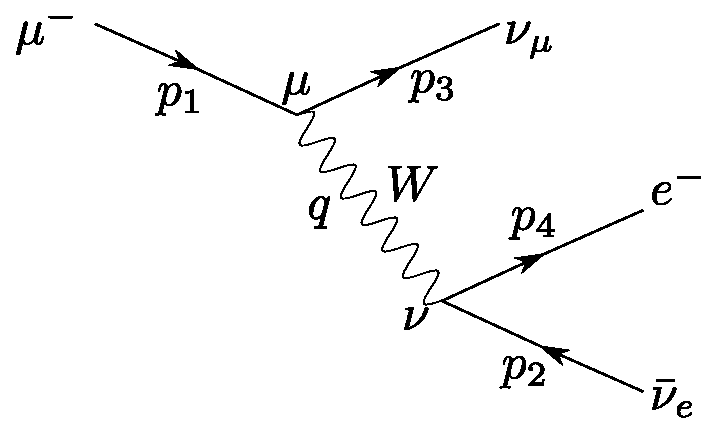
\includegraphics{muon_decay}%noinstiki
  \caption{Tree level diagram for muon decay } %noinstiki
  \label{fig:1} %noinstiki
\end{figure} %noinstiki


The Dirac equations for spinors $u$ and $v$ are
\begin{align}
  (\cancel{p}-m)u&=0&(\cancel{p}+m )v&=0\nonumber\\
  \bar{u}(\cancel{p}-m)&=0&\bar{v}(\cancel{p}+m )&=0\,.
\end{align}
In this way
\begin{align}
  \frac{1}{M_W^2}\gamma_\mu q^\mu(1-\gamma_5)u_1 \bar{u}_4\gamma_\nu q^\nu(1-\gamma_5)
  =&\frac{1}{M_W^2}(1+\gamma_5)\cancel{q}u_1 \bar{u}_4\cancel{q}(1-\gamma_5)\nonumber\\
  =&-\frac{m_\mu m_e}{M_W^2}(1+\gamma_5)u_1 \bar{u}_4(1-\gamma_5)\,
\end{align}
the term in $q^\mu q^\nu$ can be safely neglected. The term $q^2$ is $m_\mu^2$ is small compared with $m_W^2$. Therefore
\begin{align}
  \mathcal{M}=&\frac{-i g^2}{8M_W^2}\bar{u}_3\gamma_\mu(1-\gamma_5)u_1\bar{u}_4\gamma^\mu(1-\gamma_5)v_2\nonumber\\
  =&\frac{-i G_F}{\sqrt{2}}\bar{u}_3\gamma_\mu(1-\gamma_5)u_1\bar{u}_4\gamma^\mu(1-\gamma_5)v_2
\end{align}
$\mathcal{M}$ is a dimensionless scalar. The relevant coupling is
\begin{equation}
  \frac{g^2}{8M_W^2}=\frac{G_F}{\sqrt{2}}\,.
\end{equation}
The conjugate is, following  the same steps that in eq.~\eqref{eq:109}
\begin{align}
  \mathcal{M}^*=&\frac{i g^2}{8M_W^2}\left[\bar{u}_3\gamma_\mu(1-\gamma_5)u_1\right]^\dagger
  \left[\bar{u}_4\gamma^\mu(1-\gamma_5)v_2\right]^\dagger\nonumber\\
   \mathcal{M}^*=&\frac{i g^2}{8M_W^2}\left[\bar{u}_1\gamma_\mu(1-\gamma_5)u_3\right]
  \left[\bar{v}_2\gamma^\mu(1-\gamma_5)u_4\right]\,.
\end{align}
Multiplying $\mathcal{M}$ and $\mathcal{M}^*$ we have
\begin{align}
  \label{eq:110}
  |\mathcal{M}|^2=&\frac{g^4}{64 M_W^4}\left[\bar{u}_3\gamma_\mu(1-\gamma_5)u_1\bar{u}_1\gamma_\nu(1-\gamma_5)u_3\right]\nonumber\\
  &\times\left[\bar{u}_4\gamma^\mu(1-\gamma_5)v_2\bar{v}_2\gamma^\nu(1-\gamma_5)u_4\right]\nonumber\\
  =&\frac{g^4}{64 M_W^4}L_{\mu\nu}M^{\mu\nu}
\end{align}
where
\begin{align}
   L_{\mu\nu}=&\left[\bar{u}_{3\alpha}\gamma_\mu^{\alpha\beta}(1-\gamma_5)_{\beta\gamma}u_1^\gamma\bar{u}_{1\delta}\gamma_\nu^{\delta\epsilon}(1-\gamma_5)_{\epsilon\eta}u_3^\eta\right]\nonumber\\
  M^{\mu\nu}=&\left[\bar{u}_4^\alpha\gamma^\mu_{\alpha\beta}(1-\gamma_5)^{\beta\gamma}v_{2\gamma}\bar{v}_2^\delta\gamma^\nu_{\delta\epsilon}(1-\gamma_5)^{\epsilon\eta}u_{4\eta}\right]
\end{align}
\begin{align}
     L_{\mu\nu}=&\left[u_3^\eta\bar{u}_{3\alpha}\gamma_\mu^{\alpha\beta}(1-\gamma_5)_{\beta\gamma}u_1^\gamma\bar{u}_{1\delta}\gamma_\nu^{\delta\epsilon}(1-\gamma_5)_{\epsilon\eta}\right]\nonumber\\
     =&\left[(u_3\bar{u}_{3})_{\eta\alpha}\gamma_\mu^{\alpha\beta}(1-\gamma_5)_{\beta\gamma}(u_1\bar{u}_{1})_{\gamma\delta}\gamma_\nu^{\delta\epsilon}(1-\gamma_5)_{\epsilon\eta}\right]\nonumber\\
     =&\operatorname{Tr}\left[(u_3\bar{u}_{3})\gamma_\mu(1-\gamma_5)(u_1\bar{u}_{1})\gamma_\nu(1-\gamma_5)\right]
\end{align}
Using
\begin{align}
  \label{eq:111}
 \sum_su(p,s)\bar{u}(p,s)&=(\cancel{p}+m)& \sum_sv(p,s)\bar{v}(p,s)&=(\cancel{p}-m)
\end{align}
\begin{align}
  \sum_s L_{\mu\nu}=&\operatorname{Tr}\left[(\cancel{p}_3)\gamma_\mu(1-\gamma_5)(\cancel{p}_1+m_\mu)\gamma_\nu(1-\gamma_5)\right]\nonumber\\
  =&p_3^\alpha\operatorname{Tr}\left[\gamma_\alpha\gamma_\mu(1-\gamma_5)(p_1^\beta\gamma_\beta+m_\mu)\gamma_\nu(1-\gamma_5)\right]\nonumber\\
  =&p_3^\alpha\operatorname{Tr}\left[(\gamma_\alpha\gamma_\mu-\gamma_\alpha\gamma_\mu\gamma_5)(p_1^\beta\gamma_\beta\gamma_\nu(1-\gamma_5)+m_\mu\gamma_\nu(1-\gamma_5))\right]\nonumber\\
  =&p_3^\alpha\operatorname{Tr}\left[p_1^\beta\gamma_\alpha\gamma_\mu\gamma_\beta\gamma_\nu(1-\gamma_5)-p_1^\beta\gamma_\alpha\gamma_\mu\gamma_5\gamma_\beta\gamma_\nu(1-\gamma_5)\right.\nonumber\\
&\left.+m_\mu\gamma_\alpha\gamma_\mu\gamma_\nu(1-\gamma_5)-m_\mu\gamma_\alpha\gamma_\mu\gamma_5\gamma_\nu(1-\gamma_5)\right]\nonumber\\
  =&p_3^\alpha\operatorname{Tr}\left[p_1^\beta\gamma_\alpha\gamma_\mu\gamma_\beta\gamma_\nu-p_1^\beta\gamma_\alpha\gamma_\mu\gamma_\beta\gamma_\nu\gamma_5-p_1^\beta\gamma_\alpha\gamma_\mu\gamma_5\gamma_\beta\gamma_\nu
+p_1^\beta\gamma_\alpha\gamma_\mu\gamma_5\gamma_\beta\gamma_\nu\gamma_5\right.\nonumber\\
&\left.+m_\mu\gamma_\alpha\gamma_\mu\gamma_\nu-m_\mu\gamma_\alpha\gamma_\mu\gamma_\nu\gamma_5-m_\mu\gamma_\alpha\gamma_\mu\gamma_5\gamma_\nu+m_\mu\gamma_\alpha\gamma_\mu\gamma_5\gamma_\nu\gamma_5\right]
\end{align}
as the trace of an odd number of $\gamma$--matrices is zero, we have
\begin{align}
  \sum_s L_{\mu\nu}=&p_3^\alpha p_1^\beta\operatorname{Tr}\left[\gamma_\alpha\gamma_\mu\gamma_\beta\gamma_\nu-\gamma_\alpha\gamma_\mu\gamma_\beta\gamma_\nu\gamma_5-\gamma_\alpha\gamma_\mu\gamma_\beta\gamma_\nu\gamma_5
+\gamma_\alpha\gamma_\mu\gamma_\beta\gamma_\nu\gamma_5^2\right]\nonumber\\
=&2 p_3^\alpha p_1^\beta\operatorname{Tr}\left[\gamma_\alpha\gamma_\mu\gamma_\beta\gamma_\nu(1-\gamma_5)\right]
\end{align}
Similarly
\begin{align}
  \sum_s M^{\mu\nu}=2 p_{4\delta}p_{2\epsilon}\operatorname{Tr}\left[\gamma^\delta\gamma^\mu\gamma^\epsilon\gamma^\nu(1-\gamma_5)\right]
\end{align}
substituting back in eq.~(\ref{eq:110}) we have,
\begin{align}
  \label{eq:112}
   |\mathcal{M}|^2=&\frac{g^4}{64 M_W^4}4p_3^\alpha p_1^\beta p_{4\delta}p_{2\epsilon}
   \operatorname{Tr}\left[\gamma_\alpha\gamma_\mu\gamma_\beta\gamma_\nu(1-\gamma_5)\right]
   \operatorname{Tr}\left[\gamma^\delta\gamma^\mu\gamma^\epsilon\gamma^\nu(1-\gamma_5)\right]\nonumber\\
   =&\frac{g^4}{64 M_W^4}4p_3^\alpha p_1^\beta p_{4\delta}p_{2\epsilon}(64\delta^\alpha_\delta\delta^\beta_\epsilon)\nonumber\\
  =&\frac{g^4}{64 M_W^4}4\times64(p_3\cdot p_4)(p_1\cdot p_2)\nonumber\\
  =&\frac{4g^4}{M_W^4}(p_3\cdot p_4)(p_1\cdot p_2)\nonumber\\
  =&4\left(8\frac{g^2}{8M_W^2}\right)^2(p_3\cdot p_4)(p_1\cdot p_2)\nonumber\\
  =&4\left(8\frac{G_F}{\sqrt{2}}\right)^2(p_3\cdot p_4)(p_1\cdot p_2)\nonumber\\
  =&128\, G_F^2(p_3\cdot p_4)(p_1\cdot p_2)\nonumber\\
  =&256\frac{G_F^2}{{2}}(p_3\cdot p_4)(p_1\cdot p_2)\,.
\end{align}
The demonstration of the used Tr$\times$Tr identity can be found in Appendix B. of \cite{PeterRenton}.

The spin--averaged differential decay width for $\mu^-\to\nu_\mu e^-\bar{\nu}_e$ is
\begin{align}
  \label{eq:113}
  d\Gamma =& \frac{1}{(2\pi)^5}\frac{1}{2E_1}\frac{d^3 p_3}{2E_3}
\left(\frac{1}{2}\sum\left|\mathcal{M}\right|^2\right) \delta^4(p_1-p_2-p_3-p_4)
\frac{d^3 p_2}{2E_2}\frac{d^3 p_4}{2E_4}\nonumber\\
 =&\frac{1}{2E_1}\frac{1}{2}\sum\left|\mathcal{M}\right|^2\frac{1}{(2\pi)^5}\frac{d^3 p_2}{8E_2}
  \delta^4(p_1-p_2-p_3-p_4)\frac{d^3 p_3}{E_3}\frac{d^3 p_4}{E_4}\nonumber\\
=&\frac{1}{2}\frac{4g^4}{M_W^4}\frac{1}{(2\pi)^52E_1}(p_1\cdot p_2)(p_3\cdot p_4)\frac{d^3 p_2}{2E_2}
  \delta^4(p_1-p_2-p_3-p_4)\frac{d^3 p_3}{2E_3}\frac{d^3 p_4}{2E_4}\nonumber\\
  =&\frac{2g^4}{16 (2\pi)^5 M_W^4 E_1 E_4}p_1^\beta p_4^\alpha d^3p_4 I_{\alpha\beta}
\end{align}
where the covariant integral $I_{\alpha\beta}$ on the neutrino momentum is
\begin{align}
  \label{eq:114}
  I_{\alpha\beta}=\int p_{3\alpha}p_{2\beta}\delta^4(p-p_2-p_3)\frac{d^3 p_2}{E_2}\frac{d^3 p_3}{E_3}\,.
\end{align}
The variable $p$ in ec.~\eqref{eq:114} is defined as $p=p_1-p_4=p_2+p_3$. Moreover
\begin{align}
  \label{eq:115}
  p^2=&p_2^2+p_3^2+2p_2\cdot p_3\nonumber\\
  =&m_{\nu_e}^2+m_{\nu_\mu}^2+2p_2\cdot p_3\nonumber\\
  \approx&2p_2\cdot p_3\nonumber\\
g_{\alpha\beta}p^\alpha p^\beta=&2 g_{\alpha\beta}p_3^\alpha p_2^\beta\nonumber\\
p^\alpha p^\beta=&2p_3^\alpha p_2^\beta\,.
\end{align}
$I_{\alpha\beta}$ must have the form
\begin{align}
  \label{eq:116}
  I_{\alpha\beta}=g_{\alpha\beta}A(p^2)+p_\alpha p_\beta B(p^2)\,.
\end{align}
Defining the itegral $I$ as follows
\begin{equation}
  I=\int\delta^4(p-p_2-p_3)\frac{d^3 p_2}{E_2}\frac{d^3 p_3}{E_3}\,,
\end{equation}
Since
\begin{align}
  m_\nu^2\approx0=&E_\nu^2-\mathbf{p}_\nu^2\nonumber\\
E_\nu^2=&\mathbf{p}_\nu^2
\end{align}
and in addition the integral $I$ is covariant, we choose to evaluate it in the rest frame of the two neutrinos
$|\mathbf{p}_2|=|\mathbf{p}_3|$, which implies $E_2=E_3$.
\begin{align}
  I=&\int\delta(E-E_2-E_3)\delta^3(\mathbf{p}-\mathbf{p}_2-\mathbf{p}_3)\frac{d^3 p_2}{E_2}\frac{d^3 p_3}{E_3}\nonumber\\
    =&\int\delta(E-E_2-E_3)\frac{d^3 p_2}{E_2E_3}\underbrace{\int\delta^3(\mathbf{p}-\mathbf{p}_2-\mathbf{p}_3)d^3 p_3}_{=1}\nonumber\\
    =&\int\frac{\delta(E-2E_2)}{E_2^2}\mathbf{p}_2^2 d|\mathbf{p}_2|d\Omega\nonumber\\
    =&\int\frac{\delta(E-2E_2)}{E_2^2}E_2^2 dE_2 (4\pi)\nonumber\\
    =&4\pi\int\delta\left(2\left(E_2-\frac{E}{2}\right)\right) dE_2 \nonumber\\
    =&4\pi\frac{1}{2}\int\delta\left(E_2-\frac{E}{2}\right) dE_2 \nonumber\\
    =&2\pi
\end{align}

then multiplying (6.13) by $g^{\alpha\beta}$ and $p^\alpha p^\beta$ successively gives, using eq.~\eqref{eq:115}
\begin{equation}
  g^{\alpha\beta}I_{\alpha\beta}=4 A +p^2 B=\int p_{3}\cdot
  p_{2}\delta^4(p-p_2-p_3)\frac{d^3 p_2}{E_2}\frac{d^3
    p_3}{E_3}\nonumber =\frac{p^2}{2}I=\pi p^2\nonumber
\end{equation}

In order to compute $p^\alpha p^\beta I_{\alpha\beta}$, we make use of
the fact that it is a Lorentz invariant quantity, so that we may
evaluate it in any reference frame. In particular, we can evaluate it
in the rest frame of the neutrinos involved in this process. This
means that $p=p_2+p_3=(p^0,\mathbf{0})$ and $E_2=E_3$
\begin{align}
p^\alpha p^\beta I_{\alpha\beta}&=p^2 A+p^4 B\\ 
&=p^\alpha
p^\beta\int\frac{d^3 p_2}{E_2}\frac{d^3 p_3}{E_3}
p_{3\alpha}p_{2\beta}\delta^4(p-p_2-p_3) \nonumber\\
&=\int \frac{d^3
  p_2}{E_2}\frac{d^3 p_3}{E_3} E_3p^0E_2p^0\delta^4(p-p_2-p_3)\nonumber\\
&=(p^0)^2\int d^3 p_2d^3 p_3
\delta^4(p-p_2-p_3)\\
&=(p^0)^2\int d^3 p_2 \delta(p^0-2E_2)\nonumber\\
&=(p)^2\int d E_2 E_2^2 d\Omega
\frac{1}{2}\delta(\frac{p^0}{2}-E_2) 
=4\pi\frac{p^2}{2}\left(\frac{p^2}{2}\right)^2 \nonumber\\
&=\frac{\pi p^4}{2}
\end{align}
where the usual tricks have been used to simplify the integrals, using
the delta function inside.

Therefore
\begin{equation}
  A=\frac{p^2}{4}(\pi-B)
\end{equation}
\begin{align}
  \frac{p^4}{4}(\pi-B)+p^4B=&\frac{\pi p^4}{2}\nonumber\\
    \frac{\pi}{4} -\frac{B}{4}+B=&\frac{\pi}{2}\nonumber\\
    \frac{3B}{4}=&\frac{\pi}{4}\nonumber\\
    B=&\frac{\pi}{3}
\end{align}
\begin{align}
  A=&\frac{p^2}{4}(\pi-\frac{\pi}{3})\nonumber\\
  =&\frac{p^2}{4}(\frac{2\pi}{3})\nonumber\\
  =&\frac{\pi p^2}{6}
\end{align}
\begin{align}
  I_{\alpha\beta}=\frac{\pi}{6}\left(g_{\alpha\beta}p^2+2p_\alpha p_\beta  \right)\,.
\end{align}
Substituting back in eq.~(\ref{eq:113}) we have 
\begin{align}
  \label{eq:117}
  d\Gamma =& \frac{2\pi g^4}{16\times6 (2\pi)^5 M_W^4 E_1 E_4}p_1^\beta p_4^\alpha (g_{\alpha\beta}p^2+2p_\alpha p_\beta)d^3p_4 \nonumber\\
  d\Gamma =& \frac{2g^4}{16\times12 (2\pi)^4 M_W^4 E_1 E_4}[(p_1\cdot p_4)p^2+2(p\cdot p_1)(p\cdot p_4)]d^3p_4 \nonumber\\
  d\Gamma =& \frac{2g^4}{192 (2\pi)^4 M_W^4 E_1 E_4}[(p_1\cdot p_4)p^2+2(p\cdot p_1)(p\cdot p_4)]d^3p_4 
\end{align}
For further evaluation we will use the rest frame of the decaying muon. In this frame the four--momentum are
\begin{align}
  p_1=&(m_\mu,\mathbf{0})\nonumber\\
  p_4=&(E_4,\mathbf{p}_4)\nonumber\\
  p=&p_1-p_4=(m_\mu-E_4,-\mathbf{p}_4)\nonumber\\
  p^2=&E^2-\mathbf{p}^2=m_\mu^2-2m_\mu E_4+(E_4^2-\mathbf{p}_4^2)=m_\mu^2+m_e^2-2m_\mu E_4
\end{align}
Moreover
\begin{align}
  \label{eq:118}
  p_1\cdot p_4=&m_\mu E_4\nonumber\\
  p\cdot p_1=&m_\mu^2-m_\mu E_4\nonumber\\
  p\cdot p_4=&m_\mu E_4-E_4^2+\mathbf{p}_4^2=m_\mu E_4-m_e^2\nonumber\\
  p_4^2=m_e^2&=E_4^2-\mathbf{p}_4^2\Rightarrow\mathbf{p}_4^2=E_4^2-m_e^2\nonumber\\
  |\mathbf{p}_4| =&(E_4^2-m_e^2)^{1/2}\nonumber\\
  &\Rightarrow\frac{d|\mathbf{p}_4|}{d E_4}=\frac{1}{2}\frac{2E_4}{(E_4^2-m_e^2)^{1/2}}=\frac{E_4}{|\mathbf{p}_4|}\nonumber\\
  &\Rightarrow d|\mathbf{p}_4|=\frac{E_4}{|\mathbf{p}_4|} d E_4\nonumber\\
  d^3p_4=&\mathbf{p}_4^2 \,d |\mathbf{p}_4|\,d\Omega=|\mathbf{p}_4|E_4\,d E_4\, d\Omega
\end{align}
Substituting back in eq.~(\ref{eq:117}) we have 
\begin{align}
  d\Gamma=&\frac{2g^4}{192 (2\pi)^4 M_W^4 m_\mu }|\mathbf{p}_4|\,d E_4\,d\Omega[(m_\mu^2+m_e^2-2m_\mu E_4)m_\mu E_4 
  +2(m_\mu^2-m_\mu E_4)(m_\mu E_4-m_e^2)]
\end{align}
Neglecting electron mass we have $|\mathbf{p}_4| = E_4$, and
\begin{align}
  \label{eq:159}
   d\Gamma=&\frac{2g^4(4\pi)}{192 (2\pi)^4 M_W^4 m_\mu }E_4\,d E_4[(m_\mu^2-2m_\mu E_4)m_\mu E_4 
  +2(m_\mu^2-m_\mu E_4)m_\mu E_4]\nonumber\\
  =&\frac{2\times2g^4}{192 (2\pi)^3 M_W^4 m_\mu }m_\mu E_4^2[m_\mu^2-2m_\mu E_4
  +2m_\mu^2-2m_\mu E_4]\,d E_4\nonumber\\
  =&\frac{4g^4}{192 (2\pi)^3 M_W^4 }E_4^2\left[3m_\mu^2-4m_\mu E_4\right]\,d E_4\nonumber\\
  =&\frac{4g^4}{192 (2\pi)^3 M_W^4 }m_\mu^2E_4^2\left[3-4\frac{E_4}{m_\mu}\right]\,d E_4\nonumber\\
  =&\frac{4g^4}{192 (2\pi)^3 M_W^4 }\frac{m_\mu^4}{4}\left(\frac{2E_4}{m_\mu}\right)^2
  \left[3-2\left(\frac{2E_4}{m_\mu}\right)\right]\frac{m_\mu}{2}\,d \left(\frac{2E_4}{m_\mu}\right)\nonumber\\
 =&\frac{4g^4}{192 (2\pi)^3 M_W^4 }\frac{m_\mu^5}{8}\left(\frac{2E_4}{m_\mu}\right)^2
  \left[3-2\left(\frac{2E_4}{m_\mu}\right)\right]\,d \left(\frac{2E_4}{m_\mu}\right)
\end{align}
$E_4$ varies from 0 to $E_4^{\text{max}}$ can be obtained from ($m_e=0)$
\begin{align}
  \label{eq:119}
p_1-p_4=p_2+p_3\,.
\end{align}
The square of he factor on the left is
\begin{align}
  (p_1-p_4)^2=&p_1^2+p_4^2-2p_1\cdot p_4\nonumber\\
  =&m_\mu^2+m_e^2-2p_1\cdot p_4\,.
\end{align}
We have then using eqs.~(\ref{eq:118})(\ref{eq:119})
\begin{align}
  2p_1\cdot p_4=&m_\mu^2+m_e^2-(p_1+p_4)^2\nonumber\\
  2m_\mu E_4=&m_\mu^2+m_e^2-(p_2+p_3)^2\nonumber\\
  \approx&m_\mu^2-(p_2+p_3)^2\,.
\end{align}
$(p_2+p_3)^2$ is the invariant mass squared of the $\nu_\mu+\bar{\nu}_e$ system, which ranges from $0$ to $m_\mu^2$. For $(p_2+p_3)^2=m_\mu$ we have $E_4^{\text{min}}=0$, while for $(p_2+p_3)^2=0$ we have $E_4^{\text{max}}=m_\mu/2$. The missing integration on $d\Gamma$ is in the variable $x$ such that
\begin{equation}
  x=\frac{2E}{m_\mu}\,,\qquad x_{\text{min}}=0\,,\qquad x_{\text{max}}=\frac{2E_{\text{max}}}{m_\mu}=1\,.
\end{equation}
Therefore

\begin{align}
  \Gamma=&\frac{4g^4}{192 (2\pi)^3 M_W^4 }\frac{m_\mu^5}{8}\int_0^1x^2[3-2x]\,d x\nonumber\\
  =&\frac{4g^4}{192 (2\pi)^3 M_W^4 }\frac{m_\mu^5}{8}\frac{1}{2}\nonumber\\
  =&\frac{g^4}{192 \pi^3 8M_W^4 }\frac{m_\mu^5}{4}\nonumber\\
  =&\frac{g^4}{64 M_W^4 }\frac{2}{192 \pi^3}m_\mu^5\nonumber\\
  =&\frac{G_F^2}{2}\frac{2}{192 \pi^3}m_\mu^5\nonumber\\
  =&\frac{G_F^2}{192 \pi^3}m_\mu^5
\end{align}
From Eq.~\eqref{eq:159}, we also have
\begin{align}
  d\Gamma=&\frac{4g^4}{192 (2\pi)^3 M_W^4 }E_4^2\left[3m_\mu^2-4m_\mu E_4\right]\,d E_4\nonumber\\
=&\frac{g^4}{32M_W^4}\frac{4}{6 (2\pi)^3}E_4^2\left[3m_\mu^2-4m_\mu E_4\right]\,d E_4\nonumber\\
=&\frac{G_F^22}{3\times8\pi^3}E_4^2\left[3m_\mu^2-4m_\mu E_4\right]\,d E_4\nonumber\\
=&\frac{G_F^2}{12\pi^3}E_4^23m_\mu^2\left[1-\frac{4}{3}\frac{E_4}{m_\mu}\right]\,d E_4
\end{align}
\begin{align}
  \frac{d\Gamma}{d E_4}=
&\frac{G_F^2}{12\pi^3}m_\mu^2E_4^2\left[3-\frac{4E_4}{m_\mu}\right]
\end{align}


Without neglect the electron mass we have
\begin{align}
  d\Gamma=&\frac{2g^4}{192 (2\pi)^4 M_W^4 m_\mu }|\mathbf{p}_4|\,d E_4\,d\Omega[(m_\mu^2+m_e^2-2m_\mu E_4)m_\mu E_4 
  +2(m_\mu^2-m_\mu E_4)(m_\mu E_4-m_e^2)]\nonumber\\
  =&\frac{4g^4}{192 (2\pi)^3 M_W^4 m_\mu }\,d E_4(E_4^2-m_e^2)^{1/2}[m_\mu^3 E_4+m_e^2m_\mu E_4-2(m_\mu E_4)^2 \nonumber\\
  &+2m_\mu^3 E_4-2(m_\mu E_4)^2-2m_\mu^2m_e^2+2m_\mu m_e^2 E_4]\nonumber\\
 d\Gamma =&\frac{4g^4}{192 (2\pi)^3 M_W^4 m_\mu }\,d E_4(E_4^2-m_e^2)^{1/2}[3m_\mu^3 E_4+3 m_e^2m_\mu E_4-4(m_\mu E_4)^2 
  -2m_\mu^2m_e^2]
\end{align}
The decay width, in terms of $x=m_e/m_\mu$ is
\begin{align}
  \label{eq:120}
 \Gamma =&\frac{4g^4}{192 (2\pi)^3 M_W^4 m_\mu }\int_{m_e}^{m_\mu(1+x^2)/2}(E_4^2-m_e^2)^{1/2}[(3m_\mu^2+3 m_e^2-4m_\mu E_4)m_\mu E_4
  -2m_\mu^2m_e^2]\,d E_4\nonumber\\
=&\frac{4g^4}{192 (2\pi)^3 M_W^4 m_\mu }\frac{m_\mu^6}{16}I\left(x\right)\,,\qquad I(x)=1-8x^2-24x^4\ln(x)+8x^6-x^8\nonumber\\
 =&\frac{G_F^2 m_\mu^5}{192\pi^3}I\left(x\right)\nonumber\\
=&\left(\frac{G_F}{\sqrt{2}}\right)^2\frac{m_\mu^5}{96\pi^3}I\left(x\right)\,,
\end{align}

\section{three body decays in radiative seesaw}
\label{sec:three-body-decays}
We have the Lagrangian \cite{Sierra:2008wj}
\begin{align}
  \mathcal{L}=&\epsilon_{a b}  h_{\alpha j}\overline{N}_j P_L L_\alpha^a \eta^b + \mbox{h.c.}\nonumber\\
  =&h_{\alpha j}\overline{N}_j P_L L_\alpha^1 \eta^2- h_{\alpha j}\overline{N}_j P_L L_\alpha^2 \eta^1+ \mbox{h.c.}\nonumber\\
  =&h_{\alpha j}\overline{N}_j P_L \nu_\alpha \eta^0- h_{\alpha j}\overline{N}_j P_L l_\alpha \eta^++\text{h.c}
\end{align}
where
\begin{align}
  (\overline{N}_j P_L l_\alpha \eta^+)^\dagger=l_\alpha^\dagger P_L\gamma^0N_j\eta^-=\bar{l}_\alpha P_R\gamma^0N_j\eta^-
\end{align}
Therefore
\begin{align}
     \mathcal{L}=&h_{\alpha j}\overline{N}_j P_L \nu_\alpha \eta^0- h_{\alpha j}\overline{N}_j P_L l_\alpha \eta^+
   +h_{\alpha j}^*\overline{\nu}_\alpha P_R N_j \eta^{*0}- h_{\alpha j}^*\overline{l}_\alpha P_R {N}_j \eta^- \nonumber\\
  =&\frac{1}{2}\left[h_{\alpha j}\overline{N}_j (1-\gamma_5) \nu_\alpha \eta^0- h_{\alpha j}\overline{N}_j (1-\gamma_5) l_\alpha \eta^+
   +h_{\alpha j}^*\overline{\nu}_\alpha (1+\gamma_5) N_j \eta^{*0}- h_{\alpha j}^*\overline{l}_\alpha (1+\gamma_5) {N}_j \eta^- \right]
\end{align}
Applying Feynman  rules  to the diagram in fig.2 $N_j(p_1) \to l^-_\alpha(p_3) h^+$, $h^+\to l^+_\beta(p_2)+N_i(p_4)$. 
\begin{figure} %noinstiki
  \centering %noinstiki
  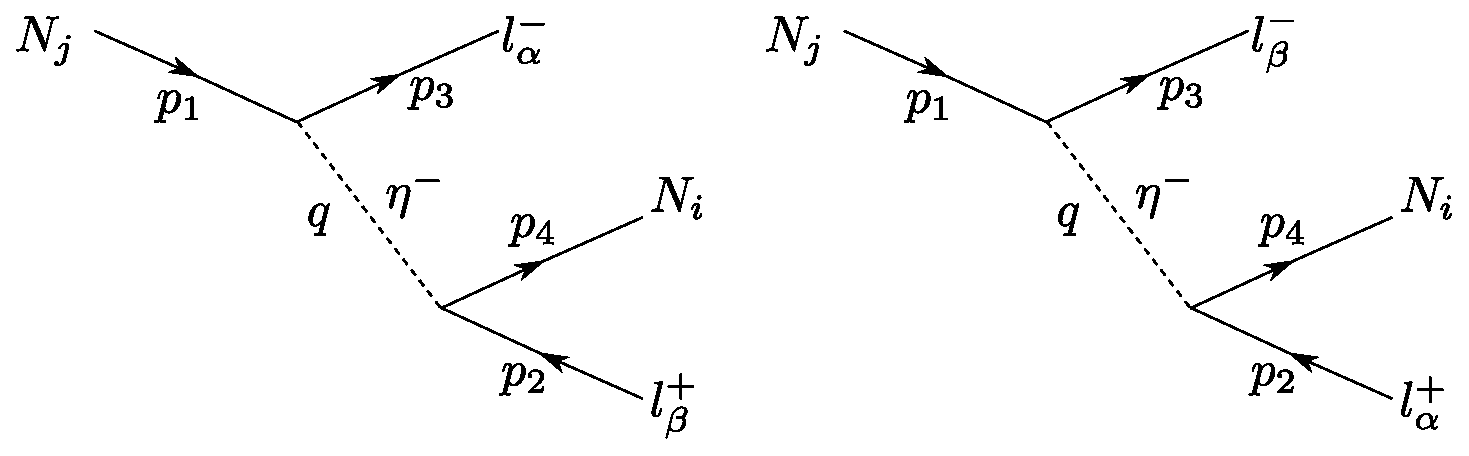
\includegraphics[scale=0.7]{nj_decay} %noinstiki
  \caption{Tree level diagram for $N_j$ decay } %noinstiki
  \label{fig:2} %noinstiki
\end{figure} %noinstiki


we have the amplitude 
\begin{align}
  \mathcal{M}=&-i
  h_{\alpha j}\bar{u}_3(1-\gamma_5)u_1\left(\frac{1}{q^2-M_\eta^2}\right)h_{\beta i}\bar{u}_4(1-\gamma_5)v_2\nonumber\\
  &-i h_{\beta j}\bar{u}_3(1-\gamma_5)u_1\left(\frac{1}{q^2-M_\eta^2}\right)h_{\alpha i}\bar{u}_4(1-\gamma_5)v_2\nonumber\\
  \approx&-\frac{iH_{\alpha\beta ij}}{{M_\eta^2}}\bar{u}_3(1-\gamma_5)u_1\bar{u}_4(1-\gamma_5)v_2
\end{align}
where
\begin{equation}
  H_{\alpha\beta ij}=h_{\alpha j}h_{\beta i}+h_{\alpha i}h_{\beta j}
\end{equation}
\begin{align}
   \mathcal{M}^*=&-\frac{iH_{\alpha\beta ij}}{{M_\eta^2}}
   [\bar{u}_3(1-\gamma_5)u_1]^\dagger[\bar{u}_4(1-\gamma_5)v_2]^\dagger\nonumber\\
   =&-\frac{iH_{\alpha\beta ij}}{{M_\eta^2}}[\bar{u}_1(1+\gamma_5)u_3][\bar{v}_2(1+\gamma_5)u_4]\,.
\end{align}

Multiplying $\mathcal{M}$ and $\mathcal{M}^*$ we have
\begin{align}
\left|\mathcal{M}\right|^2=&\frac{H_{\alpha \beta i j}^2}{M_\eta^4}
[\bar{u}_3^\alpha(1-\gamma_5)_{\alpha\beta}u_1^\beta\bar{u}_1^\gamma(1+\gamma_5)_{\gamma\delta}u_3^\delta]
[\bar{u}_4^\alpha(1-\gamma_5)_{\alpha\beta}v_2^\beta\bar{v}_2^\gamma(1+\gamma_5)_{\gamma\delta}u_4^\delta]\nonumber\\
  =&\frac{H_{\alpha\beta i j}^2}{M_\eta^4}
[u_3^\delta\bar{u}_3^\alpha(1-\gamma_5)_{\alpha\beta}u_1^\beta\bar{u}_1^\gamma(1+\gamma_5)_{\gamma\delta}]
[u_4^\delta\bar{u}_4^\alpha(1-\gamma_5)_{\alpha\beta}v_2^\beta\bar{v}_2^\gamma(1+\gamma_5)_{\gamma\delta}]\nonumber\\
  =&\frac{H_{\alpha\beta i j}^2}{M_\eta^4}
[(u_3\bar{u}_3)_{\delta\alpha}(1-\gamma_5)_{\alpha\beta}(u_1\bar{u}_1)_{\beta\gamma}(1+\gamma_5)_{\gamma\delta}]
[(u_4\bar{u}_4)_{\delta\alpha}(1-\gamma_5)_{\alpha\beta}(v_2\bar{v}_2)_{\beta\gamma}(1+\gamma_5)_{\gamma\delta}]\nonumber\\
=&\frac{H_{\alpha\beta i j}^2}{M_\eta^4}
\operatorname{Tr}[(u_3\bar{u}_3)(1-\gamma_5)(u_1\bar{u}_1)(1+\gamma_5)]
\operatorname{Tr}[(u_4\bar{u}_4)(1-\gamma_5)(v_2\bar{v}_2)(1+\gamma_5)]
\end{align}
Using eq.~\eqref{eq:111}, and neglecting charged fermion masses
\begin{align}
\left|\mathcal{M}\right|^2=&\frac{H_{\alpha\beta i j}^2}{M_\eta^4}
\operatorname{Tr}[\cancel{p}_3(1-\gamma_5)(\cancel{p}_1+M_j)(1+\gamma_5)]
\operatorname{Tr}[(\cancel{p}_4+M_i)(1-\gamma_5)\cancel{p}_2(1+\gamma_5)]\nonumber\\
=&\frac{H_{\alpha\beta i j}^2}{M_\eta^4} L M
\end{align}
\begin{align}
  L=&\operatorname{Tr}[(\cancel{p}_3-\cancel{p}_3\gamma_5)(\cancel{p}_1+\cancel{p}_1\gamma_5+M_j+M_j\gamma_5]
\end{align}
\begin{align}
  L=&\operatorname{Tr}[\cancel{p}_3\cancel{p}_1+\cancel{p}_3\cancel{p}_1\gamma_5+M_j\cancel{p}_3+M_j\cancel{p}_3\gamma_5-\cancel{p}_3\gamma_5\cancel{p}_1-\cancel{p}_3\gamma_5\cancel{p}_1\gamma_5-\cancel{p}_3\gamma_5M_j+M_j\gamma_5]\nonumber\\
  =&2\operatorname{Tr}[\cancel{p}_3\cancel{p}_1]\nonumber\\
  =&2p_3^\alpha p_1^\beta\operatorname{Tr}[\gamma_\alpha\gamma_\beta]\nonumber\\
  =&8p_3^\alpha p_1^\beta g_{\alpha\beta}\nonumber\\
  =&8(p_3\cdot p_1)
\end{align}
Similarly
\begin{align}
  M=8(p_4\cdot p_2)
\end{align}
Therefore
\begin{align}
  \left|\mathcal{M}\right|^2=&\frac{H_{\alpha\beta i j}^2}{M_\eta^4}64(p_3\cdot p_4)(p_1\cdot p_2)\nonumber\\
  \left|\mathcal{M}\right|^2=&\frac{H_{\alpha\beta i j}^2}{4M_\eta^4}4\times64(p_3\cdot p_4)(p_1\cdot p_2)\nonumber\\
\end{align}
In this way, comparing with eq.~\eqref{eq:112}, the results for the moun decay can be directly used after the replacements
\begin{align}
  \frac{g^4}{64 M_W^4}&\to\frac{H_{\alpha\beta i j}^2}{4M_\eta^4}\nonumber\\
  \frac{g^4}{M_W^4}&\to\frac{16H_{\alpha\beta i j}^2}{M_\eta^4}\nonumber\\
  m_\mu&\to M_j\nonumber\\
  x=\frac{m_e}{m_\mu}&\to\frac{M_i}{M_j}\,.
\end{align}
The decay width is according eq.~\eqref{eq:120}
\begin{align}
  \label{eq:121}
  \Gamma(N_j\to l_\alpha^\mp l_\beta^\pm N_i)=&\frac{16H_{\alpha\beta ij}^2}{M_\eta^4}
  \frac{4}{192 (2\pi)^3 M_j }\frac{M_j^6}{16}I\left(x\right)\nonumber\\
=&\frac{(h_{\alpha j}h_{\beta i}+h_{\alpha i}h_{\beta j})^2}{2 M_\eta^4}
  \frac{M_j^5}{192 \pi^3}{}I\left(x\right)
\end{align}
where
\begin{align}
  I(x)=1-8x^2-24x^4\ln(x)+8x^6-x^8\,,\qquad x=\frac{M_i}{M_j}\,.
\end{align}
Similarly the decay through $\eta^0$ is
\begin{align}
  \label{eq:122}
   \Gamma(N_j\to\nu_\alpha\nu_\beta N_i)
=&\frac{(h_{\alpha j}h_{\beta i}+h_{\alpha i}h_{\beta j})^2}{2 M_{\eta^0}^4}
  \frac{M_j^5}{192 \pi^3}{}I\left(x\right)
\end{align}
In this way, for example for $N_2$
\begin{align}
  \sum_{\alpha}\Gamma(N_2\to l_\alpha^- l_\beta^+ N_1)=&\sum_\alpha\frac{h_{\alpha2}^2h_{\beta1}^2+h_{\alpha1}^2h_{\beta2}^2+2h_{\alpha2}h_{\alpha1}h_{\beta2}h_{\beta1}}{2 M_\eta^4}
  \frac{M_2^5}{192 \pi^3}{}I\left(x\right)\nonumber\\
 =&\frac{\mathbf{h}_2^2h^2_{\beta1}+\mathbf{h}_1^2h^2_{\beta2}+2\mathbf{h}_2\cdot\mathbf{h}_1h_{\beta2}h_{\beta1}}{2 M_\eta^4}
  \frac{M_2^5}{192 \pi^3}{}I\left(x\right)
\end{align}
\begin{align}
  \sum_{\alpha\beta}\Gamma(N_2\to l_\alpha^- l_\beta^+ N_1)=&\frac{\mathbf{h}_2^2\mathbf{h}_1^2+\mathbf{h}_1^2\mathbf{h}_2^2
    +2(\mathbf{h}_2\cdot\mathbf{h}_1)^2}{2 M_\eta^4}
  \frac{M_2^5}{192 \pi^3}I\left(x\right)\nonumber\\
=&\frac{\mathbf{h}_1^2\mathbf{h}_2^2
    +(\mathbf{h}_1\cdot\mathbf{h}_2)^2}{M_\eta^4}
  \frac{M_2^5}{192 \pi^3}{}I\left(x\right)
 \end{align}
In general
\begin{align}
  \label{eq:123}
    \sum_{\alpha\beta}\Gamma(N_j\to l_\alpha^- l_\beta^+ N_i)
=&\frac{\mathbf{h}_i^2\mathbf{h}_j^2
    +(\mathbf{h}_i\cdot\mathbf{h}_j)^2}{M_\eta^4}
  \frac{M_j^5}{192 \pi^3}{}I\left(\frac{M_i}{M_j}\right)\nonumber\\
    \sum_{\alpha\beta}\Gamma(N_j\to \nu_\alpha \nu_\beta N_i)
=&\frac{\mathbf{h}_i^2\mathbf{h}_j^2
    +(\mathbf{h}_i\cdot\mathbf{h}_j)^2}{M_{\eta^0}^4}
  \frac{M_j^5}{192 \pi^3}{}I\left(\frac{M_i}{M_j}\right)
\end{align}
For fix $i$ and $j$
\begin{align}
  \label{eq:124}
  \frac{\sum_{\alpha\beta}\operatorname{Br}(N_j\to l_\alpha^- l_\beta^+ N_i)}{\sum_{\alpha\beta}\operatorname{Br}(N_j\to \nu_\alpha \nu_\beta N_i)}=
\frac{M_{\eta^0}^4}{M_{\eta^\pm}^4}
\end{align}
while for 
\begin{align}
  \label{eq:125}
  \frac{\sum_{\alpha\beta}\operatorname{Br}(N_3\to\nu_\alpha\nu_\beta N_2)}{\sum_{\alpha\beta}\operatorname{Br}(N_3\to l_\alpha^-l_\beta^+ N_1)}\approx&
  \frac{\mathbf{h}_2^2\mathbf{h}_3^2
    +(\mathbf{h}_2\cdot\mathbf{h}_3)^2}{\mathbf{h}_1^2\mathbf{h}_3^2
    +(\mathbf{h}_1\cdot\mathbf{h}_3)^2}\frac{M_{\eta^\pm}^4}{M_{\eta^0}^4}I(M_2/M_3)\nonumber\\
  \frac{\sum_{\alpha\beta}\operatorname{Br}(N_3\to l_\alpha^-l_\beta^+ N_2)}{\sum_{\alpha\beta}\operatorname{Br}(N_3\to l_\alpha^-l_\beta^+ N_1)}\approx&
  \frac{\mathbf{h}_2^2\mathbf{h}_3^2
    +(\mathbf{h}_2\cdot\mathbf{h}_3)^2}{\mathbf{h}_1^2\mathbf{h}_3^2
    +(\mathbf{h}_1\cdot\mathbf{h}_3)^2}I(M_2/M_3)
\end{align}

For $N_2$ the total decay width is
\begin{align}
  \Gamma_{\text{tot}}(N_2)=&\left[{\mathbf{h}_1^2\mathbf{h}_2^2
    +(\mathbf{h}_1\cdot\mathbf{h}_2)^2}\right]
  \frac{M_2^5}{192 \pi^3}I\left(\frac{M_1}{M_2}\right)\left[\frac{1}{M_{\eta^\pm}^4}+\frac{1}{M_{\eta^0}^4}\right]
\end{align}
And the individual branchings through $\eta^\pm$ given by eq.~\eqref{eq:121}.

For $N_3$ we have several possibilities for signals with charged leptons. The cleanest one is when $N_3$ decay only through $\eta^\pm$ through an intermediate $N_2$. 

The branching of $N_3$ to two charged leptons plus missing energy is either
\begin{align}
  \label{eq:126}
  \operatorname{Br}(N_3\to l_\alpha^\pm l_\beta^\mp N_1)
\end{align}
where the $N_3$ is reconstructed, or
\begin{align}
  \label{eq:127}
  \operatorname{Br}(N_3\underbrace{\to}_{\eta^0}l_\alpha^\pm l_\beta^\mp N_1)=\operatorname{Br}(N_3\to\nu_\alpha  \nu_\beta N_2)\times\operatorname{Br}(N_2\to l_\alpha^\pm  l_\beta^\mp N_1)
\end{align}
that seem to be very difficult to reconstruct. This also seem to be an irreducible background for
\begin{align}
  \operatorname{Br}(N_2\to l_\alpha^\pm  l_\beta^\mp N_1)
\end{align}
To get rid of processes like the one in eq.~\eqref{eq:127}  must be $\operatorname{Br}(N_3\to\nu_\alpha  \nu_\beta N_2)$ is suppressed. This happens if
\begin{itemize} %noinstiki
\item %noinstiki
 $I(M_2/M3)\ll1$. In this case the mutilepton signal for $N_3$ is also suppressed. Clearly this happens for $M_2\approx M_3$ as $I(x)$ is a sharpest function which controls the kinematical suppression. We show below for an specific point that even for $M_3-M_2\approx20\,$GeV, we can have the Branching in eq.~\eqref{eq:126} sufficiently large.

\item %noinstiki 
$M_{\eta^\pm}\ll M_{\eta^0}$

\end{itemize} %noinstiki


In appendix \ref{sec:sample-point}, it is shown a full set of yukawas consistent with neutrino physics. For this solution 
\begin{align}
  \frac{\operatorname{Br}(\eta^+\to N_3)}{\operatorname{Br}(\eta^+\to N_1)}\approx&0.61&
  \frac{\operatorname{Br}(\eta^+\to N_2)}{\operatorname{Br}(\eta^+\to N_1)}\approx&0.37&\nonumber\\
  {\operatorname{Br}(\eta^+\to N_1)}\approx&0.51&  {\operatorname{Br}(\eta^+\to N_2)}\approx&0.19 & {\operatorname{Br}(\eta^+\to N_3)}\approx&0.30
\end{align}
Below we estimate the branchings to $N_3\to l_\alpha^-l_\beta^+ N_1$ or $N_3\to\nu_\alpha\nu_\beta N_2\to\nu_\alpha\nu_\beta l_\alpha^-l_\beta^+ N_1$. For this we need the Branchings
for $N_2\to l_\alpha^-l_\beta^+ N_1$ compared with Branching to $N_2\to\nu_\alpha\nu_\beta N_1$. In general this is
From this, the visible decays are using eq.~(\ref{eq:124}) 
\begin{align}
   \frac{\sum_{\alpha\beta}\operatorname{Br}(N_2\to l_\alpha^- l_\beta^+ N_1)}{\sum_{\alpha\beta}\operatorname{Br}(N_2\to \nu_\alpha \nu_\beta N_1)}\approx&0.758
   \Rightarrow&\sum_{\alpha\beta} \operatorname{Br}(N_2\to l_\alpha^- l_\beta^+ N_1)=0.431
\end{align}
On the other hand the chanels for $N_3$ are $N_3\to l_\alpha^-l_\beta^+ N_1$, $N_3\to\nu_\alpha\nu_\beta N_1$, $N_3\to l_\alpha^-l_\beta^+ N_2$, and $N_3\to\nu_\alpha\nu_\beta N_2$.
From eqs.~\eqref{eq:124} \eqref{eq:125}
\begin{align}
  \frac{\sum_{\alpha\beta}\operatorname{Br}(N_3\to\nu_\alpha\nu_\beta N_2)}{\sum_{\alpha\beta}\operatorname{Br}(N_3\to l_\alpha^-l_\beta^+ N_1)}
  &\approx0.0812& 
  \frac{\sum_{\alpha\beta}\operatorname{Br}(N_3\to l_\alpha^-l_\beta^+ N_2)}{\sum_{\alpha\beta}\operatorname{Br}(N_3\to l_\alpha^-l_\beta^+ N_1)}
  &\approx0.0615\nonumber\\
\frac{\sum_{\alpha\beta}\operatorname{Br}(N_3\to\nu_\alpha\nu_\beta N_1)}{\sum_{\alpha\beta}\operatorname{Br}(N_3\to l_\alpha^-l_\beta^+ N_1)}
  &\approx1.320
\end{align}
\begin{align}
  \sum_{\alpha\beta}\operatorname{Br}(N_3\to l_\alpha^-l_\beta^+ N_1)&\approx\frac{1}{1+0.0812+0.0615+1.320}=0.406\nonumber\\ 
  \sum_{\alpha\beta}\operatorname{Br}(N_3\to\nu_\alpha\nu_\beta N_1)&\approx0.536\nonumber\\
  \sum_{\alpha\beta}\operatorname{Br}(N_3\to\nu_\alpha\nu_\beta N_2)&\approx0.030\nonumber\\
  \sum_{\alpha\beta}\operatorname{Br}(N_3\to l_\alpha^-l_\beta^+ N_2)&\approx0.025
\end{align}
The expected background for $N_{2,3}\to l_\alpha^-l_\beta^+ N_1$ is 

\begin{equation}
  \sum_{\alpha\beta}\operatorname{Br}(N_3\to\nu_\alpha\nu_\beta N_2)\times\sum_{\alpha\beta}\operatorname{Br}(N_2\to l_\alpha^-l_\beta^+ N_1)\approx0.030\times0.431=0.013
\end{equation}


We have that
\begin{align*}
 \Gamma_{tot}(N_2)=&\left[{\bf h}^2_1{\bf h}^2_2+({\bf h}_1\cdot {\bf h}_2)^2\right]\frac{M_2^5}{192\pi^3}I\left(\frac{M_1}{M_2} \right)\left[ \frac{1}{M^4_{\eta^\pm}}+\frac{1}{M^4_{\eta^0}}\right]\\
\Gamma_{vis}(N_2\to N_1)\equiv& \sum_{\alpha\beta}\Gamma(N_2\to l_\alpha^- l_\beta^+ N_1)\\
   =&\frac{{\bf h}^2_1{\bf h}^2_2+({\bf h}_1\cdot {\bf h}_2)^2}{M^4_{\eta^\pm}}\frac{M_2^5}{192\pi^3}I\left(\frac{M_1}{M_2} \right)\\
\Gamma_{vis}(N_3\to N_1)\equiv& \sum_{\alpha\beta}\Gamma(N_3\to l_\alpha^- l_\beta^+ N_1)\\
   =&\frac{{\bf h}^2_1{\bf h}^2_3+({\bf h}_1\cdot {\bf h}_3)^2}{M^4_{\eta^\pm}}\frac{M_3^5}{192\pi^3}I\left(\frac{M_1}{M_3} \right)\\
\Gamma_{invis}(N_3\to N_2)\equiv& \sum_{\alpha\beta}\Gamma(N_3\to \nu_\alpha \nu_\beta N_2)\\
   =&\frac{{\bf h}^2_2{\bf h}^2_3+({\bf h}_2\cdot {\bf h}_3)^2}{M^4_{\eta^0}}\frac{M_3^5}{192\pi^3}I\left(\frac{M_2}{M_3} \right).
\end{align*}
From above equations we can obtain the following observable:
\begin{align*}
 &\frac{\mbox{Br}_{invis}(N_3\to N_2)\times \mbox{Br}_{vis}(N_2\to N_1)}{\mbox{Br}_{vis}(N_3\to N_1)}\\
&=\frac{\frac{{\bf h}^2_2{\bf h}^2_3+({\bf h}_2\cdot {\bf h}_3)^2}{M^4_{\eta^0}}\frac{M_3^5}{192\pi^3}I\left(\frac{M_2}{M_3} \right)\times \frac{{\bf h}^2_1{\bf h}^2_2+({\bf h}_1\cdot {\bf h}_2)^2}{M^4_{\eta^\pm}}\frac{M_2^5}{192\pi^3}I\left(\frac{M_1}{M_2} \right)}{\frac{{\bf h}^2_1{\bf h}^2_3+({\bf h}_1\cdot {\bf h}_3)^2}{M^4_{\eta^\pm}}\frac{M_3^5}{192\pi^3}I\left(\frac{M_1}{M_3} \right)\Gamma_{tot}(N_2)}\\
&=\frac{{\bf h}^2_2{\bf h}^2_3+({\bf h}_2\cdot {\bf h}_3)^2}{{\bf h}^2_1{\bf h}^2_3+({\bf h}_1\cdot {\bf h}_3)^2}I\left(\frac{M_2}{M_3} \right)\frac{1}{M^4_{\eta^0}\left[\frac{1}{M^4_{\eta^0}}+\frac{1}{M^4_{\eta^\pm}} \right] }\\
&=\frac{{\bf h}^2_2{\bf h}^2_3+({\bf h}_2\cdot {\bf h}_3)^2}{{\bf h}^2_1{\bf h}^2_3+({\bf h}_1\cdot {\bf h}_3)^2}I\left(\frac{M_2}{M_3} \right)\frac{1}{\left[1+\frac{M^4_{\eta^0}}{M^4_{\eta^\pm}} \right]}
\end{align*}
 


% \begin{align}
%   \operatorname{Br}(N_3\to l^\pm l^\mp N_1)=&\sum_{\alpha\beta}\operatorname{Br}(N_3\to l_\alpha^\pm  l_\beta^\mp N_1)+
% \sum_{\alpha\beta}\operatorname{Br}(N_3\to\nu_\alpha  \nu_\beta N_2)\times\sum_{\alpha\beta}\operatorname{Br}(N_2\to l_\alpha^\pm  l_\beta^\mp N_1)\nonumber\\
% \end{align}
% \begin{align}
%   =&\frac{1}{\Gamma_{\text{tor}}(N_3)}\frac{\left[\mathbf{h}_1^2\mathbf{h}_3^2
%     +(\mathbf{h}_1\cdot\mathbf{h}_3)^2\right]}{192\pi^3}
% \end{align}

%\appendix{}
\begin{subappendices} %noinstiki
  

\section{Sample point}
\label{sec:sample-point}

\begin{verbatim} 
       write(32,*) (h(i,1),i=1,3),(h(i,2),i=1,3),(h(i,3),i=1,3)
\end{verbatim} %noinstiki

\begin{verbatim} 
 -0.00188878597  0.000780236776  0.000248251388 
 -0.000352494763 -0.000180683976 -0.00122443053  
  0.000392272581  0.00120920029 -0.0012245638
\end{verbatim} %noinstiki

So that
\begin{align}
  \mathbf{h}_1^2&\approx4.238\times10^{-6}&\mathbf{h}_2^2&\approx1.656\times10^{-6}\nonumber\\
  \mathbf{h}_3^2&\approx3.116\times10^{-6} & \mathbf{h}_1\cdot\mathbf{h}_2&\approx2.208\times10^{-7}\nonumber\\
\mathbf{h}_1\cdot\mathbf{h}_3&\approx1.015\times10^{-7}& \mathbf{h}_2\cdot\mathbf{h}_3\approx&1.143\times10^{-6}
\end{align}
\begin{align}
  \mathbf{h}_1^2\mathbf{h}_2^2+(\mathbf{h}_1\cdot\mathbf{h}_2)^2\approx&7.067\times10^{-12}
  &\mathbf{h}_1^2\mathbf{h}_3^2+(\mathbf{h}_1\cdot\mathbf{h}_3)^2\approx&1.321\times10^{-11}\nonumber\\
  \mathbf{h}_2^2\mathbf{h}_3^2+(\mathbf{h}_2\cdot\mathbf{h}_3)^2\approx&6.465\times10^{-12}
\end{align}
The spectrum consistent with neutrino data is
\begin{align}
  M_1\approx&6.16918656\,\text{KeV} &M_2\approx&22.8695451\,\text{GeV}  &M_3\approx&43.126911\,\text{GeV}\nonumber\\
  M_{\eta^0}\approx&139.1382\,\text{GeV}& M_{\eta^\pm}\approx&149.1382\,\text{GeV}
\end{align}
\begin{align}
  I(M_1/M_3)\approx&1 & I(M_2/M_3)\approx&0.126
\end{align}

\section{Preliminary discussion}
\label{sec:prel-disc}

One interesting possibility in view of the large invisible direct decay, like $N_3\to\nu_\alpha\nu_\beta N_1$, is to get the observables from the missing plus one energetic lepton (coming from $\eta^+$)  signal. May be decays like
\begin{align}
  \eta^+&\to l_\alpha^+ N_3 \to l_\alpha^+ \;\cancel{E}_T\nonumber\\
  \eta^+&\to l_\alpha^+ N_2 \to l_\alpha^+ \;\cancel{E}_T\nonumber\\
\end{align}

Once $\eta^0_{R,I}$, or $\eta^\pm$ are produced the full list of signals is: 
For $\eta^\pm$ production. The decay to $N_j$  is
\begin{align}
\Gamma(\eta^+\to l_\alpha^+ N_j)=\frac{3h_{\alpha j}^2}{16\pi M_\eta}\lambda^{1/2}\left(M_\eta^2,M_j^2,m_\alpha^2\right)\left(1-\frac{M_j^2+m_\alpha^2}{M_\eta^2}\right)
\end{align}
\begin{align}
  \sum_\alpha\Gamma(\eta^+\to l_\alpha^+ N_j)=\frac{3\mathbf{h}_j^2}{16\pi M_\eta}\lambda^{1/2}\left(M_\eta^2,M_j^2,m_\alpha^2\right)\left(1-\frac{M_j^2+m_\alpha^2}{M_\eta^2}\right)
\end{align}
with
\begin{align}
  \lambda^{1/2}\left(M_\eta^2,M_j^2,m_\alpha^2\right)=\left[\left(M_\eta^2+M_j^2-m_\alpha^2\right)^2-4M_\eta^2M_j^2\right]^{1/2}
\end{align}
Neglecting $m_\alpha$ with respect to $N_{2,3}$, we have for $j=2,3$
\begin{align}
  \lambda^{1/2}\left(M_\eta^2,M_j^2,m_\alpha^2\right)\approx&M_\eta^2\left[\left(1+\frac{M_j^2}{M_\eta^2}\right)^2-\frac{4M_j^2}{M_\eta^2}\right]^{1/2}\nonumber\\
  \approx&M_\eta^2\left[1+2\frac{M_j^2}{M_\eta^2}-\frac{4M_j^2}{M_\eta^2}\right]^{1/2}\nonumber\\
  \approx&M_\eta^2\left[1-2\frac{M_j^2}{M_\eta^2}\right]^{1/2}\nonumber\\
  \approx&M_\eta^2\left[1-\frac{M_j^2}{M_\eta^2}\right]
\end{align}
Therefore
\begin{align}
   \sum_\alpha\Gamma(\eta^+\to l_\alpha^+ N_j)\approx&\frac{3\mathbf{h}_j^2M_\eta}{16\pi}\times
   \begin{cases}
     \displaystyle{\left(1-\frac{M_j^2}{M_\eta^2}\right)^2} & j=2,3\\
     1 & j=1
   \end{cases}\nonumber\\
   \approx&\frac{3\mathbf{h}_j^2M_\eta}{16\pi}\times
   \begin{cases}
     \displaystyle{\left(1-2\frac{M_j^2}{M_\eta^2}\right)} & j=2,3\\
     1 & j=1
   \end{cases}\nonumber\\
\end{align}
In this way
\begin{align}
  \Gamma_{\text{tor}}(\eta^+)=&\sum_{\alpha j}\Gamma(\eta^+\to l_\alpha^+ N_j)\nonumber\\
  \approx&\frac{3M_\eta}{16\pi}\left[\mathbf{h}_1^2
    +\mathbf{h}_2^2\left(1-2\frac{M_2^2}{M_\eta^2}\right)
    +\mathbf{h}_3^2\left(1-2\frac{M_3^2}{M_\eta^2}\right)\right]
\end{align}

\begin{align}
\frac{\operatorname{Br}(\eta^+\to N_j)}{\operatorname{Br}(\eta^+\to N_i)}=&  \frac{\sum_\alpha\Gamma(\eta^+\to l_\alpha^+ N_j)}{\sum_\alpha\Gamma(\eta^+\to l_\alpha^+ N_i)}\nonumber\\
\approx&\frac{\mathbf{h}_j^2}{\mathbf{h}_i^2}\frac{1-2M_j^2/M_\eta^2}{1-2M_i^2/M_\eta^2}\nonumber\\
 \approx&\frac{\mathbf{h}_j^2}{\mathbf{h}_i^2}(1-2M_j^2/M_\eta^2)(1-2M_i^2/M_\eta^2)^{-1}\nonumber\\
  \approx&\frac{\mathbf{h}_j^2}{\mathbf{h}_i^2}(1-2M_j^2/M_\eta^2)(1+2M_i^2/M_\eta^2)\nonumber\\
  \approx&\frac{\mathbf{h}_j^2}{\mathbf{h}_i^2}\left[1-2\left(\frac{M_j^2-M_i^2}{M_\eta^2}\right)\right]
\end{align}
For three branchings we should have

\begin{align}
  a+b+c&=1\nonumber\\
1+\frac{b}{a}+\frac{c}{a}&=\frac{1}{a}\nonumber\\
{a}&=\frac{1}{1+{b}/{a}+{c}/{a}}
\end{align}
In this way
\begin{align}
  {\operatorname{Br}(\eta^+\to N_1)}=\frac{1}{1+\frac{\operatorname{Br}(\eta^+\to N_3)}{\operatorname{Br}(\eta^+\to N_1)}+\frac{\operatorname{Br}(\eta^+\to N_3)}{\operatorname{Br}(\eta^+\to N_1)}}
\end{align}

From eq.%~\eqref{eq:75}
\begin{align}
  \frac{\operatorname{Br}\left(N_3\to N_1\right)}
{\operatorname{Br}(N_3\underbrace{\to}_{\eta^\pm}N_2)}=&
\end{align}

\end{subappendices} %noinstiki


%\left(\right)
%\left|\mathcal{M}\right|
%%% Local Variables: 
%%% mode: latex
%%% TeX-master: "beyond"
%%% End:
\include{renormalization}
\begin{thebibliography}{99}
\bibitem{lsm} Diego Restrepo, Hac\'\i a la teor\'\i a cu\'antica de campos, curso web, \url{http://gfif.udea.edu.co}

\bibitem{Maggiore:2005qv}
  M.~Maggiore,
  ``A Modern introduction to quantum field theory,''
%\href{http://www.slac.stanford.edu/spires/find/hep/www?irn=6374123}{SPIRES entry}
{\it  Oxford University Press, 2005. (Oxford Series in Physics, 12. ISBN 0 19 852073 5)}

\bibitem{Mandl:1985bg}
  F.~Mandl and G.~Shaw,
  %``Quantum Field Theory,''
%\href{http://www.slac.stanford.edu/spires/find/hep/www?irn=1457594}{SPIRES entry}
{\it  Chichester, Uk: Wiley ( 1984) 354 P. ( A Wiley-interscience Publication)}

\bibitem{Lahiri:2005sm}
  A.~Lahiri and P.~B.~Pal,
  ``A first book of quantum field theory,''
%\href{http://www.slac.stanford.edu/spires/find/hep/www?irn=6927483}{SPIRES entry}
{\it  Harrow, UK: Alpha Sci. Int. (2005) 380 p}

\bibitem{physics/0703214} Pal, P. ``Representation-independent manipulations with Dirac matrices and spinors'',
	arXiv:physics/0703214v2 [physics.ed-ph]

\bibitem{PD} Wikipedia article: \url{http://en.wikipedia.org/wiki/Particle_decay}

\bibitem{Klasen:2002xi}
  M.~Klasen,
  %``Calculating two- and three-body decays with FeynArts and FormCalc,''
  Int.\ J.\ Mod.\ Phys.\  C {\bf 14} (2003) 1273
  [arXiv:hep-ph/0210426].
  %%CITATION = IMPAE,C14,1273;%%

\bibitem{PeterRenton} \emph{Electroweak Interactions}, Peter Renton


\bibitem{Peskin}
Michael E. Peskin and Daniel V. Schroeder. \emph{An introduction to
Quantum Field Theory}, Addison-Wesley Publishing Company(1995), p.
101

\bibitem{Peskin1}
ibdg 1, p. 105

\bibitem{Halzen}
Francis Halzen and Alan D. Martin. \emph{Quarks} \& \emph{Leptons:
An introductory Course in Modern Particle Physics}, John Wiley \&
Sons(1984), p. 89

\bibitem{Quigg}
Chris Quigg. \emph{Gauge theory of the Strong, Weak and
Electromagnetic Interactions}, Westview Press(1997), p. 110


\bibitem{Quigg1}
ibdg 4, p. 130.

\bibitem{Mandl1}
ibdg 5, p. 325.


\bibitem{Sierra:2008wj}
  D.~Aristizabal Sierra, J.~Kubo, D.~Restrepo, D.~Suematsu and O.~Zapata,
  ``Radiative seesaw: Warm dark matter, collider and lepton flavour violating
  signals,''
  Phys.\ Rev.\  D {\bf 79} (2009) 013011
  [arXiv:0808.3340 [hep-ph]].
  %%CITATION = PHRVA,D79,013011;%%

\bibitem{Gross:1993} 
Relativistic Quantum Mechanics and Field Theory, Franz Gross, John Wiley \& Sons, INC. 1993

\bibitem{McMahon:2009zz}
  D.~McMahon,
  ``Quantum field theory demystified: A self-teaching guide,''
  \href{http://www.slac.stanford.edu/spires/find/hep/www?irn=8432112}{SPIRES entry}
{\it  New York, USA: McGraw-Hill (2009) 299 p}

\bibitem{Feynman:1986er}
  R.~P.~Feynman,
  ``QED. The Strange Theory Of Light And Matter,''
%\href{http://www.slac.stanford.edu/spires/find/hep/www?irn=1631209}{SPIRES entry}
{\it  Princeton, Usa: Univ. Pr. ( 1985) 158 P. ( Alix G. Mautner Memorial Lectures)}


\bibitem{Semenov:2008jy}
  A.~Semenov,
  ``LanHEP - a package for the automatic generation of Feynman rules in field
  theory. Version 3.0,''
  Comput.\ Phys.\ Commun.\  {\bf 180} (2009) 431
  [arXiv:0805.0555 [hep-ph]], \url{http://feynrules.phys.ucl.ac.be/}.
  %%CITATION = CPHCB,180,431;%%

\bibitem{Christensen:2008py}
  N.~D.~Christensen and C.~Duhr,
  ``FeynRules - Feynman rules made easy,''
  Comput.\ Phys.\ Commun.\  {\bf 180}, 1614 (2009)
  [arXiv:0806.4194 [hep-ph]],
   \url{http://feynrules.phys.ucl.ac.be/}.
  %%CITATION = CPHCB,180,1614;%%

\bibitem{massivephoton}
  Christianto V., Smarandache F., and Lichtenberg F., 
  ``\href{http://www.ptep-online.com/index_files/2009/PP-16-08.PDF}{A Note of Extended Proca Equations and Superconductivity,}''
  Progress in Physics, \textbf{1} (2009) 40
  [viXra:1003.0054]

\end{thebibliography}
%%% Local Variables: 
%%% mode: latex
%%% TeX-master: "beyond"
%%% End:

\end{document}


%%% Local Variables: 
%%% mode: latex
%%% TeX-master: "beyond"
%%% End: 
